% \documentclass[12pt,b5paper]{report}
\documentclass[12pt,a4paper]{report}
\usepackage[utf8]{inputenc}
\usepackage[T1]{fontenc}
\usepackage{amsmath}
\usepackage{amsfonts}
\usepackage{amssymb}
\usepackage[left=2cm,right=2cm,top=2cm,bottom=2cm]{geometry}
\usepackage{graphicx}

% \usepackage{nonfloat}

\usepackage{multicol}
\usepackage{xcolor}
\definecolor{electricgreen}{rgb}{0.0, 1.0, 0.0}

\usepackage{xfrac}
\usepackage{lscape}

% \usepackage[toc,page]{appendix}
\usepackage[titletoc]{appendix}

\usepackage{url}
\usepackage{cite}
\usepackage{rotating}

\usepackage{bibentry}
\nobibliography*

% \usepackage{caption}
\usepackage{subcaption}
\usepackage{slashed}
\usepackage{lineno}
\usepackage{siunitx}
\usepackage{xspace}
\usepackage{tikz}
\usepackage{fancyhdr}

\usepackage{arydshln}

% Continuous figure/table numbers
\usepackage{chngcntr}
\counterwithout{figure}{chapter}
\counterwithout{table}{chapter}

% Use shaped lines
\makeatletter
\pgfkeys{
	/tikz/sharp arrow angle/.code={%
    	\pgfsetarrowoptions{sharp left}{#1}
    	\pgfsetarrowoptions{sharp right}{#1}
  	},
	/tikz/sharp left arrow angle/.code={%
	    \pgfsetarrowoptions{sharp left}{#1}
	},
	/tikz/sharp right arrow angle/.code={%
	    \pgfsetarrowoptions{sharp right}{#1}
	}
}
\tikzset{
	sharp arrow angle=30
}
\pgfarrowsdeclare{sharp left}{sharp left}{%
	  \pgfmathsetlength{\pgf@xa}{.5*\pgflinewidth * tan(\pgfgetarrowoptions{sharp left})}
	  \pgfarrowsleftextend{\pgf@xa}
	  \pgfarrowsrightextend{\pgf@xa}
}{%
  \pgfmathsetlength{\pgf@xa}{\pgflinewidth * tan(\pgfgetarrowoptions{sharp left})}
  \pgfpathmoveto{\pgfqpoint{-.1\pgflinewidth}{-.5\pgflinewidth}}
  \pgfpathlineto{\pgfqpoint{0pt}{-.5\pgflinewidth}}
  \pgfpathlineto{\pgfqpoint{\pgf@xa}{.5\pgflinewidth}}
  \pgfpathlineto{\pgfqpoint{-.1\pgflinewidth}{.5\pgflinewidth}}
  \pgfusepathqfill
}
\pgfarrowsdeclare{sharp right}{sharp right}{%
  \pgfmathsetlength{\pgf@xa}{.5*\pgflinewidth * tan(\pgfgetarrowoptions{sharp right})}
  \pgfarrowsleftextend{\pgf@xa}
  \pgfarrowsrightextend{\pgf@xa}
}{%
  \pgfmathsetlength{\pgf@xa}{\pgflinewidth * tan(\pgfgetarrowoptions{sharp right})}
  \pgfpathmoveto{\pgfqpoint{-.1\pgflinewidth}{.5\pgflinewidth}}
  \pgfpathlineto{\pgfqpoint{0pt}{.5\pgflinewidth}}
  \pgfpathlineto{\pgfqpoint{\pgf@xa}{-.5\pgflinewidth}}
  \pgfpathlineto{\pgfqpoint{-.1\pgflinewidth}{-.5\pgflinewidth}}
  \pgfusepathqfill
}
\makeatother

% Use Feyman
\usepackage{tikz-feynman}
\tikzfeynmanset{
	compat=1.1.0,
	warn luatex=false,
}

% Resize tikz picture
\usepackage{environ}
\newsavebox\mybox
\newenvironment{resizedtikzpicture}[1]{%
  \def\mywidth{#1}%
  \begin{lrbox}{\mybox}%
  \begin{tikzpicture}
}{%
  \end{tikzpicture}%
  \end{lrbox}%
  \resizebox{\mywidth}{!}{\usebox\mybox}%
}

% \renewcommand{\chaptername}{\textsc{Chapter}}
\usepackage[Bjornstrup, Sonny]{fncychap}
\makeatletter
  \ChNameVar{\Large\rm} % sets the style for name
  \ChNumVar{\Huge} % sets the style for digit
  \ChTitleVar{\Huge\rm\bfseries} % sets the style for title
  \ChRuleWidth{4pt} % Set RW=4pt
  \ChNameUpperCase % Make name uppercase
  \renewcommand{\DOCH}{%
    \CNV\FmN{\@chapapp}\space \CNoV\thechapter\par\nobreak
    \vskip 30\p@}
  \renewcommand{\DOTI}[1]{%
    \mghrulefill{1pt}\par\nobreak
    \vskip 11\p@
    \CTV\FmTi{#1}\par\nobreak
    \mghrulefill{1pt}\par\nobreak
    \vskip 50\p@}
  \renewcommand{\DOTIS}[1]{%
    \mghrulefill{1pt}\par\nobreak
    \vskip 11\p@
    \CTV\FmTi{#1}\par\nobreak
    \mghrulefill{1pt}\par\nobreak
    \vskip 50\p@}
\makeatother

\usepackage{hyperref}
\usepackage{cleveref}

\usepackage[toc,nonumberlist,acronym]{glossaries}

\sloppy
% \linenumbers
% TAKEN FROM CMS STYLE GUIDES
\renewcommand{\listfigurename}{Figures and Plots}
\renewcommand{\listtablename}{Tables}

% List of Acronyms
\newcommand{\abbrlabel}[1]{\makebox[3cm][l]{\textbf{#1}\ }}
\newenvironment{abbreviations}{\begin{list}{}{\renewcommand{\makelabel}{\abbrlabel}}}{\end{list}}

% General
\newcommand{\etal}{\mbox{et al.}\xspace} %et al. - no preceding comma
\newcommand{\ie}{\mbox{i.e.}\xspace}     %i.e.
\newcommand{\eg}{\mbox{e.g.}\xspace}     %e.g.
\newcommand{\etc}{\mbox{etc...}\xspace}     %etc.
\newcommand{\vs}{\mbox{\sl vs.}\xspace}      %vs.
\newcommand{\mdash}{\ensuremath{\mathrm{-}}} % for use within formulas
\newcommand{\abs}[1]{\ensuremath{\lvert #1 \rvert}}

% Some software programs and generators
\newcommand{\cmssw}{\textsc{cmssw}\xspace}
\newcommand{\fastjet}{\textsc{FastJet}\xspace}
\newcommand{\geant}{\textsc{Geant4}\xspace}
\newcommand{\herwig}{\textsc{Herwig\raisebox{.1ex}{++}}\xspace}
\newcommand{\powheg}{\textsc{Powheg}\xspace}
\newcommand{\pythia}{\textsc{Pythia}\xspace}
\newcommand{\mgamc}{\textsc{mg5\_}a\textsc{MC@NLO}\xspace}
% \newcommand{\powhegpythia}{\textsc{Powheg\raisebox{.2ex}{+}Pythia}\xspace}
% \newcommand{\powhegherwig}{\textsc{Powheg\raisebox{.2ex}{+}Herwig\raisebox{.1ex}{++}}\xspace}
\newcommand{\mgamcLO}{\textsc{mg5}\_a\textsc{MC@NLO\raisebox{.2ex}{-}LO}\xspace}
\newcommand{\mgamcNLO}{\textsc{mg5}\_a\textsc{MC@NLO\raisebox{.2ex}{-}NLO}\xspace}


% TMP
\newcommand{\POWHEG}{{\textsc{powheg}}\xspace}
\newcommand{\PYTHIA}{{\textsc{pythia}}\xspace}
\newcommand{\HERWIGpp}{{\textsc{herwig++}}\xspace}
\newcommand{\powhegpythia}{\POWHEG{}+\PYTHIA{}\xspace}
\newcommand{\powhegherwig}{\POWHEG{}+\HERWIGpp{}\xspace}
\newcommand{\mgamcMLMpythia}{\textsc{mg5}\_a\textsc{mc@nlo}-\textsc{lo}+\PYTHIA{}\xspace}
\newcommand{\mgamcFxFxpythia}{\textsc{mg5}\_a\textsc{mc@nlo}-\textsc{nlo}+\PYTHIA{}\xspace}
\newcommand{\chis}{\ensuremath{\chi^2}\xspace}


% Measurements and units...
\newcommand{\de}{\ensuremath{^\circ}}
\newcommand{\ten}[1]{\ensuremath{\times \text{10}^\text{#1}}}
\newcommand{\unit}[1]{\ensuremath{\text{~#1}}\xspace}
\newcommand{\pow}[2]{\ensuremath{\mathrm{~#1}^{#2}}\xspace}

\newcommand{\fminv}{\ensuremath{\pow{fm}{-1}}\xspace}
\newcommand{\um}{\ensuremath{\pow{\mu m}{}}\xspace}
\newcommand{\umsq}{\ensuremath{\pow{\mu m}{2}}\xspace}
\newcommand{\mm}{\ensuremath{\pow{mm}{}}\xspace}
\newcommand{\mmsq}{\ensuremath{\pow{mm}{2}}\xspace}
\newcommand{\mmsqinv}{\ensuremath{\pow{mm}{-2}}\xspace}
\newcommand{\cm}{\ensuremath{\pow{cm}{}}\xspace}
\newcommand{\cmsq}{\ensuremath{\pow{cm}{2}}\xspace}
\newcommand{\m}{\ensuremath{\pow{m}{}}\xspace}
\newcommand{\msq}{\ensuremath{\pow{m}{2}}\xspace}
\newcommand{\km}{\ensuremath{\pow{km}{}}\xspace}

\newcommand{\ps}{\ensuremath{\pow{ps}{}}\xspace}
\newcommand{\ns}{\ensuremath{\pow{ns}{}}\xspace}
\newcommand{\us}{\ensuremath{\pow{\mu s}{}}\xspace}
\newcommand{\s}{\ensuremath{\pow{s}{}}\xspace}

\newcommand{\keV}{\ensuremath{\pow{ke\hspace{-.08em}V}{}}\xspace}
\newcommand{\MeV}{\ensuremath{\pow{Me\hspace{-.08em}V}{}}\xspace}
\newcommand{\GeV}{\ensuremath{\pow{Ge\hspace{-.08em}V}{}}\xspace}
\newcommand{\GeVsq}{\ensuremath{\pow{Ge\hspace{-.08em}V}{2}}\xspace}
\newcommand{\TeV}{\ensuremath{\pow{Te\hspace{-.08em}V}{}}\xspace}

\newcommand{\keVc}{\ensuremath{\pow{ke\hspace{-.08em}V}{}\pow{c}{-1}}\xspace}
\newcommand{\MeVc}{\ensuremath{\pow{Me\hspace{-.08em}V}{}\pow{c}{-1}}\xspace}
\newcommand{\GeVc}{\ensuremath{\pow{Ge\hspace{-.08em}V}{}\pow{c}{-1}}\xspace}
\newcommand{\TeVc}{\ensuremath{\pow{Te\hspace{-.08em}V}{}\pow{c}{-1}}\xspace}
\newcommand{\keVcc}{\ensuremath{\pow{ke\hspace{-.08em}V}{}\pow{c}{-2}}\xspace}
\newcommand{\MeVcc}{\ensuremath{\pow{Me\hspace{-.08em}V}{}\pow{c}{-2}}\xspace}
\newcommand{\GeVcc}{\ensuremath{\pow{Ge\hspace{-.08em}V}{}\pow{c}{-2}}\xspace}
\newcommand{\TeVcc}{\ensuremath{\pow{Te\hspace{-.08em}V}{}\pow{c}{-2}}\xspace}

\newcommand{\fb}{\ensuremath{\pow{fb}{}}\xspace}
\newcommand{\fbinv}{\ensuremath{\pow{fb}{-1}}\xspace}
\newcommand{\pb}{\ensuremath{\pow{pb}{}}\xspace}
\newcommand{\pbinv}{\ensuremath{\pow{pb}{-1}}\xspace}
\newcommand{\nb}{\ensuremath{\pow{nb}{}}\xspace}
\newcommand{\nbinv}{\ensuremath{\pow{nb}{-1}}\xspace}
\newcommand{\ub}{\ensuremath{\pow{\mu b}{}}\xspace}
\newcommand{\ubinv}{\ensuremath{\pow{\mu b}{-1}}\xspace}
\newcommand{\mb}{\ensuremath{\pow{mb}{}}\xspace}
\newcommand{\mbinv}{\ensuremath{\pow{mb}{-1}}\xspace}

\newcommand{\Kelvin}{\ensuremath{\pow{K}{}}\xspace}
\newcommand{\Tesla}{\ensuremath{\pow{T}{}}\xspace}
\newcommand{\MHz}{\ensuremath{\pow{MHz}{}}\xspace}

\newcommand{\com}{\ensuremath{\sqrt{s}=13\TeV}\xspace}
\newcommand{\sqrts}{\ensuremath{\sqrt{s}}\xspace}
\newcommand{\Lumi}{\ensuremath{35.9\fbinv}\xspace}
\newcommand{\Lum}{\ensuremath{\mathcal{L}}\xspace}
\newcommand{\Lunit}{\ensuremath{~\text{cm}^\text{$-$2}~\text{s}^\text{$-$1}}\xspace}
\newcommand{\Lagr}{\Lum}

% Variables
\newcommand{\pt}{\ensuremath{p_{\mathrm{T}}}\xspace}
\newcommand{\sceta}{\ensuremath{\eta_{\mathrm{SC}}}\xspace}
\newcommand{\ET}{\ensuremath{E_{\mathrm{T}}}\xspace}
\newcommand{\HT}{\ensuremath{H_{\mathrm{T}}}\xspace}
\newcommand{\MET}{\ensuremath{E_{\mathrm{T}}^{\mathrm{miss}}}\xspace}
\newcommand{\ptmiss}{\ensuremath{\pt^\mathrm{miss}}\xspace}
\newcommand{\ptmissvec}{\ensuremath{{\vec{p}_{\mathrm{T}}}^{\,\,\mathrm{miss}}}\xspace}
\newcommand{\ptvec}{\ensuremath{{\vec p}_{\mathrm{T}}}\xspace}
\newcommand{\abseta}{\ensuremath{\abs{\eta}}}
\newcommand{\ST}{\ensuremath{S_{\mathrm{T}}}\xspace}
\newcommand{\WPT}{\ensuremath{p_{\mathrm{T}}^{\Wboson}}\xspace}
\newcommand{\LPT}{\ensuremath{p_{\mathrm{T}}^{\ell}}\xspace}
\newcommand{\LETA}{\ensuremath{\abs{\eta^{\ell}}}\xspace}
\newcommand{\NJET}{\ensuremath{N_{\mathrm{jets}}}\xspace}
\newcommand{\JPT}{\ensuremath{p_{\mathrm{T}}^{\mathrm{jet}}}\xspace}
\newcommand{\JETA}{\ensuremath{\abs{\eta^{\mathrm{jet}}}}\xspace}
\newcommand{\ptTop}{\ensuremath{p_{\mathrm{T}}^{\mathrm{top}}}\xspace}
\newcommand{\ptTopl}{\ensuremath{p_{\mathrm{T}}(\tquark_{l})}\xspace}
\newcommand{\ptToph}{\ensuremath{p_{\mathrm{T}}(\tquark_{h})}\xspace}
\newcommand{\kt}{\ensuremath{k_{\mathrm{T}}}\xspace}
\newcommand{\ktsq}{\ensuremath{k_{\mathrm{T}}^2}\xspace}

% Particles
\newcommand{\qqbar}{\ensuremath{\mathrm{q}\overline{\mathrm{q}}}\xspace}
\newcommand{\qpqbar}{\ensuremath{\mathrm{q}'\overline{\mathrm{q}}}\xspace}
\newcommand{\qqqbarqbar}{\ensuremath{\mathrm{q}\mathrm{q}\overline{\mathrm{q}}\overline{\mathrm{q}}}\xspace}
\newcommand{\ttbar}{\ensuremath{\mathrm{t}\overline{\mathrm{t}}}\xspace}

\newcommand{\gluon}{\ensuremath{\mathrm{g}}\xspace}
\newcommand{\photon}{\ensuremath{\gamma}\xspace}
\newcommand{\Wboson}{\ensuremath{\mathrm{W}}\xspace}
\newcommand{\Wbosonm}{\ensuremath{\mathrm{W}^-}\xspace}
\newcommand{\Wbosonp}{\ensuremath{\mathrm{W}^+}\xspace}
\newcommand{\Wbosonpm}{\ensuremath{\mathrm{W}^{\pm}}\xspace}
\newcommand{\Zboson}{\ensuremath{\mathrm{Z}}\xspace}
\newcommand{\Hboson}{\ensuremath{\mathrm{H}}\xspace}

\newcommand{\tquark}{\ensuremath{\mathrm{t}}\xspace}
\newcommand{\bquark}{\ensuremath{\mathrm{b}}\xspace}
\newcommand{\cquark}{\ensuremath{\mathrm{c}}\xspace}
\newcommand{\squark}{\ensuremath{\mathrm{s}}\xspace}
\newcommand{\uquark}{\ensuremath{\mathrm{u}}\xspace}
\newcommand{\dquark}{\ensuremath{\mathrm{d}}\xspace}
\newcommand{\quark}{\ensuremath{\mathrm{q}}\xspace}
\newcommand{\tquarkbar}{\ensuremath{\overline{\mathrm{t}}}\xspace}
\newcommand{\bquarkbar}{\ensuremath{\overline{\mathrm{b}}}\xspace}
\newcommand{\cquarkbar}{\ensuremath{\overline{\mathrm{c}}}\xspace}
\newcommand{\squarkbar}{\ensuremath{\overline{\mathrm{s}}}\xspace}
\newcommand{\uquarkbar}{\ensuremath{\overline{\mathrm{u}}}\xspace}
\newcommand{\dquarkbar}{\ensuremath{\overline{\mathrm{d}}}\xspace}
\newcommand{\quarkbar }{\ensuremath{\overline{\mathrm{q}}}\xspace}

\newcommand{\electron}{\ensuremath{\mathrm{e}}\xspace}
\newcommand{\electronm}{\ensuremath{\mathrm{e}^-}\xspace}
\newcommand{\electronp}{\ensuremath{\mathrm{e}^+}\xspace}
\newcommand{\muon}{\ensuremath{\mu}\xspace}
\newcommand{\muonm}{\ensuremath{\mu^-}\xspace}
\newcommand{\muonp}{\ensuremath{\mu^+}\xspace}
\newcommand{\tauon}{\ensuremath{\tau}\xspace}
\newcommand{\tauonm}{\ensuremath{\tau^-}\xspace}
\newcommand{\tauonp}{\ensuremath{\tau^+}\xspace}
\newcommand{\nue}{\ensuremath{\nu_\mathrm{e}}\xspace}
\newcommand{\nuebar}{\ensuremath{\overline{\nu}_\mathrm{e}}\xspace}
\newcommand{\numu}{\ensuremath{\nu_\mu}\xspace}
\newcommand{\numubar}{\ensuremath{\overline{\nu}_\mu}\xspace}
\newcommand{\nutau}{\ensuremath{\nu_\tau}\xspace}
\newcommand{\nutaubar}{\ensuremath{\overline{\nu}_\tau}\xspace}
\newcommand{\lepton}{\ensuremath{\ell}\xspace}
\newcommand{\leptonbar}{\ensuremath{\overline{\ell}}\xspace}
\newcommand{\neutrino}{\ensuremath{\nu_{\ell}}\xspace}
\newcommand{\neutrinobar}{\ensuremath{\overline{\nu}_{\ell}}\xspace}

\newcommand{\fermion}{\ensuremath{\mathrm{f}}\xspace}
\newcommand{\antifermion}{\ensuremath{\overline{\mathrm{f}}}\xspace}

\newcommand{\pion}{\ensuremath{\pi}\xspace}
\newcommand{\proton}{\ensuremath{\mathrm{p}}\xspace}
\newcommand{\antiproton}{\ensuremath{\overline{\mathrm{p}}}\xspace}
\newcommand{\neutron}{\ensuremath{\mathrm{n}}\xspace}
\newcommand{\antineutron}{\ensuremath{\overline{\mathrm{n}}}\xspace}
\newcommand{\pp}{\ensuremath{\mathrm{pp}}\xspace}
\newcommand{\ppbar}{\ensuremath{\mathrm{p}\overline{\mathrm{p}}}\xspace}
\newcommand{\udsg}{\ensuremath{\mathrm{udsg}}\xspace}

% Channels
\newcommand{\eJets}{\electron{}+jets\xspace}
\newcommand{\muJets}{\muon{}+jets\xspace}
\newcommand{\ZJets}{\Zboson{}+jets\xspace}
\newcommand{\WJets}{\Wboson{}+jets\xspace}
\newcommand{\Vjets}{V+jets\xspace}

% Others
\newcommand{\nnjunc}{\ensuremath{\mathrm{n}^{+}\mathrm{-n}}\xspace}
\newcommand{\pnjunc}{\ensuremath{\mathrm{p}^{+}\mathrm{-n}}\xspace}
\newcommand{\PbWO}{\ensuremath{\mathrm{PbWO}_4}\xspace}
\newcommand{\SUxSUxU}{\ensuremath{SU(3)_{I} \otimes SU(2)_{L} \otimes U(1)}\xspace}
% \newcommand{\SUCxSULxUY}{\ensuremath{SU(3)_{C} \otimes SU(2)_{L} \otimes U(1)_{Y}}\xspace}
\newcommand{\BEH}{BEH\xspace}

\newcommand{\SM}{\ensuremath{\mathrm{SM}}\xspace}
\newcommand{\BSM}{\ensuremath{\mathrm{BSM}}\xspace}
\newcommand{\QED}{\ensuremath{\mathrm{QED}}\xspace}
\newcommand{\QCD}{\ensuremath{\mathrm{QCD}}\xspace}
\newcommand{\EWK}{\ensuremath{\mathrm{EWK}}\xspace}
\newcommand{\PF}{\ensuremath{\mathrm{PF}}\xspace}
\newcommand{\GSF}{\ensuremath{\mathrm{GSF}}\xspace}

\newcommand{\PDF}{\ensuremath{\mathrm{PDF}}\xspace}
\newcommand{\ISR}{\ensuremath{\mathrm{ISR}}\xspace}
\newcommand{\FSR}{\ensuremath{\mathrm{FSR}}\xspace}
\newcommand{\MPI}{\ensuremath{\mathrm{MPI}}\xspace}
\newcommand{\CR}{\ensuremath{\mathrm{CR}}\xspace}
\newcommand{\LO}{\ensuremath{\mathrm{LO}}\xspace}
\newcommand{\NLO}{\ensuremath{\mathrm{NLO}}\xspace}
\newcommand{\NNLO}{\ensuremath{\mathrm{NNLO}}\xspace}
\newcommand{\nnpdf}{NNPDF30\_nlo\_as\_0118\xspace}
\newcommand{\nnpdflo}{NNPDF30\_lo\_as\_0130\xspace}
\newcommand{\CUET}{\ensuremath{\mathrm{CUETP8M2T4}}\xspace}
\newcommand{\CUETold}{\ensuremath{\mathrm{CUETP8M1}}\xspace}
\newcommand{\herwigtune}{\ensuremath{\mathrm{EE5C}}\xspace}
\newcommand{\hdamp}{\ensuremath{h_{\mathrm{damp}}}\xspace}
\newcommand{\bTransferFunction}{\ensuremath{x_{\mathrm{b}} = p_{\mathrm{T}}(\PB)/p_{\mathrm{T}}(\mathrm{\bquark jet})}\xspace}
\newcommand{\deltaRDefn}{\ensuremath{\Delta R=\sqrt{\Delta\eta^2+\Delta\phi^2}}\xspace}
\newcommand{\particleLifetime}{\ensuremath{30\ps}\xspace}
\newcommand{\Irel}{\ensuremath{I_{\mathrm{rel}}}\xspace}
\newcommand{\kt}{\ensuremath{k_{\mathrm{T}}}\xspace}
\newcommand{\alpS}{\ensuremath{\alpha_S}\xspace}
\newcommand{\GEANT}{\ensuremath{\textsc{Geant4}}\xspace}

\newcommand{\NP}{\ensuremath{\Lambda_{\mathrm{NP}}}\xspace}
\newcommand{\OTG}{\ensuremath{\mathcal{O}_{\mathrm{tG}}}\xspace}


\newcommand{\FxFx}{\ensuremath{\textsc{FxFx}}\xspace}
\newcommand{\MLM}{\ensuremath{\textsc{MLM}}\xspace}
\newcommand{\CMS}{\ensuremath{\mathrm{CMS}}\xspace}
\newcommand{\CKM}{\ensuremath{\mathrm{CKM}}\xspace}
\newcommand{\CSV}{\ensuremath{\mathrm{CSVv2}}\xspace}
\newcommand{\RIVET}{\ensuremath{\mathrm{RIVET}}\xspace}
\newcommand{\DR}{\ensuremath{\Delta R}\xspace}
\newcommand{\eTrigger}{\ensuremath{\mathrm{HLT\_Ele32\_eta2p1\_WPTight\_Gsf}}\xspace}
\newcommand{\muTrigger}{\ensuremath{\mathrm{HLT\_IsoMu24\,\cup\,HLT\_IsoTkMu24}}\xspace}

\newcommand{\chisq}{\ensuremath{\chi^2}\xspace}
\newcommand{\chisndf}{\ensuremath{\chi^2/\mathrm{ndf}}\xspace}
\newcommand{\pvalue}{p-value\xspace}
\newcommand{\pvalues}{p-values\xspace}

\newcommand{\NA}{\ensuremath{\text{---}}}
\newcommand{\uppertablespace}{\rule{0pt}{2.6ex}}
% roman face derivative
% \newcommand{\dd}[2]{\ensuremath{\frac{\textrm{d} #1}{\textrm{d} #2}}}
% \newcommand{\ddinline}[2]{\ensuremath{\textrm{d} #1/\textrm{d} #2}}
% \newcommand{\rd}{\ensuremath{\textrm{d}}}
% \newcommand{\re}{\ensuremath{\textrm{e}}}


\makeglossaries

\newglossaryentry{latex}
{
        name=latex,
        description={Is a mark up language specially suited for 
scientific documents}
}
 
% \newglossaryentry{maths}
% {
%         name=mathematics,
%         description={Mathematics is what mathematicians do}
% }
 
% \newglossaryentry{formula}
% {
%         name=formula,
%         description={A mathematical expression}
% }

% \chapter*{List of abbreviations}
% \begin{abbreviations}
% \item[QCD] Quantum chromodynamics
% \item[SM] Standard model of particle physics
% \item[EM] Electromagnetic
% \item[ID] TODO
% \item[BEH] Brout-Englert-Higgs
% \item[H] Brout-Englert-Higgs boson
% \item[ISR] Initial state radiation
% \item[FSR] Final state radiation
% \item[QED] Quantum electrodynamics
% \item[EWK] Electroweak
% \item[CKM] Cabbibo-Kobayashi-Maskawa
% \item[CP] Charge-Parity
% \item[SNO] Sudbury Neutrino Observatory
% \item[CDF] Collider Detector at Fermilab
% \item[D0] TODO
% \item[NNPDF] TODO
% \item[PDF] TODO
% \item[DGLAP] TODO
% \item[LO] TODO
% \item[NLO] TODO
% \item[NNLO] TODO
% \item[ATLAS] TODO
% \item[LHCb] TODO
% \item[ALICE] TODO
% \item[\powheg] TODO
% \item[MPI] TODO
% \item[MLM] TODO
% \item[FxFX] TODO
% \item[CR] TODO
% \item[\GEANT] TODO
% \item[\tune] TODO
% \item[\oldtune] TODO
% \item[CERN] TODO
% \item[PS] Proton Synchrotron
% \item[PSB] Proton Synchrotron Booster
% \item[SPS] Super Proton Synchrotron
% \item[LINAC2] Linear Accelerator 2.
% \item[ECAL] Electromagnetic calorimeter.
% \item[HCAL] Hadronic calorimeter.
% \item[TIB] Silicon Tracker Inner Barrel detector. 
% \item[TOB] Silicon Tracker Outer Barrel detector. 
% \item[TEC] Silicon Tracker End Cap detector. 
% \item[TID] Silicon Tracker Inner Disk detector. 
% \item[HB] HCAL barrel detector.
% \item[HE] HCAL endcap detector.
% \item[HO] HCAL outer detector.
% \item[HF] HCAL forward detector.
% \item[RPC] Resistive plate chamber muon detector.
% \item[CSC] Cathode strip chamber muon detector.
% \item[DT] Drift tube muon detector.
% \item[L1T] Level-1 trigger.
% \item[HLT] High-level trigger.
% \item[WLCG] Worldwide LHC computing grid.
% \item[PF] Particle flow
% \item[GSF] Gaussian-sum filter.
% \item[] TODO
% \item[] TODO
% \item[] TODO
% \item[] TODO
% \item[] TODO
% \end{abbreviations}
% \clearpage
\newacronym{cms}{$\mathrm{CMS}$}{Compact Muon Solenoid}
\newacronym{atlas}{$\mathrm{ATLAS}$}{A Toriodal Large ApparatuS}
\newacronym{lhc}{$\mathrm{LHC}$}{Large Hadron Collider}
\newacronym{qcd}{$\mathrm{QCD}$}{Quantum chromodynamics}
\newacronym{qed}{$\mathrm{QED}$}{Quantum electrodynamics}
\newacronym{em}{$\mathrm{EM}$}{Electromagnetic}
\newacronym{sm}{$\mathrm{SM}$}{Standard model of particle physics}
\newacronym{id}{$\mathrm{ID}$}{Identification}
\newacronym{beh}{$\mathrm{BEH}$}{Brout-Englert-Higgs}
\newacronym{isr}{$\mathrm{ISR}$}{Initial state radiation}
\newacronym{fsr}{$\mathrm{FSR}$}{Final state radiation}
\newacronym{ewk}{$\mathrm{EWK}$}{Electroweak}
\newacronym{ckm}{$\mathrm{CKM}$}{Cabbibo-Kobayashi-Maskawa}
\newacronym{sno}{$\mathrm{SNO}$}{Sudbury Neutrino Observatory}
\newacronym{cp}{$\mathrm{CP}$}{Charge-parity}
\newacronym{cdf}{$\mathrm{CDF}$}{Collider Detector at Fermilab}
\newacronym{d0}{$\mathrm{D0}$}{Tevatron experiment located in region D0}
\newacronym{pdf}{$\mathrm{PDF}$}{Parton distribution function}
\newacronym{dglap}{$\mathrm{DGLAP}$}{Dokshitzer-Gribov-Lipatov-Altarelli-Parisi}
\newacronym{lo}{$\mathrm{LO}$}{Leading order}
\newacronym{nlo}{$\mathrm{NLO}$}{Next-to-leading order}
\newacronym{nnlo}{$\mathrm{NNLO}$}{Next-to-next-toleading order}
\newacronym{mgamc}{$\textsc{mg5\_}\text{a}\textsc{MC@NLO}$}{MadGraph5\_aMC@NLO matrix-element generator}
\newacronym{powheg}{$\textsc{Powheg}$}{POsitive Weight Hardest Emission Generator matrix-element generator}
\newacronym{herwig}{$\textsc{Herwig\raisebox{.1ex}{++}}$}{Herwig parton-shower model}
\newacronym{pythia}{$\textsc{Pythia}$}{Pythia parton-shower model}
\newacronym{mpi}{$\mathrm{MPI}$}{Multiple parton interactions}
\newacronym{mlm}{$\mathrm{MLM}$}{M. L. Mangano}
\newacronym{cr}{$\mathrm{CR}$}{Colour reconnection}
\newacronym{geant}{$\textsc{Geant4}$}{GEometry ANd Tracking 4}
\newacronym{cern}{$\mathrm{CERN}$}{Conseil Europ$\acute{\text{e}}$en pour la Recherche Nucl$\acute{\text{e}}$aire}
\newacronym{lhcb}{$\mathrm{LHCb}$}{A Large Hadron Collider b experiment}
\newacronym{alice}{$\mathrm{ALICE}$}{A Large Ion Collider Experiment}
\newacronym{lep}{$\mathrm{LEP}$}{Large Electron-Positron collider}
\newacronym{linac}{$\mathrm{LINAC2}$}{Linear Accelerator 2}
\newacronym{ps}{$\mathrm{PS}$}{Proton Synchrotron}
\newacronym{psb}{$\mathrm{PSB}$}{Proton Synchrotron Booster}
\newacronym{sps}{$\mathrm{SPS}$}{Super Proton Synchrotron}
\newacronym{ecal}{$\mathrm{ECAL}$}{Electromagnetic calorimeter}
\newacronym{hcal}{$\mathrm{HCAL}$}{Hadronic calorimeter}
\newacronym{tib}{$\mathrm{TIB}$}{Tracker Inner Barrel}
\newacronym{tob}{$\mathrm{TOB}$}{Tracker Outer Barrel}
\newacronym{tid}{$\mathrm{TID}$}{Tracker Inner Disks}
\newacronym{tec}{$\mathrm{TEC}$}{Tracker End Caps}
\newacronym{hb}{$\mathrm{HB}$}{Hadronic Barrel detectors}
\newacronym{ho}{$\mathrm{HO}$}{Hadronic Outer detectors}
\newacronym{hf}{$\mathrm{HF}$}{Hadronic Forward detectors}
\newacronym{he}{$\mathrm{HE}$}{Hadronic Endcap detectors}
\newacronym{rpc}{$\mathrm{RPC}$}{Resistive Plate Chambers}
\newacronym{csc}{$\mathrm{CSC}$}{Cathode Strip Chambers}
\newacronym{dt}{$\mathrm{DT}$}{Drift Tubes}
\newacronym{l1t}{$\mathrm{L1T}$}{Level-1 Trigger}
\newacronym{hlt}{$\mathrm{HLT}$}{High-Level Trigger}
\newacronym{wlcg}{$\mathrm{WLCG}$}{Worldwide LHC Computing Grid}
\newacronym{pf}{$\mathrm{PF}$}{Particle flow algorithm}
\newacronym{gsf}{$\mathrm{GSF}$}{Gaussian sum filter}
\newacronym{pv}{$\mathrm{PV}$}{Primary interaction vertex}
\newacronym{sv}{$\mathrm{SV}$}{Secondary vertex}
\newacronym{ip}{$\mathrm{IP}$}{Interaction point}
\newacronym{csv}{$\mathrm{CSVv2}$}{Combined Secondary Vertex algorithm}
\newacronym{jec}{$\mathrm{JEC}$}{Jet energy correction}
\newacronym{jer}{$\mathrm{JER}$}{Jet energy resolution}
\newacronym{jes}{$\mathrm{JES}$}{Jet energy scale}
\newacronym{rivet}{$\mathrm{RIVET}$}{Robust Independent Validation of Experiment and Theory}
\newacronym{eft}{$\mathrm{EFT}$}{Effective field theory}
% \newacronym{}{}{}




\begin{document}



\pagenumbering{gobble}

\begin{titlepage}
\vspace*{13mm}
\begin{center}
\rule[0.5ex]{\linewidth}{2pt}\vspace*{-\baselineskip}\vspace*{3.2pt}
\rule[0.5ex]{\linewidth}{1pt}\\[\baselineskip]
{\Huge Precision measurements of differential $\mathrm{t\overline{t}}$}\\
\vspace*{4pt}
{\Huge  production cross sections as a function of }\\
\vspace*{4pt}
{\Huge kinematic event variables at 13 TeV at CMS} \\
\vspace{4mm}
\rule[0.5ex]{\linewidth}{1pt}\vspace*{-\baselineskip}\vspace{3.2pt}
\rule[0.5ex]{\linewidth}{2pt}\\
\vspace{6.5mm}
{\large By}\\
\vspace{6.5mm}
{\large\textsc{Douglas John Paul Burns}}\\
\vspace{12mm}
{\large Department of Physics\\
\vspace{1mm}
\textsc{University of Bristol}}\\
\vspace{3mm}
{\large IIHE\\
\vspace{1mm}
\textsc{University of Brussels}}\\
\vspace{12mm}

\includegraphics[width=0.3\textwidth]{Figures/UOB}

\includegraphics[width=0.25\textwidth]{Figures/VUB} \\
\vspace{16mm}
\begin{minipage}{15cm}
A dissertation submitted to the University of Bristol and Vrije Universiteit Brussel in accordance with the requirements of the degree of \textsc{Doctor of Philosophy} in the Faculty of Science, School of Physics, Bristol and Faculteit Wetenschappen en Bio-ingenieurswetenschappen, Vakgroep Fysica, Brussel.
\end{minipage}\\
\vspace{25mm}
{\large \today\par}
\vspace{12mm}
\end{center}
% \begin{flushright}
% {\small Some Word Count}
% \end{flushright}
% \end{adjustwidth*}
% \end{SingleSpace}
\end{titlepage}

% \begin{flushleft}
% {\small Some Word Count}
% \end{flushleft}






\newpage\null\thispagestyle{empty}
\newpage\chapter*{Author's declaration}
\begin{quote}
I declare that the work in this dissertation was carried out in accordance with the requirements of the University of Bristol and Vrije Universiteit Brussels regulations and Code of Practice for Research Degree Programmes and that it has not been submitted for any other academic award. Except where indicated by specific reference in the text, the work is the candidate's own work. Work done in collaboration with, or with the assistance of, others, is indicated as such. Any views expressed in the dissertation are those of the author.
\vspace{1.5cm}
\noindent
\hspace{-0.75cm}\textsc{SIGNED: .................................................... DATE: ....................................}
\end{quote}



\newpage\null\thispagestyle{empty}
\chapter*{Author's contribution}
The research conducted for this thesis has been done in collaboration with the Top Quark Group at the University of Bristol and the Vrije Universiteit Brussel, and all material presented here, unless stated otherwise, has been conducted by the author and collaborators.
The author has spent time studying at both institutions as well as spending nine months working at CERN.

Contributions of the author include a major update of the pre-existing analysis performed at Run I, in order to expand and enhance it for data collected during Run II.
The author contributed to a preliminary result of differential top quark cross sections with respect to kinematic event variables, based on the first $71\,\mathrm{pb}^{-1}$ of 13\TeV{} data collected by CMS in 2015.
\begin{quote}
\bibentry{TOP15013}\,\,$\text{[7 cites]}$
\end{quote}
The preliminary result incorporates several new kinematic event variables, however the small data sample lead to measurements that were statistically dominated.

A new analysis, for which the author was the primary contact person and which forms the basis of this thesis, was performed measuring the \ttbar{} production cross sections with respect to the kinematic event variables used in the preliminary results with all the data collected by CMS in 2016.
Many aspects were dealt with in more detail with respect to the preliminary results.
The author was heavily involved in the update and implementation of systematic uncertainties, including the calculation of the \bquark{} tagging efficiencies, the addition of a new set systematic uncertainties based on the modelling in simulation and the creation of systematic covariance matrices used for the goodness-of-fit tests.
The author included the addition of the absolute cross section measurements.
% This includes, but is not limited to, the inclusion of correlations between the bins of a measurement and the addition of absolute cross section measurements.
The author has performed many validation tests both on data and simulation during the course of the research and has presented multiple times in CMS internal meetings, including the first of two approval talks for the analysis.
The author wrote the bulk of the documentation of the analysis, including on the paper.
The paper is now published in the June 2018 volume of the Journal for High Energy Physics.
\begin{quote}
\bibentry{TOP16014} [2 cites]
\end{quote}
The author presented the findings of this research at the International Conference for High Energy Physics in July 2018, as well as summarising the state of top quark physics at CMS at that time.
All work in this thesis, beyond the scope of the paper, has been performed solely by the author.

Besides the physics analysis, the author has contributed to the CMS experiment by performing Level-1 trigger shifts in the CMS control room during periods of data taking and was involved in efficiency studies for the High Level triggers used in 2016.
Further experimental work is ongoing in relation to the so-called `Highly Ionising Particle' effect.
This is where a large deposition of charge can cause a loss in gain from the tracker readout chip, decreasing the tracker hit efficiency.
The author created a standalone simulation to model the response of the readout chip with respect to the charge build up, with the hopes to supply a correction based on measured gain distributions.
The problem, prevalent during data taking in the first half of 2016, was fixed by allowing the charge to bleed away quicker from the readout chip.
The effect of charge build up may become an issue again in the future due to the much greater luminosities expected and so the work performed is still very relevant.

% This is where a build up of charge on the preamplifier of the readout chip, assumed to originate from a highly ionising particle, caused a loss in gain over subsequent bunch crossings and hence decreased the tracker hit efficiency.
% The problem was finally identified in a parameter controlling the rate at which charge bleeds away from the charge sensitive capacitor and the effect vanished.
% However, the effect of charge build up could become an issue again in the future at the much higher luminosities expected and so the author created a standalone simulation to model the response of the readout chip with respect to the charge buildup.
% In the future this will supply a correction based on measured gain distributions. 

The author has performed outreach activities during the course of the research studies, in particular the CERN international Masterclass, the London Youth International Science Forum and giving lectures for high school students interested in Physics. 
The author has also been a demonstrator for degree students 
% measuring Brewster's angle 
in the University of Bristol's experimental laboratory.
\clearpage

\chapter*{Abstract}
% No more than 300 words

Measurements of differential \ttbar{} production cross sections are presented in the single-lepton decay channel, as a function of several kinematic event variables.
These kinematic event variables do not require the reconstruction of the \ttbar{} system and are \NJET{}, \HT{}, \ST{}, \ptmiss{}, \WPT{}, \LPT{} and \LETA{}.
The measurements are performed with proton-proton collision data collected by the CMS experiment at the LHC during 2016, with an integrated luminosity of \Lumi{}.
The single top, V + jets and multijet QCD backgrounds are subtracted from the data yields to obtain the \ttbar{} yield.
The results are presented to particle level in a phase space similar to that of the detector.
The required extrapolation is performed by unfolding the yield of \ttbar{} events obtained.
The unfolding is also used to correct for any detector acceptance, efficiency and bin-to-bin migration effects.
Both normalised and absolute cross sections are calculated from the unfolded \ttbar{} yields and are compared to state-of-the-art leading order and next-to-leading order \ttbar{} simulations.
\clearpage
% Asterisk means unnumbered section

% TOC
\newpage\null\thispagestyle{empty}
\tableofcontents

% TOF/TOT
\newpage\null\thispagestyle{empty}
\listoffigures
\newpage\null\thispagestyle{empty}
\listoftables
\clearpage





\chapter{Introduction}
\label{ch:Introduction}

Particle physics is the study of how the fundamental building blocks of our universe interact with each other at subatomic scale. 

% \input{Chapters/Introduction/01_CMSDetector.tex}
% \input{Chapters/Introduction/02_Test.tex}
% % Introducing the SM
% 	What is PP
% 	What are particles
% 	Standard model
% 	Leptons
% 	Quarks
% 	Bosons
% 	Forces/Force Unification
% 	Unsolved Questions
% 		Matter Antimatter asymmetry
% 		Dark Matter
% 	Theories
% 		SUSY
% 		BSM
% 		DM Searches

\title{Standard Model of Particle Physics}

% Cliche Intro
% Standard model
% Faults?
% Top

\chapter{Theoretical overview}
\label{ch:Theory}

The \textit{standard model of particle physics} (\SM{}) is an elegant attempt to describe the fundamental nature of the Universe.
At the heart of the model are the base constituents of matter, the \textit{elementary particles} and the interactions between them, the \textit{forces}.
The \SM{} describes the current experimental measurements well across a large range of energy scales.
It manages to unify forces that we can see in the macroscopic world to those binding together the constituents of protons.
The \SM{} is an incomplete model, however. 
It does not, for example, describe the gravitational interactions between particles, nor does it fully explain the matter-antimatter imbalance seen in the Universe.
Previous discrepancies in the \SM{} have lead to predictions and discoveries in Nature, such as the existence of three generations of quarks due to a lack of CP-violation observed. 
In this way, the \SM{} has evolved over the half-century since it was first postulated, to incorporate new experimental evidence to become a more complete description of nature and it will continue to do so for many years to come.
This chapter will discuss the particles which make up the \SM{} and how they interact with each other, forming the complete model.
Some drawbacks of the \SM{} will then be highlighted, before moving on to the physics of top quarks and their cross sections.

\section{The components of the standard model}
\label{sec:SM}

% Weinberg EM+W-> EWK, Glashow, Salam, Gell-mann/Zweig-> QCD
The \SM{}~\cite{Th:SM1, Th:SM2, Th:SM3, Th:SM4, Th:SM5} contains twelve types of fermion, split into leptons (\lepton{}) and quarks (\quark{}), whose interactions are mediated by four types of gauge boson.
The set of leptons exists in three generations: electrons, muons and tau particles (\electron{}, \muon{}, \tauon{}), together with their associated neutrinos, (\nue{}, \numu{}, \nutau{}). 
The set of quarks (\quark{}) also exist in three generations: up and down (\uquark{}, \dquark{}), charm and strange (\cquark{}, \squark{}) and the top and bottom (\tquark{}, \bquark{}) particles. 
For each fermion (\fermion{}) that exists there is an anti-fermion (\antifermion{}), with identical quantum properties except conjugated charges.
% Not just EM!
The properties of the fermionic particles are shown in Tab.~\ref{tb:SM_Fermions} as listed by the Particle Data Group~\cite{PDG}.
% These particles obey Fermi-Dirac statistics and are hence known as fermions. 
% $\frac{1}{e^{\frac{(\epsilon_{i}\mu)}{kT}}}$
% $\epsilon_{i}$ is the energy of the i'th state, $\mu$ is the total chemical potential
% At T=0, $\mu = E_{F}+\text{PotEnergyPerElec}$
% In a semiconductor, $\mu$ is the point of symmetry - known as the Fermi Level.
\begin{table}
	\centering
	\footnotesize
	\caption{The fermionic, spin $\sfrac{1}{2}$, particles of the \SM{} and their properties. They are split into three generations of leptons and quarks.}
	\label{tb:SM_Fermions}
	\resizebox{\linewidth}{!}{%
	\begin{tabular}{ccccccc}
								& 						& \textbf{Leptons} 			&										&						& \textbf{Quarks} 			& \\
		\vspace*{0.02cm} \textbf{Generation} 	&	\textbf{Particle} 	& \textbf{Mass (MeV)} 	& \textbf{Charge (\electron{})}			& \textbf{Particle} 	& \textbf{Mass (MeV)} 	& \textbf{Charge (\electron{})} \\
		\hline 
		1 						& \nue{}			 	& $<2\times10^{-6}$  		&	0									& \uquark{} 			& 2.2						& $\sfrac{2}{3}$ \uppertablespace\\
		 						& \electron{} 			& 0.511  					&	-1									& \dquark{} 			& 4.7						& $-\sfrac{1}{3}$ \\
		2 						& \numu{} 				& $<0.19$  					&	0									& \cquark{}	 			& 1270						& $\sfrac{2}{3}$ \\
		 						& \muon{} 		 		& 105.7	 					&	-1									& \squark{}	 			& 96						& $-\sfrac{1}{3}$ \\	
		3 						& \nutau{}	 	 		& $<18.2$  					&	0									& \tquark{}	 			& 173200					& $\sfrac{2}{3}$ \\
		 						& \tauon{}	 	 		& 1777 	 					&	-1									& \bquark{}	 			& 4180						& $-\sfrac{1}{3}$ \\	
	\end{tabular}%
	}
\end{table}

Particles in the \SM{} can interact via the electromagnetic (EM), weak and strong forces. 
In particle physics, these forces are described by quantum field theories, in which the interactions between fermions are mediated by the exchange of a virtual boson.
% Virtual is a mathematical construct combining time orderings and polarisations etc.
The EM force is mediated by the photon (\photon{}), the weak force by the massive \Wboson{} and \Zboson{} bosons and the strong force by a set of eight gluons (\gluon{}). 

The last particle of the current \SM{} is the Brout-Englert-Higgs (\BEH) boson (\Hboson), which is an excitation of the \BEH{} field.
The interaction with the \BEH{} field, via the \BEH{} mechanism, is responsible for imparting mass to the fundamental particles~\cite{Th:Higgs1, Th:Higgs2, Th:Higgs3}. 
The properties of the bosons are shown in Tab.~\ref{tb:SM_Bosons}~\cite{PDG}.
% These force mediating particles obey Bose-Einstein statistics and are hence known as Bosons.
\begin{table}
	\centering
	\footnotesize
	\caption{The bosonic, integer spin, particles of the \SM{} and their properties. The force mediators are spin 1 and the \Hboson{} boson spin 0.}
	\label{tb:SM_Bosons}
	\begin{tabular}{cccc}
		\vspace*{0.02cm} \textbf{Force Mediator} 	& \textbf{Particle} 	& \textbf{Mass (GeV)} 	& \textbf{Charge (\electron{})} \\
		\hline
		EM 							& \photon{} 			& 0 						& 0 \uppertablespace\\	 
		Weak 						& \Wboson{} 			& 80.385 					& $\pm1$ \\
									& \Zboson{}	 			& 91.188 					& 0 \\	
		Strong 						& \gluon{}				& 0 						& 0	\\	 
		---							& \Hboson{}				& 125.09 					& 0 \\	 
	\end{tabular}
\end{table}

While the \SM{} is able to describe three of the four fundamental forces between particles, it is not a complete model.
It is unable to reconcile the act of gravity at a fundamental particle level.
This is one of the discrepancies seen between the \SM{} and nature, and must be one of the future evolutions of the \SM{}.
Other problems include the baryon asymmetry seen in the Universe, the requirement for dark matter and the hierarchy problem.
These are discussed in Sec.~\ref{sec:the_full_standard_model}.

\section{Representing particles and their interactions}
\label{sec:FD}

Describing the dynamics of particles and their interactions with other particles through the excitations of relativistic quantum fields are not trivial.
To give simple visualisations of these complex interaction processes, Richard Feynman developed a powerful diagrammatic tool in 1948~\cite{Th:Feynman1, Th:Feynman2}.
This diagrammatic tool is now commonly called the Feynman diagram.
All Feynman diagrams in this thesis are created using the feyntikz package \cite{feyntikz}.
A complete Feynman diagram showing a complex example of top quark-antiquark (\ttbar{}) production and decay is shown in Fig.~\ref{fig:feyn-eg}.
In all Feynman diagrams, time increases from the left-hand side to the right, such that all the initial state particles are represented on the left and final state particles towards the right.
Each arrowed line in the Feynman diagram represents a free fermionic particle of the standard model, each sinusoidal line represents an electroweak mediator particle (\Wboson{}, \Zboson{}, \photon{}) and each coiled line a gluon.
Anti-fermions are represented as fermions moving backwards in time.
The free fermions and anti-fermions are described by the Dirac equation, which can be obtained by substituting the Lagrangian density for a Dirac field into the Euler-Lagrange equation. 
% See Appendix/,TODO.
The Lagrangian density for free fermions is given by:
\begin{equation}
\Lagr_{\text{free}}(x) = \overline{\Psi}(x)(i\gamma^{\mu}\partial_{\mu}-m)\Psi(x),
\end{equation}
where $\Psi(x)$ is the fermionic field depending on space-time, $\gamma^{\mu}$ are the gamma matrices, $\partial_{\mu}$ is the partial derivative and $m$ the fermion mass.
The $\Lagr_{\text{free}}$ is invariant under the global phase transformation,
\begin{equation}
\Psi(x) \to e^{iq\chi}\Psi(x),
\end{equation}
which is a global $\mathrm{U(1)}$ symmetry, and by Noether's theorem there must be a conserved current and charge which can be identified with the \EM{} current and charge~\cite{Th:Noether}.
When a local phase transformation is applied however,
\begin{equation}
\Psi(x) \to e^{iq\chi(x)}\Psi(x),
\end{equation}
\begin{landscape}
\begin{figure*}
\centering
\begin{resizedtikzpicture}{0.9\linewidth}
\begin{feynman}
	\vertex (i1) {\(d\)};
	\vertex [right=3cm of i1](a);
	\vertex [above right=0.75cm and 1.5cm of a] (b){ISR};
	\vertex [below right=0.75cm and 1.5cm of a] (c);

	\vertex [above=2em of i1](i1a){\(u\)};
	\vertex [above=1em of i1](i1b){\(u\)};
	\vertex [right=3cm of i1a](i1ai);
	\vertex [right=3cm of i1b](i1bi);
	\vertex [above right=0.75cm and 1.5cm of i1ai] (i1aii);
	\vertex [above right=0.75cm and 1.5cm of i1bi] (i1bii);

	\vertex [right=1cm of i1a](g1);
	\vertex [right=2cm of i1a](g2);

	\vertex [below=5em of i1](i2){\(u\)};
	\vertex [right=1.5cm of i2] (d);
	\vertex [above right=0.75cm and 1.5cm of d] (e);
	\vertex [below right=0.75cm and 1.5cm of d] (f);
	\vertex [below right=0.75cm and 1.5cm of e] (g);
	\vertex [above right=0.75cm and 1.5cm of e] (h);

	\vertex [below=1em of i2](i2a){\(u\)};
	\vertex [below=2em of i2](i2b){\(d\)};
	\vertex [right=1.5cm of i2a](i2ai);
	\vertex [right=1.5cm of i2b](i2bi);
	\vertex [below right=0.75cm and 1.5cm of i2ai] (i2aii);
	\vertex [below right=0.75cm and 1.5cm of i2bi] (i2bii);

	\vertex [right=2cm of h] (i);
	\vertex [above right=1.5cm and 1.5cm of i] (j);
	\vertex [below right=1.5cm and 1.5cm of i] (k);
	\vertex [above right=1.2cm and 1.5cm of j] (j1);
	\vertex [below right=1.2cm and 1.5cm of j] (j2);
	\vertex [above right=1.2cm and 1.5cm of k] (k1);
	\vertex [below right=1.2cm and 1.5cm of k] (k2);

	\vertex [above right=0.5cm and 1.5cm of j1] (l1){\(\ell\)};
	\vertex [below right=0.5cm and 1.5cm of j1] (l2){\(\overline \nu_\ell\)};
	\vertex [above right=0.5cm and 1.5cm of k1] (m1){\(q\)};
	\vertex [below right=0.5cm and 1.5cm of k1] (m2){\(\overline q'\)};
	\vertex [above right=0.5cm and 1.5cm of k2] (o1){\(\overline b\)};
	\vertex [below right=0.5cm and 1.5cm of k2] (o2){FSR};

	\diagram* {
	(i1) -- [fermion] (a) -- [fermion, edge label=\(q\)] (h),
	(g1) -- [gluon, half left] (g2),
	(a) -- [gluon] (b),
	(i2) -- [fermion] (d) -- [gluon] (e),
	(d) -- [fermion] (f),
	(e) -- [fermion] (g),
	(h) -- [fermion, edge label=\(\overline q\)] (e),
	(h) -- [gluon] (i),
	(i) -- [fermion, edge label=\(t\)] (j),
	(k) -- [fermion, edge label=\(\overline t\)] (i),
	(j) -- [boson, edge label=\(W^+\)] (j1),
	(j) -- [fermion, edge label=\(b\)] (j2),
	(k) -- [boson, edge label=\(W^-\)] (k1),
	(k2) -- [fermion, edge label=\(\overline b\)] (k),
	(j1) -- [fermion] (l1),
	(l2) -- [fermion] (j1),
	(k1) -- [fermion] (m1),
	(m2) -- [fermion] (k1),
	(o1) -- [fermion] (k2),
	(k2) -- [gluon] (o2),
	(i1a) -- [fermion] (i1ai) -- [fermion] (i1aii),
	(i1b) -- [fermion] (i1bi) -- [fermion] (i1bii),
	(i2a) -- [fermion] (i2ai) -- [fermion] (i2aii),
	(i2b) -- [fermion] (i2bi) -- [fermion] (i2bii),
	};
\end{feynman}
\end{resizedtikzpicture}
\caption[A Feynman diagram showing the \ttbar{} pair production by quark-anti-quark annihilation and decay into the single lepton final state (See Section\,\ref{sub:top_quark_decay}). Also shown are soft radiative processes in both the initial (ISR) and final state (FSR). Within the proton, there are also many \QCD{} interactions occuring, such that the colliding partons in the initial state are governed by the parton distribution function (See Section\,\ref{sub:top_quark_production}). All Feynman diagrams have been created using the feyntikz package.]{A Feynman diagram showing the \ttbar{} pair production by quark-anti-quark annihilation and decay into the single lepton final state (See Section\,\ref{sub:top_quark_decay}). Also shown are soft radiative processes in both the initial (ISR) and final state (FSR). Within the proton, there are also many \QCD{} interactions occuring, such that the colliding partons in the initial state are governed by the parton distribution function (See Section\,\ref{sub:top_quark_production}). All Feynman diagrams have been created using the feyntikz package \cite{feyntikz}. }
\label{fig:feyn-eg}
\end{figure*}
\end{landscape}

where the phase $q\chi(x)$ depends on space-time, the Lagrangian is no longer invariant, but contains the additional term:
\begin{equation}
\Lagr_{\text{free}}(x) = \Lagr_{\text{free}}(x)-q\overline{\Psi}(x)\gamma^{\mu}\partial_{\mu}(\chi(x))\Psi(x).
\end{equation}
This violation is solved by the introduction of a new gauge vector field, $A_{\mu}$, and coupling constant $q$ into the Lagrangian density, via the \textit{covariant derivative}
\begin{equation}
D_{\mu} = \partial_{\mu}+iqA_{\mu}.
\end{equation}
This gauge field interacts with the fermion field $\Psi$ cancelling the additional term and maintaining gauge invariance, provided the photon field is massless.
The combination of the free fermionic fields, photon fields and the EM interaction term is known as \textit{Quantum Electrodynamics} (\QED{}), with the full Lagrangian density given as:
\begin{equation}
\Lagr_{\mathrm{QED}}=\overline{\Psi}(i\gamma^{\mu}\partial_{\mu}-m)\Psi - \frac{1}{4}F^{\mu \nu }F_{\mu \nu } + q\overline{\Psi}\gamma^{\mu}\Psi A_{\mu},
\end{equation}
where $F^{\mu \nu}$ is the EM field strength tensor with the term describing free photons.
% ASIDE SEE APP
% U(1) The generator is a 1x1 matrix (theta)

\section{Quantum chromodynamics}
\label{sec:QCD}

The quantum field theory for the strong interaction, \textit{Quantum Chromodynamics} (\QCD{}), is similar in many ways to that of \QED{}.
The strong interactions are highlighted in red on Fig.~\ref{fig:feyn-qcd}.
\begin{figure}[h!]
\centering
\begin{tikzpicture}
\begin{feynman}
	\vertex [red!50](i1){\(d\)};
	\vertex [red!50,right=3cm of i1](a);
	\vertex [red!50,above right=0.75cm and 1.5cm of a] (b){ISR};
	\vertex [red!50,below right=0.75cm and 1.5cm of a] (c);

	\vertex [red!50,above=2em of i1](i1a){\(u\)};
	\vertex [red!50,above=1em of i1](i1b){\(u\)};
	\vertex [black!50,right=3cm of i1a](i1ai);
	\vertex [black!50,right=3cm of i1b](i1bi);
	\vertex [black!50,above right=0.75cm and 1.5cm of i1ai] (i1aii);
	\vertex [black!50,above right=0.75cm and 1.5cm of i1bi] (i1bii);

	\vertex [right=1cm of i1a](g1);
	\vertex [right=2cm of i1a](g2);

	\vertex [red!50,below=5em of i1](i2){\(u\)};
	\vertex [red!50,right=1.5cm of i2] (d);
	\vertex [red!50,above right=0.75cm and 1.5cm of d] (e);
	\vertex [red!50,below right=0.75cm and 1.5cm of d] (f);
	\vertex [red!50,below right=0.75cm and 1.5cm of e] (g);
	\vertex [red!50,above right=0.75cm and 1.5cm of e] (h);

	\vertex [red!50,below=1em of i2](i2a){\(u\)};
	\vertex [red!50,below=2em of i2](i2b){\(d\)};
	\vertex [black!50,right=1.5cm of i2a](i2ai);
	\vertex [black!50,right=1.5cm of i2b](i2bi);
	\vertex [black!50,below right=0.75cm and 1.5cm of i2ai] (i2aii);
	\vertex [black!50,below right=0.75cm and 1.5cm of i2bi] (i2bii);

	\vertex [red!50,right=2cm of h] (i);
	\vertex [red!50,above right=1.5cm and 1.5cm of i] (j);
	\vertex [red!50,below right=1.5cm and 1.5cm of i] (k);
	\vertex [red!50,above right=1.2cm and 1.5cm of j] (j1);
	\vertex [red!50,below right=1.2cm and 1.5cm of j] (j2);
	\vertex [red!50,above right=1.2cm and 1.5cm of k] (k1);
	\vertex [red!50,below right=1.2cm and 1.5cm of k] (k2);

	\vertex [black!50,above right=0.5cm and 1.5cm of j1] (l1){\(\ell\)};
	\vertex [black!50,below right=0.5cm and 1.5cm of j1] (l2){\(\overline \nu_\ell\)};
	\vertex [black!50,above right=0.5cm and 1.5cm of k1] (m1){\(q\)};
	\vertex [black!50,below right=0.5cm and 1.5cm of k1] (m2){\(\overline q'\)};
	\vertex [red!50,above right=0.5cm and 1.5cm of k2] (o1){\(\overline b\)};
	\vertex [red!50,below right=0.5cm and 1.5cm of k2] (o2){FSR};

	\diagram* {
	(i1) -- [red!50,fermion] (a) -- [red!50,fermion, edge label=\(q\)] (h),
	(g1) -- [red!50,gluon, half left] (g2),
	(a) -- [red!50,gluon] (b),
	(i2) -- [red!50,fermion] (d) -- [red!50,gluon] (e),
	(d) -- [red!50,fermion] (f),
	(e) -- [red!50,fermion] (g),
	(h) -- [red!50,fermion, edge label=\(\overline q\)] (e),
	(h) -- [very thick,red,gluon] (i),
	(i) -- [very thick,red,fermion, edge label=\(t\)] (j),
	(k) -- [very thick,red,fermion, edge label=\(\overline t\)] (i),
	(j) -- [black!50,boson, edge label=\(W^+\)] (j1),
	(j) -- [black!50,fermion, edge label=\(b\)] (j2),
	(k) -- [black!50,boson, edge label=\(W^-\)] (k1),
	(k2) -- [red!50,fermion, edge label=\(\overline b\)] (k),
	(j1) -- [black!50,fermion] (l1),
	(l2) -- [black!50,fermion] (j1),
	(k1) -- [black!50,fermion] (m1),
	(m2) -- [black!50,fermion] (k1),
	(o1) -- [red!50,fermion] (k2),
	(k2) -- [red!50,gluon] (o2),
	(i1a) -- [red!50,fermion] (i1ai) -- [red!50,fermion] (i1aii),
	(i1b) -- [red!50,fermion] (i1bi) -- [red!50,fermion] (i1bii),
	(i2a) -- [red!50,fermion] (i2ai) -- [red!50,fermion] (i2aii),
	(i2b) -- [red!50,fermion] (i2bi) -- [red!50,fermion] (i2bii),
	};
\end{feynman}
\end{tikzpicture}
\caption[A Feynman diagram showing the \ttbar{} pair production and decay. An example QCD interaction is shown in bold red. Other QCD interactions are shown in light red.]{A Feynman diagram showing the \ttbar{} pair production and decay. An example QCD interaction is shown in bold red. Other QCD interactions are shown in light red.}
\label{fig:feyn-qcd}
\end{figure}
It is described by an $\mathrm{SU(3)}$ symmetry group, with three orthogonal states known as colour charges ($r,g,b$).
To maintain invariance under the local $\mathrm{SU(3)}$ gauge transformation
\begin{equation}
\Psi(x) \to e^{i\theta^{a}(x)t^{a}}\Psi(x),
\end{equation}
eight new gauge fields, $G_{\mu}^{a}$, must be introduced in a similar manner to \QED{}.
These fields come from the eight generators of the $\mathrm{SU(3)}$ symmetry group $t^{a}$, which can be represented by the Gell-Mann matrices as $t^{a}=-\frac{1}{2}\lambda^{a}$.
As with \QED{}, the extra fields are folded into the covariant derivative, this time with a strong coupling constant $g_{s}$
\begin{equation}
D_{\mu} = \partial_{\mu}+ig_{s}\frac{\lambda_{a}}{2}G_{\mu}^{a}.
\end{equation}
Thus the strong force is mediated by eight massless gauge bosons (gluons), however, in difference to \QED{}, these gluons carry a colour charge brought about by the non-commutation of the $\mathrm{SU(3)}$ generators, leading to gluon-gluon self-interactions.
The full \QCD{} Lagrangian density is given as
\begin{equation}
\Lagr_{\QCD}=\overline{\Psi}_{i}([i\gamma^{\mu}D_{\mu}]_{ij}-m\delta_{ij})\Psi_{j} - \frac{1}{4}G^{\mu \nu}_{a}G^{a}_{\mu \nu},
\end{equation}
where the gluon field strength tensor 
\begin{equation}
	G_{\mu \nu}^{a}=\partial_{\mu}G_{\nu}^{a} - \partial_{\nu}G_{\mu}^{a} + g_{s}f^{abc}G_{\mu}^{b}G_{\nu }^{c},
\end{equation}
is analogous to the electromagnetic field strength tensor and the $\mathrm{SU(3)}$ fine structure constants $f^{abc}$, are introduced by the gluon-gluon self-interaction.

\subsection{Colour confinement and hadronisation} % (fold)
\label{sub:confinement}
In Fig.~\ref{fig:alphaSrunning}, the running of the strong coupling constant with energy is shown.
\begin{figure}[h!]
	\centering
	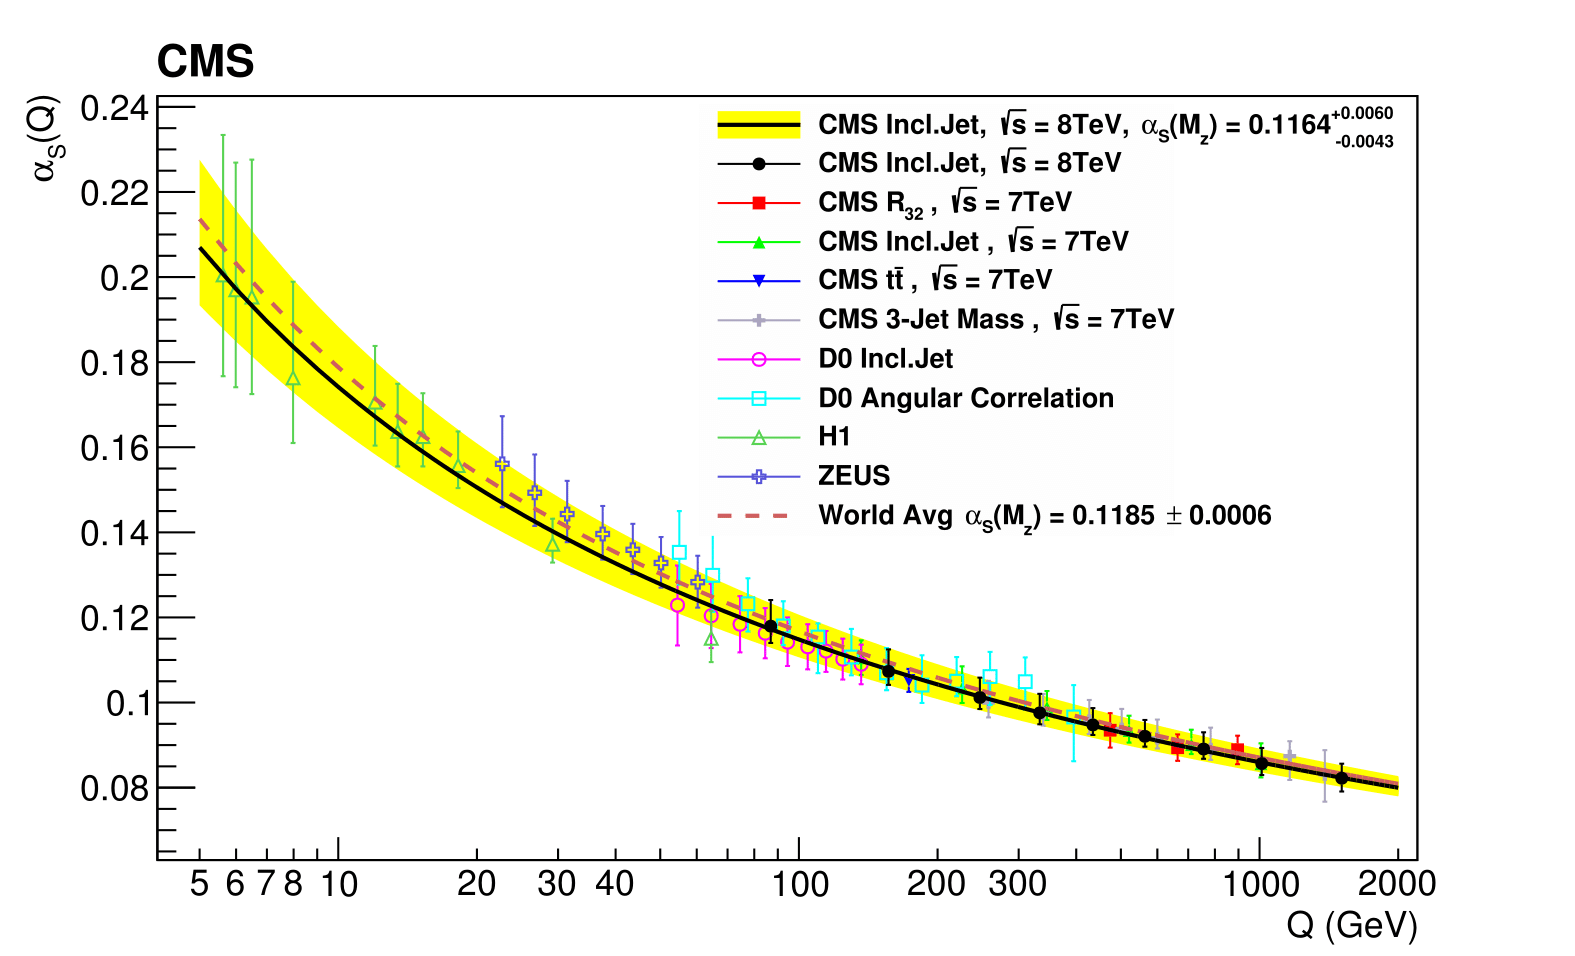
\includegraphics[width=\textwidth]{Figures/alphaS}
	\caption[The running of the strong coupling constant. At higher energy scales \alpS{} tends to 0, resulting in a strengthening of the strong force.]{The running of the strong coupling constant. At higher energy scales \alpS{} tends to 0, resulting in a strengthening of the strong force. \cite{alphaSrunning}.}
	\label{fig:alphaSrunning}
\end{figure}
At higher energies the strong coupling constant $g_{s}$ (or $\alpS = \sfrac{g_{s}^{2}}{4\pi}$) tends to 0.
This is known as asymptotic freedom and means that the strong force becomes stronger at larger quark or gluon separations.
The quarks and gluons are consequently bound in colourless states (hadrons and mesons) in a process known as \textit{colour confinement}.
Single quarks in the final state of Fig.~\ref{fig:feyn-eg} bind into baryons within a time scale of $\tau_{\mathrm{had}} \simeq \sfrac{1}{\Lambda_{\mathrm{QCD}}} \approx 3\ten{-24}\s$.
These particles can be highly energetic and if the potential energy due to the strong force confining a \qqbar{} pair is large enough then a new \qqbar{} pair will be produced from the vacuum. 
If the new daughter hadrons produced also have enough energy, the process is repeated until the confinement is strong enough to hold them together.
The splitting of hadrons and mesons in this way is known as \textit{hadronisation} and results in a spray of particles known in experimental terms as a \textit{jet}.
Similarly, when a hard interaction occurs within the colliding protons, the protons cease to become colourless states, and the remnants hadronise forming more sprays of particles.
These particles are known as the \textit{underlying event}.
The hadronisation process will be discussed in more detail in Sec.~\ref{sec:fragmentation_and_colour_reconnection}.
% subsection confinement (end)



\section{The weak interaction and electroweak unification}
\label{sec:EWK}

The weak interaction differs from \QED{} and \QCD{} in that it is possible to violate parity conservation $\Psi(x)\neq\Psi(-x)$, and to change the flavour of a quark. 
% It is also mediated by three massive gauge bosons.
Example weak interactions are highlighted in blue on Fig.~\ref{fig:feyn-ewk}.
The weak interaction is described by an $\mathrm{SU(2)}$ symmetry group, with the conserved charge being the weak isospin $T$.
The third component of weak isospin $T_{3}$, is also conserved.
Parity violation is seen in the weak interaction as only left-handed particles and right-handed anti-particles have been observed to interact via the weak force. 
% Left handed particles are particle s in which the spin directio is opposite the directio of motion
% This leads to the assumption that neutrinos are massless
\begin{figure}[h!]
\centering
\begin{tikzpicture}
\begin{feynman}
	\vertex [black!50](i1) {\(d\)};
	\vertex [right=3cm of i1](a);
	\vertex [black!50,above right=0.75cm and 1.5cm of a] (b){ISR};
	\vertex [below right=0.75cm and 1.5cm of a] (c);

	\vertex [black!50,above=2em of i1](i1a){\(u\)};
	\vertex [black!50,above=1em of i1](i1b){\(u\)};
	\vertex [right=3cm of i1a](i1ai);
	\vertex [right=3cm of i1b](i1bi);
	\vertex [above right=0.75cm and 1.5cm of i1ai] (i1aii);
	\vertex [above right=0.75cm and 1.5cm of i1bi] (i1bii);

	\vertex [right=1cm of i1a](g1);
	\vertex [right=2cm of i1a](g2);

	\vertex [black!50,below=5em of i1](i2){\(u\)};
	\vertex [right=1.5cm of i2] (d);
	\vertex [above right=0.75cm and 1.5cm of d] (e);
	\vertex [below right=0.75cm and 1.5cm of d] (f);
	\vertex [below right=0.75cm and 1.5cm of e] (g);
	\vertex [above right=0.75cm and 1.5cm of e] (h);

	\vertex [black!50,below=1em of i2](i2a){\(u\)};
	\vertex [black!50,below=2em of i2](i2b){\(d\)};
	\vertex [right=1.5cm of i2a](i2ai);
	\vertex [right=1.5cm of i2b](i2bi);
	\vertex [below right=0.75cm and 1.5cm of i2ai] (i2aii);
	\vertex [below right=0.75cm and 1.5cm of i2bi] (i2bii);

	\vertex [right=2cm of h] (i);
	\vertex [above right=1.5cm and 1.5cm of i] (j);
	\vertex [below right=1.5cm and 1.5cm of i] (k);
	\vertex [above right=1.2cm and 1.5cm of j] (j1);
	\vertex [below right=1.2cm and 1.5cm of j] (j2);
	\vertex [above right=1.2cm and 1.5cm of k] (k1);
	\vertex [below right=1.2cm and 1.5cm of k] (k2);

	\vertex [blue!50,above right=0.5cm and 1.5cm of j1] (l1){\(\ell\)};
	\vertex [blue!50,below right=0.5cm and 1.5cm of j1] (l2){\(\overline \nu_\ell\)};
	\vertex [blue!50,above right=0.5cm and 1.5cm of k1] (m1){\(q\)};
	\vertex [blue!50,below right=0.5cm and 1.5cm of k1] (m2){\(\overline q'\)};
	\vertex [black!50,above right=0.5cm and 1.5cm of k2] (o1){\(\overline b\)};
	\vertex [black!50,below right=0.5cm and 1.5cm of k2] (o2){FSR};

	\diagram* {
	(i1) -- [black!50,fermion] (a) -- [black!50,fermion, edge label=\(q\)] (h),
	(g1) -- [black!50,gluon, half left] (g2),
	(a) -- [black!50,gluon] (b),
	(i2) -- [black!50,fermion] (d) -- [black!50,gluon] (e),
	(d) -- [black!50,fermion] (f),
	(e) -- [black!50,fermion] (g),
	(h) -- [black!50,fermion, edge label=\(\overline q\)] (e),
	(h) -- [black!50,gluon] (i),
	(i) -- [blue,very thick,fermion, edge label=\(t\)] (j),
	(k) -- [blue!50,fermion, edge label=\(\overline t\)] (i),
	(j) -- [blue,very thick,boson, edge label=\(W^+\)] (j1),
	(j) -- [blue,very thick,fermion, edge label=\(b\)] (j2),
	(k) -- [blue!50,boson, edge label=\(W^-\)] (k1),
	(k2) -- [blue!50,fermion, edge label=\(\overline b\)] (k),
	(j1) -- [blue!50,fermion] (l1),
	(l2) -- [blue!50,fermion] (j1),
	(k1) -- [blue!50,fermion] (m1),
	(m2) -- [blue!50,fermion] (k1),
	(o1) -- [black!50,fermion] (k2),
	(k2) -- [black!50,gluon] (o2),
	(i1a) -- [black!50,fermion] (i1ai) -- [black!50,fermion] (i1aii),
	(i1b) -- [black!50,fermion] (i1bi) -- [black!50,fermion] (i1bii),
	(i2a) -- [black!50,fermion] (i2ai) -- [black!50,fermion] (i2aii),
	(i2b) -- [black!50,fermion] (i2bi) -- [black!50,fermion] (i2bii),
	};
\end{feynman}
\end{tikzpicture}
\caption[A Feynman diagram showing the \ttbar{} pair production and decay. An example weak interaction is shown in bold blue. Other weak interactions are shown in light blue.]{A Feynman diagram showing the \ttbar{} pair production and decay. An example weak interaction is shown in bold blue. Other weak interactions are shown in light blue.}
\label{fig:feyn-ewk}
\end{figure}
% approx 100GeV
% Y = 2(q-I3)
At higher energies, the electromagnetic and weak interactions unify into the electroweak (\EWK{}) interaction.
This combination results in a \ensuremath{\mathrm{SU(2)_{L}}\otimes\mathrm{U(1)_{Y}}} symmetry group, with three gauge fields, $W^{i}_{\mu}$, introduced by the $\mathrm{SU(2)_{L}}$ generators $\frac{1}{2}\sigma_{i}$ (the Pauli spin matrices) and one gauge field, $B_{\mu}$, from the $\mathrm{U(1)_{Y}}$ generator (weak hypercharge $Y = 2(Q-T_{3})$).
% Fermions with negative chirality (also called “left-handed” fermions) have T = 1/2, T3 pm1/2.
% Group into doublets (u, d)->(ve, e)->(1/2, -1/2)
% Behave similarly under weak interactions
% Never decays weakly into particle of the same T3.
% The corresponding anti-fermion has reversed chirality (“right-handed” antifermion) and sign reversed T3.
% Fermions with positive chirality (“right-handed” fermions) and anti-fermions with negative chirality (“left-handed” anti-fermions) have T3=0
% Form singlets that do not undergo weak interactions.
The \EWK{} gauge bosons are formed from the interferences of these fields and are formed as:
\begin{equation}
	W^{\pm}_{\mu} = \frac{1}{\sqrt{2}}(W^{1}_{\mu} \mp iW^{2}_{\mu}),
\end{equation}
\begin{equation}
	Z_{\mu} = W^{3}_{\mu}\cos{\theta_{W}} -  B_{\mu}\sin{\theta_{W}},
\end{equation}
and 
\begin{equation}
	A_{\mu} = W^{3}_{\mu}\sin{\theta_{W}} +  B_{\mu}\cos{\theta_{W}},
\end{equation}
% 4DOUG essentially four fields are created... two charged and two neutral. This fields interfere and the excitations of these inteferences give the gauge bosons.
where $\theta_{W}$ is the weak mixing angle~\cite{Th:SM1}, defined by the ratio of the two weak coupling constants (isospin and isocharge) 
\begin{equation}
	\tan(\theta_{W}) = \frac{g'}{g_{W}}.	
\end{equation}
The full \EWK{} covariant derivative and Lagrangian density are given by
\begin{equation}
D_{\mu} = \partial_{\mu}+ig_{W}\frac{\sigma_{i}}{2}W_{\mu}^{i}+ig'\frac{Y_{W}}{2}B_{\mu},
\end{equation}
and
\begin{equation}
\Lagr_{\EWK}=\overline{\Psi}i\gamma^{\mu}D_{\mu}\Psi - \frac{1}{4}B^{\mu\nu}B_{\mu\nu} - \frac{1}{4}W^{\mu\nu}_{i}W_{\mu\nu}^{i},
\end{equation}
respectively.
If this is assumed to be an accurate representation of the \EWK{} interaction, it requires that gauge bosons and fermions be massless in order to preserve the gauge symmetry.
As it is experimentally proven that fermions and the \Wboson{} and \Zboson{} bosons have mass, a solution is needed.
The problem is solved through a process called \textit{electroweak symmetry breaking}.

\subsection{Electroweak symmetry breaking} % (fold)
\label{sub:electroweak_symmetry_breaking}

Electroweak symmetry breaking solves the mass problem by keeping the particles massless but introducing a new complex scalar field doublet and potential into the Lagrangian density.
% 4 degrees of freedom - three to give mass to weak bosons
% The Higgs mechanism can be summarized by saying that the spontaneous breaking of a gauge theory by a non-zero VEV results in the disappearance of a Goldstone boson and its transformation into the longitudinal component of a massive gauge boson.
% Scalar VEV does not affect electromagnetism
% \begin{equation}
% 	\phi = 	\phi_1+i\phi_2 \\
% \end{equation}
\begin{equation}
	\phi = 
\begin{pmatrix} 
	\phi^{+} \\
	\phi^{0} \\
\end{pmatrix}
	= 
\begin{pmatrix} 
	\phi_1+i\phi_2 \\
	\phi_3+i\phi_4 \\
\end{pmatrix}
\end{equation}
\begin{equation}
\Lagr_{\mathrm{H}}=(D_{\mu}\phi)^{\dagger}(D^{\mu}\phi)-\frac{1}{2}\mu^{2}\phi^{\dagger}\phi - \frac{1}{4}\lambda(\phi^{\dagger}\phi)^{2}
\end{equation}
This potential introduces an infinite set of degenerate non-zero ground states of $\phi$.
The vacuum expectation value $v$, is the magnitude of an arbitrary ground state provided $\mu^{2}$ is negative
\begin{equation}
	v=\sqrt{-\frac{\mu^2}{\lambda}}\approx246\GeV.
\end{equation} 
The choice of $v$, conventionally along the neutral, real component of $\phi$, \textit{spontaneously} breaks the symmetry of the Lagrangian~\cite{PDG}.
The neutral component is chosen because the charged component of $\phi$ must be set to zero such that the addition of a vacuum expectation value will not break the conservation of electric charge.
By taking this choice, $\phi$ can be rewritten as a perturbation around this point
\begin{equation}
	\phi = \frac{1}{\sqrt{2}}
\begin{pmatrix} 
	0 \\
	v + H(x) \\
\end{pmatrix},
\end{equation}
where $H(x)$ is the massive \BEH{} scalar field with
\begin{equation}
	m_{H} = v\sqrt{2\lambda}.
\end{equation}
The other three degrees of freedom from the initial scalar field doublet form the three massive weak bosons, via the \BEH{} mechanism~\cite{Th:Higgs1, Th:Higgs2, Th:Higgs3} such that:
%  (\textit{Goldstone bosons})
% The longitudinal polarization components of the W and Z bosons correspond to the Goldstone bosons of the spontaneously broken part of the electroweak symmetry SU(2)⊗U(1), which, however, are not observable. 
% Because this symmetry is gauged, the three would-be Goldstone bosons are "eaten" by the three gauge bosons corresponding to the three broken generators; this gives these three gauge bosons a mass, and the associated necessary third polarization degree of freedom. This is described in the Standard Model through the Higgs mechanism.
% The Higgs mechanism is the choice of unitary gauge that 'eats' the Goldstone bosons
% Gauge symmetries do not give goldstone bosonsl they give massive bosons. Normal symmetries do.
\begin{equation}
	m_{W} = \frac{vg_{W}}{2},
	\,\,\,
	m_{Z} = \frac{v\sqrt{g_{W}^{2}+g'^{2}}}{2}.
\end{equation}
Fermions may also be permitted mass via the Higgs mechanism, by introducing additional terms to the Lagrangian density of the form 
\begin{equation} \label{eq:LY}
	\Lagr_{\mathrm{Y}} = g_{y}(\overline{\Psi}_L\phi\Psi_R+\overline{\Psi}_R\phi^{\dagger}\Psi_L), 
\end{equation}
where $g_{y}$ (\textit{Yukawa coupling}) is the coupling strength of the respective fermion to the \BEH{} field.
The Yukawa coupling strength is different for each fermion.
This leads to fermion masses which are linearly proportional to and only dependent on $g_{y}$, given by
\begin{equation}
	m_{f}=\frac{vg_{y}}{\sqrt{2}}.
\end{equation}
% subsection electroweak_symmetry_breaking (end)

\subsection{The Cabbibo-Kobayashi-Maskawa mixing matrix} % (fold)
\label{sub:the_cabbibo_kobayashi_maskawa_mixing_matrix}
The weak interaction of quarks is described by the Cabbibo-Kobayashi-Maskawa (\CKM{}) mixing matrix~\cite{Th:CKM1, Th:CKM2}.
It postulated the existence of a third family of quarks (\tquark{}, \bquark{}) to explain the observed CP violation in kaon decays~\cite{Th:CKM2}.
It relates the weak, flavour eigenstates to the mass eigenstates by
\begin{equation*}
\begin{pmatrix}
\dquark' \\
\squark' \\
\bquark'
\end{pmatrix}
=
\begin{pmatrix}
V_{\uquark\dquark} & V_{\uquark\squark} & V_{\uquark\bquark} \\
V_{\cquark\dquark} & V_{\cquark\squark} & V_{\cquark\bquark} \\
V_{\tquark\dquark} & V_{\tquark\squark} & V_{\tquark\bquark}
\end{pmatrix}
\begin{pmatrix}
\dquark \\
\squark \\
\bquark
\end{pmatrix}.
\end{equation*}
The relative strength of the weak interaction involving a flavour transition from $j\rightarrow i$ is given by the associated \CKM{} matrix element $V_{ij}$.
In the \SM{} the \CKM{} matrix is unitary ($V^{\dag}V=I$) so that each row behaves as $\abs{V_{\uquark\dquark}}^2 + \abs{V_{\uquark\squark}}^2 + \abs{V_{\uquark\bquark}}^2 = 1$.
This unitarity assumption leads to current experimental measurements of
\begin{equation*}
\begin{pmatrix}
\abs{V_{\uquark\dquark}} & \abs{V_{\uquark\squark}} & \abs{V_{\uquark\bquark}} \\
\abs{V_{\cquark\dquark}} & \abs{V_{\cquark\squark}} & \abs{V_{\cquark\bquark}} \\
\abs{V_{\tquark\dquark}} & \abs{V_{\tquark\squark}} & \abs{V_{\tquark\bquark}}
\end{pmatrix}
\approx
\begin{pmatrix}
0.974 & 0.225 & 0.004 \\
0.225 & 0.973 & 0.041 \\
0.009 & 0.040 & 0.999
\end{pmatrix},
\end{equation*}
given by~\cite{PDG}.
The relative strength of the off-diagonal \CKM{} elements means that flavour transitions between different generations of quarks are suppressed.
There is a small complex phase that is present in the $V_{\uquark\bquark}$ and $V_{\tquark\dquark}$ matrix elements, which allows for a small quantity of charge-parity (CP) violation in the \SM{}.

% Measurements senstitive to amplitude squared are not senstive to weak complex phase.
% Need measurements senstive to amplitude
% These are in neutral B and K systems.
% Use oscillations and interfereing final states.
% subsection the_cabbibo_kobayashi_maskawa_mixing_matrix (end)



\section{The standard model and its shortcomings} % (fold)
\label{sec:the_full_standard_model}
The full \SM{} combines the \QCD{} and \EWK{} field theories into the combined symmetry group \ensuremath{\mathrm{SU(3)_{c}}\otimes\mathrm{SU(2)_{L}}\otimes\mathrm{U(1)_{Y}}}.
This has the effect of making the full covariant derivative
\begin{equation}
	D_{\mu} = \partial_{\mu}+ig_{S}\frac{\lambda_{a}}{2}G_{a}+ig_{W}\frac{\sigma_{i}}{2}W_{\mu}^{i}+ig'\frac{Y_{W}}{2}B_{\mu},
\end{equation}
and the full Lagrangian density the sum of all individual components
\begin{equation}
	\Lagr_{\SM} = \Lagr_{\QCD} + \Lagr_{\EWK} + \Lagr_{\mathrm{H}} + \Lagr_{\mathrm{Y}}.
\end{equation}
It includes terms for free fermions and gauge bosons and the interactions between them, in addition to mass terms arising from the introduction of the \BEH{} field and a non-zero $v$.
It is the most complete model we have of our Universe, describing fundamental matter and its interactions to an unprecedented degree of precision, however as mentioned earlier, it is far from a complete description.
% section the_full_standard_model (end)

\subsection{Gravity} % (fold)
\label{sub:gravity}

Perhaps the largest omission from the \SM{} is the fundamental force of gravity, which all massive particles experience.
In order to include a description of gravity in the \SM{}, a unification with the theory of general relativity at the quantum scale is needed.
The formulation of this unification at present is unknown, however one popular way to do this is with string theory.
Unfortunately, the effect of gravity is completely negligible at the current accessible energy scales and as such it is not experimentally feasible to directly test any unification theory.  
% $\Lamdba_{P} \sim \ten{19} \GeV$
% subsection gravity (end)

\subsection{Massive neutrinos} % (fold)
\label{sub:massive_neutrinos}

The current observation that only left-handed neutrinos interact weakly results in the Yukawa component of the Lagrangian density shown in Eq.~\ref{eq:LY}, losing gauge invariance unless the neutrinos are massless.
Experiments such as SNO which measured a third of the number of \nue{} expected from production in the Sun~\cite{Th:SNO}, or Super-Kamiokande which measured half of the number of upward atmospheric \numu{} as downward ones~\cite{Th:SuperK}, prove an oscillation in the flavour of the neutrino.
This can be explained by the neutrinos acquiring a mass, such that the flavour states of the neutrinos are then linear superpositions of the mass states.
% Removing this statement as i don't like it - nor do i want to talk about it
% There is also no reason why right-handed neutrinos should not exist in nature.
% Goldhaber Experiment? https://indico.cern.ch/event/73981/contributions/2080329/attachments/1043729/1487656/Grodzins_Lee_Monday_Opening.pdf 
% subsection massive_neutrinos (end)

\subsection{Dark matter} % (fold)
\label{sub:dark_matter}

Other issues with the \SM{} originate from cosmological observations.
Firstly, the lack of enough mass in galaxies to explain the rotation curves of luminous matter, provides evidence for a type of additional matter which must be massive and electromagnetically inert~\cite{Th:DM1}.
This matter is known as dark matter and is predicted to contribute around 80\% to the matter content of the Universe. 
There are other cosmological indicators for dark matter including galaxy clusters~\cite{Th:DM2} and the cosmic microwave background~\cite{Th:DM3}.
While the current \SM{} does provide a set of particles which behave in this way, the neutrinos, there are not enough to account for all of the missing matter and they are too 'hot`, \ie{} their highly relativistic velocity is unable to explain observations.

The second issue is that the observation of the accelerating expansion of the Universe implies that there is a repulsive operation acting~\cite{Th:DM4}.
This process is enshrined under the term dark energy, which accounts for 70\% of the mass-energy content of the Universe.
The \SM{} has no mechanism for describing dark energy.
% Clusters: Viral theorem (essentially roation curve again) and lensing 
% CMB: anisotropy can be mapped to power law spectrum. three peaks.. 3rd relates to DM.
% subsection dark_matter (end)

\subsection{Baryon asymmetry} % (fold)
\label{sub:baryon_asymmetry}

Another striking problem in the \SM{} is the matter-antimatter imbalance seen in the Universe.
The Universe is predominantly matter based, however the \SM{} predicts that matter and antimatter are produced in equal quantities.
Somehow, the antimatter present at the beginning of the Universe has been transformed or destroyed and therefore a process is required which favours matter over anti-matter~\cite{Th:BaryonAsym}.
While the \SM{} does provide an explanation for some of this transformation in the lepton sector, from the CP violating, complex phases of the quark and neutrino mixing matrices, it contributes negligible amounts to the imbalance seen.

% (factor of $\sim10^{-20}$).

% The reference~\cite{Th:BaryonAsym} also displays some of the candidate theories to explain the imbalance
% elctroweak baryogenesis
% leptogenesis - seesaw
% Transformed into matter? or dark matter? maybe antimatter couples more stronly to dark matter?
% page 13 of ref
% subsection baryon_asymmetry (end)


\subsection{Hierarchy problem} % (fold)
\label{sub:hierarchy_problem}

The mass of the \Hboson{} boson depends on its bare mass and corrections from fermion loops depending on the square of the energy scale $\Lambda$.
\begin{equation*}
	m_{\mathrm{H}}^{2} = m_{\mathrm{H, bare}}^{2} + \mathcal{O}(\Lambda^{2})
\end{equation*}
At the \EWK{} scale ($100\GeV$), these quantum loop corrections are small, however as the energy scale approaches the Planck scale ($10^{19}\GeV$), the point at which the \SM{} is no longer valid, the corrections diverge.
The very large divergences must be cancelled to keep the observed \Hboson{} boson mass light.
This requires a significant amount of fine-tuning in the \SM{}.
% 100GeV, 10^19 GeV?
One way this unnatural amount of fine-tuning can be alleviated, is to introduce an additional set of particles which, in part, cancel the loop corrections.
\textit{Supersymmetry} is one example of a theory that creates an additional set of particles by creating a symmetry of spin in the \SM{}~\cite{Th:SUSY}.
For every \SM{} particle there exists a massive supersymmetric particle, differing by a half unit of spin, which can be present in quantum loop corrections to the \Hboson{} boson mass at higher energy scales, cancelling contributions from the \SM{} particles.
% They have opposite sign contributions.

% subsection hierarchy_problem (end)

% section shortcomings_of_the_standard_model (end)




\section{Top quark physics} % (fold)
\label{sec:top_quark_physics}

% The first evidence for the top quark was seen by the CDF experiment at the Tevatron in 1994, and its discovery published in 1995 from a combination of the results from both the CDF and D0 experiments~\cite{Th:TopCDF,Th:TopD0}.
The discovery of the top quark was published in 1995 from a combination of the results from both the CDF and D0 experiments~\cite{Th:TopCDF,Th:TopD0}.
It is the most massive particle in the SM to date, at 172.5\GeV{}.
The large mass means that the lifetime of the top quark is very short at $\tau_{\mathrm{t}} = \sfrac{1}{\Gamma_{\mathrm{t}}} \simeq 5\ten{-25}\s$~\cite{PDG}.
In fact, it is shorter than the typical time it takes for a quark to hadronise, $\tau_{\mathrm{had}} \approx 3\ten{-24}\s$ so that it is possible for the bare quark properties to be measured directly.

Now, at the LHC, more top quarks are being produced than ever before, leading to a vast array of measurements being performed, such as precision measurements of the \SM{}, searches for rare \SM{} processes and searches for possible new physics present in top quark decays.
Not only is top quark physics important in direct searches for new physics, it is often the process which forms the largest background in other searches for particles beyond the \SM{}.
Therefore, it is crucial to know the production cross section of the top quark as precisely as possible.
The precise top quark production cross section measurements can also uniquely be used to directly probe the $V_{tb}$ element of the CKM matrix ($V_{tb} >> V_{ts} > V_{td}$), to set constraints on the gluon and quark \textit{parton distribution functions} (PDFs) at high $M(\ttbar)$ and to measure the top quark Yukawa coupling strength.
% This is important as the top quark Yukawa coupling provides the largest correction to the mass of the \Hboson{} boson and TODO
% Define CDS
% Top Yukawa ~1 : Much larger hierarchy

\subsection{Top quark production} % (fold)
\label{sub:top_quark_production}

Protons are made up of three valence quarks (\uquark{}\uquark{}\dquark{}), confined by gluons. 
At higher energies, the gluon multiplicity increases, as well as the number of pair-produced \qqbar{} pairs, known as sea quarks.
This means that it is much more probable that an interaction will occur from collisions between gluons or non-valence quarks.
Top quark production at the LHC at \com{} proceeds primarily via \ttbar{} pair-production, where $\sim90\%$ is from gluon-gluon fusion. 
The further $\sim10\%$ comes from quark-antiquark annihilation.
The quark-antiquark production mode is shown in Fig.~\ref{fig:feyn-eg}. 
The top quark can also be produced singly via the s- and t- channels and in association with a \Wboson{} boson, as shown in Fig.~\ref{fig:feyn-t}.
The production cross section for single top quarks is much smaller than that for \ttbar{} production because of the composition of the initial states required.
Higher top multiplicity final states are also available in the \SM{} but with a much smaller production cross section~\cite{Gen:MGamc}.
% or as a quadruplet, as shown in Fig.~\ref{fig:feyn-tttt}.
% Measurements of single top production are especially interesting as the cross section is directly proportional to the $|V_{tb}|$ matrix element (assuming $|V_{tb}| >> |V_{ts}| > |V_{td}|$)
% Add tttt as an example?
% Add Vtb and top spin?
\begin{figure}[h!]
	\centering
	\begin{subfigure}{.32\textwidth}
		\centering
		\begin{tikzpicture}
		\begin{feynman}
			\vertex (A);
			\vertex [above left=0.75cm and 1.5cm of A] (ai) {\(\overline{q}'\)};
			\vertex [below left=0.75cm and 1.5cm of A] (aii) {\(q\)};

			\vertex [right=1.5cm of A] (B);
			\vertex [above right=0.75cm and 1.5cm of B] (bi) {\(t\)};
			\vertex [below right=0.75cm and 1.5cm of B] (bii) {\(\overline{b}\)};

			\diagram*{
			(ai) -- [anti fermion] (A),
			(aii) -- [fermion] (A),
			(A) -- [boson, edge label=\(W^{+}\)] (B),
			(B) -- [fermion] (bi),
			(B) -- [anti fermion] (bii),
			};
		\end{feynman}
		\end{tikzpicture}
	\end{subfigure}
	\begin{subfigure}{.32\textwidth}
		\centering
		\begin{tikzpicture}
		\begin{feynman}
			\vertex [black](i1){\(q\)};
			\vertex [black,right=1.5cm of i1](a);
			\vertex [black,above right=0.75cm and 1.5cm of a](f1){\(q'\)};
			\vertex [black,below right=0.75cm and 1.5cm of a](b);
			\vertex [black,right=1.5cm of b](f2){\(t\)};
			\vertex [black,below=1.5cm of i1](i2){\(g\)};
			\vertex [black,right=1.5cm of i2](c);
			\vertex [black,below right=0.75cm and 1.5cm of c] (f3){\(\overline{b}\)};

			\diagram* {
			(i1) -- [black,fermion] (a) -- [black,fermion] (f1),
			(a) -- [black,boson, edge label=\(W^{+}\)] (b),
			(i2) -- [black,gluon] (c),
			(c) -- [black,fermion] (b),
			(b) -- [black,fermion] (f2),
			(c) -- [black,anti fermion] (f3),
			};
		\end{feynman}
		\end{tikzpicture}
	\end{subfigure}
	\begin{subfigure}{.32\textwidth}
		\centering
		\begin{tikzpicture}
		\begin{feynman}
			\vertex [black](i1){\(g\)};
			\vertex [black,right=1.5cm of i1](a);
			\vertex [black,above right=0.75cm and 1.5cm of a](f1){\(t\)};
			\vertex [black,below right=0.75cm and 1.5cm of a](b);
			\vertex [black,right=1.5cm of b](f2){\(W^{-}\)};
			\vertex [black,below=1.5cm of i1](i2){\(g\)};
			\vertex [black,right=1.5cm of i2](c);
			\vertex [black,below right=0.75cm and 1.5cm of c] (f3){\(\overline{b}\)};

			\diagram* {
			(i1) -- [black,gluon] (a)
			(a) -- [black,fermion] (f1),
			(a) -- [black,anti fermion] (b),
			(b) -- [black,boson] (f2),
			(i2) -- [black,gluon] (c),
			(c) -- [black,fermion] (b),
			(c) -- [black,anti fermion] (f3),
			};
		\end{feynman}
		\end{tikzpicture}
	\end{subfigure}
	\caption[Feynman diagrams for the production of single top quarks. On the left, via the s-channel, in the middle via the t-channel and on the right via the tW channel.]{Feynman diagrams for the production of single top quarks. On the left, via the s-channel, in the middle via the t-channel and on the right via the tW channel. }
	\label{fig:feyn-t}
\end{figure}
% \begin{figure}[h!]
	\centering
	\begin{subfigure}{.49\textwidth}
		\centering
		\begin{tikzpicture}
		\begin{feynman}
			\vertex [black](i1){\(g\)};
			\vertex [black,right=1.5cm of i1](a);
			\vertex [black,above right=0.75cm and 1.5cm of a](f1){\(t\)};
			\vertex [black,below right=0.75cm and 1.5cm of a](b);
			\vertex [black,right=1.5cm of b](f2);
			\vertex [black,above right=0.75cm and 1.5cm of f2](f2a){\(t\)};
			\vertex [black,below right=0.75cm and 1.5cm of f2](f2b){\(\overline{t}\)};
			\vertex [black,below=1.5cm of i1](i2){\(g\)};
			\vertex [black,right=1.5cm of i2](c);
			\vertex [black,below right=0.75cm and 1.5cm of c] (f3){\(\overline{t}\)};

			\diagram* {
			(i1) -- [black,gluon] (a)
			(a) -- [black,fermion] (f1),
			(a) -- [black,anti fermion] (b),
			(b) -- [black,gluon] (f2),
			(f2) -- [black,fermion] (f2a),
			(f2) -- [black,anti fermion] (f2b),
			(i2) -- [black,gluon] (c),
			(c) -- [black,fermion] (b),
			(c) -- [black,anti fermion] (f3),
			};
		\end{feynman}
		\end{tikzpicture}
	\end{subfigure}
	\begin{subfigure}{.49\textwidth}
		\centering
		\begin{tikzpicture}
		\begin{feynman}
			\vertex [black](i1){\(g\)};
			\vertex [black,right=1.5cm of i1](a);
			\vertex [black,above right=0.75cm and 1.5cm of a](f1){\(\overline{t}\)};
			\vertex [black,below right=0.75cm and 1.5cm of a](c);
			\vertex [black,above right=0.75cm and 1.5cm of b](f2){\(t\)};

			\vertex [black,below=2.5cm of i1](i2){\(g\)};
			\vertex [black,right=1.5cm of i2](b);
			\vertex [black,above right=0.75cm and 1.5cm of b](d);
			\vertex [black,below right=0.75cm and 1.5cm of b](f3){\(t\)};
			\vertex [black,below right=0.75cm and 1.5cm of d](f4){\(\overline{t}\)};

			\diagram* {
			(i1) -- [black,gluon] (a)
			(a) -- [black,anti fermion] (f1),
			(a) -- [black,fermion] (c),
			(c) -- [black,fermion] (f2),
			
			(c) -- [black,gluon] (d),

			(i2) -- [black,gluon] (b)
			(b) -- [black,fermion] (f3),
			(b) -- [black,anti fermion] (d),
			(d) -- [black,anti fermion] (f4),
			};
		\end{feynman}
		\end{tikzpicture}
	\end{subfigure}
	\caption[Feynman diagrams for the production of four top quarks. The mediating boson is predominantly a gluon, however photons, \Zboson{} bosons and \Hboson{} bosons can also mediate.]{Feynman diagrams for the production of four top quarks. The mediating boson is predominantly a gluon, however photons, \Zboson{} bosons and \Hboson{} bosons can also mediate. }
	\label{fig:feyn-tttt}
\end{figure}

The production cross section for the interaction $\sigma_{pp\to\ttbar{}}$, is predicted by the convolution of the partonic cross section $\hat{\sigma}_{\ttbar{}}$ derived directly from the Feynman diagrams and the PDFs of the incident protons $f(x, \mu^{2})$, summed over all possible parton flavours.
This is given by
\begin{equation}
\label{eq:pdf}
	\sigma_{pp\to\ttbar{}} = \sum_{a, b}\int_{0}^{1}f(x_{a}, \mu^{2})dx_{a}\,\,.\,\int_{0}^{1}f(x_{b}, \mu^{2})dx_{b}\,\,.\,\,\hat{\sigma}_{ab\to\ttbar{}}.
\end{equation}
The parton distribution function is defined as the number density of a parton carrying a fraction $x$ of the total momentum of the proton in the longitudinal direction at the energy scale being probed, $\mu$.
The \PDF{}s are measured from global fits to many different data measurements and sources, such as measurements of deep inelastic scattering, Drell-Yan production, \ttbar{} production and inclusive jet production, from many experiments at colliders such as Hadron-Electron Ring Accelerator and the LHC.
The \PDF{} is calculated at some arbitrary $\mu^{2} = \mu^{2}_{0}$, which is taken as 1\GeV{} by the $\mathrm{NNPDF}$ collaboration in the $\mathrm{NNPDF3.1}$ \PDF{} set~\cite{NNPDF3p1}.
This is then evolved through the Dokshitzer-Gribov-Lipatov-Altarelli-Parisi (DGLAP) equations~\cite{Th:D, Th:GL, Th:AP} to higher energy scales.
The $xf(x, \mu^{2})$ distributions for the $\mathrm{NNPDF3.1}$ \PDF{} set at $\mu^{2} = 10\GeVsq$ and $\mu^{2} = 10^{4}\GeVsq$ are displayed in Fig.~\ref{fig:pdf}.
When moving from low to high $\mu^{2}$ values, it is clearly seen that a greater fraction of the momentum of the proton is carried by an increasing number of non-valence partons.
\begin{figure}[htpb]
	\centering
	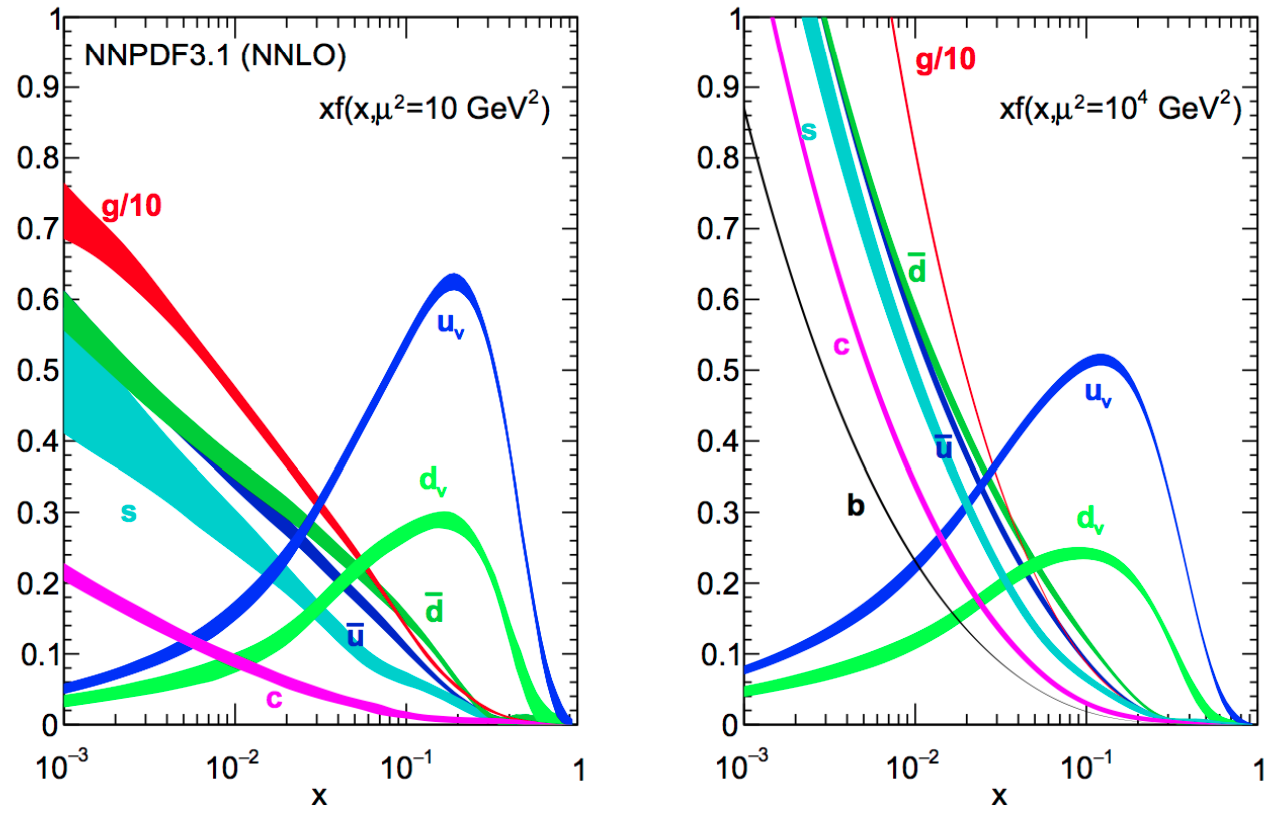
\includegraphics[width=0.9\textwidth]{Figures/PDF}
	\caption[The parton distribution function of the proton scaled by the fraction of momentum carried by the parton, $xf(x, \mu^2)$ with respect to the fraction of momentum carried by the parton. The left panel shows the distributions with respect to a lower energy scale and the right panel with respect to a higher energy scale.]{ The parton distribution function of the proton scaled by the fraction of momentum carried by the parton, $xf(x, \mu^2)$ with respect to the fraction of momentum carried by the parton. The left panel shows the distributions with respect to a lower energy scale and the right panel with respect to a higher energy scale~\cite{NNPDF3p1}. }
	\label{fig:pdf}
\end{figure}

The prediction of the inclusive \ttbar{} cross section from proton-proton collisions is shown in Fig.~\ref{fig:incttbar}, together with current experimental measurements. 
The prediction from proton-anti-proton collisions is also shown.
The cross sections converge at higher energies due to the increase in collisions between non-valence partons the distribution of which is identical in protons and anti-protons.
At \com{}, the inclusive \ttbar{} production cross section was calculated to be $831.8^{+19.8}_{-29.2}(\text{scale})\pm35.1(\text{PDF}+\alpS)\pb$~\cite{TOPpp}.
This \ttbar{} cross section is calculated to next-to-next-to-leading-order (\NNLO{}) accuracy in perturbative \QCD{}, including resummation of next-to-next-to-leading logarithmic soft-gluon terms with \textsc{Top++} (v2.0)~\cite{Th:XSEC1,Th:XSEC2,Th:XSEC3,Th:XSEC4,Th:XSEC5,Th:XSEC6,Th:XSEC7}.
% TODO ADD MORE?
% The scale uncertainty in this \ttbar{} cross section comes from the independent variation of the factorization and renormalization scales.
\begin{figure}[htpb]
	\centering
	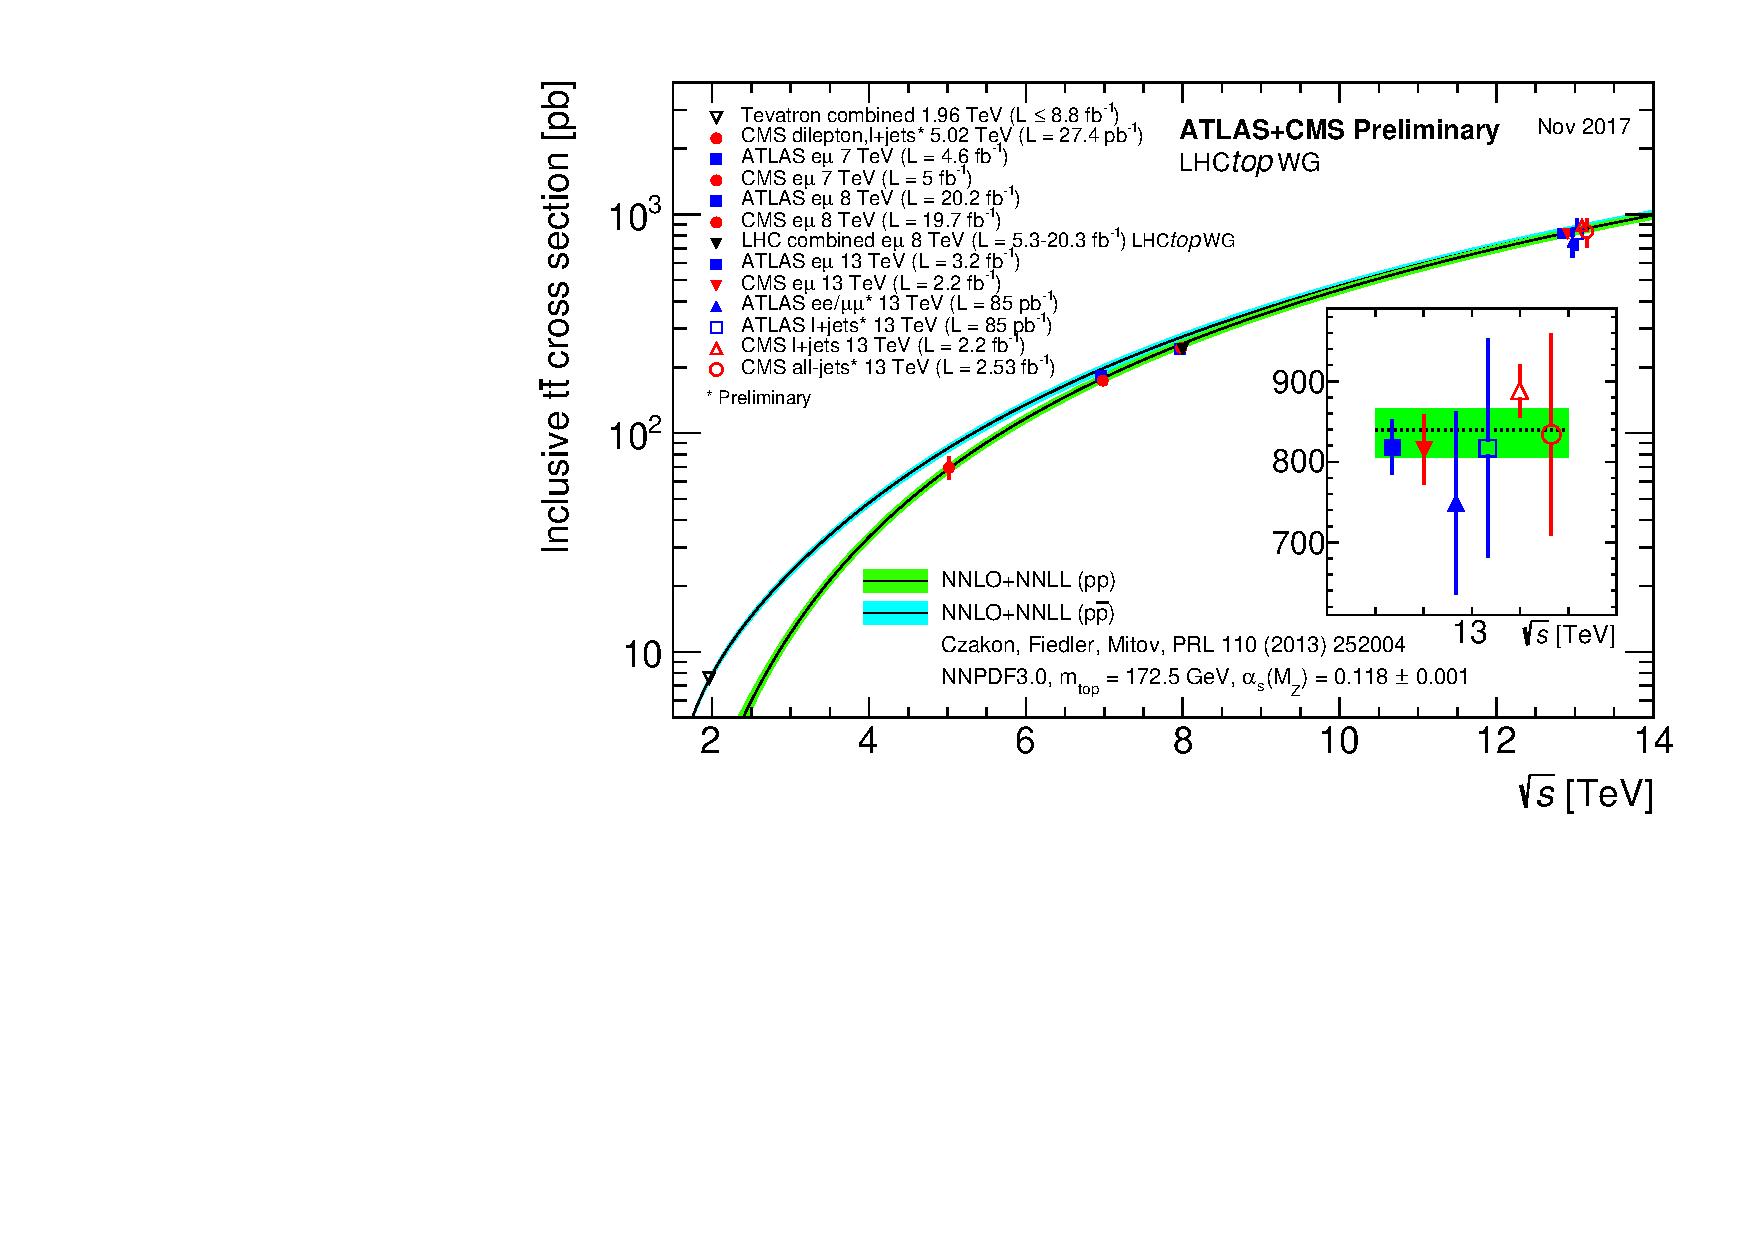
\includegraphics[width=0.9\textwidth]{Figures/tt_curve_sqrts_cms}
	\caption[The inclusive \ttbar cross section, measured by ATLAS, CMS and the Tevatron in different decay channels at multiple \sqrts{}. Also shown is the most precise theoretical prediction to date.]{ The inclusive \ttbar cross section, measured by ATLAS, CMS and the Tevatron in different decay channels at multiple \sqrts{}. Also shown is the most precise theoretical prediction to date~\cite{LHCTopWG_Plots}. }
	\label{fig:incttbar}
\end{figure}
% subsection top_quark_production (end)

\subsection{Order of perturbation} % (fold)
\label{sub:order_of_perturbation}

The cross section of a process depends on a quantity known as the \textit{matrix element}
\begin{equation*}
	\hat{\sigma}_{\ttbar{}}\propto\abs{\mathcal{M}}^2
\end{equation*}
and the matrix element can be calculated using the Feynman rules from Feynman diagrams.
Increasing the order of perturbation essentially adds an additional parton to each diagram which makes the matrix-element calculation much more complex but gives increasing accuracy.
A comparison of the Feynman diagrams at leading order (\LO{}) and next-to-leading order (\NLO{}) is shown in Fig.~\ref{fig:feyn-nlo}, where in the top left panel a simple \LO{} tree-diagram is shown. 
The top right panel shows loops in the propagator which can be related to the running of \alpS{}.
The rest of the panels show \NLO{} processes, where the centre two panels are displaying loops corresponding to virtual particles 
% whose properties counteract the infra-red divergences introduced by the radiation of soft collinear partons of the form seen in the lower two panels.
and the lower two panels contribute real partons to the final state.
\begin{figure}
\centering
\begin{resizedtikzpicture}{0.45\linewidth}
\begin{feynman}
	\vertex (A);
	\vertex [below=3cm of A](B);
	\vertex [below right=1.5cm and 3cm of A](C);

	\vertex [right=1cm of C](D1);
	\vertex [right=2cm of C](D2);
	\vertex [right=3cm of C](D3);
	\vertex [above right=0.375cm and 0.75cm of D3] (E1);
	\vertex [above right=0.75cm and 1.5cm of D3] (E2);
	\vertex [above right=1.5cm and 3cm of D3] (E3);
	\vertex [above right=0.375cm and 0.75cm of D3] (F1);
	\vertex [below right=0.75cm and 1.5cm of D3] (F2);
	\vertex [below right=1.5cm and 3cm of D3] (F3);

	\diagram* {
	(A) -- [fermion] (C),
	(B) -- [anti fermion] (C),

	(C) -- [gluon] (D3),
	(D3) -- [fermion] (E3),
	(D3) -- [anti fermion] (F3),
	};
\end{feynman}
\end{resizedtikzpicture} \\
\caption[A Feynman diagram showing a \LO{} process.]{A Feynman diagram showing a \LO{} process.}
\label{fig:feyn-nlo1}
\end{figure}

\begin{figure}
\centering
\begin{resizedtikzpicture}{0.45\linewidth}
\begin{feynman}
	\vertex (A);
	\vertex [below=3cm of A](B);
	\vertex [below right=1.5cm and 3cm of A](C);

	\vertex [right=1cm of C](D1);
	\vertex [right=2cm of C](D2);
	\vertex [right=3cm of C](D3);
	\vertex [above right=0.375cm and 0.75cm of D3] (E1);
	\vertex [above right=0.75cm and 1.5cm of D3] (E2);
	\vertex [above right=1.5cm and 3cm of D3] (E3);
	\vertex [above right=0.375cm and 0.75cm of D3] (F1);
	\vertex [below right=0.75cm and 1.5cm of D3] (F2);
	\vertex [below right=1.5cm and 3cm of D3] (F3);

	\diagram* {
	(A) -- [fermion] (C),
	(B) -- [anti fermion] (C),

	(C) -- [gluon] (D3),
	(D3) -- [fermion] (E3),
	(D3) -- [anti fermion] (F3),
	(D2) -- [gluon, half left] (E1),
	};
\end{feynman}
\end{resizedtikzpicture}
\hspace{1cm}
\begin{resizedtikzpicture}{0.45\linewidth}
\begin{feynman}
	\vertex (A);
	\vertex [below=3cm of A](B);
	\vertex [below right=1.5cm and 3cm of A](C);

	\vertex [right=1cm of C](D1);
	\vertex [right=2cm of C](D2);
	\vertex [right=3cm of C](D3);
	\vertex [above right=0.375cm and 0.75cm of D3] (E1);
	\vertex [above right=0.75cm and 1.5cm of D3] (E2);
	\vertex [above right=1.5cm and 3cm of D3] (E3);
	\vertex [above right=0.375cm and 0.75cm of D3] (F1);
	\vertex [below right=0.75cm and 1.5cm of D3] (F2);
	\vertex [below right=1.5cm and 3cm of D3] (F3);

	\diagram* {
	(A) -- [fermion] (C),
	(B) -- [anti fermion] (C),

	(C) -- [gluon] (D3),
	(D3) -- [fermion] (E3),
	(D3) -- [anti fermion] (F3),
	(E2) -- [gluon, half left] (F2),
	};
\end{feynman}
\end{resizedtikzpicture} \\
\vspace{0.5cm}
\begin{resizedtikzpicture}{0.45\linewidth}
\begin{feynman}
	\vertex (A);
	\vertex [below=3cm of A](B);
	\vertex [below right=1.5cm and 3cm of A](C);
	\vertex [below right=0.75cm and 1.5cm of A](A1);
	\vertex [above right=0.75cm and 1.5cm of A1](A2);

	\vertex [right=1cm of C](D1);
	\vertex [right=2cm of C](D2);
	\vertex [right=3cm of C](D3);
	\vertex [above right=0.375cm and 0.75cm of D3] (E1);
	\vertex [above right=0.75cm and 1.5cm of D3] (E2);
	\vertex [above right=1.5cm and 3cm of D3] (E3);
	\vertex [above right=0.375cm and 0.75cm of D3] (F1);
	\vertex [below right=0.75cm and 1.5cm of D3] (F2);
	\vertex [below right=1.5cm and 3cm of D3] (F3);
	\vertex [below right=0.75cm and 1.5cm of E2] (G);

	\diagram* {
	(A) -- [fermion] (C),
	(B) -- [anti fermion] (C),

	(C) -- [gluon] (D1),
	(D1) -- [gluon, half left] (D2),
	(D2) -- [gluon, half left] (D1),
	(D2) -- [gluon] (D3),
	(D3) -- [fermion] (E3),
	(D3) -- [anti fermion] (F3),
	};
\end{feynman}
\end{resizedtikzpicture} \\
\caption[A set of Feynman diagrams showing virtual \NLO processes. These loops are responsible for the running of the strong coupling constant.]{A set of Feynman diagrams showing virtual \NLO processes. These loops are responsible for the running of the strong coupling constant.}
\label{fig:feyn-nlo2}
\end{figure}

\begin{figure}
\centering
\begin{resizedtikzpicture}{0.45\linewidth}
\begin{feynman}
	\vertex (A);
	\vertex [below=3cm of A](B);
	\vertex [below right=1.5cm and 3cm of A](C);
	\vertex [below right=0.75cm and 1.5cm of A](A1);
	\vertex [above right=0.75cm and 1.5cm of A1](A2);

	\vertex [right=1cm of C](D1);
	\vertex [right=2cm of C](D2);
	\vertex [right=3cm of C](D3);
	\vertex [above right=0.375cm and 0.75cm of D3] (E1);
	\vertex [above right=0.75cm and 1.5cm of D3] (E2);
	\vertex [above right=1.5cm and 3cm of D3] (E3);
	\vertex [above right=0.375cm and 0.75cm of D3] (F1);
	\vertex [below right=0.75cm and 1.5cm of D3] (F2);
	\vertex [below right=1.5cm and 3cm of D3] (F3);

	\diagram* {
	(A) -- [fermion] (C),
	(B) -- [anti fermion] (C),

	(C) -- [gluon] (D3),
	(D3) -- [fermion] (E3),
	(D3) -- [anti fermion] (F3),
	(A1) -- [gluon] (A2),
	};
\end{feynman}
\end{resizedtikzpicture}
\hspace{1cm}
\begin{resizedtikzpicture}{0.45\linewidth}
\begin{feynman}
	\vertex (A);
	\vertex [below=3cm of A](B);
	\vertex [below right=1.5cm and 3cm of A](C);
	\vertex [below right=0.75cm and 1.5cm of A](A1);
	\vertex [above right=0.75cm and 1.5cm of A1](A2);

	\vertex [right=1cm of C](D1);
	\vertex [right=2cm of C](D2);
	\vertex [right=3cm of C](D3);
	\vertex [above right=0.375cm and 0.75cm of D3] (E1);
	\vertex [above right=0.75cm and 1.5cm of D3] (E2);
	\vertex [above right=1.5cm and 3cm of D3] (E3);
	\vertex [above right=0.375cm and 0.75cm of D3] (F1);
	\vertex [below right=0.75cm and 1.5cm of D3] (F2);
	\vertex [below right=1.5cm and 3cm of D3] (F3);
	\vertex [below right=0.75cm and 1.5cm of E2] (G);

	\diagram* {
	(A) -- [fermion] (C),
	(B) -- [anti fermion] (C),

	(C) -- [gluon] (D3),
	(D3) -- [fermion] (E3),
	(D3) -- [anti fermion] (F3),
	(E2) -- [gluon] (G),
	};
\end{feynman}
\end{resizedtikzpicture} \\
\caption[A set of Feynman diagrams showing real \NLO{} processes. These are represented by the emission of real additional partons that can be seen in the final state.]{A set of Feynman diagrams showing real \NLO{} processes. These are represented by the emission of real additional partons that can be seen in the final state.}
\label{fig:feyn-nlo3}
\end{figure}
% \caption[A set of Feynman diagrams showing \LO{} and \NLO{} processes. In the top left panel, the leading order diagram is shown. The top right panel shows a gluon-loop in the propagator. These loops are responsible for the running strong coupling constant. The two middle panels show \NLO loops providing virtual particles to the diagrams and corrections in the renormalisation scale. Finally, the bottom two panels show the real additional partons that can be seen in the final state due to \NLO{} matrix-element calculations.]{A set of Feynman diagrams showing \LO{} and \NLO{} processes. In the top left panel, the leading order diagram is shown. The top right panel shows a gluon-loop in the propagator. These loops are responsible for the running strong coupling constant. The two middle panels show \NLO loops providing virtual particles to the diagrams and corrections in the renormalisation scale. Finally, the bottom two panels show the real additional partons that can be seen in the final state due to \NLO{} matrix-element calculations.}

Perturbation theory is valid at high energy scales, however at lower energy scales \QCD{} production becomes non-perturbative and the cross section is not able to be calculated using the matrix-element.
The method of dealing with non-perturbative \QCD{} is dealt with in Sec.~\ref{sec:additional_interactions_and_soft_processes}.

% Perturbation theory is valid at high energy scales, however when calculating including contributions at a much softer scale, see Section TODO, \alpS{} is accompanied by large logarithms of the ratio of the two scales.
% When approaching the edge of phase space close to the lower energy scale, such that the real emissions from soft gluons are neglected, but the virtual contributions still exist, these large logarithms are no longer cancelled.
% This leads to divergences in the partonic cross section in this area of phase space and so a soft gluon resummation must be applied.

% subsection order_of_perturbation (end)


\subsection{Top quark decay} % (fold)
\label{sub:top_quark_decay}

In the \SM{}, the top quark will decay 99.9\%~\cite{PDG} of the time to a \bquark{} quark and \Wboson{} boson.
The \Wboson{} boson then subsequently decays either into a \qpqbar{} pair (hadronic) or a \lepton{}\neutrinobar{} pair (leptonic).
In the case of \ttbar{} production, this leads to three classes of final states, the first where both \Wboson{} bosons decay leptonically, the second where both decay  hadronically and lastly where one decays leptonically and the other hadronically.
These are known as the \textit{dilepton}, \textit{all-hadronic} and \textit{single lepton} decay channels respectively.
The probability of decaying to a specific final state (\textit{branching ratio}) is approximately $10\%$ for the dilepton channel and $45\%$ for the hadronic and single lepton channels.
% W->(ud*3, cs*3, enu, munu, taunu) us cd suppressed

Each final state category has merits and drawbacks for use in analyses. 
The dilepton final state provides the most clean experimental signature, however this comes at the cost of a reduced branching ratio.
It is difficult to fully reconstruct the whole event as both neutrinos contribute to the missing transverse momentum.
The all-hadronic final state in comparison has a large branching ratio and a large multijet \QCD{} background.
The high jet multiplicity can also cause problems from the combinatorics when reconstructing the \ttbar{} system.
While the all-hadronic final state is difficult at lower collision energies, it gains in sensitivity when analysed at high collision energies.
This is because the decay products of the top quark collimate and merge into a single jet, which is able to be tagged as coming from a top quark, through jet-substructure techniques.
Finally the single lepton decay channel has a large branching ratio, but with much reduced backgrounds with respect to the all-hadronic final state. 
The final states in which a tau particle is produced are often neglected however, due to the added complexity of reconstructing them.
More details about the reconstruction of particles can be found in Ch.~\ref{ch:ObjectReconstruction}.
% For this reason \lepton{} will be used to refer to just \electron{} and \muon{}.
% subsection tt_decay (end)

\subsection{Top quark cross section measurements} % (fold)
\label{sub:top_quark_cross_section_measurements}

Figure.~\ref{fig:incttbar} shows, in addition to the theoretical prediction of the inclusive \ttbar{} production cross section, the corresponding experimental measurements, from both the CMS and A Toriodal Large ApparatuS (ATLAS) at different centre-of-mass energies (\sqrts{}) in all of the channels previously stated.
At CMS, the inclusive \ttbar{} cross section measurements are performed at 13\TeV{}~\cite{TOP16005, TOP16006} at 7 and 8 \TeV{}~\cite{TOP10001, TOP10002, TOP10003, TOP11002, TOP11003, TOP11004, TOP11005, TOP12007, TOP12026, TOP12041, TOP13004, TOP14018} and at 5\TeV{}~\cite{TOP16023}.
Inclusive cross section measurements have been performed for \ttbar{} production in association with a photon~\cite{TOP14008}, vector boson~\cite{TOP17005} and most recently \Hboson{} boson~\cite{HIG17035}.

Measurements of the \ttbar{} production cross section with respect to some other variable are known as \textit{differential} cross section measurements.
Differential cross section measurements are especially useful for testing the understanding of state-of-the-art theoretical models.
Ideally, these models should describe \ttbar{} production with respect to all kinematic variables accurately, including contributions from additional jets, and should do so for all \sqrts{}.
In practice this is not the case, with the \ttbar{} models being \textit{tuned} to best describe the kinematic distributions.
A tune is a complete set of simulation parameters describing physics processes within the simulation of the model, which have been varied to best describe differential data distributions.
Figure.~\ref{fig:8TeVTuning} shows the effect of this tuning on a set of \ttbar{} models, where the new tune is shown in solid and the old in dashed, when comparing the cross sections as a function of the magnitude of the transverse momentum of the hadronically decaying top quark, \ptToph{}, and the additional jet multiplicity.
It is worth noting, that a tune applied to a specific model may not describe the differential data better than when applied to another independent model.
The different models behind \ttbar{} production are explained in more detail in Ch.~\ref{ch:MC}.
Indeed by changing the tune, it may cause the same model to describe some kinematic distributions to a worse degree, while improving other parts of the phase space.
\begin{figure}[htpb]
	\centering
	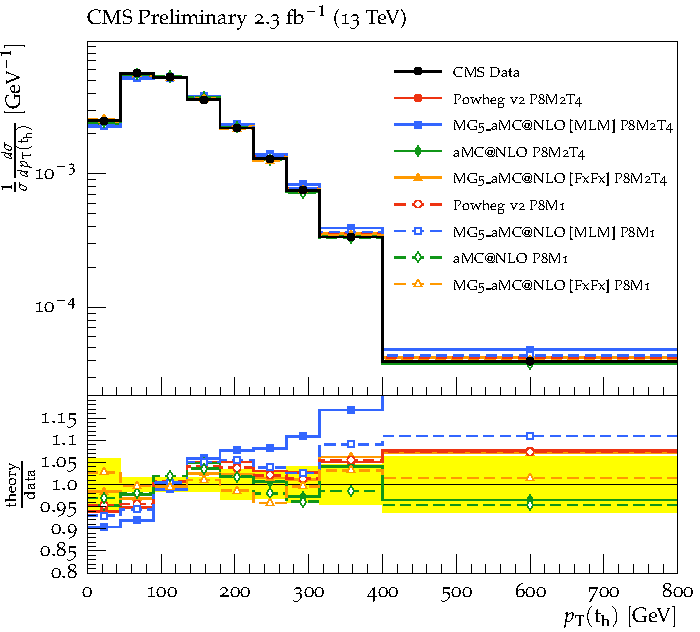
\includegraphics[width=0.49\textwidth]{Figures/TuningEx3}
	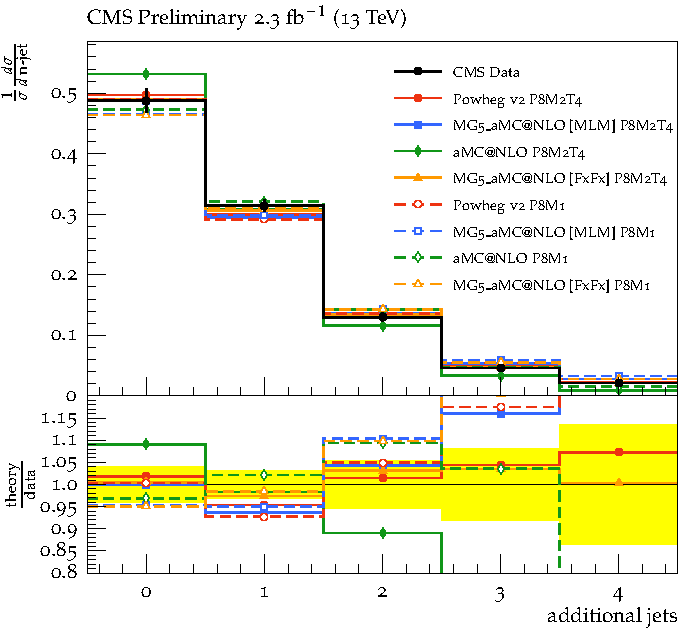
\includegraphics[width=0.49\textwidth]{Figures/TuningEx2}
	\caption[Comparison of different \ttbar{} models with the old \CUETold{} tune, represented by dashed lines, and the new \CUET{} tune, given by solid lines. The left panel shows the comparison for the distribution of the \pt{} of the hadronically decaying top quark and the right panel for the additional jets distribution.]{ Comparison of different \ttbar{} models with the old \CUETold{} tune, represented by dashed lines, and the new \CUET{} tune, given by solid lines. The left panel shows the comparison for the distribution of the \pt{} of the hadronically decaying top quark and the right panel for the additional jets distribution~\cite{Gen:CUETP8M2T4}. }
	\label{fig:8TeVTuning}
\end{figure}

Differential top quark cross section measurements can be presented to \textit{particle level} where the kinematic distributions are constructed with respect to stable particles in the detector (mean lifetime longer than 30\ps{}).
Alternatively, they can be presented to \textit{parton level}, where the results are extrapolated with respect to the final state partons or to \textit{detector level}, where no extrapolation is performed.
Similarly, the results can be presented in a phase space similar to that accessible by the detector, the \textit{visible phase space} or extrapolated to the \textit{full phase space}.
Measurements that are presented to parton level or that are extrapolated to the full phase space are influenced by large theoretical uncertainties due to that extrapolation and as such most analyses present measurements to particle level in the visible phase space.
All the \ttbar{} cross section measurements performed by the CMS (and ATLAS) experiment are completely complementary to each other and are presented at 7 and 8\TeV{}~\cite{TOP11013,TOP12028,TOP14012,TOP14013} and at 13\TeV~\cite{TOP15013, TOP16007,TOP16008,TOP16010,TOP17002}.

This thesis looks at differential cross section measurements as a function of kinematic event variables in the single lepton channel presented to particle level in a visible phase space.
The kinematic event variables are variables that do not require the reconstruction of the complete \ttbar{} system.
The event variables considered are the jet multiplicity, \NJET{}, the scalar sum of the jet \pt{}, \HT{}, the scalar sum of the \pt{} of all particles, \ST{}, the magnitudes of the transverse momentum imbalance, \ptmiss{}, the \pt{} of the leptonically decaying \Wboson{} boson, \WPT{}, the \pt{} of the lepton, \LPT{} and lepton pseudorapidity \LETA{}.
These event variables are defined in Sec.~\ref{sec:var}.
Measurements with respect to kinematic event variables have been performed at 7 and 8\TeV{}~\cite{TOP12042} and 13\TeV{} with a much smaller data set~\cite{TOP16014}.
% subsection top_quark_cross_section_measurements (end)

% \subsection{TODO} % (fold)
% \label{sub:why_top_physics_is_interesting}
% \begin{itemize}
% 	\item TODO: ALL THE REFERENCES.
% 	\item TODO: TOP TAGGING REFERENCE
% 	% \item TODO: DIFFERENTIATE BETWEEN FIELD AND FIELD STRENGTH TENSOR.
% 	\item TODO: INTRODUCE RIVET HERE?
% 	\item TODO: LO, NLO, NNLO OR IN SIM CHAPTER?
% 	\item TODO: ADD ATLAS REFERENCES? (MAYBE TO MANY HERE?)
% 	\item TODO: BACKGROUND FEYNMANS
% \end{itemize}





\newpage\null\thispagestyle{empty}
\chapter{Modelling proton-proton interactions}
\label{ch:MC}

For any measurement in particle physics, sets of simulated samples need to be generated in order to compare the experimental data to theoretical models.  
These models include well known \acrshort{sm} decay processes such as \ttbar{} production, much rarer processes predicted by the \acrshort{sm} such as $\mathrm{t}\overline{\mathrm{t}}\mathrm{H}$ and in the case of a search for new physics a plethora of processes predicted by beyond the \acrshort{sm} theories.

These different processes are modelled by event generators in a similar manner, following a sequence of discrete steps.
First of all, a possible hard scattering interaction is generated for a process at \acrshort{lo}, or if possible \acrshort{nlo}.
If short-lived resonances are formed, their associated decays are also viewed as part of the hard process.
Additional parton interactions can be included at \acrshort{lo} and soft radiation added to the initial and final states, in a process known as the \textit{parton shower}.
The parton shower is then hadronised into colourless states and decayed, with the proton remnants forming the underlying event.
Figure~\ref{fig:GenEvent} shows diagrammatically an example simulated collision, where the hard scattering process is shown in red, the soft radiative processes in blue, the additional parton interactions in purple, the fragmentation in light green and hadronisation and decay in dark green.
Photon radiation is shown in yellow.
Finally, the interactions of the particles produced with the detector can be modelled and the detector response applied.
\begin{figure}[htpb]
	\centering
	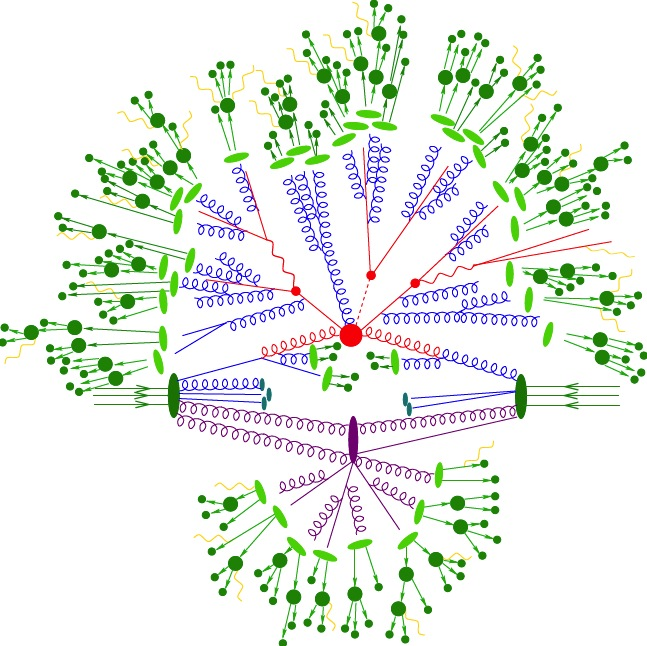
\includegraphics[width=\textwidth]{Figures/Generator_Event}
	\caption[An example simulation of a proton-proton collision showing all the various processes that must be modelled. Starting with the hard interaction in red calculated using perturbation theory, then dressing with additional soft processes in blue forming the parton shower. Additional parton interactions are added, shown in purple, each with a respective parton shower. Finally the parton shower is fragmented and hadronised into detectable, colourless hadrons, which can in turn decay and radiate. This fragmentation and hadronisation processes are shown in light green and green respectively. Photon radiation is shown in yellow. ]{An example simulation of a proton-proton collision showing all the various processes that must be modelled. Starting with the hard interaction in red calculated using perturbation theory, then dressing with additional soft processes in blue forming the parton shower. Additional parton interactions are added, shown in purple, each with a respective parton shower. Finally the parton shower is fragmented and hadronised into detectable, colourless hadrons, which can in turn decay and radiate. This fragmentation and hadronisation processes are shown in light green and green respectively. Photon radiation is shown in yellow.  Figure taken from~\cite{Gen:Event}.}
	\label{fig:GenEvent}
\end{figure}

\section{Hard interaction} % (fold)
\label{sec:hard_interaction}
The hard scattering process describes the interaction of two partons in the collider.
It is modelled through Eq~\ref{eq:pdf}, with the \acrshort{pdf}s taken from data convoluted with the partonic cross section.
The partonic cross section is calculated from the matrix-element of the interaction, directly taken from the Feynman diagrams through the Feynman rules.
If a short-lived resonance is formed as a result of the interaction, then its decay is also considered as part of the hard interaction.
Many matrix-elements can already be calculated to \acrshort{nnlo} or higher, however the generation of the hard scattering processes can currently only be calculated to \acrshort{lo} or \acrshort{nlo}.
This is simply due to the combinatorics when taking into account all possible Feynman diagrams.

There are a variety of matrix-element generators available, two of the most popular in high energy particle physics being \acrfull{mgamc}~\cite{Gen:MGamc} and \acrfull{powheg}~\cite{Gen:Pow1,Gen:Pow2,Gen:Pow3}.
The \acrshort{mgamc} matrix-element generator can model a process with additional partons.
The number of additional partons in the process depends on the complexity of the process, \eg{} for \acrshort{nlo} \ttbar{} production, an additional two partons can be generated.
It does this by adding real diagrams based on \acrshort{lo} or \acrshort{nlo} contributions from lower order processes.
In \acrshort{powheg}, virtual processes are included in the matrix element, up to one loop. 
This means that for \ttbar{} production, one less additional parton is able to be produced.
% Madgraph. Depending on the process a number of additional partons can be generated.
% at NLO
% e.g. tt at NLO: real contributions with respect to LO
% e.g. ttj at NLO: real NLO diagrams wrt tt at NLO
% e.g. ttjj at NLO: real NNLO diagrams wrt tt at NLO and real NLO diagrams wrt ttj at NLO
% at LO
% e.g. tt at LO: tree diagram
% e.g. ttj at LO: real NLO diagrams wrt tt at LO
% e.g. ttjj at LO: real NNLO diagrams wrt tt at LO and real NLO diagrams wrt ttj at LO
% e.g. ttjjj at LO: real NNNLO diagrams wrt ttjj at LO and real NNLO diagrams wrt ttj at LO and real NLO diagrams wrt ttj at LO


% section hard_interaction (end)

\section{Additional interactions and soft processes} % (fold)
\label{sec:additional_interactions_and_soft_processes}

Once the hard process has been simulated from the matrix-element calculations, additional hard, low-\pt{}, interactions need to be included. 
All the hard interactions then present in the simulation must be \textit{dressed} with soft emissions.

The most common hard process at the LHC is elastic gluon-gluon scattering, the cross section of which, diverges as the gluons become soft and collinear.
This means that below some momentum transfer threshold ($\sim5\GeV$) the inclusive jet production cross section from elastic gluon-gluon scattering is larger than the total inclusive proton-proton cross section~\cite{Gen:MPI_1,Gen:MPI_2}, which infers that for every collision, more than one interaction is occurring.
These are known as \textit{multiple parton interactions} (\acrshort{mpi}).
The number of additional interactions present is proportional to the impact parameter of the colliding protons.
A pair of protons colliding head on contains more additional interactions than a pair that collide obliquely.
% elastic = total here. dominated by t-channel processes

The extra soft emissions come in the form of \textit{initial} and \textit{final state radiation} (\acrshort{isr} and \acrshort{fsr}), where partons split from the hard interactions.
Figure~\ref{fig:feyn-ps} shows the four possible ways in which a parton can be radiated.
Firstly, a quark can radiate a gluon, secondly a gluon can pair-produce a \qqbar{} pair and finally there are two colour configurations of gluon splitting.
\begin{figure}[h!]
	\centering
	\begin{resizedtikzpicture}{0.45\linewidth}
		\begin{feynman}
			\vertex (A);
			\vertex [above=0.015cm of A] (aup);
			\vertex [below=0.015cm of A] (adown);

			\vertex [right=1.5cm of A] (B);
			\vertex [above=0.015cm of B] (bup);
			\vertex [below=0.015cm of B] (bdown);

			\vertex [above right=0.75cm and 1.5cm of B] (C);
			\vertex [above=0.015cm of C] (cup);
			\vertex [below=0.015cm of C] (cdown);
			\vertex [below right=0.75cm and 1.5cm of B] (D);
			\vertex [above=0.015cm of D] (dup);
			\vertex [below=0.015cm of D] (ddown);

			\diagram*{
			% (bup) -- [red,thick,edge label=\(\overline{r}\)] (dup),
			% (ddown) -- [electricgreen,thick,edge label=\(g\)] (bdown),
			% (B) -- [red,very thick,edge label=\(r\)] (C),
			% (A) -- [electricgreen,very thick,edge label=\(g\)] (B),
			(bup) -- [red,thick] (dup),
			(ddown) -- [electricgreen,thick] (bdown),
			(B) -- [red,very thick] (C),
			(A) -- [electricgreen,very thick] (B),
			(A) -- [fermion] (B),
			(B) -- [fermion] (C),
			(B) -- [gluon] (D),
			};
		\end{feynman}
		\end{resizedtikzpicture}
		\hspace{0.5cm}
		\begin{resizedtikzpicture}{0.45\linewidth}
		\begin{feynman}
			\vertex (A);
			\vertex [above=0.015cm of A] (aup);
			\vertex [below=0.015cm of A] (adown);

			\vertex [right=1.5cm of A] (B);
			\vertex [above=0.015cm of B] (bup);
			\vertex [below=0.015cm of B] (bdown);

			\vertex [above right=0.75cm and 1.5cm of B] (C);
			\vertex [above=0.015cm of C] (cup);
			\vertex [below=0.015cm of C] (cdown);
			\vertex [below right=0.75cm and 1.5cm of B] (D);
			\vertex [above=0.015cm of D] (dup);
			\vertex [below=0.015cm of D] (ddown);

			\diagram*{
			(aup) -- [red,thick] (bup),
			(adown) -- [electricgreen,thick] (bdown),
			(B) -- [red,very thick] (C),
			(B) -- [electricgreen,very thick] (D),

			(A) -- [gluon] (B),
			(B) -- [fermion] (C),
			(B) -- [anti fermion] (D),
			};
		\end{feynman}
		\end{resizedtikzpicture} \\
		\vspace{0.5cm}
		\begin{resizedtikzpicture}{0.45\linewidth}
		\begin{feynman}
			\vertex (A);
			\vertex [above=0.015cm of A] (aup);
			\vertex [below=0.015cm of A] (adown);

			\vertex [right=1.5cm of A] (B);
			\vertex [above=0.015cm of B] (bup);
			\vertex [below=0.015cm of B] (bdown);
			\vertex [right=0.025cm of B] (bright);
			\vertex [above=0.015cm of bright] (brightup);
			\vertex [below=0.015cm of bright] (brightdown);

			\vertex [above right=0.75cm and 1.5cm of B] (C);
			\vertex [above=0.015cm of C] (cup);
			\vertex [below=0.015cm of C] (cdown);
			\vertex [below right=0.75cm and 1.5cm of B] (D);
			\vertex [above=0.015cm of D] (dup);
			\vertex [below=0.015cm of D] (ddown);

			\diagram*{
			(bup) -- [red,thick] (cup),
			(bdown) -- [electricgreen,thick] (ddown),
			(bright) -- [blue,thick,sharp arrow angle=60,sharp right-] (cdown),
			(bright) -- [blue,thick,sharp arrow angle=60,sharp left-] (dup)
			(aup) -- [red,thick,sharp arrow angle=45,-sharp right] (brightup),
			(adown) -- [electricgreen,thick,sharp arrow angle=45,-sharp left] (brightdown),
			(A) -- [gluon] (B),
			(B) -- [gluon] (C),
			(B) -- [gluon] (D),
			};
		\end{feynman}
		\end{resizedtikzpicture}
		\hspace{0.5cm}
		\begin{resizedtikzpicture}{0.45\linewidth}
		\begin{feynman}
			\vertex (A);
			\vertex [above=0.015cm of A] (aup);
			\vertex [below=0.015cm of A] (adown);

			\vertex [right=1.5cm of A] (B);
			\vertex [above=0.015cm of B] (bup);
			\vertex [below=0.015cm of B] (bdown);
			\vertex [right=0.025cm of B] (bright);
			\vertex [above=0.015cm of bright] (brightup);
			\vertex [below=0.015cm of bright] (brightdown);

			\vertex [above right=0.75cm and 1.5cm of B] (C);
			\vertex [above=0.015cm of C] (cup);
			\vertex [below=0.015cm of C] (cdown);
			\vertex [below right=0.75cm and 1.5cm of B] (D);
			\vertex [above=0.015cm of D] (dup);
			\vertex [below=0.015cm of D] (ddown);

			\diagram*{
			(bright) -- [red,thick,sharp arrow angle=60,sharp left-] (dup),
			(bright) -- [electricgreen,thick,sharp arrow angle=60,sharp right-] (cdown),
			(bup) -- [blue,thick] (cup),
			(bdown) -- [blue,thick] (ddown),
			(aup) -- [red,thick,sharp arrow angle=45,-sharp right] (brightup),
			(adown) -- [electricgreen,thick,sharp arrow angle=45,-sharp left] (brightdown),
			(A) -- [gluon] (B),
			(B) -- [gluon] (C),
			(B) -- [gluon] (D),
			};
		\end{feynman}
		\end{resizedtikzpicture}
	\caption[The four possible processes to strongly split a parton in the parton shower. The top left panel shows gluon emission, the top right shows \qqbar{} pair production and the bottom two panels the colour configurations of gluon splitting. In addition, photon brehmsstrahlung from the quarks can occur but is not considered here.]{The four possible processes to strongly split a parton in the parton shower. The top left panel shows gluon emission, the top right shows \qqbar{} pair production and the bottom two panels the colour configurations of gluon splitting. In addition, photon brehmsstrahlung from the quarks can occur but is not considered here. }
	\label{fig:feyn-ps}
\end{figure}

For \acrshort{fsr}, the partons produced from the matrix-element calculation are split recursively until the energy of each remaining parton reduces to approximately 1\GeV{}, whereupon hadronisation effects become non-negligible.
In contrast, the \acrshort{isr} is modelled differently.
The longitudinal momentum fractions, $x_1$ and $x_2$, of the incoming partons are taken from the \acrshort{pdf} at the factorisation scale of the process and evolved backwards in time. 
The factorisation scale of an event is a cutoff where partons that carry a momentum less than the cutoff scale are absorbed into the \acrshort{pdf}.
If the momentum carried is above the scale then they participate in the interaction.
This ensures no divergences in the matrix-element due to collinear or soft gluons.
For every \acrshort{isr} emission, the parent parton must have the combined energy of the daughter parton and radiation.
There are however, fewer available partons carrying the increased fraction of the proton momentum, seen in the \acrshort{pdf} distribution, and so a suppression weight must be applied.
The suppression weight is derived from the \textit{Sudakov form factors}~\cite{Gen:Sudokov}.
In practice, the application of \acrshort{isr} and \acrshort{mpi} occur completely and in tandem, before the \acrshort{fsr} is modelled.

The collective spray of partons produced by the hard process, \acrshort{mpi}, \acrshort{isr} and \acrshort{fsr} is called the parton shower.
The evolution of the splittings in the parton shower is defined by ordering variables.
One such shower ordering variable is the square of the \pt{} of the shower propagators (\ktsq{}), such that \ktsq{} for a daughter splitting is less than the \ktsq{} for a mother splitting~\cite{Gen:kt}.
The splittings between \acrshort{mpi} can also be interleaved with one another.
The \ktsq{} ordering is illustrated in the left panel of Fig.~\ref{fig:feyn-ordering}, where the hard interaction occurs at $Q_{max}$ and the splitting strengths, given by $V_{i}(\ktsq{})$, are ordered $V_{1} > V_{2} > V_{3}$ (The further in time from the hard interaction, the softer and more collinear the splitting). 

Another way to evolve the shower is by using an angular ordering~\cite{Gen:angular}.
This angular ordering requires any future splitting to occur within a cone defined by the angular radius between the daughter partons from the previous splitting also illustrated in the right panel of Fig.~\ref{fig:feyn-ordering}.
These showers often produce wide-angle soft splittings before the main hard splitting.
% as would be the case in a \ktsq{}-ordered shower.
Two widely used models for the parton shower are \acrshort{pythia}~\cite{Gen:Pyth8p2} and \acrshort{herwig}~\cite{Gen:Herwigpp}, where \acrshort{pythia} uses a \ktsq{}-ordered shower and \acrshort{herwig} an angular-ordered shower.
\begin{figure}[h!]
\centering
\begin{resizedtikzpicture}{0.4\linewidth}
	\begin{feynman}
		\vertex (A);
		\vertex [right=1cm of A](C);
		\vertex [above=1.5cm of C](Ci);
		\vertex [below=0.05cm of C](C_quiet){\(V_{2}\)};
		\vertex [right=2.0cm of C](D);
		\vertex [above=0.05cm of D](D_quiet){\(Q_{max}\)};
		\vertex [right=2.5cm of D](F);
		\vertex [below=1.5cm of F](Fi);
		\vertex [left=0.05cm of Fi](F_quiet){\(V_{3}\)};
		\vertex [above right=0.75 cm and 1.5cm of Fi](Fii);
		\vertex [below right=0.75 cm and 1.5cm of Fi](Fiii);
		\vertex [right=1.5cm of F](G);

		\vertex [below=3cm of A](B);
		\vertex [right=3cm of B](E);
		\vertex [below=0.05cm of E](E_quiet){\(Q_{max}\)};
		\vertex [right=1.5cm of E](H);
		\vertex [above=0.05cm of H](H_quiet){\(V_{1}\)};
		\vertex [below=1.5cm of H](Hi);
		\vertex [right=2.5cm of H](I);

		\diagram* {
		(A) -- [fermion] (C),
		(C) -- [gluon] (Ci),
		(C) -- [fermion] (D),
		(D) -- [fermion] (F),
		(F) -- [gluon] (Fi),
		(Fi) -- [fermion] (Fii),
		(Fi) -- [anti fermion] (Fiii),
		(F) -- [fermion] (G),

		(B) -- [fermion] (E),
		(E) -- [fermion] (H),
		(H) -- [gluon] (Hi),
		(H) -- [fermion] (I),

		(D) -- [gluon] (E),
		};
	\end{feynman}
\end{resizedtikzpicture}
\hspace{0.4cm}
\begin{resizedtikzpicture}{0.56\linewidth}
	\begin{feynman}
		\vertex (A);
		\vertex [right=0.5cm of A](A_quiet){\(\theta_{max}\)};
		\vertex [left=1.5cm of A](Aminus);
		\vertex [below right=1.5cm and 1.5cm of A](A2);
		\vertex [above right=1.5cm and 1.5cm of A](B);
		\vertex [above right=0.2cm and 0.2cm of B](B_quiet){\(\theta_{1}\)};
		\vertex [above=1.5cm of B](C);
		\vertex [right=2.25cm of B](D);
		\vertex [right=0.5cm of D](D_quiet){\(\theta_{2}\)};
		\vertex [above right=1.25cm and 2.25cm of D](E);
		\vertex [above right=0.5cm and 1.25cm of E](E_quiet){\(\theta_{3}\)};
		\vertex [below right=1.25cm and 2.25cm of D](F);
		\vertex [below right=0.5cm and 1.25cm of F](F_quiet){\(\theta_{4}\)};
		\vertex [above right=1.5cm and 1.75cm of E](G);
		\vertex [above right=0.5cm and 2.25cm of E](H);
		\vertex [below right=1.5cm and 1.75cm of F](I);
		\vertex [below right=0.5cm and 2.25cm of F](J);

		\diagram* {
		(Aminus) -- [gluon] (A),
		(A) -- [anti fermion] (A2),
		(A) -- [fermion] (B),
		(B) -- [gluon] (C),
		(B) -- [fermion] (D),
		(D) -- [gluon] (E),
		(D) -- [fermion] (F),
		(E) -- [fermion] (G),
		(E) -- [anti fermion] (H),
		(F) -- [fermion] (I),
		(F) -- [gluon] (J),
		};
	\end{feynman}
\end{resizedtikzpicture}
\caption[The left panel shows parton shower ordering by \ktsq{} where the splitting strength $V_{i}(\ktsq)$ is ordered $V_1 > V_2 > V_3$. The right panel shows shower ordering by angle such that the opening angle decreases for every consecutive splitting $\theta_{max} > \theta_{1} > \theta_{2} > \theta_{3, 4}$.]{The left panel shows parton shower ordering by \ktsq{} where the splitting strength $V_{i}(\ktsq)$ is ordered $V_1 > V_2 > V_3$. The right panel shows shower ordering by angle such that the opening angle decreases for every consecutive splitting $\theta_{max} > \theta_{1} > \theta_{2} > \theta_{3, 4}$.}
\label{fig:feyn-ordering}
\end{figure}


% http://citeseerx.ist.psu.edu/viewdoc/download?doi=10.1.1.575.1213&rep=rep1&type=pdf
% http://www.hep.phy.cam.ac.uk/seminars/talks/2008/michaelmas/PaoloNason-14102008.pdf
% https://indico.cern.ch/event/35476/contributions/1760582/attachments/703609/965976/krauss_showers.pdf
% http://cds.cern.ch/record/694095/files/0312274.pdf
% http://www.iaea.org/inis/collection/NCLCollectionStore/_Public/45/031/45031526.pdf
% https://arxiv.org/pdf/1411.4085.pdf
% section additional_interactions_and_soft_processes (end)


\section{Matching matrix-elements to parton showers} % (fold)
\label{sec:matching_matrix_elements_to_parton_showers}

Parton showers and higher-order matrix-element calculations describe the same physics and so need to be combined consistently.
The soft emissions added from the parton shower should interface with the matrix-element based radiation with no gaps or overlaps for a specific, fixed final state parton multiplicity.
This problem is solved by a process known as \textit{matching}.
% TODO MERGING?

One method of matching, known as the \acrshort{mlm}-method~\cite{Gen:MLM}, after its author M. L. Mangano, matches the final state partons produced by the matrix-element calculation to parton jets created by clustering the showered partons.
The angular distance from each final state parton to each parton jet, starting from the parton with the leading \pt{}, is calculated and is said to be matched if it is less than a threshold value.
If the matching is successful the parton jet is removed from further calculations.
All final state partons must be matched to parton jets, otherwise the event is rejected.
When simulating the hard interaction process, including contributions with up to $N$ additional partons, events in samples simulated with $n$ additional partons, where $n<N$, are suppressed if they do not contain exactly $n$ matched parton jets.
This is because these events are present and more accurately modelled in the $n+1$ production sample and thus double counting is avoided.
All the production samples generated using discrete additional parton multiplicities are subsequently \textit{merged}.

When matching and merging at \acrshort{nlo} the additional parton jet from the matrix-element calculation is the hardest emission and thus defines the upper shower scale level.
While it is easy to interface this with showers ordered to some \pt{}, care must be taken with respect to an angular-ordered shower.
Angular-ordered shower emissions with a \pt{} greater than the additional matrix-element parton jet need to be suppressed.
The \FxFx{}-method~\cite{Gen:FXFX}, extends the \acrshort{mlm}-method of merging to matrix-elements calculated to \acrshort{nlo}.
The \acrshort{mlm}-method is used when matching \acrshort{lo} \acrshort{mgamc} to \acrshort{pythia} and the \FxFx{}-method is used when matching \acrshort{nlo} \acrshort{mgamc} to \acrshort{pythia}.

When \acrshort{powheg} models processes at a large factorisation scale, the number of high-\pt{} soft emissions is overestimated. 
It is resolved by introducing a \pt{} dependent damping factor, 
\begin{equation*}
	D = \frac{\hdamp^2}{\pt^2+\hdamp^2},
\end{equation*}
where \hdamp{} is the damping parameter, usually set to the factorisation scale (in the case for top quark production to $m_t$).
$D$ effectively sets the upper-\pt{} limit for the first additional emission and hence the upper shower scale level.

% Either start with higher Q2 in parton and evolve forwards. 
% Inefficient as prob here of this is small. 
% Or start with lower Q2 and evolve backwards.
% Matching - procedure to obtain a smooth transition for a fixed parton multiplicity
% Merging - the combination of several multiplicities
% Discarded e.g. if two partons match to the same jet (merged) or if parton not energetic enough to produce a jet.

% section matching_matrix_elements_to_parton_showers (end)

\section{Fragmentation and colour reconnection} % (fold)
\label{sec:fragmentation_and_colour_reconnection}

The fragmentation process models how final state partons from the parton shower hadronise into colourless states.
There are two general methods in use for the fragmentation, the \textit{Lund string model}~\cite{Gen:LundString1,Gen:Pyth8p2} and the \textit{cluster model}~\cite{Gen:Herwigpp}.

\subsection{Lund string model} % (fold)
\label{sub:string_fragmentation}

Due to the self interactions of gluons, the strong field between two quarks can be represented by a confined tube of dimension $1+1$, otherwise known as a string. 
As the quarks move apart the potential energy in the string increases linearly by 1\GeV{}\fminv{}.
At some point the colour field contains enough potential energy that it is favourable to pair-produce light quarks, which combine with the initial quarks to form two new colourless particles, breaking the string.
The string is stretched between quark endpoints by a number of gluons.
Each gluon results in a kink to the string that depends on the kinematic properties of the gluon.
The left panel of Fig.~\ref{fig:Lund} shows the kink in a string produced by the addition of a gluon and the right panel shows the fragmentation of the string.
\begin{figure}[htpb]
	\centering
	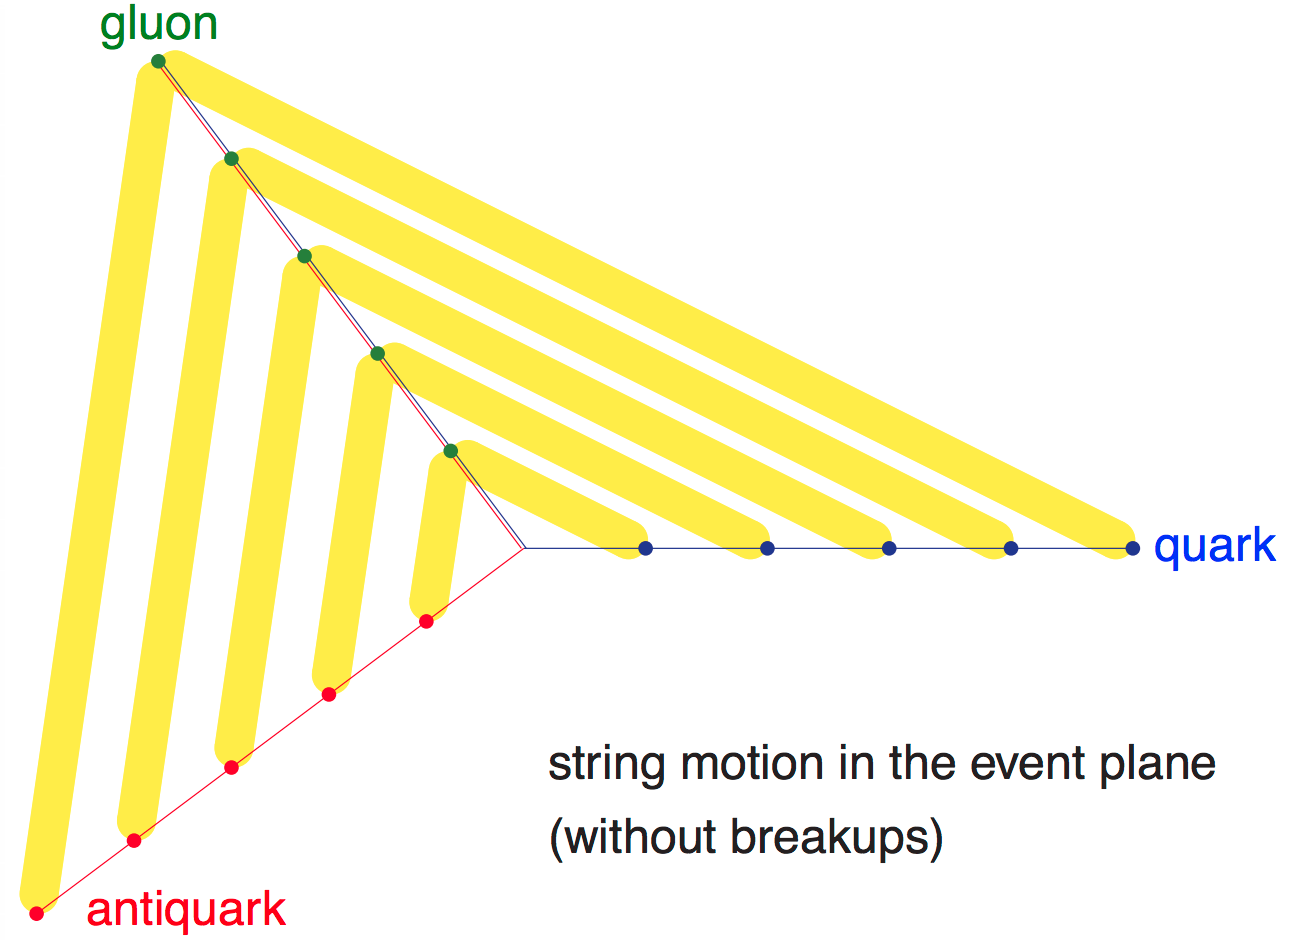
\includegraphics[width=0.43\textwidth]{Figures/Generator_Lund2}
	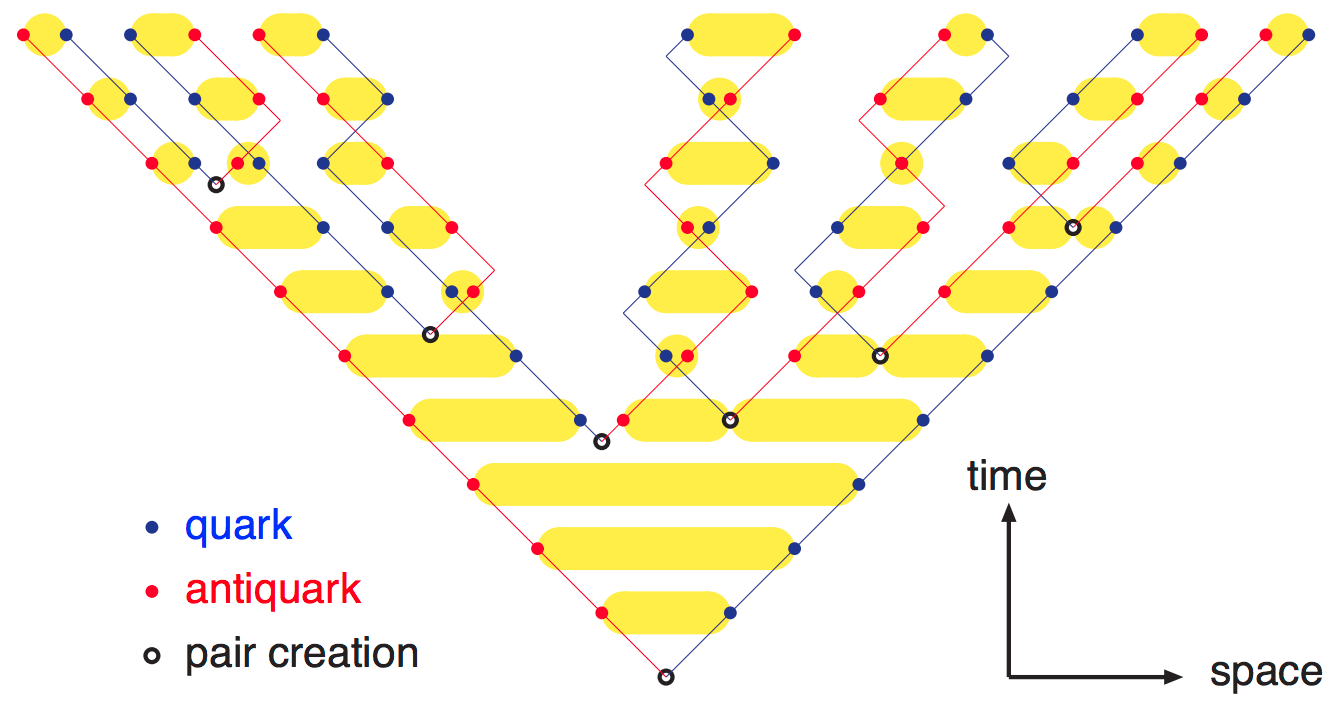
\includegraphics[width=0.56\textwidth]{Figures/Generator_Lund}
	\caption[The left panel shows the string between the quark-antiquark colour dipole stretched by a gluon and the right panel shows for each string how fragmentation occurs with time. Lorentz boosts in the hadrons are shown by oscillation frequency. ]{The left panel shows the string between the quark-antiquark colour dipole stretched by a gluon and the right panel shows for each string how fragmentation occurs with time. Lorentz boosts in the hadrons are shown by oscillation frequency. Figures taken from~\cite{Gen:Lund}.}
	\label{fig:Lund}
\end{figure}
As time evolves, if \qqbar{} pairs do not have enough potential in the colour field to pair-produce they end up bound to each other forming the colourless mesons of the final state.
It is also possible for the potential in the colour field to be great enough to produce diquark-diantiquark pair instead of \qqbar{} with the end result being the formation of baryons instead of mesons.
This approach is used in the \acrshort{pythia} parton shower simulation.
% pg10 https://indico.cern.ch/event/564031/contributions/2279204/attachments/1326142/1990851/16-FNAL-pp.pdf

The string dynamics currently assume that the colour-flow modelled in the evolution of the parton shower from the hard interaction is independent from the colour-flow of the other parton showers produced by the \acrshort{mpi}s.
Indeed, each individual \acrshort{mpi} is assumed to operate in independent colour spaces.
In reality, all the individual interactions are superimposed on each other, with soft gluons connecting all the final state partons from all sources, redistributing colour across the full parton shower.
In the Lund string model this can have the effect of reorganising the strings produced in the parton shower.
This is modelled in simulation by a process known as \textit{colour reconnection} (\acrshort{cr}), which reconfigures the colour strings after the parton shower, but before the fragmentation.
Three different models which can be implemented using \acrshort{pythia} are described here.
% MPIs happen between protons radius == transverse size of the qcd string == non independent simulation

\subsubsection{MPI-based model} % (fold)
\label{sub:mpi_based_model}

The \textit{MPI-based} \acrshort{cr} model~\cite{Gen:GluonMove} calculates the reconnection probability for all gluons from lower-\pt{} interactions to be inserted into the colour-flow dipoles of a higher-\pt{} interaction.
Once all reconnections between \acrshort{mpi}s have been identified, the configuration in which the total colour string length is minimised is selected.
The \acrshort{pythia} parton shower simulation uses the \acrshort{mpi}-based \acrshort{cr} scheme as default, where it is assumed that the lifetime of the top quark is long enough to shield the top decay products from the effects of \acrshort{cr}.
A second \acrshort{mpi}-based model exists where the top quark decays before the \acrshort{cr} is applied and as such the top decay products are able to reconnect.
This is known as \acrshort{mpi}-based \acrshort{cr} with \textit{early resonance decays} (erdON).
% Prob is higher for lower pt MPIs due to increased wavefunctions, which leads to higher spread and chance to interfere.
% Starting at ordered high-pt, look at colour reconnections to lower MPIs. Gluons are inserted between MPIs in such a way to minimize string length.

% The \acrshort{mpi}-based \acrshort{cr} model takes \acrshort{mpi}s, iterating in order of increasing hardness, and calculates a reconnection probability to \acrshort{mpi} with the next highest \pt{}.
% If no reconnection is found, consecutively harder \acrshort{mpi}s are tested.
% ERD: The \textit{gluon move/flip} model \cite{Gen:GluonMove} of the \acrshort{cr} starts from the default \acrshort{mpi}-based model. 
% The top quarks then decay and radiate, from which a second set of \acrshort{cr} occurs between radiated gluons from the top decay and those from the rest of the parton shower.
% subsubsection mpi_based_model (end)

\subsubsection{QCD-inspired model} % (fold)
\label{sub:qcd_inspired_model}

An alternative \acrshort{cr} model is the \textit{QCD-inspired} model~\cite{Gen:QCDBased}.
In this model, instead of the $\mathrm{SU(3)}$ colour indices ($r,g,b$) being applied to individual partons, a set of nine indices, which describe the possible colour states of 2-parton and 3-parton combinations, are used.
A corresponding set of anti-colour indices is used for anti-quarks and a gluon contains one of each index.
Reconnections are possible when two partons have a matching colour and anti-colour index.
The set of possible reconnections encompasses every possible reconnection from the default \MPI-based \acrshort{cr} model as well as reconnections possible between partons with accidentally matching colour indices.
As with the \MPI-based \acrshort{cr} model, a reconnection is performed if it minimises the total \acrshort{qcd} string length.
% subsubsection qcd_inspired_model (end)

\subsubsection{Gluon move/flip model} % (fold)
\label{sub:gluon_move_flip_model}

The \textit{gluon move/flip} model~\cite{Gen:GluonMove}, moves all final state gluons between colour strings so that the total string length is minimised. 
However, by moving only gluons, no quarks are able to reconnect and so a subsequent procedure is applied in which two colour segments are flipped between colour strings.
As with moving the gluons, the solution which minimises the total string length is used.
% a subset of final state gluons can be used given by a colour reconnection strength parameter.
% subsubsection gluon_move_flip_model (end)
% subsection string_fragmentation (end)
% section colour_reconnection (end)


\subsection{Cluster fragmentation model} % (fold)
\label{sub:cluster_fragmentation}

In the cluster model of fragmentation implemented in the \acrshort{herwig} parton shower simulation, all partons are showered until they reach an energy scale of $\sim4\GeV$, where hadronisation effects become non-negligible.
The final state gluons must have an energy at least twice that of the invariant mass of the lightest quark and are forced to split into a \qqbar{} pair.
The colour singlet states formed by the resulting colour connected partons are formed into clusters, as shown in Fig.~\ref{fig:Cluster}.
The cluster model assumes the principle of \textit{colour-preconfinement} which states that the distribution of the mass of the clusters is independent of the centre-of-mass energy and the hard scattering process involved.
Most clusters are distributed at low masses and can be regarded as excited hadron resonances and decayed into observed hadrons, however some clusters are too massive for this to be realistic and split in a process called \textit{cluster fission}.
If fission is required, a \qqbar{} pair of \uquark{}, \dquark{} or \squark{} flavour, is taken from the vacuum and the cluster split such that one of the original quarks is contained in each new cluster.
Fissions continue until all clusters are accepted by the mass parameters of the model.
The final process of the fragmentation involves extracting a \qqbar{} or \qqqbarqbar{} from vacuum in each cluster, forming a pair of hadrons, which in turn may decay into lighter hadrons.

\begin{figure}[htpb]
	\centering
	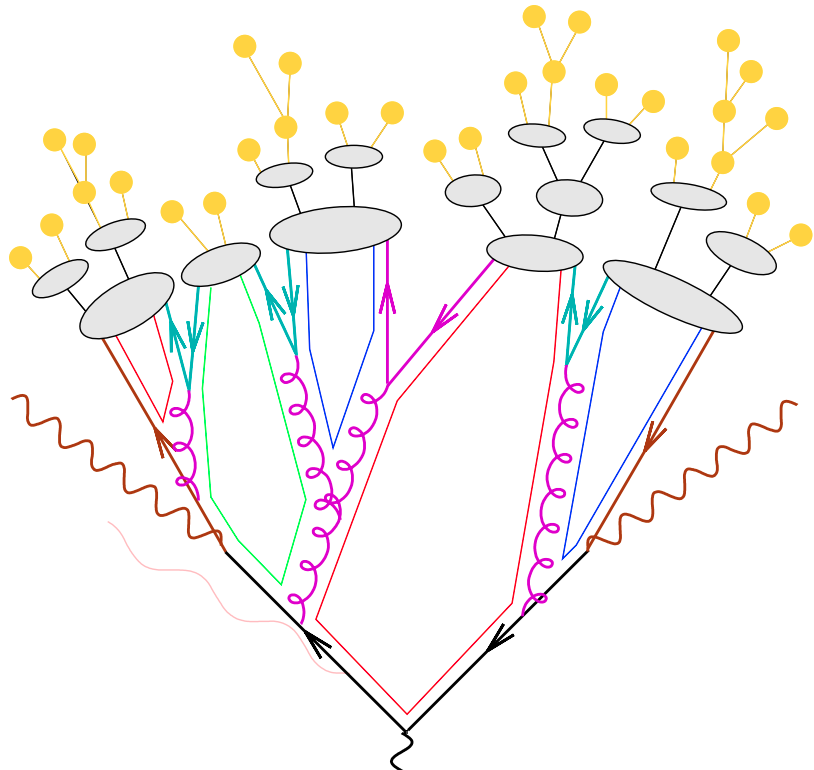
\includegraphics[width=0.6\textwidth]{Figures/Generator_Cluster}
	\caption[A sketch of the cluster model of fragmentation and hadronisation. Colour singlet clusters are generated from the final state quarks and gluons forced to split into a \qqbar{} pair. These colour singlet clusters can be unnaturally massive and fission occurs until the clusters represent excited hadron resonances which then hadronise. ]{A sketch of the cluster model of fragmentation and hadronisation. Colour singlet clusters are generated from the final state quarks and gluons forced to split into a \qqbar{} pair. These colour singlet clusters can be unnaturally massive and fission occurs until the clusters represent excited hadron resonances which then hadronise.  Figure adapted from \cite{Gen:Cluster}.}
	\label{fig:Cluster}
\end{figure}
% For cluster model, to conserve colour - intial partons must come from valence. gluon -> valence and emits anti quark. seaquark -> gluon -> valence. remnent qq collur triplet, valence: colour triplet
% gluon splitting to diquark pair not suported
% M^Clpow ≥ Clmax^Clpow + (m1 + m2)^Clpow. Clmax: max cluster mass. Clpow: mass exponent. m1,2 mass of cluster quark compentents
% the masses of the daughter clusters are required to be less than that of the parent cluster and greater than the sum of the masses of their constituent partons.
% flavour mixing in light hadrons.
% all probabilities depend on phase space. complicated and covered by model parameters

% subsection cluster_fragmentation (end)



% \begin{equation}
% 	\frac{dP}{d\pt} \propto \kappa (e^{\frac{\pi m_{\mathrm{T}}^2}{\kappa}})
% \end{equation}
% Dont know where this is from ^
% section fragmentation_and_colour_reconnection (end)





\section{Detector modelling} % (fold)
\label{sec:detector_modelling}

So far, only the modelling of the physics process itself has been discussed, before any interaction with the detector has been performed.
Indeed, it is very useful to compare measurements at this level, the \textit{particle level}, as it allows direct comparisons between theoretical models and experimental measurements which have had the detector response removed.
The removal of the detector response is discussed in Ch.~\ref{ch:unfolding}.
This means measurements performed to particle level with different detectors such as \acrshort{cms} and \acrshort{atlas} can be directly compared with each other and to theoretical predictions.

In order to provide the mapping between experiment and particle level, the detector response needs to be modelled accurately.
To do this a simulation toolkit called \textit{GEometry ANd Tracking} (\acrshort{geant})~\cite{Gen:GEANT} is used.
The \acrshort{geant} package builds the physical layout of the experiment, including all detectors, absorbers, electronics and structural components surrounding the central interaction point.
The magnetic field strength at all points in the detector is modelled.
The particles are tracked from the collision point outwards through the active and non-active material, modelling respective interactions and decays.
In the active material, the response of all individual components is modelled in a process known as \textit{digitisation}.
The digitisation takes into account any inefficiencies in the active material and returns an output consistent with that seen from measured data.
A full description of the \acrshort{cms} detector is given in Ch.~\ref{ch:LHCCMS}.

% Not quite -phase space issues.
% section detector_modelling (end)

\section{Production of $\mathbf{t\overline{t}}$ and background models}
\label{sec:ttMC}

Table~\ref{tb:Gen} shows the complete set of simulations used for the differential cross section analysis performed.
There are four different \ttbar{} production models studied.
Two \ttbar{} samples are simulated with the \acrshort{powheg} (v2) matrix element generator~\cite{Gen:PowHVF}, where one sample is interfaced with \acrshort{pythia} (v8.212), using the \CUET{} tune~\cite{Gen:CUETP8M2T4}, and the second with the \acrshort{herwig} (v2.7.1) using the \herwigtune{} tune~\cite{Gen:EE5C}.
These are labelled \powhegpythia{} and \powhegherwig{} respectively.
Two additional simulated \ttbar samples are produced with the \acrshort{mgamc} (v2.2.2) generator.
One is used to generate events at \acrshort{lo} accuracy with up to three additional partons and the second to \acrshort{nlo} accuracy with up to two additional partons.
Both are interfaced with \acrshort{pythia} using the \CUETold{} tune~\cite{Gen:CUETP8M1} and are labelled \mgamcLO{} and \mgamcNLO{} respectively.
The \acrshort{mlm} jet-parton matching algorithm is used to match the matrix-element to the parton shower in the \acrshort{lo} simulation and the \FxFx{} algorithm in the \acrshort{nlo} simulation.
The \powhegpythia{} model is taken as the central model used in this thesis.

All \ttbar{} production samples are simulated with the top quark mass set to 172.5\GeV{}.
For \acrshort{nlo} samples the \nnpdf{} \acrshort{pdf} set~\cite{Gen:NNPDF} is used, while for \acrshort{lo} samples the \nnpdflo{} set is used.
The samples are normalised to a \acrshort{nnlo} \ttbar{} cross section of 832\pb{}, as seen in Sec.~\ref{sub:top_quark_production}.
It is important to compare multiple \ttbar{} generators in order to find the current most suitable description of top quark production and decay, and to identify any discrepancies in the models.

Table~\ref{tb:Gen} also shows the dominant background samples from single top quark production, vector boson production with associated jets and multi-jet \acrshort{qcd} production.
All the single top quark processes produced via the $t$-channel and in association with a \Wboson{}~boson are generated with \acrshort{powheg}~\cite{Gen:Pow_tchan,Gen:Pow_tWchan} interfaced with \acrshort{pythia} and are normalised to cross sections that are calculated to \acrshort{nlo} precision~\cite{Gen:ST_XSECPred_1,Gen:ST_XSECPred_2}.  
Samples of \Wboson{}{} and \Zboson{}~boson production in association with jets, with leptonic final states, are generated at \acrshort{lo} using \acrshort{mgamc}. 
Separate samples are generated with exactly one, two, three, and four additional jets to ensure a large set of background events.
These samples are normalized to their \acrshort{nnlo} cross sections~\cite{Gen:VJets_XSECPred}.
Multijet \acrshort{qcd} events are generated using \acrshort{pythia} for both the matrix-element calculations and parton shower/hadronisation.
Only multijet \acrshort{qcd} events with large electromagnetic activity or that contain a muon are generated in order to maximise the available sample size.

The simulated samples need to contain enough events to ensure they are not affected by statistical fluctuations when comparing to the data.
The luminosity, described in further detail in Sec.~\ref{sec:lumi}, produced for each simulation sample is shown in the final column of Tab.~\ref{tb:Gen} and should ideally be comparable to or larger than the luminosity of the data collected.
Looking ahead to Tab.~\ref{tb:Data2016}, the total collected data luminosity is 35.9\fbinv{} and so most of the signal and background samples do indeed contain enough events.
The multijet \acrshort{qcd} events are not particularly well modelled and can suffer from a lack of statistics and so a data-driven multijet \acrshort{qcd} estimate is employed, which is described in Sec.~\ref{sec:multijet_qcd}.
The multijet \acrshort{qcd} samples are still required in the creation of the estimate however.

Samples are also generated for variations of some of the generator parameters in \powhegpythia{}.
These are shown in Tab.~\ref{tb:GenSys} and are used as part of the estimation of the theoretical uncertainties due to the modelling.
Other theoretical uncertainties in the modelling are calculated as event weights and stored in the central \powhegpythia{} sample.
The CMS detector response for all simulated samples is modelled using \acrshort{geant}.

\begin{table}
	\centering
		\caption{The set of simulated samples used in this thesis. They include four different signal \ttbar{} production samples and samples for the background production. The backgrounds are single top quark production, vector boson production in association with jets and multijet \QCD{}. }
		\label{tb:Gen}
		\resizebox{\linewidth}{!}{%
		\begin{tabular}{llllccc}
			 	& \textbf{Matrix}	& \textbf{Parton} & \textbf{Tune}	& \textbf{Cross section} 	  			& \textbf{Events}  	& \textbf{Luminosity} 	\\
			 	& \textbf{element}	& \textbf{shower} &  				& \textbf{(\pb{})} 	&  	\textbf{(\ten{6})}	& \textbf{(\fbinv{})} 	\\
			\multicolumn{7}{l}{\textbf{Models of \ttbar{} production}} \\
			\hline
			\vspace*{0.02cm}
			\powhegpythia{} & \powheg{} & \pythia{} & \CUET{}		& 831.76 & 154.9 & 186.3 \\ 
			\powhegherwig{} & \powheg{} & \herwig{} & \herwigtune{}	& 831.76 & 59.2  & 77.1 \\ 
			\mgamcLO{} 		& \mgamc{}	& \pythia{} & \CUETold{}  	& 831.76 & 10.1  & 12.2 \\ 
			\mgamcNLO{} 	& \mgamc{}	& \pythia{} & \CUETold{}  	& 831.76 & 30.4  & 36.6 \\ 

			\vspace*{0.02cm} \\
			\multicolumn{7}{l}{\textbf{Models of single top background production}} \\
			\hline
			\vspace*{0.02cm}
			Single top $t$-channel 			& \powheg{} 			& \pythia{} &	\CUETold{}  & 136.02	  & 66.9  & 492.0 \\ 
			Single anti-top $t$-channel	 	& \powheg{} 			& \pythia{} &	\CUETold{}  & 80.95	  	  & 38.8  & 479.4 \\ 
			Single top $tW$-channel 		& \powheg{} (v1)		& \pythia{} &	\CUETold{}  & 35.6		  & 7.9   & 223.2 \\ 
			Single anti-top $tW$-channel 	& \powheg{} (v1)		& \pythia{} &	\CUETold{}  & 35.6		  & 7.9   & 222.8 \\ 
			Single top/anti-top $s$-channel & \mgamc{} 				& \pythia{} &	\CUETold{}  & 6.35		  & 0.6    & 98.1 \\ 

			\vspace*{0.02cm} \\
			\multicolumn{7}{l}{\textbf{Models of vector boson background production}} \\
			\hline 
			\vspace*{0.01cm}
			Drell-Yan + 1 jet 			& \mgamc{}			& \pythia{} &	\CUETold{}	 & 	1016		  &  62.6  & 61.6 \\ 
			Drell-Yan + 2 jets  		& \mgamc{}			& \pythia{} &	\CUETold{}	 & 	331.4		  &  20.0  & 60.3 \\ 
			Drell-Yan + 3 jets  		& \mgamc{}			& \pythia{} &	\CUETold{}	 & 	96.36		  &  5.9   & 60.8 \\ 
			Drell-Yan + 4 jets  		& \mgamc{}			& \pythia{} &	\CUETold{}	 & 	51.4		  &  4.2   & 81.7 \\ 
			\Wboson{} boson + 1 jet 	& \mgamc{}			& \pythia{} &	\CUETold{}	 & 	9493		  &  45.4  & 4.8 \\ 
			\Wboson{} boson + 2 jets 	& \mgamc{}			& \pythia{} &	\CUETold{}	 & 	3120		  &  60.2  & 19.3 \\ 
			\Wboson{} boson + 3 jets 	& \mgamc{}			& \pythia{} &	\CUETold{}	 & 	942.3		  &  59.1  & 62.7 \\ 
			\Wboson{} boson + 4 jets 	& \mgamc{}			& \pythia{} &	\CUETold{}	 & 	524.2		  &  30.0  & 57.2 \\ 

			\vspace*{0.02cm} \\
			\multicolumn{7}{l}{\textbf{Models of multijet \QCD{} background production}} \\
			\hline 
			\vspace*{0.02cm}
			Muon enriched \QCD (20-30) 			& \pythia{}			& \pythia{} &	\CUETold{}	 & 	558528000 * 0.0053		  &  30.6  & 0.01 \\ 
			Muon enriched \QCD (30-50) 			& \pythia{}			& \pythia{} &	\CUETold{}	 & 	139803000 * 0.01182		  &  30.0  & 0.02 \\ 
			Muon enriched \QCD (50-80) 			& \pythia{}			& \pythia{} &	\CUETold{}	 & 	19222500 * 0.02276		  &  19.8  & 0.04 \\ 
			Muon enriched \QCD (80-120) 		& \pythia{}			& \pythia{} &	\CUETold{}	 & 	2758420 * 0.03844		  &  23.6  & 0.2 \\ 
			Muon enriched \QCD (120-170) 		& \pythia{}			& \pythia{} &	\CUETold{}	 & 	469797 * 0.05362		  &  8.0  & 0.3 \\ 
			Muon enriched \QCD (170-300) 		& \pythia{}			& \pythia{} &	\CUETold{}	 & 	117989 * 0.07335		  &  17.4  & 2.0 \\ 
			Muon enriched \QCD (300-470) 		& \pythia{}			& \pythia{} &	\CUETold{}	 & 	7820.25 * 0.10196		  &  49.0  & 61.4 \\ 
			Muon enriched \QCD (470-600) 		& \pythia{}			& \pythia{} &	\CUETold{}	 & 	645.528 * 0.12242		  &  19.0  & 240.1 \\ 
			Muon enriched \QCD (600-800) 		& \pythia{}			& \pythia{} &	\CUETold{}	 & 	187.109 * 0.13412		  &  10.0  & 397.7 \\ 
			Muon enriched \QCD (800-1000) 		& \pythia{}			& \pythia{} &	\CUETold{}	 & 	32.3486 * 0.14552		  &  19.8  & 4199.3 \\ 
			Muon enriched \QCD (1000-Inf) 		& \pythia{}			& \pythia{} &	\CUETold{}	 & 	10.4305 * 0.15544		  &  13.4  & 8264.9 \\

			Electron enriched \QCD (20-30) 		& \pythia{}			& \pythia{} &	\CUETold{}	 & 557600000 * 0.0096		  & 9.2  & 0.002 \\ 
			Electron enriched \QCD (30-50) 		& \pythia{}			& \pythia{} &	\CUETold{}	 & 136000000 * 0.073		  & 6.8  & 0.0007 \\ 
			Electron enriched \QCD (50-80) 		& \pythia{}			& \pythia{} &	\CUETold{}	 & 19800000 * 0.146			  & 45.2  & 0.02 \\ 
			Electron enriched \QCD (80-120) 	& \pythia{}			& \pythia{} &	\CUETold{}	 & 2800000 * 0.125			  & 76.5  & 0.2 \\ 
			Electron enriched \QCD (120-170) 	& \pythia{}			& \pythia{} &	\CUETold{}	 & 477000 * 0.132			  & 77.8  & 1.2 \\ 
			Electron enriched \QCD (170-300) 	& \pythia{}			& \pythia{} &	\CUETold{}	 & 114000 * 0.165			  & 11.5  & 0.6 \\ 
			Electron enriched \QCD (300-Inf) 	& \pythia{}			& \pythia{} &	\CUETold{}	 & 9000 * 0.15			 	  & 7.4  & 54.6 \\ 
			
			bc to E \QCD (30-80) 				& \pythia{}			& \pythia{} &	\CUETold{}	 & 	159068000 * 0.00255 & 15.3   & 0.04 \\ 
			bc to E \QCD (80-170) 				& \pythia{}			& \pythia{} &	\CUETold{}	 & 	3221000 * 0.01183  	& 14.9   & 0.4 \\ 
			bc to E \QCD (170-250) 				& \pythia{}			& \pythia{} &	\CUETold{}	 & 	105771 * 0.02492  	& 9.7   & 3.9 \\ 
			bc to E \QCD (250-Inf) 				& \pythia{}			& \pythia{} &	\CUETold{}	 & 	21094.1 * 0.03375 	& 9.8   & 13.7 \\ 
		\end{tabular}%
	}
\end{table}

			% \powhegpythia{} & \powheg{} & \pythia{} & \CUET{}		& 831.76 & 154948894 & 186.3 \\ 
			% \powhegherwig{} & \powheg{} & \herwig{} & \herwigtune{}	& 831.76 & 59174465  & 77.1 \\ 
			% \mgamcLO{} 		& \mgamc{}	& \pythia{} & \CUETold{}  	& 831.76 & 10139950  & 12.2 \\ 
			% \mgamcNLO{} 	& \mgamc{}	& \pythia{} & \CUETold{}  	& 831.76 & 30414083  & 36.6 \\ 
			% Single top $t$-channel 			& \powheg{} 			& \pythia{} &	\CUETold{}  & 136.02	  & 66928232  & 492.0 \\ 
			% Single anti-top $t$-channel	 	& \powheg{} 			& \pythia{} &	\CUETold{}  & 80.95	  	  & 38811017  & 479.4 \\ 
			% Single top $tW$-channel 		& \powheg{} (v1)		& \pythia{} &	\CUETold{}  & 35.6		  & 7944854   & 223.2 \\ 
			% Single anti-top $tW$-channel 	& \powheg{} (v1)		& \pythia{} &	\CUETold{}  & 35.6		  & 7931370   & 222.8 \\ 
			% Single top/anti-top $s$-channel & \mgamc{} 				& \pythia{} &	\CUETold{}  & 6.35		  & 622990    & 98.1 \\ 
			% Drell-Yan + 1 jet 			& \mgamc{}			& \pythia{} &	\CUETold{}	 & 	1016		  &  62627174  & 61.6 \\ 
			% Drell-Yan + 2 jets  		& \mgamc{}			& \pythia{} &	\CUETold{}	 & 	331.4		  &  19970551  & 60.3 \\ 
			% Drell-Yan + 3 jets  		& \mgamc{}			& \pythia{} &	\CUETold{}	 & 	96.36		  &  5856110   & 60.8 \\ 
			% Drell-Yan + 4 jets  		& \mgamc{}			& \pythia{} &	\CUETold{}	 & 	51.4		  &  4197868   & 81.7 \\ 
			% \Wboson{} boson + 1 jet 	& \mgamc{}			& \pythia{} &	\CUETold{}	 & 	9493		  &  45367044  & 4.8 \\ 
			% \Wboson{} boson + 2 jets 	& \mgamc{}			& \pythia{} &	\CUETold{}	 & 	3120		  &  60197766  & 19.3 \\ 
			% \Wboson{} boson + 3 jets 	& \mgamc{}			& \pythia{} &	\CUETold{}	 & 	942.3		  &  59067548  & 62.7 \\ 
			% \Wboson{} boson + 4 jets 	& \mgamc{}			& \pythia{} &	\CUETold{}	 & 	524.2		  &  29995313  & 57.2 \\ 
			% Muon enriched \QCD (20-30) 			& \pythia{}			& \pythia{} &	\CUETold{}	 & 	558528000 * 0.0053		  &  30613738  & 0.01 \\ 
			% Muon enriched \QCD (30-50) 			& \pythia{}			& \pythia{} &	\CUETold{}	 & 	139803000 * 0.01182		  &  29954815  & 0.02 \\ 
			% Muon enriched \QCD (50-80) 			& \pythia{}			& \pythia{} &	\CUETold{}	 & 	19222500 * 0.02276		  &  19806915  & 0.04 \\ 
			% Muon enriched \QCD (80-120) 		& \pythia{}			& \pythia{} &	\CUETold{}	 & 	2758420 * 0.03844		  &  23584215  & 0.2 \\ 
			% Muon enriched \QCD (120-170) 		& \pythia{}			& \pythia{} &	\CUETold{}	 & 	469797 * 0.05362		  &  8042721  & 0.3 \\ 
			% Muon enriched \QCD (170-300) 		& \pythia{}			& \pythia{} &	\CUETold{}	 & 	117989 * 0.07335		  &  17350231  & 2.0 \\ 
			% Muon enriched \QCD (300-470) 		& \pythia{}			& \pythia{} &	\CUETold{}	 & 	7820.25 * 0.10196		  &  48995686  & 61.4 \\ 
			% Muon enriched \QCD (470-600) 		& \pythia{}			& \pythia{} &	\CUETold{}	 & 	645.528 * 0.12242		  &  18976018  & 240.1 \\ 
			% Muon enriched \QCD (600-800) 		& \pythia{}			& \pythia{} &	\CUETold{}	 & 	187.109 * 0.13412		  &  9981311  & 397.7 \\ 
			% Muon enriched \QCD (800-1000) 		& \pythia{}			& \pythia{} &	\CUETold{}	 & 	32.3486 * 0.14552		  &  19767439  & 4199.3 \\ 
			% Muon enriched \QCD (1000-Inf) 		& \pythia{}			& \pythia{} &	\CUETold{}	 & 	10.4305 * 0.15544		  &  13400031  & 8264.9 \\
			% Electron enriched \QCD (20-30) 		& \pythia{}			& \pythia{} &	\CUETold{}	 & 557600000 * 0.0096		  & 9218954  & 0.002 \\ 
			% Electron enriched \QCD (30-50) 		& \pythia{}			& \pythia{} &	\CUETold{}	 & 136000000 * 0.073		  & 6768384  & 0.0007 \\ 
			% Electron enriched \QCD (50-80) 		& \pythia{}			& \pythia{} &	\CUETold{}	 & 19800000 * 0.146			  & 45156163  & 0.02 \\ 
			% Electron enriched \QCD (80-120) 	& \pythia{}			& \pythia{} &	\CUETold{}	 & 2800000 * 0.125			  & 76489397  & 0.2 \\ 
			% Electron enriched \QCD (120-170) 	& \pythia{}			& \pythia{} &	\CUETold{}	 & 477000 * 0.132			  & 77771316  & 1.2 \\ 
			% Electron enriched \QCD (170-300) 	& \pythia{}			& \pythia{} &	\CUETold{}	 & 114000 * 0.165			  & 11540163  & 0.6 \\ 
			% Electron enriched \QCD (300-Inf) 	& \pythia{}			& \pythia{} &	\CUETold{}	 & 9000 * 0.15			 	  & 7373633  & 54.6 \\ 
			% bc to E \QCD (30-80) 				& \pythia{}			& \pythia{} &	\CUETold{}	 & 	159068000 * 0.00255 & 15328096   & 0.04 \\ 
			% bc to E \QCD (80-170) 				& \pythia{}			& \pythia{} &	\CUETold{}	 & 	3221000 * 0.01183  	& 14976689   & 0.4 \\ 
			% bc to E \QCD (170-250) 				& \pythia{}			& \pythia{} &	\CUETold{}	 & 	105771 * 0.02492  	& 9720760   & 3.9 \\ 
			% bc to E \QCD (250-Inf) 				& \pythia{}			& \pythia{} &	\CUETold{}	 & 	21094.1 * 0.03375 	& 9773617   & 13.7 \\ 




\begin{table}
	\centering
		\caption{The set of samples associated with the uncertainties in the \powhegpythia{} modelling. Other uncertainties are modelled by the use of event weights in the central \powhegpythia{} simulation.}
		\label{tb:GenSys}
		% \resizebox{\linewidth}{!}{%
		\begin{tabular}{lcc}
			\textbf{Variation}	& \textbf{Events}	& \textbf{Luminosity} \\
								& \textbf{(\ten{6})}	& \textbf{(\fbinv{})} \\
			\hline
			\ISR{} down						& 59.0 & 70.9 \\
			\ISR{} up						& 59.0 & 71.0 \\ 
			\FSR{} down						& 59.3 & 71.3 \\
			\FSR{} up						& 59.2 & 71.2 \\ 
			Underlying event down			& 58.3 & 70.1 \\ 
			Underlying event up				& 59.0 & 70.9 \\ 
			Matching scale (\hdamp{}) down	& 58.2 & 69.9 \\
			Matching scale (\hdamp{}) up	& 58.9 & 70.8 \\ 
			\CR{} \MPI{}-based erdON 		& 59.9 & 72.0 \\ 
			\CR{} \QCD{}-inspired 			& 59.6 & 71.7 \\ 
			\CR{} Gluon move 				& 59.0 & 71.0 \\ 
			Top quark mass (169.5\GeV{})	& 59.5 & 70.4 \\
			Top quark mass (175.5\GeV{})	& 59.4 & 71.4 \\
		\end{tabular}%
	% }
\end{table}

			% \hline
			% \ISR{} down						& 58999580 & 70.9 \\
			% \ISR{} up						& 59033604 & 71.0 \\ 
			% \FSR{} down						& 59306906 & 71.3 \\
			% \FSR{} up						& 59230899 & 71.2 \\ 
			% Underlying event down			& 58338240 & 70.1 \\ 
			% Underlying event up				& 58953660 & 70.9 \\ 
			% Matching scale (\hdamp{}) down	& 58163976 & 69.9 \\
			% Matching scale (\hdamp{}) up	& 58858606 & 70.8 \\ 
			% \CR{} \MPI{}-based erdON 		& 59882210 & 72.0 \\ 
			% \CR{} \QCD{}-inspired 			& 59620206 & 71.7 \\ 
			% \CR{} Gluon move 				& 59037234 & 71.0 \\ 
			% Top quark mass (169.5\GeV{})	& 58542590 & 70.4 \\
			% Top quark mass (175.5\GeV{})	& 59384660 & 71.4 \\

% In this sample, the diagram removal scheme~\cite{DiagramRemoval} is used to avoid double counting of Feynman diagrams in the production of single top quarks in association with a \Wboson{}~boson at \NLO and top quark pair production.

% A set of additional samples reflecting some of the uncertainties in the central \powhegpythia{} model are also used.
% Other uncertainties in the model such as TODO are supplied as weights in the \powhegpythia{} model.



% \begin{itemize}
% 	\item TODO: LUND MESON-BARYON RATIO
% 	\item TODO: LOOPS LEAD TO POSITIVE WEIGHTS? MG5 CAN HAVE -VE
% \end{itemize}

\newpage\null\thispagestyle{empty}
\newpage\null\thispagestyle{empty}
\chapter{The Large Hadron Collider and the Compact Muon Solenoid}
\label{ch:LHCCMS}

The \acrshort{lhc} is primarily a proton-proton circular collider, situated at the \acrfull{cern} on the French-Swiss border. 
It is built 100\m{} underground in the tunnels that housed the \acrfull{lep} and is currently the largest machine in the world, with an accelerator ring 27\km{} in circumference. 
There are four main experiments operating at the \acrshort{lhc}; two multipurpose general detectors, \acrshort{cms} and \acrshort{atlas}; a precision \bquark{} physics experiment \acrshort{lhcb}; and finally a detector dedicated to heavy ion physics, \acrfull{alice}. 
The full accelerator complex at \acrshort{cern} is shown in Fig.~\ref{fig:CERNcomplex}.
This chapter will highlight a brief history of the \acrshort{lhc}, how it is operated to produce collisions in the experimental caverns and the current data-taking environment.
A description is given of the subdetectors that form the \acrshort{cms} experiment.
\begin{figure}[htpb]
	\centering
	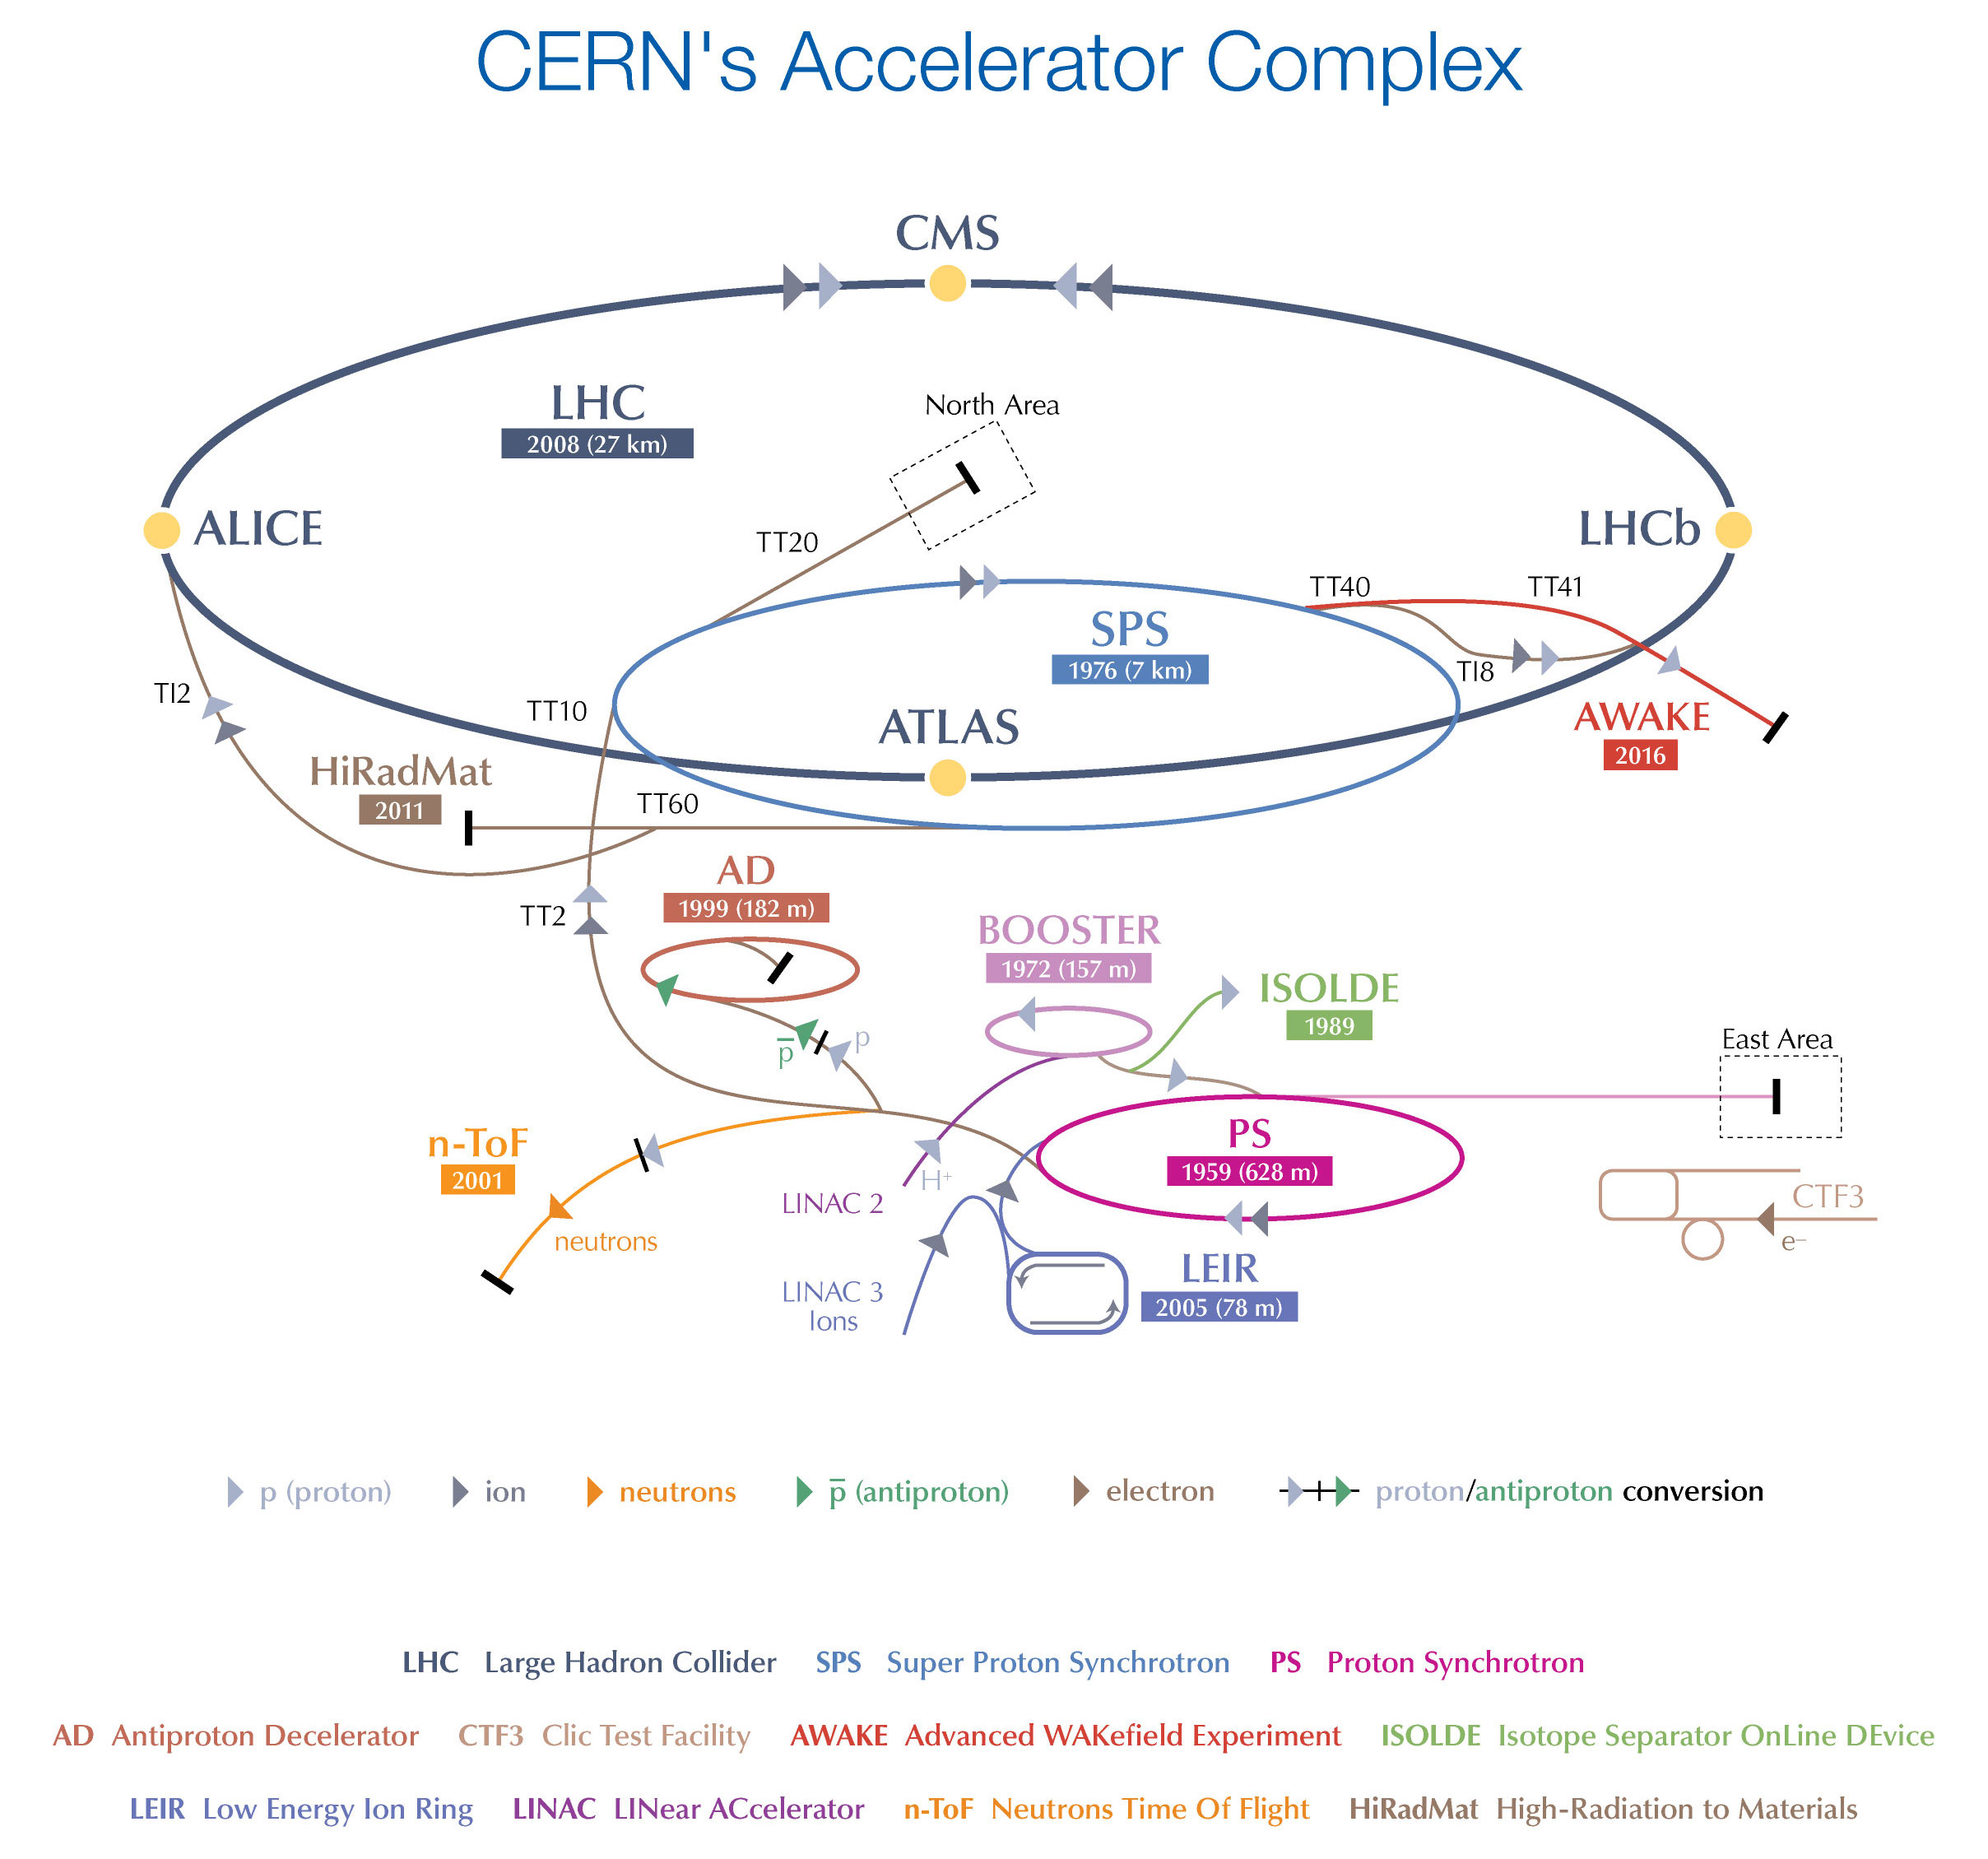
\includegraphics[width=0.9\textwidth]{Figures/CERNcomplex}
	\caption[The full \acrshort{cern} complex showing schematically the location of all the experiments on the ring complex, including the location of the four main experiments at the \acrshort{lhc}: \acrshort{cms}, \acrshort{atlas}, \acrshort{lhcb} and \acrshort{alice}.]{The full \acrshort{cern} complex showing schematically the location of all the experiments on the ring complex, including the location of the four main experiments at the \acrshort{lhc}: \acrshort{cms}, \acrshort{atlas}, \acrshort{lhcb} and \acrshort{alice}~\cite{CERNcomplex}. }
	\label{fig:CERNcomplex}
\end{figure}
% http://public-archive.web.cern.ch/public-archive/en/lhc/Facts-en.html

\section{The Large Hadron Collider}
\label{sec:LHC}

\subsection{A brief history of the \acrshort{lhc} and \acrshort{cms}}
\label{ssec:LHCHist}
% TODO move ref
All dates from the \acrshort{lhc} timeline are taken from~\cite{LHCtimeline}.
The first public announcement for the construction of the \acrshort{lhc} was given on the 16th December 1994. 
A couple of years earlier, on the 1st October 1992, the \acrshort{cms} experiment submitted its letter of intent to the \acrshort{lhc} Experiments Committee and on the 31st January 1997, the \acrshort{cms} experiment was approved.
Construction of the \acrshort{cms} site at Cessy began in July 1998, with the \acrshort{cms} cavern completed by the 1st February 2005.
In the following three years, the detector was assembled in segments above ground and lowered down into the cavern.
The final large detector segment was lowered on the 23rd July 2008.
The final dipole magnet of the \acrshort{lhc} was lowered into place on 26th April 2007, heralding the completion of the full accelerator ring.
The 10th September 2008, was a very significant day in the history of the \acrshort{lhc} marking the first circulation of proton beams around the collider. 
Shortly after, on the 19th, a fault occurred in an electrical connection between a dipole and quadrupole magnet, leading to a release of helium in the tunnels, causing significant damage to the \acrshort{lhc}. 
In total 37 damaged magnets were replaced and 16 refurbished, with the final one being lowered on the 30th April 2009. 
Beams were present again in the machine on the 20th November 2009, over a year after the malfunction. 

Run I physics data collection at a centre-of-mass energy $\sqrts=7\TeV$, was started on the 30th March 2010 and ran through until the 18th October 2011. 
A second period of data collection at $\sqrts=8\TeV$ was performed from the 5th April 2012 to the 6th February 2013. 
During this time, enough data was collected to confirm the existence of a \acrshort{sm}-like \Hboson{} boson, officially announced on the 4th July 2012~\cite{CMS:Higgs}.
With one of the primary mandates of the \acrshort{lhc} fulfilled, attention has turned to discovering the existence of physics beyond the \acrshort{sm} and measuring precisely the properties of the \Hboson{} boson and other \acrshort{sm} particles.

On the 3rd June 2015, after a two year long shutdown for upgrades, the collider started up again for Run II at an unprecedented $\sqrt{s}=13\TeV$. 
Four sets of data are scheduled to be taken during Run II, with a small set taken at the end of 2015 and major runs during 2016, 2017 and 2018.
Each major run lasts from a commissioning period around March to the end-of-year technical stop in December.
Run II data is scheduled to be collected until December 2018, from when it will enter a second long shutdown period before Run III scheduled to operate between 2020-2022.
This thesis uses the data set collected during 2016.

\subsection{Operating the \acrshort{lhc}}
\label{ssec:LHCoperation}

The source for the proton beams is a small canister of hydrogen gas. 
The hydrogen gas is then ionised to create protons by applying a large electric field.
The collection of protons is then accelerated, within ultra-high vacuums, through the \acrfull{linac}, which uses alternatingly charged conductors to accelerate the bunch of protons up to a beam energy of 50\MeV{}, before being injected into the \acrfull{psb}.
The \acrshort{psb} is an accelerator ring that boosts the protons to an energy of 1.4\GeV{} and passes them to the \acrfull{ps} which provides a further boost up to 25\GeV{}.
From the \acrshort{ps} the proton bunches are accelerated in the \acrfull{sps} to an energy of 450\GeV{}. 
The \acrshort{sps} splits the single beam into two counter-rotating ones and injects them into the \acrshort{lhc}.
In the \acrshort{lhc}, each proton beam can be accelerated up to a maximum energy of 7\TeV{} per beam. 
During Run I, the beam energy was operated at both 3.5 and 4\TeV{} and was increased to 6.5\TeV{} for Run II. 

To reach these operational collision energies the proton bunches are accelerated, confined and squeezed by magnetic fields of up to 8.3\Tesla{} from over 9300 superconducting magnets. 
The most common type of magnet used in the \acrshort{lhc} is the dipole magnet, of which there are 1232.
Each dipole magnet is 15\m{} long, weighs 35 tonnes and has a magnetic field strength of 8.3\Tesla{} which is used to bend the beam around the collider. 
Figure~\ref{fig:LHCdipole} shows a cross section through one of the \acrshort{lhc} dipole magnets.
Each dipole contains two beam pipes for the counter-circulating beams and along each of these beam pipes are coiled niobium-titanium alloy wires which form the superconducting dipole magnet. 
Superconductivity in the magnet is achieved by a closed circuit of liquid helium, which cools the iron yoke to 1.9\Kelvin{}.
\begin{figure}[htpb]
	\centering
	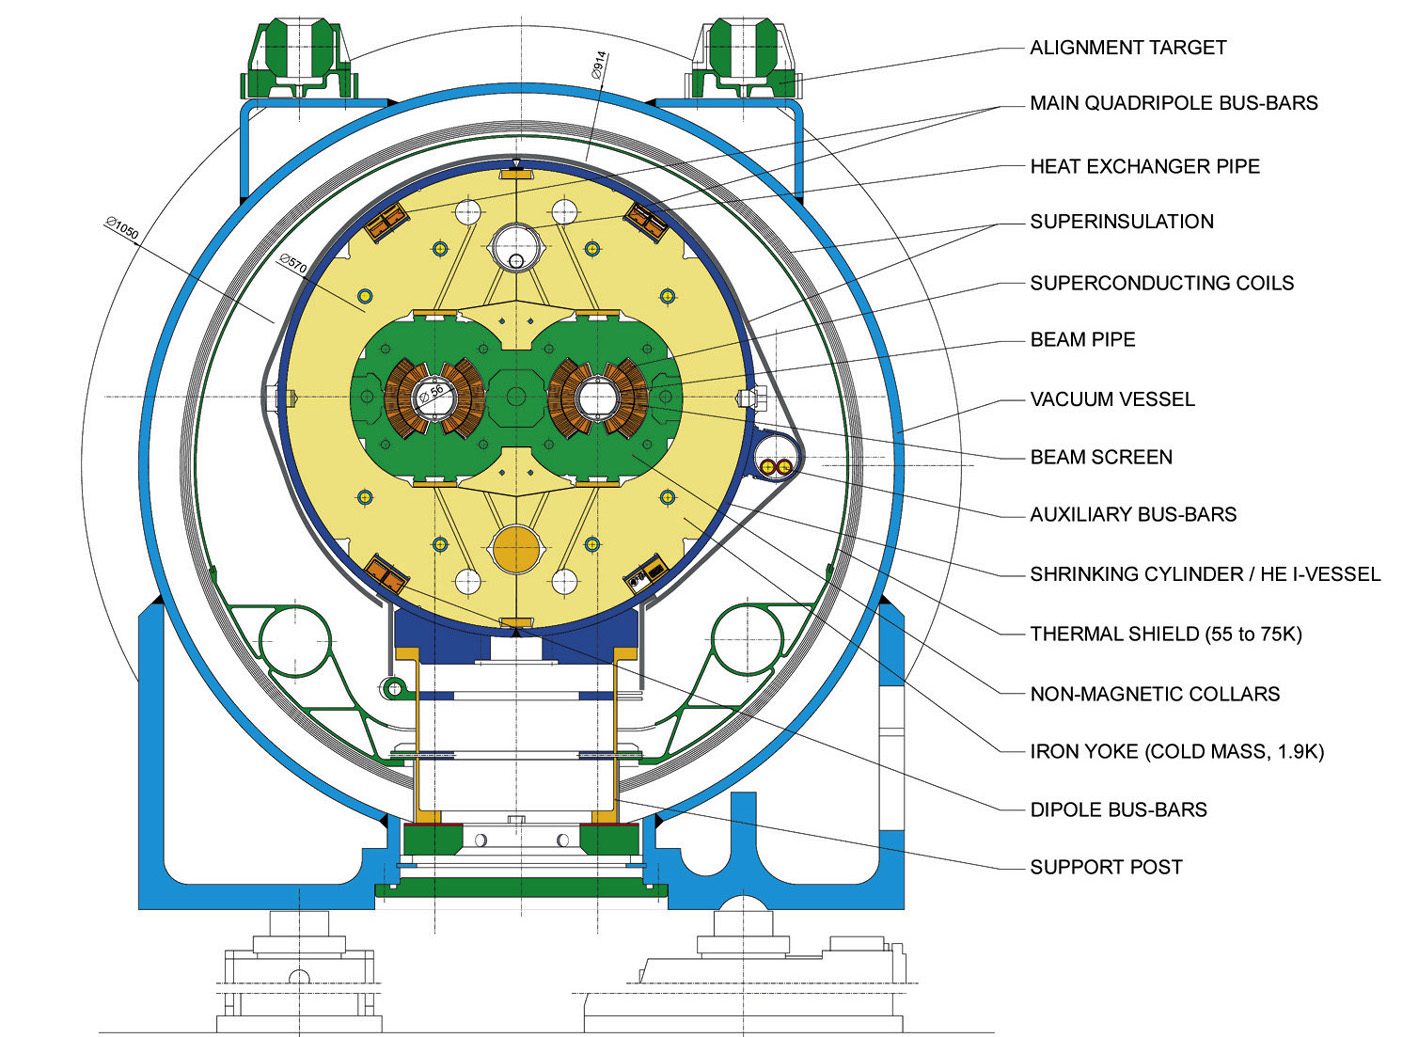
\includegraphics[width=0.8\textwidth]{Figures/LHCdipole}
	\caption[A cross section of a \acrshort{lhc} dipole magnet.]{A cross section of a \acrshort{lhc} dipole magnet~\cite{LHCdipolemagnet}. }
	\label{fig:LHCdipole}
\end{figure}
% Different specs for inner outer coils: http://lss.fnal.gov/archive/2015/conf/fermilab-conf-15-635-td.pdf
% Busbar = highvoltage power rail
% http://ieeexplore.ieee.org/stamp/stamp.jsp?arnumber=1211818

In addition to the dipole magnets, the \acrshort{lhc} uses 858 quadrupole magnets. 
Of these, 392 are lattice quadrupoles used to stop the beam from defocussing over time due to the similarly charged beam constituents. 
Quadrupole magnets are also used to confine the proton beams as they are entering the experimental caverns. A set of three, known as an inner triplet, squeezes each beam to a diameter of 16\um{} to ensure a maximal number of collisions at the interaction point.
There are additional multipole magnets used to correct for other, smaller, effects present in the beam, such as the gravitational force on the protons. 
% electromagnetic interactions among bunches, electron clouds from the pipe wall

\section{Luminosity measurements}
\label{sec:lumi}

The instantaneous luminosity is defined as:
\begin{equation}
\label{eq:InsLumi}
\Lum = f \frac{n_{1}n_{2}}{4\pi \sigma_{x} \sigma_{y}}
\end{equation}
\Lum{} depends on the bunch crossing rate, $f$, the number of protons in each colliding bunch, $n_{1}$ and $n_{2}$, and the root-mean-square of the transverse beam sizes in the horizontal ($\sigma_{x}$) and vertical ($\sigma_{y}$) directions. 
The beams are assumed to have a Gaussian profile, of width $\sigma=16\um$, and to be colliding head-on.
For nominal running during Run II, each beam contains 3564 bunch spaces of which typically 2808 are filled during data taking, leading to a minimum bunch spacing of 25\ns{} and a collision rate $f=40\MHz$.
Each bunch contains $\approx 1.1\ten{11}$ protons, producing a peak $\Lum=1.50\ten{34}\Lunit$.
\Lum{} varies with respect to time due to the depletion of the protons in each bunch after every collision.
The decrease in luminosity is mitigated to a small extent by the reduction of the beam widths $\sigma_{x}$ and $\sigma_{y}$, however each beam has an approximate physics taking lifetime of ten hours before they need to be refilled.
The total number of inelastic collisions (known as minimum bias events) produced at the \acrshort{lhc}, over a time $t$, can be estimated from the luminosity by:
\begin{equation}
\label{eq:nEvent}
\text{N} = \sigma_{\text{minbias}}\times\Lum_{\text{int}}, 
\end{equation}
where $\sigma_{\text{minbias}}$ is the minimum bias cross section.
$\Lum_{\text{int}}$ is the integrated instantaneous luminosity over time $t$
\begin{equation}
\label{eq:IntLumi}
\Lum_{\text{int}} = \int^{t}_{t_{0}}\Lum(t)\text{d}t.
\end{equation}
The $\Lum_{\text{int}}$ distribution during the 2016 data taking period is shown in the upper panel of Fig.~\ref{fig:CMSLumi}, where a total of \Lumi{} of certified data was collected by the \acrshort{cms} experiment.
The lower panel shows the delivered luminosity for all other years of data taking.
Using the current $\sigma_{\text{minbias}}$ measurement of 69.2\mb{}, this means that approximately $2.5\ten{15}$ collisions were processed in this period.
\begin{figure}[htpb!]
	\centering
	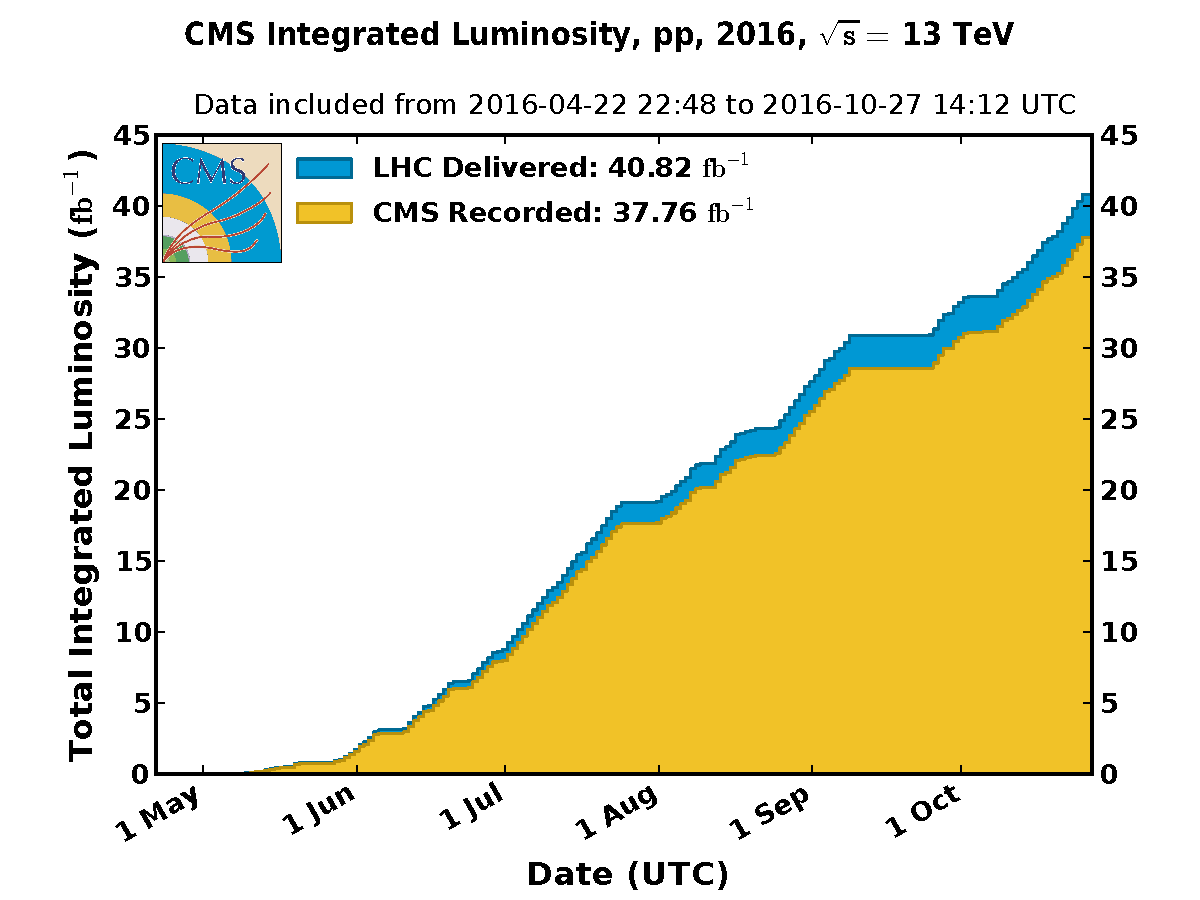
\includegraphics[width=0.85\textwidth]{Figures/LHC2016Lumi} \\
	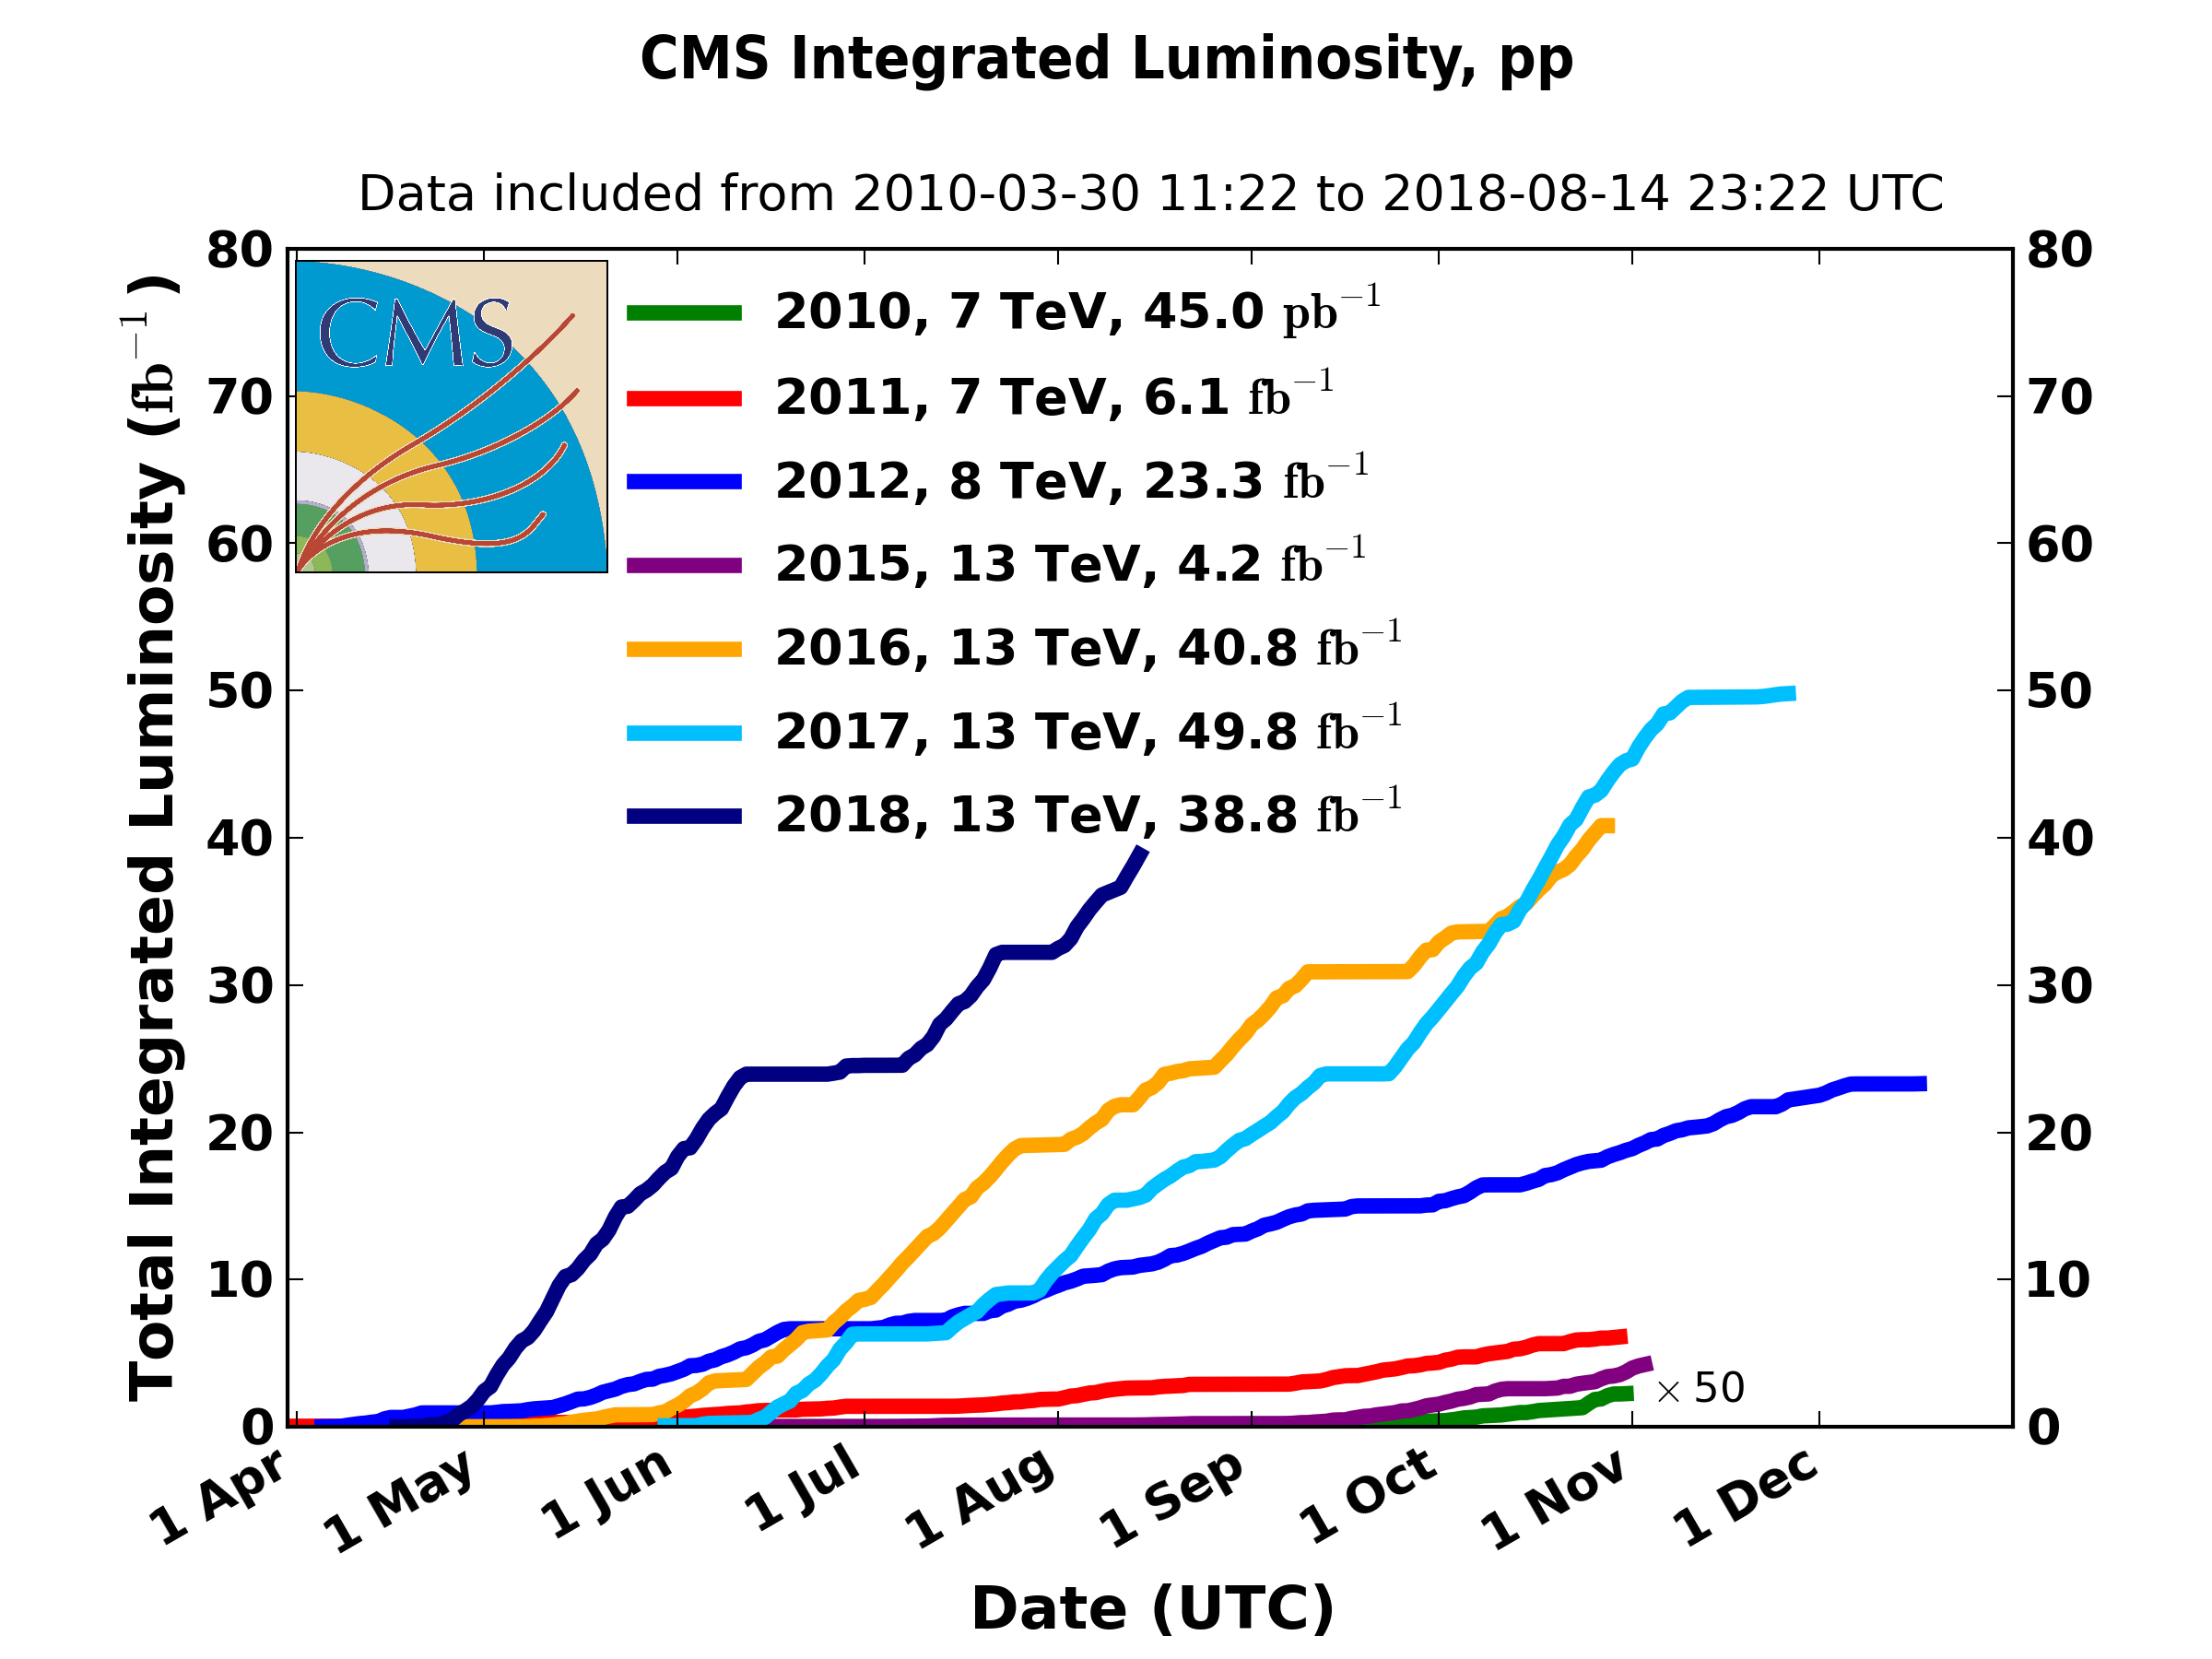
\includegraphics[width=0.85\textwidth]{Figures/LHCLumiAllYears}
	\caption[The upper panel shows the delivered and recorded integrated luminosity during data taking in 2016 and the lower panel the integrated luminosity delivered by the \acrshort{lhc} for all years of operation.]{The upp panel shows the delivered and recorded integrated luminosity during data taking in 2016 and the lower panel the integrated luminosity delivered by the \acrshort{lhc} for all years of operation. Figures taken from~\cite{CMS:CMSLumi}.}
	\label{fig:CMSLumi}
\end{figure}

More than one proton-proton interaction typically occurs in each bunch crossing and these additional interactions are referred to as \textit{in-time pileup}.
As the collision rate at the \acrshort{lhc} is so high, it is also possible for remnants of previous bunch crossings to affect the current one, particularly in calorimeters where there is a latency higher than a typically bunch spacing.
These remnants are called \textit{out-of-time pileup}.
The average number of interactions per bunch crossing during 2016 data taking was approximately 30, as can be seen in Fig.~\ref{fig:CMSPU}, using a minimum bias cross section of $80\mb$.
Particles from pileup are included in the particle reconstruction of the event, leading to misidentification.
Reconstruction and pileup mitigation techniques are described in Secs.~\ref{ssub:antikt} and~\ref{sub:jet_energy_corrections}.
\begin{figure}[htpb]
	\centering
	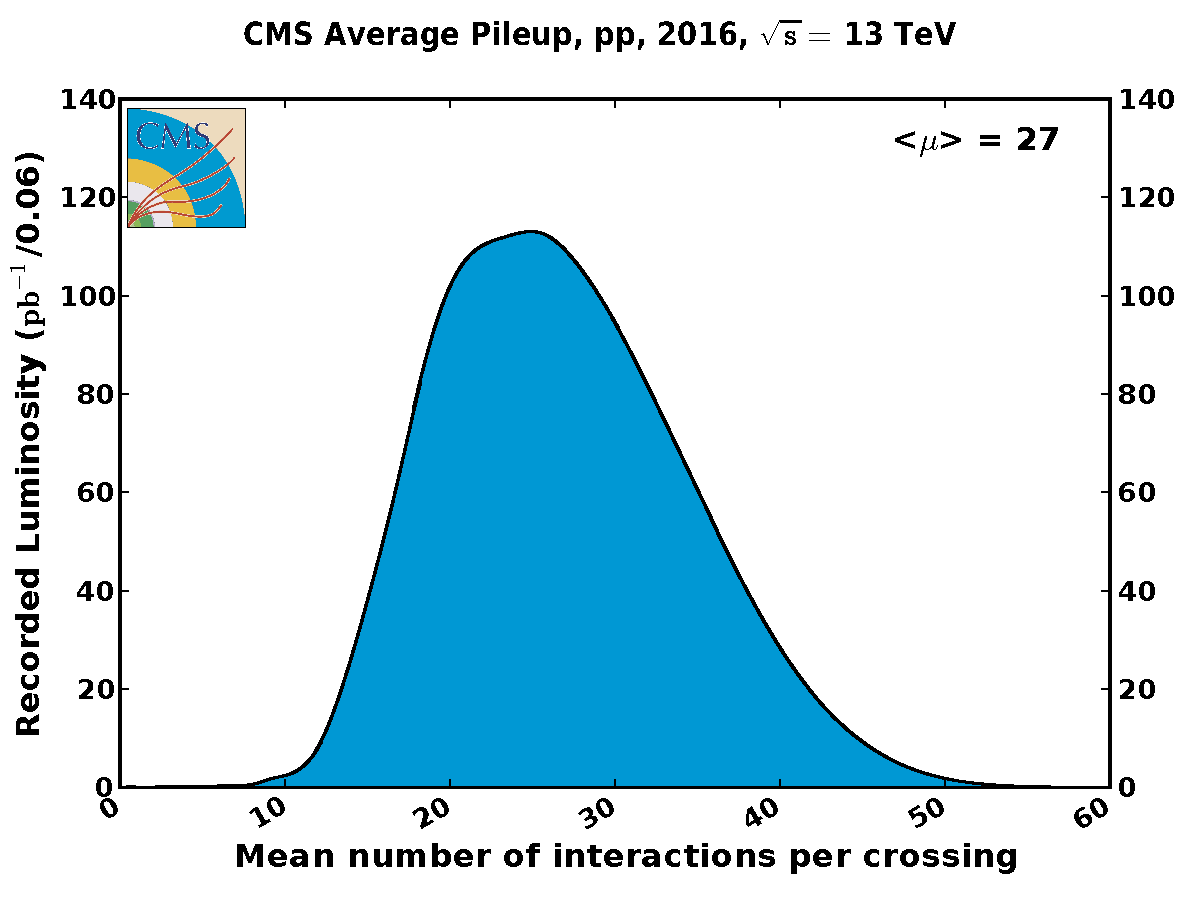
\includegraphics[width=0.8\textwidth]{Figures/CMSAvePU}
	\caption[The distribution of the number of interactions in a bunch crossing. The minimum bias cross section is taken to be $80\mb$.]{The distribution of the number of interactions in a bunch crossing. The minimum bias cross section is taken to be $80\mb$. Figure taken from~\cite{CMS:CMSLumi} }
	\label{fig:CMSPU}
\end{figure}

% sigma^2 (beam size) = epsilon.beta* (emittance . beta function)
% emittance – the spatial and angular spread of particles. A low emittance particle beam is a beam where the particles are confined to a small distance and have nearly the same momentum.
% Link to Tracker - lots of particles need high granularity tracker.
% Not quite head on collisions add another crossing angle factor
% 1.15 is design, 1.1 is actual http://accelconf.web.cern.ch/accelconf/hb2016/papers/moam5p50.pdf
% 27km / 3564b / 3e8 = 25ns :D
% Check

\section{The Compact Muon Solenoid}
\label{sec:CMS}

\acrshort{cms} is a general purpose detector, designed to be able to perform precision measurements of the standard model and searches for new physics~\cite{CMSExperiment}. 
It is a cylindrical, hermetic detector composed of a barrel region and two endcaps, each formed of layers of subdetectors around the beam collision point, as shown in Fig.~\ref{fig:CMSPicture}. 
These subdetectors, in order from the collision point, are the pixel and strip tracker, electromagnetic calorimeter (\acrshort{ecal}), hadronic calorimeter (\acrshort{hcal}) and muon chambers.
The superconducting magnet is situated in between the hadronic calorimeter and muon chambers.
To operate in a high luminosity environment the \acrshort{cms} experiment must have excellent resolution in each of its subdetectors and a low latency to manage the high collision rate. 
The materials used must be reliable while having maximal longevity when operating in a high-radiation environment.

\acrshort{cms} uses a right-handed coordinate system, where the $x$-axis points towards the centre of the accelerator ring, the $y$-axis points vertically upward and the positive $z$-axis lies parallel to the anti-clockwise beam axis. 
The azimuthal angle $\phi$, is measured from the $x$-axis in the transverse $x-y$ plane. 
The polar angle $\theta$, is measured from the positive $z$-axis in the $z-y$ plane.
At the \acrshort{cms} experiment, collisions are viewed in the centre-of-mass frame of the colliding protons, which means that the colliding partons usually have a Lorentz boost along the beam direction.
For this reason, the angles of the particles are normally expressed in terms of the rapidity ($y$) or pseudorapidity ($\eta$), in which the production is roughly constant.  
The rapidity is defined as
\begin{equation}
\label{eq:rap}
y\equiv {\frac{1}{2}}\ln\left({\frac{E+p_{z}}{E-p_{z}}}\right),
\end{equation}
where $E$ is the energy of a measured particle and $p_{z}$ is the $z$-component of the momentum.
Rapidity is advantageous to use as rapidity differences between two particles is invariant under a Lorentz boost along the $z$-axis.
At the \acrshort{lhc}, most particles are highly relativistic such that the rest mass is small compared to the energy ($p_{z}\approx E\cos\theta$). This can be substituted into Eq.~\ref{eq:rap} and using trigonometric relations, the pseudorapidity is defined as
\begin{equation}
\label{eq:eta}
\eta \equiv -\ln\left(\tan\left({\frac{\theta}{2}}\right)\right).
\end{equation}

% Henceforth, angular measurements are given in terms of pseudorapidity.
Jet production in \pp{} collisions is roughly constant in $\eta$, reflecting the forward nature of the production.
The subdetectors at the \acrshort{cms} experiment extend to at least a pseudorapidity magnitude of 2.4, covering more than 95\% of the phase space. 
Individual subdetectors can extend to a higher $\abs{\eta}$, for example the forward detectors of the \acrshort{hcal}, to study very boosted jets or the underlying event.
The acceptance within $\abs{\eta} < 2.4$ can be hampered by issues such as the gap between barrel and endcap detectors.
% 2.4 => 10deg. 1 str=33 deg. lost=0.61str. pc = 4.8

To completely describe the kinematic properties of a particle, its energy and momentum must be known. 
While it is not possible to detect the complete momenta spectrum of an event, due to many particles produced in the collision being lost down the beam pipe and the unknown boost of the partons, it is possible to measure the momenta in the transverse plane, where the sum of the momenta is conserved. 
To measure the transverse momenta and energy of particles, \acrshort{cms} uses a combination of hits in the tracking systems from charged particles and energy deposits in the calorimeters.
These subsystems are described in more detail in the following sections.

% \begin{landscape}
% \centering
\begin{figure*}[htpb]
	\centering
	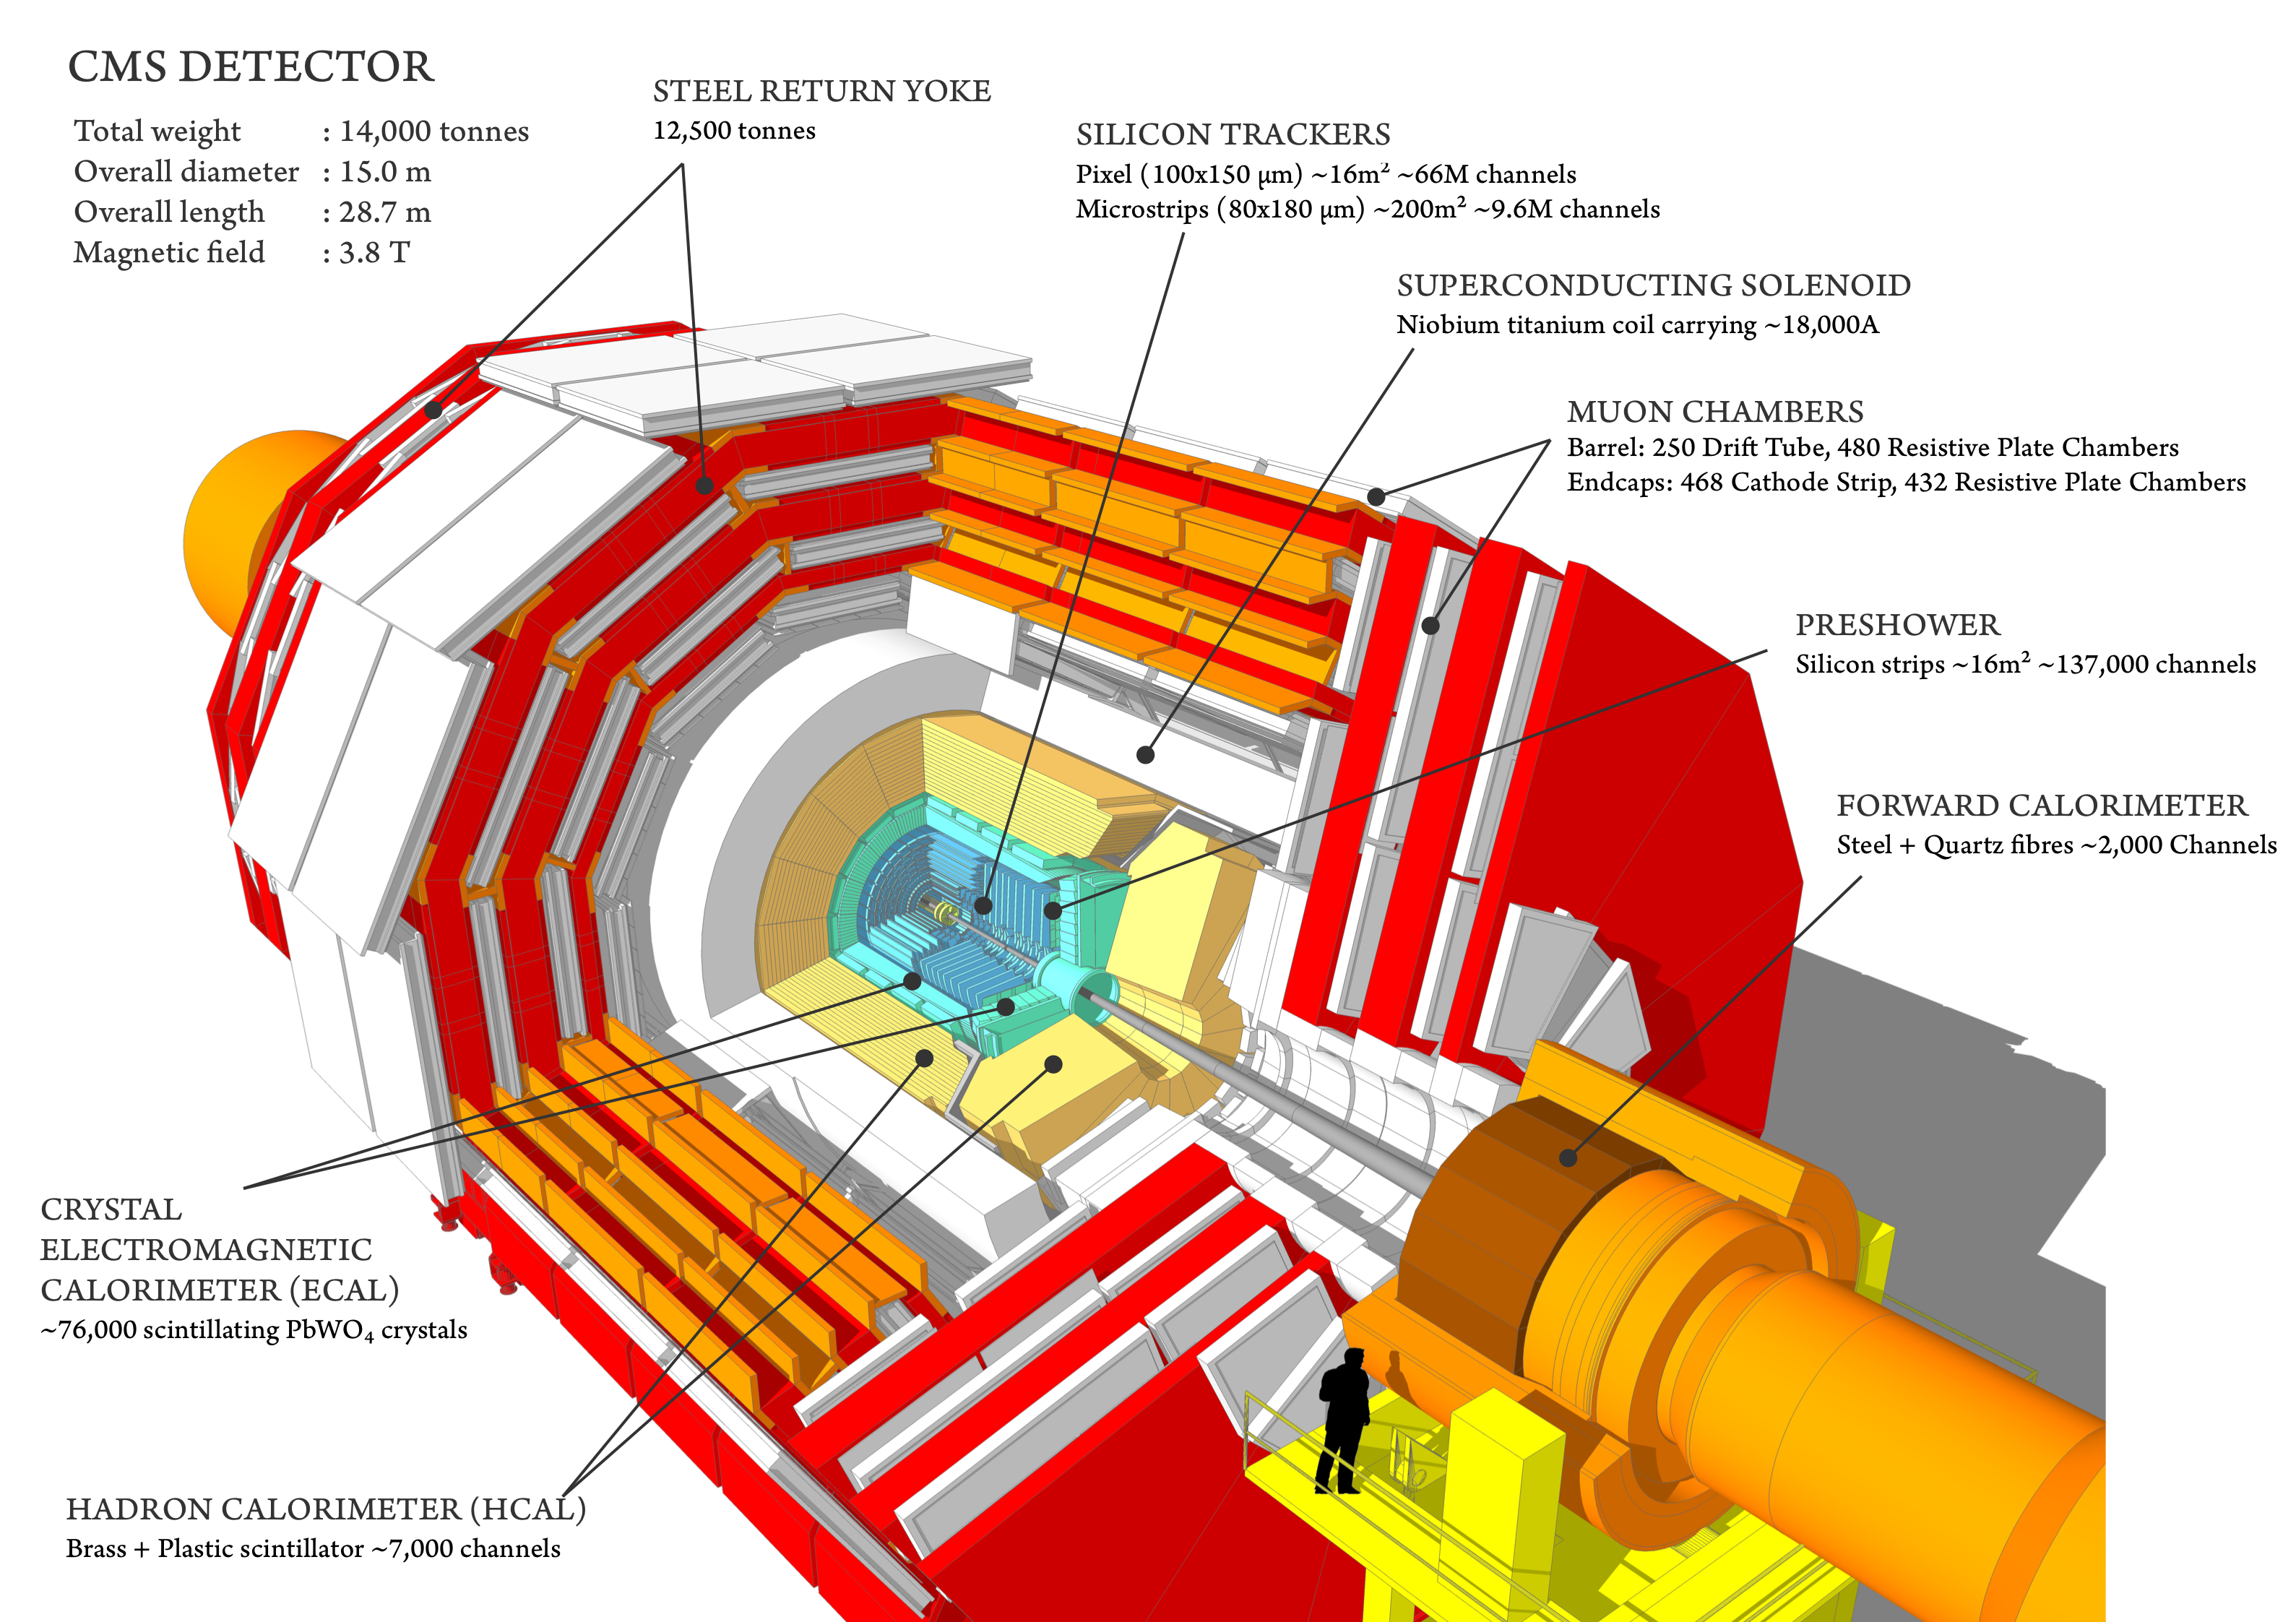
\includegraphics[width=\linewidth]{Figures/CMSPicture}
	\caption[A schematic of \acrshort{cms}, sliced to show the internal layout. It consists of layers around the central interaction point in the order of silicon pixel and strip detectors, electromagnetic and hadronic calorimeters, superconducting magnet and finally muon chambers. ]{A schematic of \acrshort{cms}, sliced to show the internal layout. It consists of layers around the central interaction point in the order of silicon pixel and strip detectors, electromagnetic and hadronic calorimeters, superconducting magnet and finally muon chambers~\cite{CMSPicture}.}
	\label{fig:CMSPicture}
\end{figure*}
% \end{landscape}

\subsection{\acrshort{cms} pixel and strip trackers}
\label{ssec:Tracker}
% Page 62

Figure~\ref{fig:CMSTracker} shows the layout of the silicon tracking detectors in \acrshort{cms}. 
Closest to the interaction point are the pixel detectors consisting of three barrel layers situated at radial distance $r=4.4, 7.3$ and 10.2\cm{} in the transverse plane from the interaction point with two endcap disks lying at $z=\pm34.5$ and $\pm46.5\cm$.  
There are 65 million pixels in the inner tracker, each $100\times150\umsq$, giving a total active area of 1.06\msq{}.
Surrounding the pixel detectors are the silicon strip tracker sensors. 
These are arranged into four subsystems: the Tracker Inner Barrel and Disks (\acrshort{tib} and \acrshort{tid}s), the Tracker Outer Barrel (\acrshort{tob}) and the Tracker Endcaps (\acrshort{tec}s).
The \acrshort{tib} consists of four barrel layers between $20<r<55\cm$ with each end capped by 3 disks ($|z|<118\cm$) forming the \acrshort{tid}s. 
Wrapping around the \acrshort{tib} and \acrshort{tid}s is the \acrshort{tob} consisting of six barrel layers between $55<r<116\cm$. 
Finally, each \acrshort{tec} consists of nine disks between $124<|z|<282\cm$, capping the \acrshort{tib}, \acrshort{tid}s and \acrshort{tob}.
There are $15\,148$ silicon strip modules in total that make up the outer tracker, giving a total active surface area of 198\msq{}. 
Some strip layers in the tracker, coloured blue in Fig.~\ref{fig:CMSTracker}, have back-to-back modules, rotated with respect to each other by a small stereo angle ($\approx5\de$) in order to improve the 3-dimensional point resolution by providing a measurement of the $z$ co-ordinate in the barrel and $r$ in the disks.

\begin{figure}[htpb]
	\centering
	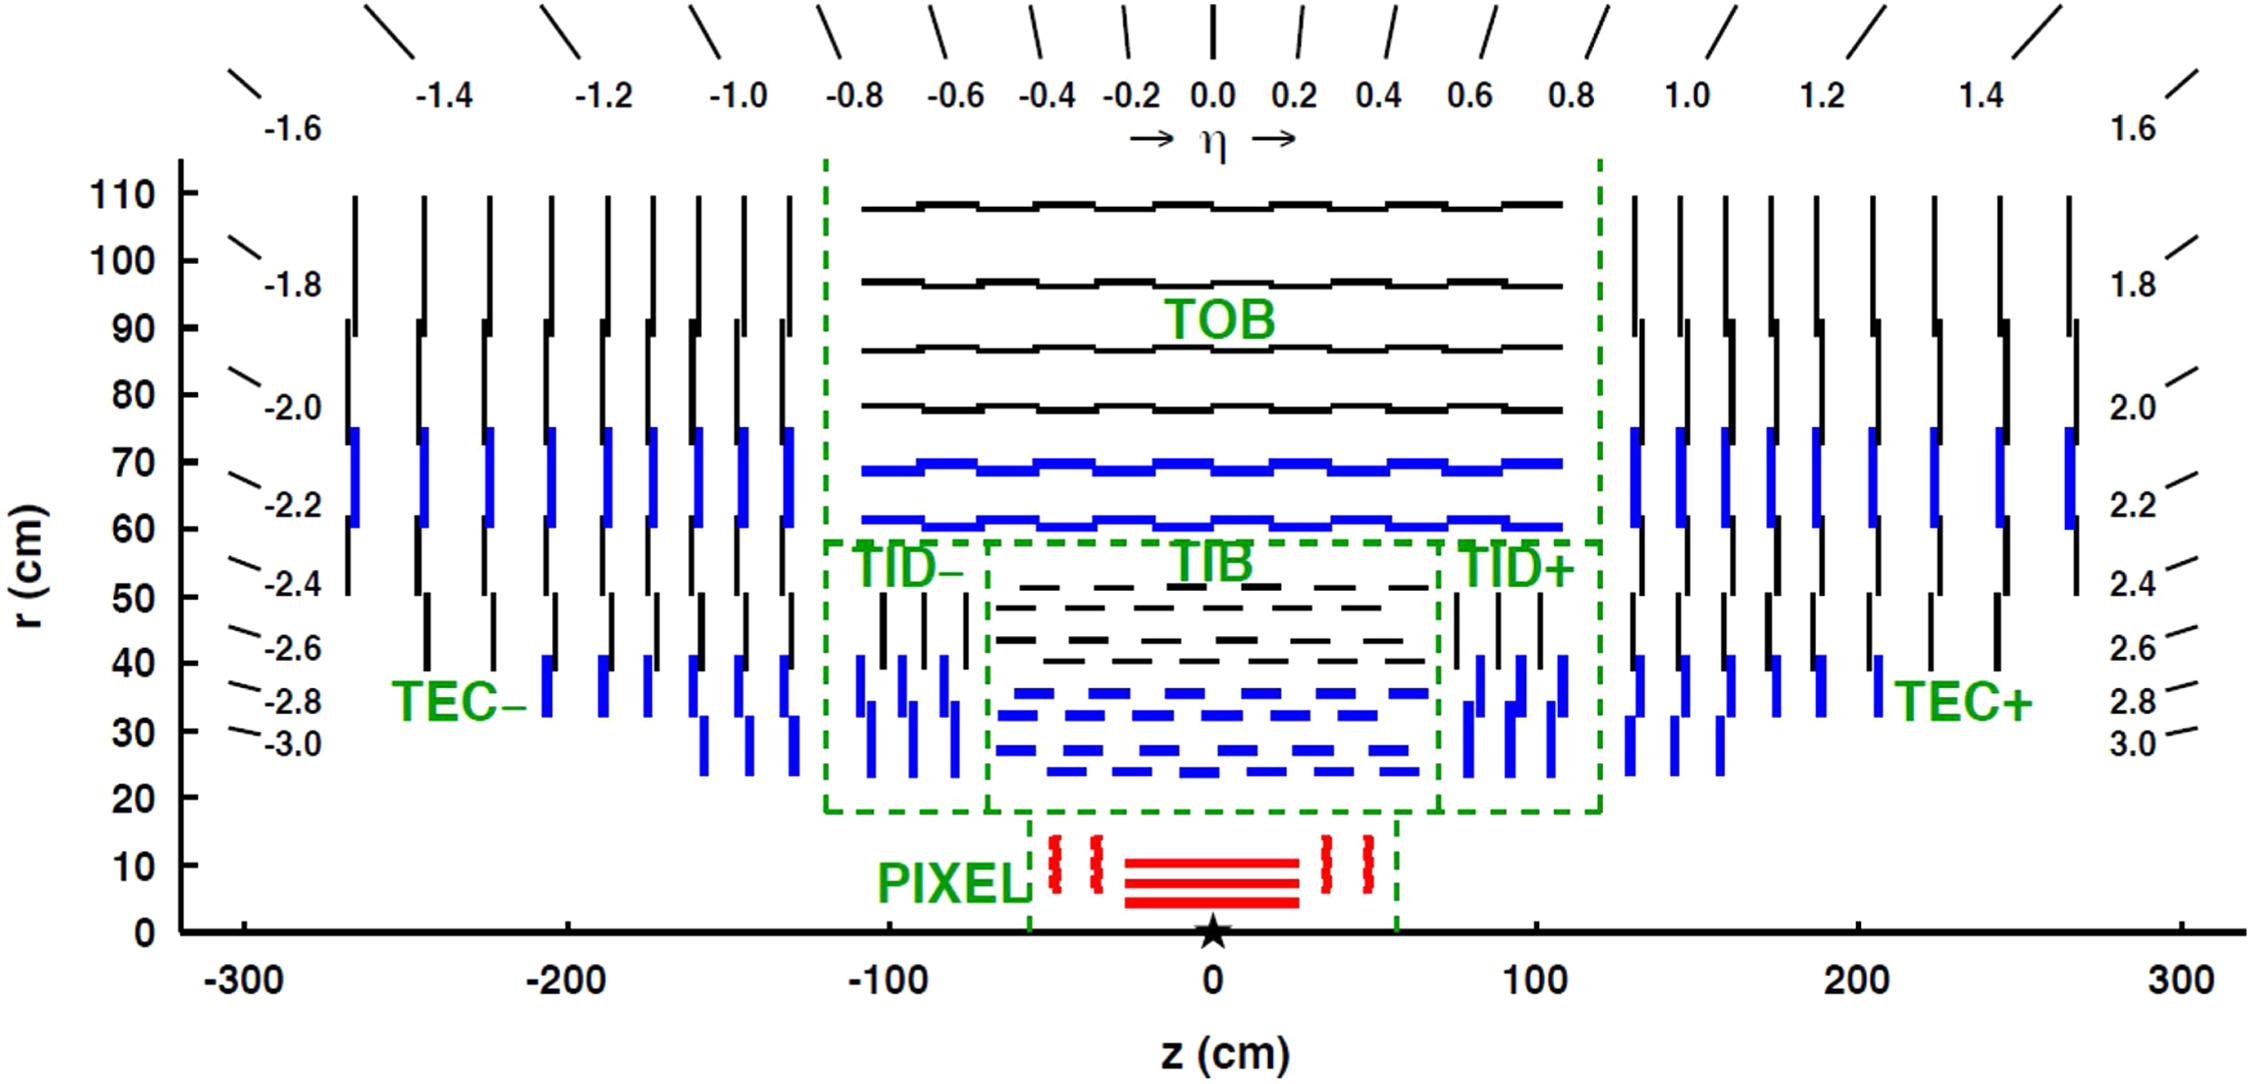
\includegraphics[width=\textwidth]{Figures/CMSTracker2.jpg}
	\caption[A slice through the \acrshort{cms} tracker detector in the $r-z$ plane. The separate subsystem regions have been highlighted and are classified as the Tracker Inner Barrel and Disks (\acrshort{tib} and \acrshort{tid}s), the Tracker Outer Barrel (\acrshort{tob}) and the Tracker Endcaps (\acrshort{tec}s). The Pixel subsystem is highlighted in red. Back-to-back stereo strip modules are highlighted in blue.]{A slice through the \acrshort{cms} tracker detector in the $r-z$ plane. The separate subsystem regions have been highlighted and are classified as the Tracker Inner Barrel and Disks (\acrshort{tib} and \acrshort{tid}s), the Tracker Outer Barrel (\acrshort{tob}) and the Tracker Endcaps (\acrshort{tec}s). The Pixel subsystem is highlighted in red. Back-to-back stereo strip modules are highlighted in blue. Figure taken from~\cite{CMSTrackerPerformance}.}
	\label{fig:CMSTracker}
\end{figure}
% of size $100\times150$ $\mu m^{2}$, uses 

Each tracking sensor operates in a similar manner.
For the pixel sensors, an \nnjunc{} junction is utilised where the silicon has been doped with phosphorous to different degrees. 
For the strip sensors, a \pnjunc{} junction is used where a silicon strip doped with boron has been laid on the bulk n-type silicon.
Doping with phosphorous causes the silicon to become an electron donor (n-type) and doping with boron to become an electron acceptor (p-type).
The n(p)$^{+}$-type silicon is where silicon has been doped to such an extent that the resistivity is very low.% resulting in a very good chip readout connection.

In the case of the silicon strip sensor, electrons diffuse from the bulk n-type silicon to a strip of p$^{+}$-type silicon, creating a small opposing electric field from the formation of ions either side of the \pnjunc{} junction.
The field stops further electron-hole movement and forms a potential step.
The region with no excess electrons or holes is known as the depletion zone, which causes the junction to act as a diode.
A reverse bias voltage is applied to ensure the silicon is fully depleted by attracting the free electrons and holes away from the \pnjunc{} junction.
% A reverse bias voltage is applied to counteract this electric field, increasing the size of the stable depletion zone.
% The reverse bias voltage causes the p$^{+}$-type silicon strip to act as a diode, cutting any... TODO.
When a charged particle ionises the n-type bulk silicon, the electrons and holes produced ($\approx 30\,000$) drift in the large electric field such that the holes move towards the p$^{+}$-type silicon producing a small signal current which is then amplified and shaped.
This method can be applied to any semiconductor junction where each side has different doping concentrations.

% http://ieeexplore.ieee.org/stamp/stamp.jsp?arnumber=4774788
The pixel detector receives a charged particle flux of $1\MHz\mmsqinv$. 
At this high rate of particles the pixels must have a high granularity to keep the fraction of channels hit (occupancy) reasonable.
A low occupancy in the pixel detector is necessary to reconstruct individual particle tracks back to an interaction vertex, in a high-track environment.
Lower occupancies present in the \acrshort{tob} and \acrshort{tec}s mean that a longer strip can be used, however this incurs an increase in noise, which is alleviated by increasing the thickness of the silicon sensor from 320\um{} to 500\um{}.
Tracks reconstructed in the pixel and strip detectors can then be used in vertex reconstruction, particle identification and charged particle momenta measurements.
The track reconstruction is detailed in Sec.~\ref{sub:Particle_flow_elements}.
% TODO APV
% TODO Endcap turbine shape - due to Lorentz drift in non uniform magnetic field.

% Both the pixel and tracker use the same bulk silicon.

% A total of TODO sensors are used in the pixel and tracker...
% The electrons and holes drift in opposite directions due to a TODOkV applied electric field (TODO the bias voltage).
% The current created by the electrons and holes is readout from the sensor
% p = Nholes, n = nElectrons
% https://cds.cern.ch/record/2282804/files/thesis.pdf


% pn junction - depletion zone holes <--> electrons. Creates small electric field opposing further drift and diffusion. Stable area. Made bigger or smaller by applying Pot Diff. Forward bias is smaller DZ, Rear Biased is larger. Want larger... -> low leakage current. Charged particle passes leaving 30000eh pairs
% https://www.hephy.at/fileadmin/user_upload/Halbleiterdetektoren.pdf

% \subsubsection{New Pixel Detector}
% \label{sssec:Tracker}
% Include the new 2017 Pixel detector?

\subsection{Electromagnetic calorimeter}
\label{ssec:ECAL}
% http://cms.web.cern.ch/news/crystal-calorimeter
% https://arxiv.org/pdf/1306.2016.pdf
% Moliere Radius: The radius of a cyclinder which contains 90% of the EM showers energy deposition. Smaller Moliere radii mean better shower spatial resolution and better shower separation due to smaller degree shower overlaps.
% Radiation Length: 

The \acrshort{cms} \acrshort{ecal}, as shown in Fig.~\ref{fig:CMSECAL}, is made of three subsystems: the barrel, the endcaps and the preshower detector.
Together, they form a compact coverage around the interaction point, up to $\abseta<3$.
\begin{figure}[htpb]
	\centering
	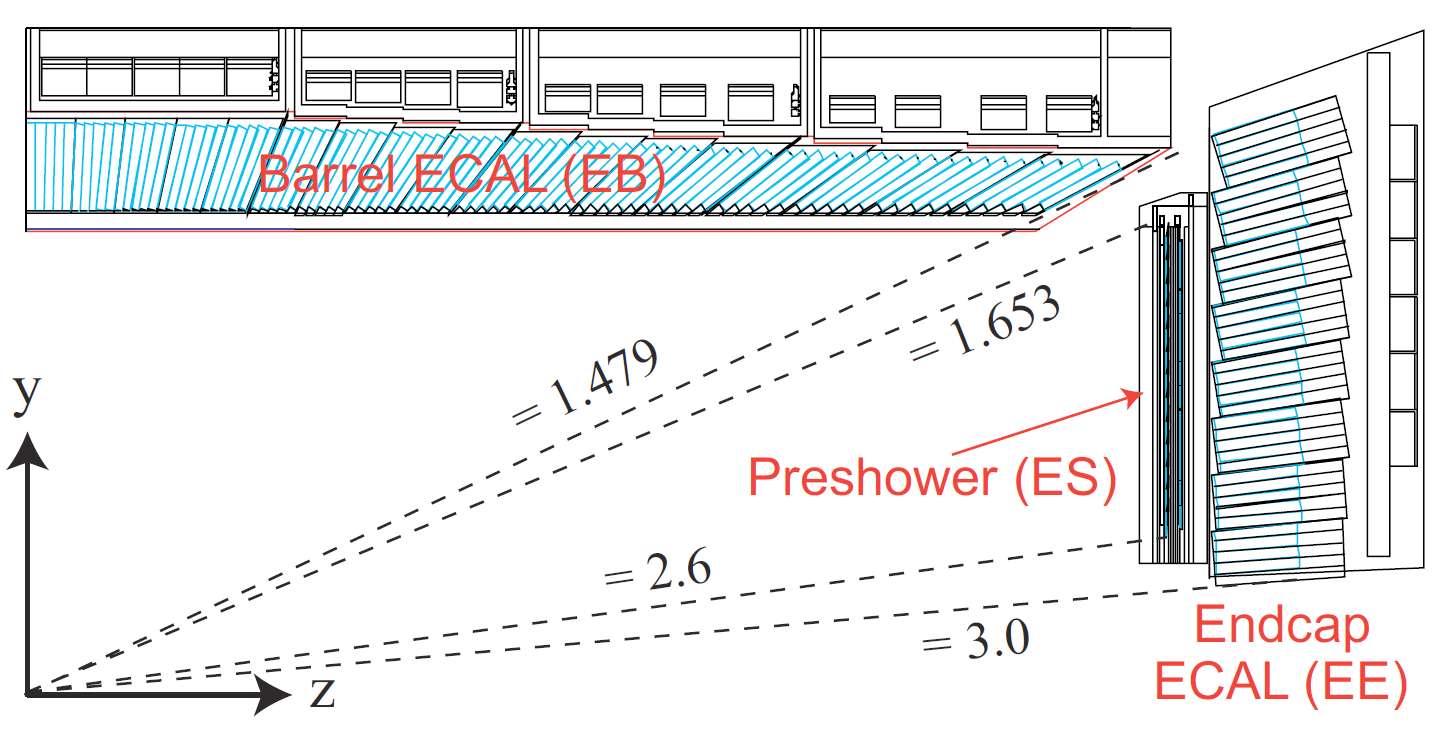
\includegraphics[width=\textwidth]{Figures/CMSECAL2}
	\caption[A geometrical quarter view of the \acrshort{cms} \acrshort{ecal}, highlighting the barrel, endcap and preshower detector regions.]{A geometrical quarter view of the \acrshort{cms} \acrshort{ecal}, highlighting the barrel, endcap and preshower detector regions. Figure taken from~\cite{CMSTDRV1}.}
	\label{fig:CMSECAL}
\end{figure}
% http://cms-project-ecal-p5.web.cern.ch/cms-project-ECAL-P5/approved/detector.htm
A total of $75\,848$ lead tungstate (\PbWO{}) scintillating crystals are used in the \acrshort{ecal} barrel and endcaps.
In the barrel section, the crystals are laid out in an $\eta-\phi$ grid extending to $\abseta<1.479$.
The inner surface of the barrel is at $r=1.29\m$, with each crystal having a front surface area of $2.2\times2.2\cmsq$ and length 23\cm{}.
In each endcap, the crystals are instead laid out in a $x-y$ grid, with the front surfaces at $z=\pm 3.14\m$, extending through $1.479 < \abseta < 3.0$. 
Each endcap crystal has a front surface area of $2.9\times2.9\cmsq$ and a length of 22\cm{}.
All the crystals are slightly off-centre with respect to the primary interaction point to avoid particles being lost down the small gaps between adjacent crystals.

\PbWO{} is an ideal choice for the \acrshort{cms} \acrshort{ecal} due to its short radiation and Moli\`ere lengths of 0.89 and 2.2\cm{} respectively. 
The radiation length gives a measure of the penetration of the \acrshort{em} shower into the crystal and the Moli\`ere length how confined the \acrshort{em} shower is, such that a cascade will mostly be contained within one crystal. 
In addition, \PbWO{} crystals are very fast with 80\% of the blue-green scintillation light being emitted in the time it takes for another collision to occur.
The light emission from the \PbWO{} crystals is relatively small at 30\photon{} per\MeV{} of energy deposited and therefore needs to be amplified using silicon avalanche photodiodes (barrel) and vacuum phototriodes (endcaps).
\PbWO{} is also radiation resistant tolerating up to $6.2\ten{17}\MeV\pow{kg}{-1}$ of radiation energy.
% 0.1\unit{MGy}.
% 0.1MGy = 100000 joule/kg
% What the hell are the APD and VPT and how do they work?
% 1 Gray = one joule of radiation energy per kilogram of matter

The purpose of the \acrshort{ecal} preshower detector is to distinguish between a high energy single photon and a $\pi^{0}$ decaying into two closely spaced photons.
To do this the preshower consists of two layers of lead, which initiate an electromagnetic shower for photons (and electrons), each closely followed by a layer of silicon strip detectors. 
The silicon strips are placed orthogonal to each other to measure shower positions precisely and are fine enough in granularity to differentiate between a single photon shower and multiple close-spaced photons.
A $\pi^{0}$ decaying in the barrel typically has low enough energy not to need the additional resolution provided by the preshower detector. 
The preshower degrades the resolution of the \acrshort{ecal} endcap due to the dense lead plates, however as the energy deposited within the lead is proportional to that deposited in the silicon, a correction can be applied mitigating the effect.
% http://www.hephy.at/project/cms/trigger/globalTrigger/trans/MEDIEN/Publications/CMSBooklet/Info_for_CMSBooklet/PreshowerFAQ_files/CMS3d.html

These attributes mean that the \acrshort{ecal} can be both compact enough to fit within the magnet and granular enough to perform with high energy resolution.
The resolution performance is measured by fitting a Gaussian function to the reconstructed energy distributions at different test beam energies and is parametrised by
\begin{equation}
	\left(\frac{\sigma_{\mathrm{ECAL}}}{E}\right)^{2} = \left(\frac{S}{\sqrt{E}}\right)^{2} + \left(\frac{N}{E}\right)^{2} + C^{2},
\end{equation}
where $S$ is a stochastic term (number of photoelectrons), $N$ is a noise term (electronics and digitisation) and $C$ is a constant term (leakage from the back of the \acrshort{ecal}).
% stochastic: having a random probability distribution or pattern that may be analysed statistically but may not be predicted precisely.
% S: statistical based, photoelectrons
% N: electronics. digitization
% C: leakage, nonuniformities in crystal
Figure~\ref{fig:CMSECALRes1} shows the energy resolution with respect to the energy deposited in a $3\times3$ crystal lattice around incident electrons at a test beam measurement before the beginning of Run I with the values for $S$, $N$ and $C$ shown. 
Figure~\ref{fig:CMSECALRes2} shows the energy resolution with respect to $\abs{\eta}$ from the most recent public measurement~\cite{CMSECALRESMEAS}.
It is extracted from an unbinned likelihood fit on $Z\rightarrow e^{+}e^{-}$ events collected in 2015 for electrons with low brehmstrahlung radiation and $\ET\approx45\GeV$.
The resolution was measured to be $<2\%$ for $\abseta<1.0$ and between $2-5\%$ elsewhere.
\begin{figure}[hpb!]
	\centering
	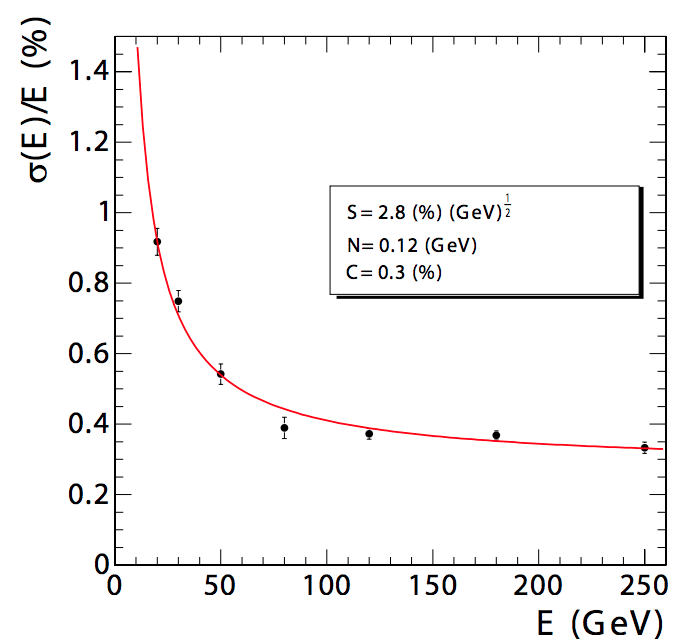
\includegraphics[width=0.6\textwidth]{Figures/CMSECALRES} \\
	\caption[The energy resolution of the \acrshort{cms} \acrshort{ecal} measured in a beam test. The energy was measured in a $3\times3$ crystal lattice with the electron striking the central crystal. ]{The energy resolution of the \acrshort{cms} \acrshort{ecal} measured in a beam test. The energy was measured in a $3\times3$ crystal lattice with the electron striking the central crystal. Figure taken from~\cite{CMSExperiment}.}
	\label{fig:CMSECALRes1}
\end{figure}
\begin{figure}[hpb!]
	\centering
	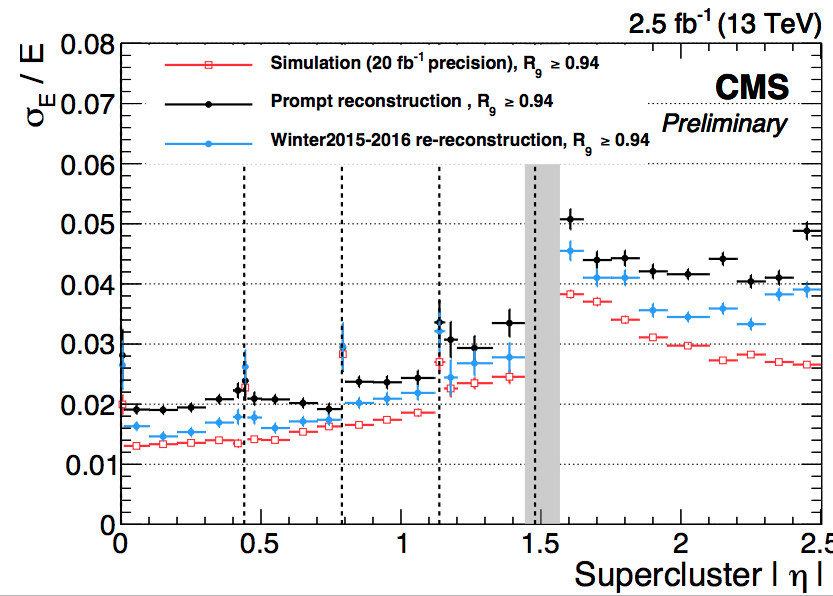
\includegraphics[width=0.8\textwidth]{Figures/CMSECALRES2}
	\caption[The energy resolution of the \acrshort{cms} \acrshort{ecal} extracted from an unbinned likelihood fit on $Z\rightarrow e^+e^-$ events.]{The energy resolution of the \acrshort{cms} \acrshort{ecal} extracted from an unbinned likelihood fit on $Z\rightarrow e^+e^-$ events. Figure taken from~\cite{CMSECALRESMEAS}.}
	\label{fig:CMSECALRes2}
\end{figure}
% Not public measurements at 13TeV?

% 61200 in the barrel, 7324 in each endcap 
% Each crytal covers 0.0174 (1deg) in phi and eta.
% Actually 2.86 cm.
% Barrel is structured as 36 identical “supermodules,” each covering half the barrel length and corresponding to a pseudorapidity interval of 0 < |η| < 1.479. The crystals are quasi-projective (the axes are tilted at 3◦ with respect to the line from the nominal vertex position) ∆η. 
% The endcaps (EE), at a distance of 314 cm from the vertex and covering a pseudorapidity range of 1.479 < |η| < 3.0, are each structured as 2 “Dees”, consisting of semi-circular aluminium plates from which are cantilevered structural units of 5×5 crystals, known as “supercrystals.”


\subsection{Hadronic calorimeter}
\label{ssec:HCAL}
% The \MET can be inferred from all the deposits in the HCAL combined with all the deposits the ECAL.
The majority of the hadronic calorimeter, shown in Fig.~\ref{fig:CMSHCAL}, sits within the superconducting solenoid. 
It contains sampling calorimeters in the barrel (\acrshort{hb}) and in the two endcaps (\acrshort{he}). 
The \acrshort{hb} operates to $\abseta<1.4$ and the \acrshort{he} covers the range to $1.4<\abseta<3.0$.
The \acrshort{hb} is radially restricted between the \acrshort{ecal} and the superconducting magnet at $1.77\m < r < 2.95\m$ and as such there is only a limited amount of absorber present necessitating the requirement for scintillator plates situated outside the solenoid (\acrshort{ho}).
The \acrshort{hb} is divided into two half-barrels each composed of 18 identical azimuthal wedges consisting of alternating layers of non-magnetic, short radiation-length brass absorber and plastic scintillator tiles.
Each wedge is capped by steel absorber for structural strength.
The \acrshort{he} are formed of a similar structure.
Around $70\,000$ scintillating tiles of dimensions $\Delta\eta\times\Delta\Phi=0.087\times0.087$ for $\abs{\eta}<1.6$ and $0.17\times0.17$ for $\abs{\eta}>1.6$ are used in the construction of the \acrshort{hcal}.

The forward hadronic detectors (\acrshort{hf}) are situated $\pm11.2\m$ from the primary interaction point within a pseudorapidity range of $3.0<\abseta<5.2$.
The \acrshort{hf}, which is very close to the beam line, receives a large flux of particles and therefore must be very radiation resistant.
To this end it is made of steel and quartz fibres, where the emitted Cherenkov light in the quartz fibres is passed to photomultipliers and read as signal~\cite{HF}.
The \acrshort{hf} allows for the reconstruction of forward jets and also allows for a better description of \ptmiss{}.

\begin{figure}[htpb]
	\centering
	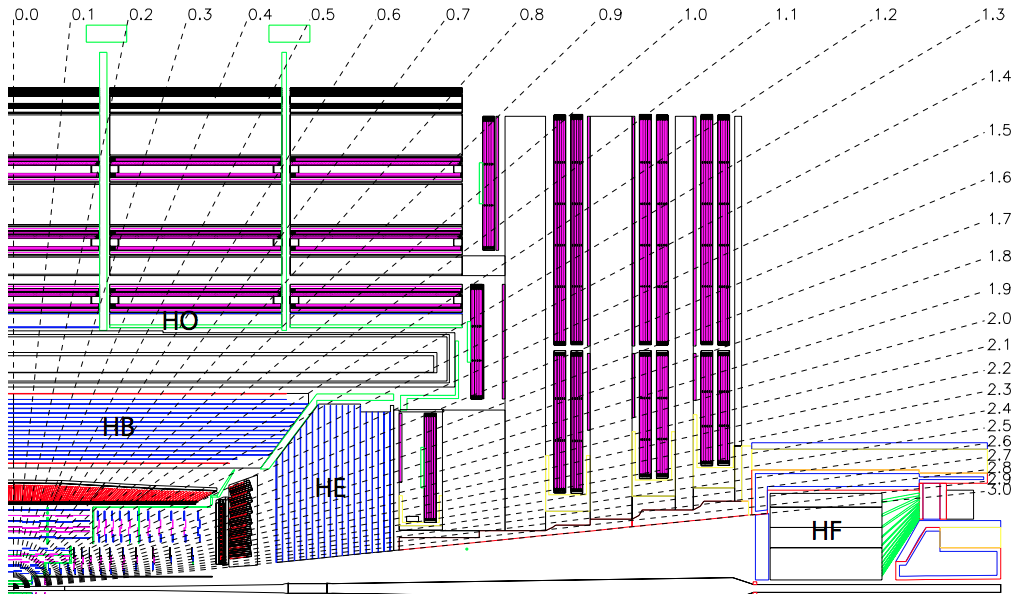
\includegraphics[width=\textwidth]{Figures/CMSHCAL}
	\caption[A geometrical quarter view of \acrshort{cms} HCAL, highlighting the Barrel (\acrshort{hb}), Endcap (\acrshort{he}), Forward (\acrshort{hf}) and Outer (\acrshort{ho}) subdetectors.]{A geometrical quarter view of \acrshort{cms} HCAL, highlighting the Barrel (\acrshort{hb}), Endcap (\acrshort{he}), Forward (\acrshort{hf}) and Outer (\acrshort{ho}) subdetectors. Figure taken from~\cite{CMSExperiment}.}
	\label{fig:CMSHCAL}
\end{figure}
% Inside the magnet need as much stopping power as possible - lots of short radiation length material, thin scintillating tiles (3.7mm)

As hadrons pass through the \acrshort{ecal} they leave only minimal deposits before entering the \acrshort{hcal}. 
When they continue through the dense absorption layers they interact and produce cascades of particles. 
These particle showers cause the plastic scintillator to emit blue-violet light which is passed by very small wavelength-shifting fibres as green light to the readout where the signal is amplified using hybrid photodiodes.
At small \abseta{} the stopping power of the \acrshort{hb} is not enough to fully contain the hadronic cascade so the \acrshort{ho} is used to catch the tails of the hadronic cascades improving the \ptmiss{} resolution of the detector.
The resolution of the \acrshort{hcal} is parametrised as 
\begin{equation}
	\frac{\sigma_{\mathrm{HCAL}}}{E} = \frac{S}{\sqrt{E}} + C,
\end{equation}
where $S$ is measured to be 0.85 and $C$ to be 0.07 in~\cite{CMS:HCALRES}.
This is similar to the expected resolution of hadronic cascades shown in Fig.~\ref{fig:CMSHCALRes} which are given in terms of reconstructed jet transverse energy.
% iterative cone methos with delta r = 0.5
Jet clustering will be discussed in Sec.~\ref{ssub:antikt}.

\begin{figure}[htpb]
	\centering
	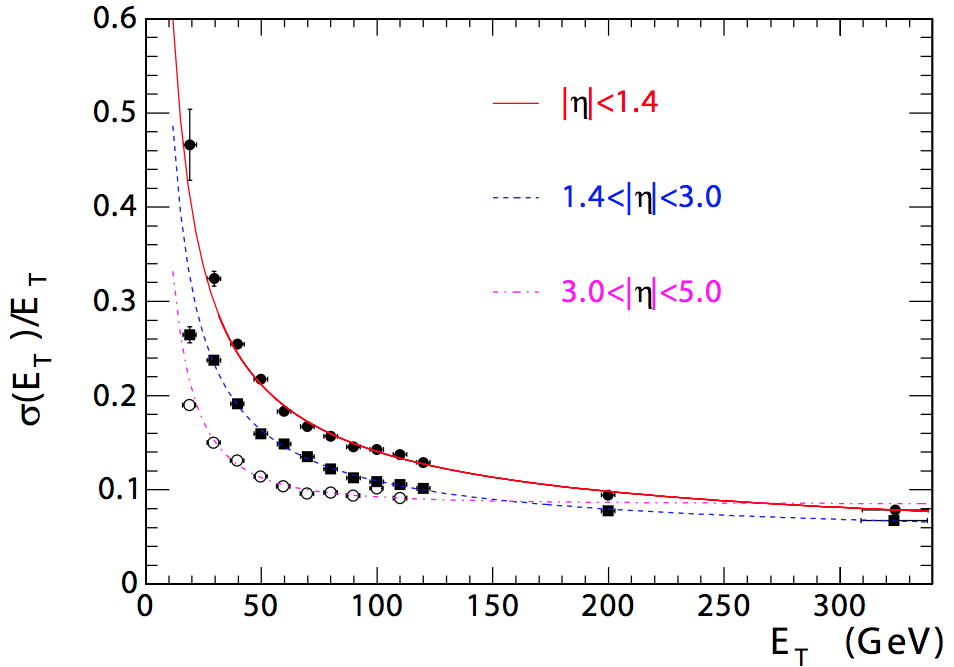
\includegraphics[width=0.7\textwidth]{Figures/CMSHCALRES}
	\caption[The transverse energy resolution of reconstructed jets in the \acrshort{cms} \acrshort{hcal}. It is split into the barrel jets ($\abseta<1.4$), endcap jets ($1.4<\abseta<3.0$) and forward jets ($3.0<\abseta<5.0$)]{The transverse energy resolution of reconstructed jets in the \acrshort{cms} \acrshort{hcal}. It is split into the barrel jets ($\abseta<1.4$), endcap jets ($1.4<\abseta<3.0$) and forward jets ($3.0<\abseta<5.0$) Figure taken from~\cite{CMSExperiment}.}
	\label{fig:CMSHCALRes}
\end{figure}

\subsection{Superconducting magnet}
\label{ssec:Magnet}
% http://iopscience.iop.org/article/10.1088/1748-0221/5/03/T03021/pdf

The solenoid at the heart of \acrshort{cms} is the largest superconducting magnet that has ever been built at 13\m{} long and 6\m{} in diameter.
It is composed from coils of a niobium-titanium alloy wire that are cooled to an operating temperature of 4.5\Kelvin{}. 
It operates at a field strength 3.8\Tesla{} reduced from a design operation field strength of 4\Tesla{} in order to maximise longevity.
The magnet and steel return yokes, which are used to contain the magnetic field, are the most massive components in \acrshort{cms} weighing approximately 12,000 tonnes.
The high field strength allows for very precise measurements of the curvature of charged tracks leading to precise measurements of the momenta of charged particles.

\subsection{Muon detectors}
\label{ssec:MuonChambers}

The muon chambers are the outermost set of detectors at \acrshort{cms}, interleaved with the steel return yoke of the superconducting solenoid.
There are three types of muon chamber present at \acrshort{cms}: resistive plate chambers (\acrshort{rpc}s), cathode strip chambers (\acrshort{csc}s) and drift tubes (\acrshort{dt}s).
The layout of the muon chambers is presented in Fig.~\ref{fig:CMSMuon}.
\begin{figure}[htpb]
	\centering
	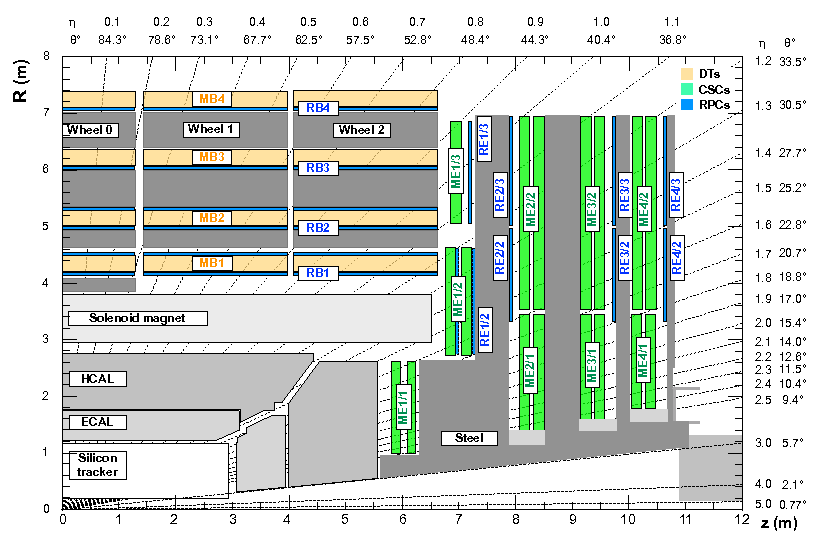
\includegraphics[width=0.95\textwidth]{Figures/CMSMUON}
	\caption[A geometrical one-quarter view of the \acrshort{cms} muon subsystems. The drift tube stations are indicated in yellow the cathode strip chambers in green and the resistive plate chambers in blue.]{A geometrical one-quarter view of the \acrshort{cms} muon subsystems. The drift tube stations are indicated in yellow the cathode strip chambers in green and the resistive plate chambers in blue. Figure taken from~\cite{CMSMuon}.}
	\label{fig:CMSMuon}
\end{figure}

The relatively low muon rates and uniform local magnetic field strengths in the barrel make \acrshort{dt} stations a good option for measuring muons in this phase space region covering up to $\abseta<1.2$.
Each cell is $13\times42\mmsq$ containing a gaseous mixture composed of 15\% $\mathrm{CO}_{2}$ and 85\% $\mathrm{Ar}$, with an anode central wire running the length of the cell.
As a charge is left in the cell, liberated electrons drift towards the central wire forming a signal.
The cells arranged into a set of four layers, each offset by half a cell-width to reduce non-sensitive detector regions, in what is know as a superlayer.
A set of three of the superlayers form a \acrshort{dt} muon station, where the outer two are aligned parallel to the beam line and the central one perpendicular.
This means the central superlayer can be used to calculate the $z$ co-ordinate and the outer two to measure the co-ordinates in $r,\,\phi$ space.
The \acrshort{dt} cells have a high spatial resolution but also a slow response time of up to 380\ns{}.
% drift time vs response time?
% Still very low occ with the high drift time (no mulithits) but large enough to be cost effective
% https://cds.cern.ch/record/1129810/files/jinst8_08_s08004.pdf

In the endcaps where the muon rates are higher, 540 \acrshort{csc}s are employed in the range $0.9<\abseta<2.4$. 
They have trapezoidal shapes to provide contiguous $\phi$ coverage in four disks in each endcap.
The \acrshort{csc}s have a quicker response time, a finer granularity and are less affected by variations in the magnetic field making them preferable to the \acrshort{dt}s.
Each \acrshort{csc} station consists of seven layers of cathode panels, each with strips milled running lengthwise at constant $\Delta\phi$ width, interleaved with six layers of azimuthally running anode wires.
The formation of six gas gaps are filled with 40\% $\mathrm{Ar}$, 50\% $\mathrm{CO}_{2}$ and 10\% $\mathrm{CF}_{4}$.
As a charged muon passes through the gas, electrons travel to the anode wires and ions to the cathode strips providing the co-ordinates in $r,\,\phi$ space.

Finally, 610 \acrshort{rpc}s are found in both the barrel (six layers) and endcaps (four layers) up to $\abseta<1.8$.
They are composed of gaseous parallel-plate detectors with two gas gaps filled with a mixture of 96.2\% $\mathrm{C}_{2}\mathrm{H}_{2}\mathrm{F}_{4}$, 3.5\% iso-$\mathrm{C}_{4}\mathrm{H}_{10}$ and 0.3\% $\mathrm{SF}_{4}$, separated by a common charge read-out strips.
The \acrshort{rpc}s have adequate spatial resolution, however they are complimentary to the \acrshort{dt}s and \acrshort{csc}s due to their very fast response time ($\approx2\ns$) which is much faster than the time it takes for the bunch crossing.
This makes the \acrshort{rpc}s ideal detectors for triggering muons, able to unambiguously identify the relevant bunch crossing a muon track is associated to.
Each component is discussed in more detail in~\cite{CMSExperiment,CMSMuon}.
% Double gap means each single gap operates at lower high voltage (gain) and higher detector efficiency.

Figure~\ref{fig:CMSMuonRes} shows the expected momentum resolution of the muons based on tracker information only, muon chamber information only and a combination of tracker and muon chamber information.
At low muon \pt{} the resolution is driven from the reconstruction of muons in the tracker, however as the \pt{} of the muon increases then the combination of information from the tracker and muon chambers results in improved resolution.

\begin{figure}[htpb]
	\centering
	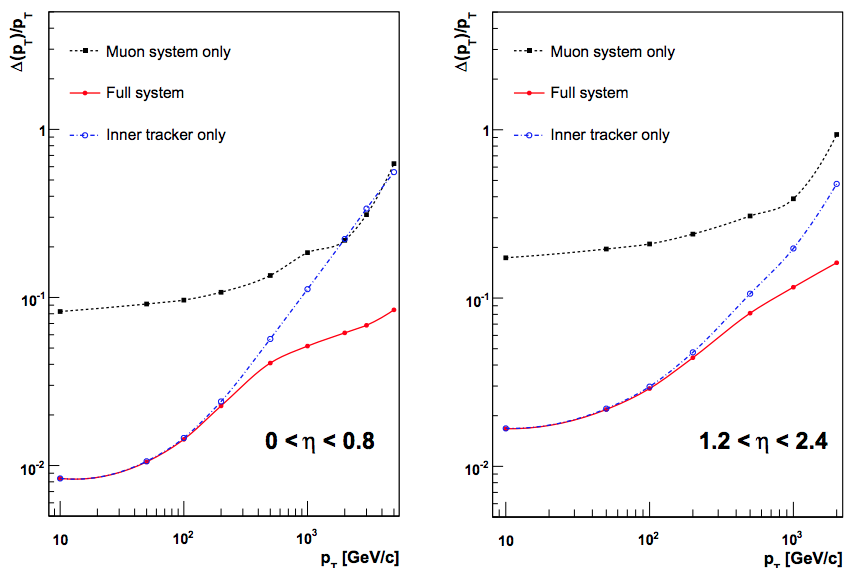
\includegraphics[width=0.85\textwidth]{Figures/CMSMUONRES}
	\caption[The muon \pt{} resolution as a function of \pt{} using the tracking only, muon subdetectors only or both.]{The muon \pt{} resolution as a function of \pt{} using the tracking only, muon subdetectors only or both. Figure taken from~\cite{CMSExperiment}.}
	\label{fig:CMSMuonRes}
\end{figure}
% Is this figure expected or data? I think expected...
% TODO GEMS?

\subsection{Triggers}
\label{ssec:Trig}

The \acrshort{cms} detector produces events at an approximate rate of 40\MHz{}. 
If each reconstructed event has a size of $\sim1\unit{MB}$, then data would be produced at a rate of 40~$\mathrm{TB}~\mathrm{s}^{-1}$. 
It is not feasible to fully reconstruct and store the full rate of data production so a method of data reduction, called triggering, is used. 
Triggering decides on an event-by-event basis whether a collision is likely to be highly-energetic and interesting, or just an elastic collision or low-energy QCD process. 
There are two types of triggering systems at \acrshort{cms}, the Level-1 hardware triggers (\acrshort{l1t}) and the High-Level software triggers (\acrshort{hlt}). 

The \acrshort{l1t} must decide within 3.2\us{} of an event occurring whether it should be rejected of tentatively accepted.
The schematic workflow of the \acrshort{l1t} is shown in Fig.~\ref{fig:CMSL1T}.
It uses only basic information from the detector known as \textit{trigger primitives} to make a decision.
These trigger primitives are formed from the calorimeter deposits and the hits in the muon detectors.
There are two trigger subsystems to the \acrshort{l1t}, the calorimeter trigger and the muon trigger.
These access the trigger primitives from different subdetectors and operate independently, with the exception of information passed from the calorimeter trigger to the muon trigger for the computation of muon isolation.
The outcome of both trigger components is then passed to the \acrshort{l1t} which makes the final decision on the event.
The \acrshort{l1t} reduces the event rate from 40\MHz{} to 100\unit{kHz}, which provides enough latency for the events to be fully reconstructed before being processed by the \acrshort{hlt}. 
Approximately 200 \acrshort{l1t} algorithms form the \textit{seeds} for the \acrshort{hlt}. 
The \acrshort{hlt} with access to the \acrshort{l1t} seeds and full event reconstruction, reduces the final physics production rate to 1\unit{kHz} and classifies the events into data sets with similar topologies, for example into sets containing a single isolated electron or sets that have high jet multiplicities.
\begin{figure}[htpb]
	\centering
	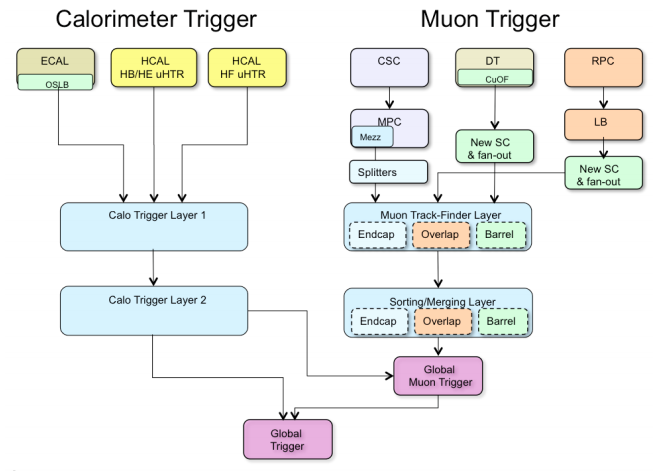
\includegraphics[width=0.85\textwidth]{Figures/CMSL1TUpgrade}
	\caption[A schematic representing the process flow of the \acrshort{l1t}. On the left is the calorimeter trigger and on the right the muon trigger which operate on independent trigger primitives. The final decision is taken by the global trigger using all information available.]{A schematic representing the process flow of the \acrshort{l1t}. On the left is the calorimeter trigger and on the right the muon trigger which operate on independent trigger primitives. The final decision is taken by the global trigger using all information available \cite{CMS:L1TUpgradeTDR}.}
	\label{fig:CMSL1T}
\end{figure}

\subsection{Computational power} % (fold)
\label{sub:computational_power}

The field in particle physics is unique in the way in which it shares data sets.
By considering just the samples stated in~\ref{tb:Gen}, there are conservatively one billion events leading to a total simulated data set size of $>1\unit{PB}$ in just this thesis alone.
As well as the simulated samples, the data sets produced by the \acrshort{lhc} must also be stored and together this is far too much for a single storage site to be viable or for every analysis to use a set of privately generated simulations and so the data sets must be shared.

Not only must data storage be shared across the collaboration, but also the processing power.
By taking the same number of events, it would take approximately two millenia to simulate the events (at one event per minute) and approximately eight months to run the analysis code for this thesis (at 20 events per second) on a single processing core.
Waiting almost two thousand years for data samples to be generated is clearly not feasible, therefore the data simulation and data processing need tens of thousands of cores. 

The \acrfull{wlcg} was created to share storage and processor resources.
The \acrshort{wlcg} is a tiered system with all raw data being stored at a central Tier-0 computing facility and subsequently distributed to Tier-1 and Tier-2 sites in the countries and institutes affiliated to \acrshort{cern}.
The complete set of raw data is stored at the \acrshort{cern} Tier-0 data centre, where the combined permanent archive stored on tape breached 200\unit{PB} on the 29th June 2017.
In terms of online storage the data centre at \acrshort{cern} holds 45\unit{PB} with a further 5.5\unit{PB} extension at the Wigner Research Centre for Physics in Budapest.
The 100,000 processor cores at the data centre deal with 1\unit{PB} of data every day.

The large Tier-1 facilities store a large fraction of the data and simulation sets so that there are multiple redundancies for every data set.
The 13 Tier-1 facilities are the main workhorses of the \acrshort{wlcg} performing large-scale reprocessing of the raw data sets and the generation of simulated events.

Tier-2 sites, of which there are 155, store data sets distributed to them from Tier-1 facilities and specific data sets that are useful for locally based analysis teams.
They provide a moderate number of processor cores for computational tasks, most generally for the production of simulated events.
The distributed nature of the file system allows for any person to access data sets from any site which has it stored and to use free computational power anywhere that is part of the \acrshort{wlcg}, increasing the overall computational efficiency.

% subsection computational_power (end)

\subsection{Data collection in 2016} % (fold)
\label{sub:data_collection_in_2016}

As already stated in Sec.~\ref{sec:lumi}, an integrated luminosity of \Lumi{} was collected by \acrshort{cms} in 2016.
To further classify the data used in this thesis, Tab.~\ref{tb:Data2016} shows the data collected with respect to the run period.
A run period refers to periods of similar data taking throughout the year.
Run period A is used for the commissioning of the detector.
Run periods often change after a short technical stop has occurred.
\begin{table}
	\centering
	\caption{The sets of single electron and single muon data collected during 2016 split into individual runs. A total luminosity of 35.9\fbinv{} of data was collected.}
	\label{tb:Data2016}
	\resizebox{\linewidth}{!}{%
	\begin{tabular}{llcc}
		\textbf{Channel}		&	\textbf{Data set}				& \textbf{Run ranges}	& \textbf{Luminosity (\fbinv{})} \\
		\hline
		SingleElectron(Muon)	 &	Run2016B-03Feb2017\_ver2-v2		& 272007--275376		&	5.79 \\
								 &	Run2016C-03Feb2017-v1			& 275657--276283		&	2.57 \\
								 &	Run2016D-03Feb2017-v1			& 276315--276811		&	4.25 \\
								 &	Run2016E-03Feb2017-v1			& 276831--277420		&	4.01 \\
								 &	Run2016F-03Feb2017-v1			& 277772--278808		&	3.10 \\
								 &	Run2016G-03Feb2017-v1			& 278820--280385		&	7.54 \\
								 &	Run2016G-03Feb2017-ver2(3)-v1	& 280919--284044		&	8.61 \\
		\hline
		Total integrated luminosity	 &	&  & 35.87 \\
	\end{tabular}%
	}
\end{table}

The initial data sets used in this thesis are classified as containing either a single electron or a single muon.
The \acrshort{hlt} trigger selections reduce the total number of events used from the initial data sets significantly, decreasing computational time.
In the \eJets{} channel the trigger requires there to be an electron with a $\pt>32\GeV$, a $\abseta<2.1$ and to pass a set of tight identification requirements (\eTrigger{}).
In the \muJets{} channel an isolated global muon or isolated tracker muon is required with a $\pt > 24\GeV$ and a $\abseta < 2.4$ (\muTrigger{}).

% subsection data_collection_in_2016 (end)

% Figure~\ref{CMSL1T} shows the 

% \begin{figure}[htpb]
% 	\centering
% 	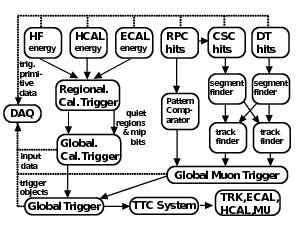
\includegraphics[width=0.7\textwidth]{Figures/CMSL1T}
% 	\caption[This needs a caption TODO Add ref in text]{This needs a caption TODO Add ref in text~\cite{CMSL1T}.}
% 	\label{fig:CMSL1T}
% \end{figure}

% \subsection{UpgradesToCome}
% \label{ssec:Upgrade}
% Track Trigger?
% \subsection{DataTaken}
% \label{ssec:DataTaken}

\newpage\null\thispagestyle{empty}
\chapter{Reconstructing the physics objects}
\label{ch:ObjectReconstruction}

Whether the components of an event are measured from a detector or simulated from a model, the deposits need to be reconstructed into physics objects. 
In CMS, the reconstruction of objects from the calorimeter energy deposits and charge deposits in the tracker and muon chambers is done by an algorithm called \textit{particle flow} (\PF{})~\cite{Event:PFlow}.
These collections of deposits are reconstructed into likely electrons, photons, muons, charged and neutral hadronic jets and missing \pt{} and are known as \textit{PF candidates}.
The \PF{} candidates undergo further, stricter identity cuts depending on the needs of the analysis, into high-purity collections of object candidates.
% The data object need to be corrected depending on the response of the subcomponents in the detector, \eg{} there should be no angular dependence on the energy of a particle.
% In addition, when comparing the simulation and data there may be differences present. The simulation needs to be corrected to match what is seen in the data.


\section{The particle flow algorithm}
\label{sec:PFlow}

The \PF{} algorithm is used to reconstruct objects to particle candidates, from the raw deposits in the event. 
The first step is to reconstruct the \textit{PF elements} to be used in the algorithm.
These elements are the charged particle tracks and vertices along with the calorimeter clusters and muon system hits.
Each final state particle can, in general, be matched to multiple \PF{} elements.
The combination of the correlated measurements, allows for the reconstruction and identification of particles.

\subsection{Particle flow elements} % (fold)
\label{sub:Particle_flow_elements}

Tracks are built in an iterative process.
Firstly, a track seed is generated for a triplet of hits in the pixel detector, with a few hits compatible with a charged-particle trajectory.
Next, additional hits are added, layer-by-layer, to the current track candidate based on the track seed trajectory, extrapolated via a Kalman filter~\cite{Event:KF}.
New track candidates are formed in this process when multiple hits match the extrapolation and track candidates with missing hits are also kept.
Once the outer tracker layer has been reached, possible duplicates are avoided by requiring each pair of track candidates to be composed of at least 50\% of unique hits.
If not, then the candidate with the most missing hits is dropped and if they are the same length then the one with the highest \chisq{} is dropped.
The final track fitting is then performed, using all associated track hits to determine the charged-particle properties (vertex, \pt{}, \etc{}).
Additional track quality cuts are imposed which include a minimum \pt{} cut of 0.9\GeV{}, the number of missing hits, the goodness-of-fit \chisq{} of the track fit and the distances to the beamline and a reconstructed primary vertex.
Once a track candidate is accepted its component hits are removed from the collection of tracker hits, and the process repeats, until no more track candidates can be found.
% Two fits actually formed. one PV to outer, second outer to PV.
% TODO iterate through different hit collections.

Primary vertices are reconstructed by clustering the reconstructed tracks according to the $z$-coordinate at the point of closest approach to the beam line.
An adaptive vertex fit is used on these sets of tracks to find the position of the vertex~\cite{Event:VertexFitting}.
The primary interaction vertex is defined as the primary vertex with the largest sum of $\pt^{2}$ from the objects associated to it.
A dedicated algorithm is used to identify secondary displaced vertices within the tracker volume, using the complete set of reconstructed tracks~\cite{Event:SecondaryVertex1,Event:SecondaryVertex2}.
These displaced vertices mainly originate from nuclear interactions with the tracker material or from conversion photons.

Muon track elements are identified using two different methods.
The first matches each track element present in the muon chambers to a track reconstructed in the inner tracking system and a track fit performed using a Kalman filter.
These track are called \textit{global} muon tracks.
The second method takes all tracks in the tracker and looks for compatible signatures in the calorimeters and in the muon chambers. 
If a compatible signature if found then the inner track is labelled as a \textit{tracker} muon track.

Calorimetric cluster candidates are constructed individually, but with a similar methodology, for the ECAL and HCAL. 
Initially, cluster seeds are created which are the local energy deposit in a cell which is maximal with respect to adjacent cells and above a seed energy threshold.
Next, bordering cells are added to the seed if they contain a deposit above a given cell energy threshold.
All thresholds can be found in~\cite{Event:PFlow}.
Calorimeter clusters not associated to an extrapolation of a track candidate are clear indicators of a neutral particle.
Care must be taken however, when a neutral-particle deposit overlaps a charged-particle deposit.
These are detected as an excess in cluster energy with respect to the sum of the \pt{} of the associated charged particles.
The method of obtaining an accurate calorimeter calibration in order to maximise the identification of the neutral clusters, while minimising the misreconstructed energy excesses and to get the correct energy scale for all neutral particles is also given in~\cite{Event:PFlow}.

% 4 in HCAL, 8 in ECAL.
%    X    X X X
%  X O X  X O X
%    X    X X X
% ?
% subsection Particle flow elements (end)

\subsection{Linking algorithm} % (fold)
\label{sub:linking_algorithm}

The next step in reconstructing a particle is to use a \textit{link algorithm} to connect all the requisite \PF{} elements together.
The probability for the link algorithm to connect two elements together depends on the granularity of the CMS subdetectors and the number of particles to resolve.
For a single particle, the probability to link all elements together depends predominantly on the volume of material traversed before the calorimeters due to nuclear interactions introducing trajectory kinks and secondary particles.

A link between the central track and calorimeter cluster is created if the extrapolation of the track candidate from the last hit position to a depth of one interaction length in the calorimeters is within a cluster candidate area. 
Neutral clusters in the ECAL are linked to electron brehmsstrahlung radiation if a tangential extrapolation (starting from tracker hit position) lies within the boundaries of a cluster candidate and the $\eta$ displacement between the cluster and original track candidate extrapolation is less than 0.05.
The brehmstrahlung photons have a high chance to form a pair of \textit{conversion electrons} (\electronp{}\electronm{}).
A conversion finder 
% TODOREF 
is used to find links between compatible track candidates originating from a photon conversion and if found is subsequently linked to the originating track candidate.
Links between ECAL, HCAL and preshower cluster candidates are formed if they are outside of tracker acceptance.
The cluster position in the more granular subdetector must lie within the cluster envelope of the coarser subdetector.
Charged particle tracks associated to a common secondary vertex are linked.
Finally, links can be created between a central track candidate and information from the muon detectors either as a global or a tracker muon track. 
All \PF{} elements linked together form a \textit{PF block}.

The \PF{} algorithm uses the \PF{} blocks as an input and performs reconstruction and identification in the following order.
Muon candidates are identified and reconstructed before removing the corresponding \PF{} elements form the \PF{} block.
Next, electrons are processed including brehmsstrahlung radiation concurrently with isolated photons and again associated \PF{} elements removed.
Finally, the remaining \PF{} elements are associated to charged hadrons, neutral hadrons and photons eminating from the fragmentation and hadronisation occurring within parton jets.
The reconstruction and identification of each \textit{PF object} is described in the following sections.
% subsection linking_algorithm (end)

% subsection pf_isolation (end)

\subsection{PF muons} % (fold)
\label{sub:pf_muons}

\PF{} muons are identified from the global and tracker muon track properties.
First, isolation requirements are imposed on the global muon tracks.
Isolation is a measure of the activity of the event around the object of interest.
In this case, additional tracks and calorimeter deposits are taken within a cone of 
\begin{equation}
	\Delta R=\sqrt{\smash[b]{(\Delta\eta)^2+(\Delta\phi)^2}} < 0.3,
\end{equation}
and if 
\begin{equation*}
	\sum\pt^{\text{track}}+\sum\ET^{\text{calo}} < 0.1\times\pt^{\text{muon}},
\end{equation*}
then no further selection is required as hadrons misidentified as muons are rejected adequately.
Above this value, charged hadrons are susceptible to be misreconstructed as muons, due to \textit{punch-through} from the back of the HCAL.
% These mean that charged tracks will be taken away from HCAL deposit leaving spurious neutral particles left.
% In addition if a muon stops in the HCAL then it is reconstrcted as charged hadron and saps adjacent neutral deposits.
In this regime, the global muons must pass a tight-muon identification criteria described in Sec.~\ref{sec:mu} and either at least three matching hits found in the muon chambers or the calorimeter deposit is compatible with the muon hypothesis.
If the muon does not pass the tight-muon ID due to a poor inner or global fit, then it is retained if the tracker muon fit is of high quality and the calorimeter deposit is compatible with the muon hypothesis.

For muons with $\pt<200\GeV$, the muon track resolution is better for tracker muons than for global muons and so the tracker muon track is used to determine the muon properties.
Otherwise they are taken from the track fit with the minimum \chisq{}.
% tracker, tracker + muon chamber 1, global, global minus high occ muon chambers.
% subsection pf_muons (end)

\subsection{\PF{} electrons and photons} % (fold)
\label{sub:pf_electrons_and_photons}

Due to the similarity in the basic properties of electrons and isolated photons (electrons emit brehmstrahlung photons and photons convert to \electronp{}\electronm{} pairs), the \PF{} algorithm reconstructs isolated \PF{} photons and \PF{} electrons simultaneously.
\PF electrons are seeded from a cluster candidate linked to a \GSF{} (Gaussian sum filter) track~\cite{Event:GSF}, given that it is not additionally linked to more than three other tracks.
Isolated \PF{} photons are seeded from clusters $>10\GeV$ with no link to a \GSF{} track.

\GSF{} tracks are based on a combination of two different methods of track reconstruction.
The first is the \textit{ECAL-based} method, which extrapolates to the inner track hits depending on the ECAL cluster energy and position.
To seed the ECAL-based track all clusters of $\ET>4\GeV$ are used with the assumption that they are produced by either an electron or positron.
A large proportion of the energy of the electron or positron is lost to bremhstrahlung and so the performance of the method depends strongly on the ability to collect all the associated energy depositions and without depositions from other particles.
To collect the energy, the cluster is extended in $\phi$ around the electron direction to account for the bending in the magnetic field.
The group of clusters is known as a \textit{supercluster}.
The ECAL-based track seeds suffer at low-\pt{} due to the large bending in the magnetic field and in jets due to the non-isolated environment.
The second is the \textit{tracker-based} method and recovers electron tracks missed by the ECAL-based approach.
It starts from the iterative-based track candidates with a $\pt>2\GeV$, with more specific requirements of the number of missing hits and the \chisq{} of the track fit.
A \GSF{} fit (which is reduced) is used on the track hits as it is more suitable to electron fitting than a Kalman filter.
A final cut on a boosted-decision-tree that combines the discriminating power of a number of distributions, \eg{} the \chisq{} of the \GSF{} fit, the distance between the extrapolated track and the nearest cluster and the energy lost along the \GSF{} track, is used to select tracker-based track seeds.
The track seeds obtained by the two methods are combined together and a final full \GSF{} fit processed.

\PF{} electrons are required to satisfy additional identification criteria on both the track seed and cluster properties.
These criteria include the track fit \chisq{}, the ratio of energy in the HCAL to the ECAL and the number of hits.
A full set of parameters is given in~\cite{Event:PFlow}.
\PF{} photons are selected depending on compatibility with the photon hypothesis of the isolation with respect to \GSF{} tracks and clusters, the shower shape and the ECAL to HCAL energy ratio.

% non-isolated environment: SC affected by non electron deposits. track matchiong therefore affected. Lots of misreconstruction.
% Brehmstrahlung occurs when charged particle passes through material and is accelerated by protons.
% what specific requirements
% azimuthal bending
% GSF fit describes energy loss in each layer.

% subsection pf_electrons_and_photons (end)

\subsection{PF jets} % (fold)
\label{sub:pf_jets}

Once the electrons, isolated photons and muons have been reconstructed and removed from the \PF{} blocks, the remaining particles must be from neutral hadrons, charged hadrons or non-isolated photons formed from the hadronisation of the final state.
Hadronic jets are composed of these hadrons and photons, where the photon content deposits primarily in the ECAL, the neutral hadron content in the HCAL and charged hadron content in both calorimeters.

All calorimetric \PF{} elements that are not linked to a tracking element are considered to be either neutral hadrons or photons.
Within the tracking acceptance the charged and neutral hadrons can be identified separately and as the neutral hadrons only leave $\approx3\%$ of the jet energy in the ECAL, the ECAL deposits are considered to originate solely from photons and the HCAL deposits from neutral hadrons.
Outside the tracking acceptance however, there is no way to separate charged hadrons from neutral hadrons.
As the charged hadrons also leave deposits in the ECAL, it is not possible to assign the deposits to photons alone.
Now the links between ECAL deposits and HCAL deposits become important. 
ECAL deposits not linked to HCAL are considered to be photons, while linked deposits are considered to arise from a neutral or charged hadron.

Once the neutral hadrons and non-isolated photons have been identified and removed, there are only calorimeter elements linked to one or more track elements remaining.
These make up the charged hadrons.
\PF{} jets are created by using the anti-\kt{} jet clustering algorithm on particles reconstructed from \PF{} algorithm, with a distance parameter $\Delta R<0.4$.

\subsubsection{Anti-\kt{} jet clustering algorithm} % (fold)
\label{ssub:antikt}

The charged and neutral hadron deposits are clustered using the anti-\kt{} jet clustering algorithm~\cite{Event:antikt}.
% This algorithm is infrared and collinear safe.
It is an extension to the Cambridge/Aachen and \kt{} jet clustering algorithms.
These algorithms work by calculating the distance between two entities, either particles or proto-jets $d_{ij}$ and the distance between an entity and the beam line, $d_{iB}$.
If the smallest distance is between two entities then they are recombined into a new proto-jet, whereas if $d_{iB}$ is smaller, then $i$ is called a jet and removed from the list of entities.
All distances are then recalculated and the clustering repeated until no entities remain.
The maximum cone size is given by the double of the radius parameter, $R$.
The differences between the anti-\kt{} algorithm occur in the definition of the distance parameters
\begin{equation}
	d_{ij} = \mathrm{min}(k_{Ti}^{2p},k_{Tj}^{2p})\frac{\Delta^{2}_{ij}}{R^{2}}
\end{equation}
and
\begin{equation}
	d_{iB} = k_{Ti}^{2p}.
\end{equation}
The parameter $p$ gives the strength of the relative contributions to $d_{ij}$ and $d_{iB}$ from the hardness of the entity and the angular separation.
The angular separation is defined as 
\begin{equation*}
	\Delta_{ij}=\sqrt{(y_i-y_j)^2+(\phi_i-\phi_j)^2}.	
\end{equation*}
For $p=+1$ the \kt{} algorithm is recovered and the Cambridge/Aachen algorithm when $p=0$.
The anti-\kt{} algorithm uses $p=-1$ which means that precedence is given to the hardness of the entities, \eg{} a soft particle is much more likely to cluster to a hard particle than another soft one.
This leads to perfectly conical jets if no two initial hard particles are within $2R$ of each other.
If there are two hard particles within $R<\Delta_{12}<2R$ but $k_{T1}^{2}>>k_{T2}^{2}$ then the hardest jet will be conical and the softer a cone missing the overlap.
If $k_{T1}^{2}\sim k_{T2}^{2}$ then the jet boundary will lie between the two jet axes.
For closely spaced hard particles within $\Delta_{12}<R$, clustering will occur, but for $k_{T1}^{2}\sim k_{T2}^{2}$ the shape becomes a union of the cones of both constituent hard particles as well as the cone centred on the final jet.
This means that the anti-\kt{} algorithm is resilient against soft radiation but adaptive to hard emission.
An example anti-\kt{} jet clustering is shown in Fig.~\ref{fig:antikt}.
\begin{figure}[htpb]
	\centering
	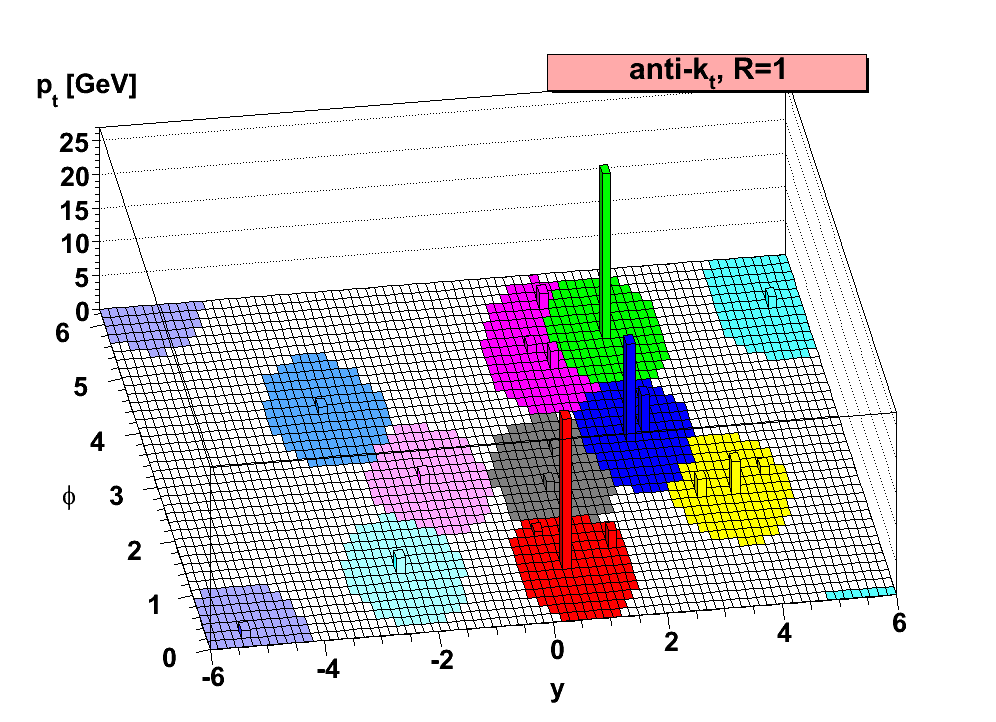
\includegraphics[width=0.8\textwidth]{/Users/db0268/Desktop/Thesis/Figures/Event_antikt.png}
	\caption[An example of clustering using the anti-\kt{} algorithm. Soft particles are preferentially clustered around high-\pt{} seeds forming conical jets. The jet boundary is defined by the respective hardness between neighbouring jets.]{An example of clustering using the anti-\kt{} algorithm. Soft particles are preferentially clustered around high-\pt{} seeds forming conical jets. The jet boundary is defined by the respective hardness between neighbouring jets. Figure taken from~\cite{Event:antikt}.}
	\label{fig:antikt}
\end{figure}

As the particle flow algorithm attempts to reconstruct every individual particle in an event, before the jet clustering, it is possible to assign charged hadrons to either a high-\pt{} interaction vertex or an additional interaction vertex.
If definitely matched to a pileup vertex then the associated jet constituents are removed.
This is known as \textit{charged hadron subtraction}.
If there is no clear association then the charged hadrons remain in the jet.
Pileup subtraction is discussed further in Sec.~\ref{sub:jet_energy_corrections}.
% about 50% of the offset energy is charged hadrons.
% photon content ~25% of jet, neutral hadrons only leave 3% in ECAL
% subsubsection subsection_name (end)

\subsubsection{Identification of \bquark{} quark jets} % (fold)
\label{ssub:bqj}

The properties of a jet arising from a \bquark{} quark are different enough to those of a jet formed from a \uquark{}\dquark{}\squark{} quark or gluon that it is possible to discriminate between them.
The ability to do this is very important for many analyses, especially those involving top quark physics because it reduces the impact from background processes considerably.
The crucial aspect of this discrimination arises from the formation of \bquark{} hadrons from the \bquark{} parton, which have a longer lifetime and typically travel a few millimetres in the detector before decaying.
Figure~\ref{fig:secvert} shows an illustration of a heavy-flavour jet associated to a secondary vertex.
\begin{figure}[htpb]
	\centering
	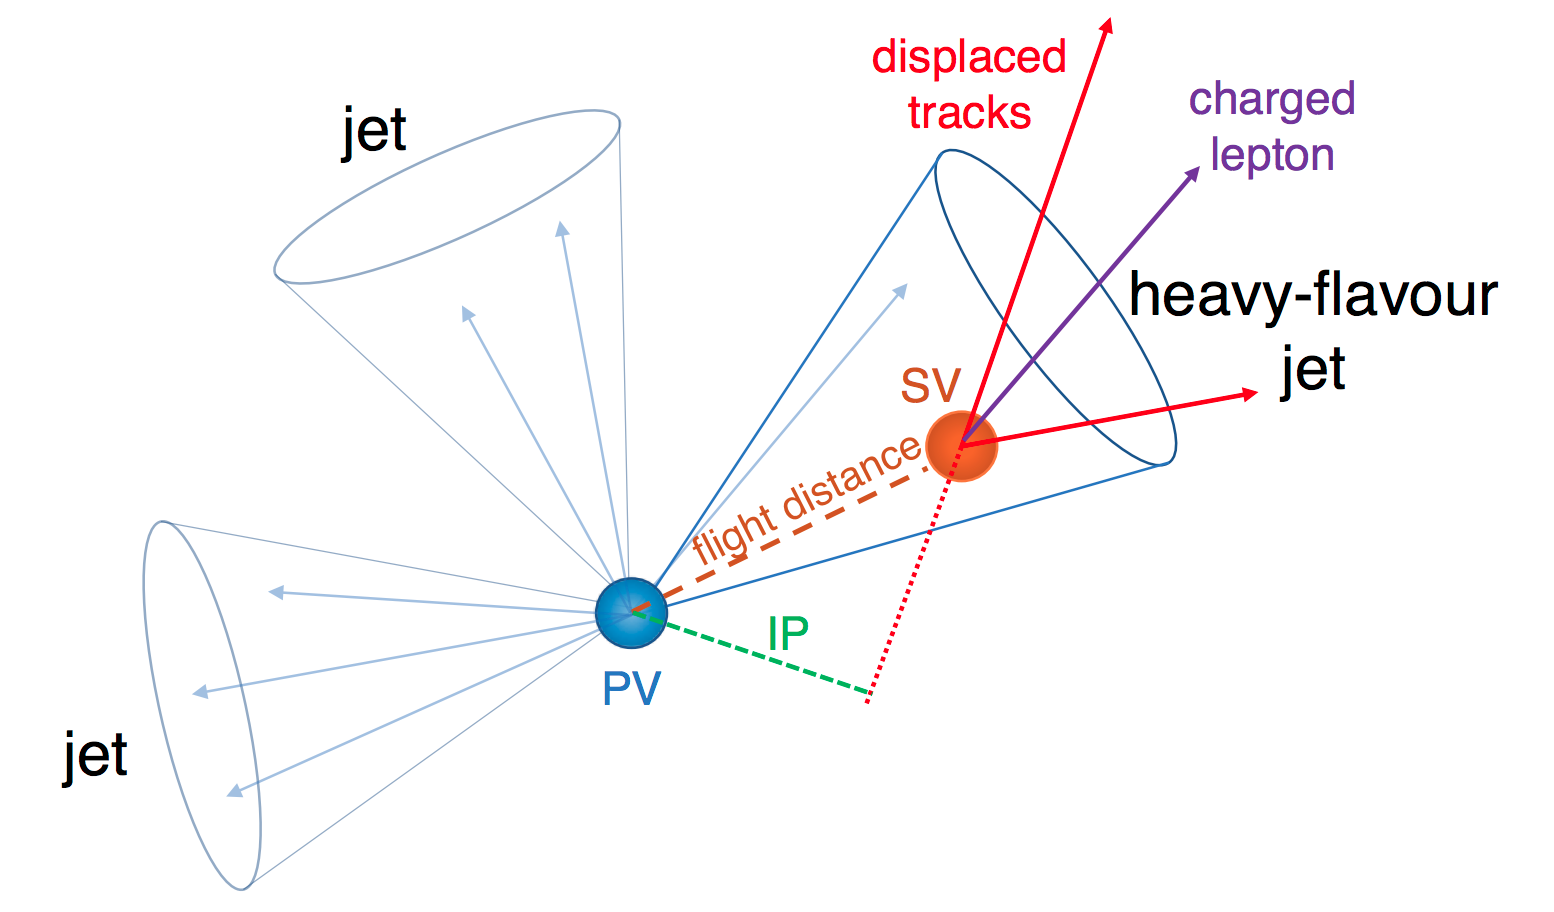
\includegraphics[width=0.8\textwidth]{/Users/db0268/Desktop/Thesis/Figures/Event_BTag.png}
	\caption[An illustration of a jet from a heavy flavour quark. A hadron is formed with a lifetime of $\sim1-1.5\ps$ which decays at a displaced secondary vertex (SV) with respect to the primary interaction vertex (PV) and hence has a large impact parameter (IP).]{An illustration of a jet from a heavy flavour quark. A hadron is formed with a lifetime of $\sim1-1.5\ps$ which decays at a displaced secondary vertex (SV) with respect to the primary interaction vertex (PV) and hence has a large impact parameter (IP). Figure taken from~\cite{Event:BTV}}
	\label{fig:secvert}
\end{figure}
The discriminating variables include the displaced tracks from the secondary vertex, the impact parameter, the increased fragmentation due to the higher initiating mass which can lead to both increased \pt{} measurements with respect to the jet axis and a greater proportion of charged leptons in the jet constituents.

The \textit{combined secondary vertex} algorithm (\CSV)~\cite{Event:BTV} takes this information and assigns a discriminator value between 0 and 1.
The closer the discriminating value to 1 the more likely the jet is to be a \bquark{} jet.
The flavour composition of jets with respect to \CSV{} discriminant is shown in Fig.~\ref{fig:csv}, using a basic event selection applied to a \ttbar{} simulation.
It is immediately clear that applying a requirement for two high \CSV{} values, enhances the number of events with two jets emanating from \bquark{} quarks and thus the number of signal \ttbar{} events with respect to background processes.
\begin{figure}[htpb!]
	\centering
	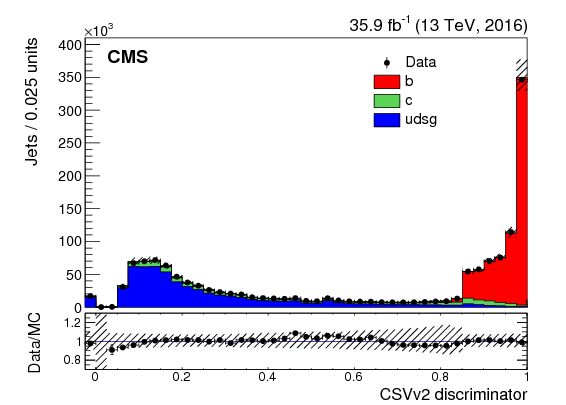
\includegraphics[width=0.8\textwidth]{/Users/db0268/Desktop/Thesis/Figures/Event_CSVv2.png}
	\caption[The flavour composition of jets from a \ttbar{} model simulation. A simple event selection is performed requiring an isolated lepton, four jets with $\pt>30\GeV$ of which two are required to have $\CSV>0.8484$.]{The flavour composition of jets from a \ttbar{} model simulation. A simple event selection is performed requiring an isolated lepton, four jets with $\pt>30\GeV$ of which two are required to have $\CSV>0.8484$. Figure taken from~\cite{Event:BTV}.}
	\label{fig:csv}
\end{figure}

% By applying a requirement that two jets in an event must have a $\CSV>0.8484$, the selection efficinecy for \ttbar{} events in this thesis increases from to 61\% to 92\%.

% \begin{figure}[htpb]
% 	\centering
% 	\includegraphics[width=0.49\textwidth]{/Users/db0268/Mount/SoolinScratch/DPS/DPSTestingGround/DailyPythonScripts/plots/control_plots/Nominal/Variables/Ref_selection_NoBSelection/COMBINED_CSV_2orMoreBtags_with_ratio}
% 	\includegraphics[width=0.49\textwidth]{/Users/db0268/Mount/SoolinScratch/DPS/DPSTestingGround/DailyPythonScripts/plots/control_plots/Nominal/Variables/Ref_selection/COMBINED_CSV_2orMoreBtags_with_ratio}
% 	\caption[Change to quark content type for ttbar only? TODO]{Change to quark content type for ttbar only? TODO}
% 	\label{fig:csvtmp}
% \end{figure}
% subsection pf_jets (end)

\subsection{PF missing transverse momentum} % (fold)
\label{sub:pf_ptmiss}

Conservation of momentum states that the sum of all transverse momentum is zero.
The presence of a momentum imbalance \ptmissvec{}, implies an undetectable particle in the event, \eg{} a neutrino.
In terms of particle flow, \ptmissvec{} is given by the negative vector sum of all the present particle flow objects
\begin{equation*}
	\ptmissvec = - \sum_{i}^{\mathrm{PF\,objects}} \vec{p}_{\mathrm{T}}^{\,\,i}.
\end{equation*}
More generally, the magnitude of this missing momentum is used \ptmiss{}. 
In most events \ptmiss{} is small, however there is a small probability that it is reconstructed to be artificially large.
The cause of this is most often the misreconstruction or misidentification of a high-\pt{} muon.
If an event has a large \ptmiss{} then the \PF{} algorithm applies a post processing step.
The first issue investigated are genuine muons from the cosmic ray muon background coincident with a bunch crossing.
They are recognised as such if their trajectory is more than 1\cm{} away from the beam line and removed from the particle flow collection is the \ptmiss{} is reduced by at least one half.
The second issue relates to bad reconstruction of the momentum of the muon, notified by significant differences in the global and tracker muon \pt{} estimates.
The bad reconstruction can be caused by interactions in the steel return yoke, in-flight decays and incorrectly assigned hits in the inner tracker.
If the \ptmiss{} is reduced by at least one half when recalculating with respect to the different muon \pt{} estimates then the muon estimate with the lowest \ptmiss{} is taken.
The third issue comes from the misidentification of a charged hadron punching through into the muon chambers.
A muon is reconstructed together with an energetic neutral hadron from the calorimeter deposits.
A similar issue is that of an overlapping muon and neutral hadron deposit being misreconstructed as a charged hadron deposit.
The particles are substituted with each other respectively if the \ptmiss{} is reduced by at least one half.

The \ptmiss{} is corrected accordingly when jet energy corrections (JEC), explained in Sec.~\ref{sub:jet_energy_corrections}, are applied to the PF jets.
\begin{equation*}
		\ptmissvec = - \sum_{i}^{\mathrm{PF\,objects}}{\vec{p}_{\mathrm{T}}^{\,\,i}} - \sum_{j}^{\mathrm{PF\,jets}}({\vec{p}_{\mathrm{T}}^{\,\,j,\,\mathrm{corr}}-\vec{p}_{\mathrm{T}}^{\,\,j})}.
\end{equation*}
% subsection pf_ptmiss (end)



\subsection{PF isolation} % (fold)
\label{sub:pf_isolation}

The requirement of leptons to be isolated has already been used in the reconstruction of the \PF{} objects.
Often, more stringent isolation selections are required and so the \textit{PF relative isolation} \Irel{} is employed.
It is defined as the ratio of the additional \pt{} within a cone of set distance around the lepton to the \pt{} carried by the lepton.
The additional \pt{} includes all charged and neutral hadrons as well as photons present within the cone.
\begin{equation}
\label{eq:pfiso}
	\Irel^{\ell} = \frac{\sum\pt^{\mathrm{charged}} + \sum\pt^{\mathrm{neutral}} + \sum\pt^{\gamma}}{\LPT}.
\end{equation}
In addition, contributions from additional interactions can be taken into account.
Charged particles from these extra interactions are not associated to the primary vertex and are removed.
Direct removal is not possible for neutral particles produced by the pileup.
One possible correction for this neutral pileup is the $\Delta\beta$ correction.
This uses the ratio of charged hadrons to neutral hadrons and photons in inelastic collisions to estimate the contribution of non-charged pileup from charged pileup.
The correction $\Delta\beta$ is set as 0.5.
The relative isolation then becomes
\begin{equation}
\label{eq:pfiso}
	\Irel^{\ell} = \frac{\sum\pt^{\mathrm{charged}} + \max(0, \sum\pt^{\mathrm{neutral}} + \sum\pt^{\gamma} - \Delta\beta\sum\limits^{}_{\mathrm{pileup}}\pt^{\mathrm{charged}})}{\LPT}.
\end{equation}

\section{Analysis object selection}
\label{sec:analysis_objects}

While the \PF{} algorithm is good at resolving particles, it is sometimes necessary to impose stricter identification criteria.
By increasing the probability that an analysis object is correctly reconstructed, the selection efficiency for that object decreases correspondingly.
Where the statistical uncertainty is not an issue or where an analysis requires a high object purity \textit{tighter} cuts tend to be used.
This is the case for \ttbar{} events produced at the LHC, having both a high cross section and large data set sizes.
In the following the identification criteria for all the objects used in this thesis will be detailed.

\subsection{Electron objects}
\label{sub:el}

As stated in Sec.~\ref{sub:data_collection_in_2016}, events that pass the \eTrigger{} trigger are selected as the basis of the \eJets{} channel in this thesis.
A harder \LPT{} cut is chosen at $\LPT>34\GeV$ to operate in a region optimal with respect to the trigger efficiency.
The $\LETA{}<2.1$ cut is maintained, however electrons falling into the gap between the barrel and endcap ($1.4442<\LETA<1.566$) are discarded.
The signal electron object must pass a set of strict identification requirements (\textit{tight} ID).
An additional collection of veto electrons are selected using a lower $\LPT>15\GeV$ and a looser set of identification criteria (\textit{veto} ID).
% The collections of objects are discussed in the event selection in Section TODO.
% ie outside trigger turn!

\subsubsection{Electron identification}
\label{ssub:el}
Further identification requirements are placed on the \PF{} electrons to be used as analysis objects. 
The additional requirements are combined into an electron identification which provides more discrimination for isolated prompt signal electrons against hadronic jets, fake electrons and other background sources of electrons.
The electron identification is provided by the E/gamma \textit{physics object group} (POG) for different working points in the barrel and endcap regions of the detector.
The tight and veto IDs are shown in Tab.~\ref{tb:elID}. 
The shower shape variable $\sigma_{i\eta i\eta}$ is the root-mean-square of the position of the energy deposited in a $5\times5$ lattice centred in the seed crystal.
An electromagnetic shower will be much more confined than a hadronic shower and therefore have a lower value of $\sigma_{i\eta i\eta}$.
The absolute differences in $\eta$ and $\phi$ between the supercluster position and the track direction at the primary vertex extrapolated to the ECAL assuming no brehmstrahlung radiation is given by $|\Delta \eta_{in}|$ and $|\Delta \phi_{in}|$.
Additional particles present in hadronisation processes bias the position of the supercluster due to the increased bending in low-\pt{} radiations.
The ratio of the hadronic energy to the electromagnetic energy $\sfrac{H}{E}$ is smaller for deposits from electrons than from hadrons.
A tighter requirement on the \PF{} isolation with effective area correction, using a cone size of $\Delta R < 0.3$, is included.
The effective area method subtracts the product of the effective area of the cone and the offset energy density, visited in Sec.~\ref{sub:jet_energy_corrections}.
It is more suitable than the $\Delta\beta$ correction due to being insensitive to the electron radiations.
The variable $|\sfrac{1}{E}-\sfrac{1}{p}|$ is proportional to the radius of curvature of the electron track and gives additional discrimination against electrons from conversion photons.
The missing inner hits requirement provides a stricter track quality acceptance than present in the \PF algorithm.
A selected electron is not allowed to originate from an identified conversion photon.
In addition to the electron identification, the electron must originate close to the primary vertex $d_{0}$ and close to the beam line $d_{z}$.
\begin{table}[h!]
    \centering
    \caption{The identification criteria for signal electrons (tight) and veto electrons (veto). The critera are split into the barrel and endcap regions at $\abs{\eta_{SC}}=1.479$} 
    \label{tb:elID}
    \begin{tabular}{lccccc}
                            &  & \multicolumn{2}{c}{\textbf{Tight}}    & \multicolumn{2}{c}{\textbf{Veto}}  \\
            \textbf{ID variable}    &  & \textbf{Barrel} & \textbf{Endcap}     & \textbf{Barrel} & \textbf{Endcap} \\
            \hline
            full $5\times5 \sigma_{i\eta i\eta}$    & $ < $ & 0.00998 & 0.0292  & 0.0115  & 0.037         \\
            $|\Delta \eta_{in}|$                    & $ < $ & 0.00308 & 0.00605 & 0.00749 & 0.00895       \\
            $|\Delta \phi_{in}|$                    & $ < $ & 0.0816  & 0.0394  & 0.228   & 0.213         \\
            $\frac{H}{E}$                           & $ < $ & 0.0414  & 0.0641  & 0.356   & 0.211         \\
            PF \Irel with EA correction        & $ < $ & 0.0588  & 0.0571  & 0.175   & 0.159         \\
            $|\frac{1}{E}-\frac{1}{p}|$             & $ < $ & 0.0129  & 0.0129  & 0.299   & 0.15          \\
            Missing Inner Hits                      & $ <= $& 1       & 1       & 2       & 3             \\
            Conversion Veto                         &       & Y       & Y       & Y       & Y             \\
            \\
            \textbf{Additional to ID} & & & & & \\   
            \hline
            $d_{0}\,(\cm\,)$                        & $ < $ & 0.05    & 0.10    & 0.05    & 0.10          \\
            $d_{z}\,(\cm\,)$                        & $ < $ & 0.10    & 0.20    & 0.10    & 0.20          \\
    \end{tabular} \\
\end{table}

% $|\Delta \eta_{in}|$ and $|\Delta \phi_{in}|$ are the absolute $\eta$ and $\phi$ differences between the SC position of the electron and the track direction at the primary vertex extrapolated to the ECAL assuming no Brehmstrahlung has occured. These cuts are used as the SC position can be biased by additional particles associated with hadron and conversion backgrounds. TODO(heavier particles bend more? more emission?) When an electron emits Brehmstrahlung radiation the $\phi$ distribution gets smeared TODO(so cuts are much hugher for phi than eta). 

\subsection{Muon objects}
\label{sec:mu}

Signal analysis muons must have a $\LPT>26\GeV$ cut, similarly imposed from the efficient operation region of the \muTrigger{} trigger selection and must pass tight ID requirements.
Veto analysis muons have a $\LPT>15\GeV$, aligned with that in the \eJets{} channel and must pass a \textit{loose} muon ID.

\subsubsection{Muon identification}
Analysis muons are selected from the \PF{} muons by applying a muon identification in an identical manner to the analysis electrons.
The criteria of the identity are listed in Tab.~\ref{tb:muID} and are supplied by the muon POG.
For signal muons, hits are required along the entire path of the muon from the silicon pixel detector to the muon chambers.
A good \chisndf{} of the track fit is also required.
Constraints are placed with respect to the primary vertex and beam line as with the electron identification.
Finally, a more stringent cut on the \PF{} \Irel{} with $\Delta\beta$ correction using a cone size of $\Delta R < 0.4$ is required.
\begin{table}[h!]
    \centering
    \caption{The identification criteria for signal muons (tight) and veto muons (loose).}
    \label{tb:muID}
    \begin{tabular}{lccc}
            \textbf{ID variable}      			&		&  \textbf{Tight}    & \textbf{Loose}  \\
            \hline
            is \PF{} muon 				&		&	Y				 &	Y \\			
            is global or tracker muon 	&		&	Y				 &	Y \\	
            Pixel hits 					&	$>$	&	0				 &	\NA{} \\	
            Tracker layer hits 			&	$>$	&	5				 &	\NA{} \\	
            Muon stations hit           &   $>$ &   2                &  \NA{} \\    
            Muon chambers hit           &   $>$ &   1                &  \NA{} \\    
            \chisndf{}                  &   $<$ &   10               &  \NA{} \\
            $d_0\,(\cm\,)$ 					&	$<$	&	0.2		 &	\NA{} \\
            $d_z\,(\cm\,)$ 					&	$<$	&	0.5		 &	\NA{} \\
            \\
            \textbf{Additional to ID} & & & \\   
            \hline
            PF \Irel{} with $\Delta\beta$ correction   & $ < $ & 0.15  & 0.25  \\
    \end{tabular} \\
\end{table}




\subsection{Jet Objects}
\label{sec:jet}

On top of the charged hadron subtraction in the \PF{} algorithm, analysis jets are required to have $\pt>30\GeV$, $\abseta<2.4$ and pass a loose ID supplied by the Jet/MET POG, shown in Tab.~\ref{tb:jetID}.
To ensure a jet is not additionally classified as a lepton it must have a minimum distance to the nearest lepton $\Delta R > 0.4$.
If the jet is close to a lepton then it is assumed to have originated from that lepton and is consequently removed from the jet collection. 
A jet is additionally classified as a \bquark{} jet, if it also passes the medium working point of the \CSV{} algorithm.
\begin{table}[h!]
    \centering
    \caption{The identification criteria for signal jets.}
    \label{tb:jetID}
    \begin{tabular}{lcc}
            \textbf{Cut}      			&		    & \textbf{Loose}  \\
            \hline
            Neutral hadron fraction 			& $<$ &	0.99 \\			
            Charged hadron fraction           	& $>$ &	0 \\		   
            Neutral electromagnetic fraction 	& $<$ &	0.99 \\		
            Charged electromagnetic fraction    & $<$ & 0.99 \\
            Number of constituents 				& $>$ &	1 \\		
			Number of charged constituents      & $>$ &	0 \\		
            Muon fraction 						&  	  & \NA{} \\		
    \end{tabular} \\
\end{table}




% \itemize{
% 	\item TODO: TRACK FIT - ITERATE THHROUGH DIFF TYPES OF SEEDS
% 	\item TODO: KALMAN FILTER REF
% 	\item TODO: CONVERSION FINDER REF
% 	\item TODO: TIGHT MUON ID AT PF LEVEL
% }

\chapter{Analysis formation, event selection and corrections}
\label{ch:analysis}

With the complete reconstruction of events in both data and simulation it is possible to begin forming an analysis.
Several variables are defined to be measured and an appropriate event selection must be formed, dependent on the event topology that is being investigated.
Corrections still need to be applied to the analysis objects to resolve any remaining differences between data and simulation.
Before the event selection, data objects are corrected depending on the response of the subcomponents in the detector, \eg{} there should be no angular dependence on the energy of a particle.
Then the simulation is then corrected to match what is observed in the data, \eg{} due to differences in the efficiencies of the various reconstruction algorithms applied.
Once the \ttbar{} yields have been calculated after all corrections are applied, then the cross sections can be measured.

\section{Kinematic event variables and the event selection}
\label{sec:var}
As stated in Sec.~\ref{sub:top_quark_cross_section_measurements}, this thesis measures seven event variables which are \NJET{}, \HT{}, \ST{}, \ptmiss{}, \WPT{}, \LPT{} and \LETA{}.
They are defined in the following way:
\begin{itemize}
	\item \NJET{} is the total multiplicity of jets in the event with $\pt>30\GeV$ and $\LETA<2.4$.
	\item \HT{} is the scalar sum of the \pt{} of these jets.
	\item \ptmiss{} is defined as the magnitude of the missing transverse momentum \ptmissvec{}, as defined in Sec.~\ref{sub:pf_ptmiss}.
	\item \LPT{} is the magnitude of the transverse momentum of the signal lepton.
	\item \LETA{} is the magnitude of the pseudorapidity of the signal lepton.
	\item \ST{} is the sum of the \HT{}, \LPT{} and \ptmiss{} event variables.
	\item {\WPT{} is the magnitude of the transverse momentum of the leptonically decaying boson defined as \\
	\begin{equation*}
		\WPT = \sqrt{(p^{\ell}_{x}+p^{\mathrm{miss}}_{x})^2+(p^{\ell}_{y}+p^{\mathrm{miss}}_{y})^2}.
	\end{equation*}
}
\end{itemize}

The event selection is performed using the collections of particles created following the methods described in Sec.~\ref{sec:analysis_objects}.
The signal event selection requires a single isolated tight lepton, either electron or muon, with zero additional veto leptons.
A minimum of four jets is needed, with at least two being tagged as coming from a \bquark{} quark.
% section event_selection (end)


\section{Jet energy corrections} % (fold)
\label{sub:jet_energy_corrections}

The response from the detector calorimeters to particles is not linear which means that a simple translation between reconstructed jet energy and particle-level jet energy is not feasible.
Jet energy corrections (\acrshort{jec}s) are used to provide the mapping between the measured and particle-level jet energies.
The \acrshort{jec}s are applied sequentially with each step correcting the jet energy scale (\acrshort{jes}) according to the associated jet parameters (\pt{}, $\eta$, flavour, \etc{}).
These steps are shown in Fig.~\ref{fig:JESFlow}.
\begin{figure}[htpb]
	\centering
	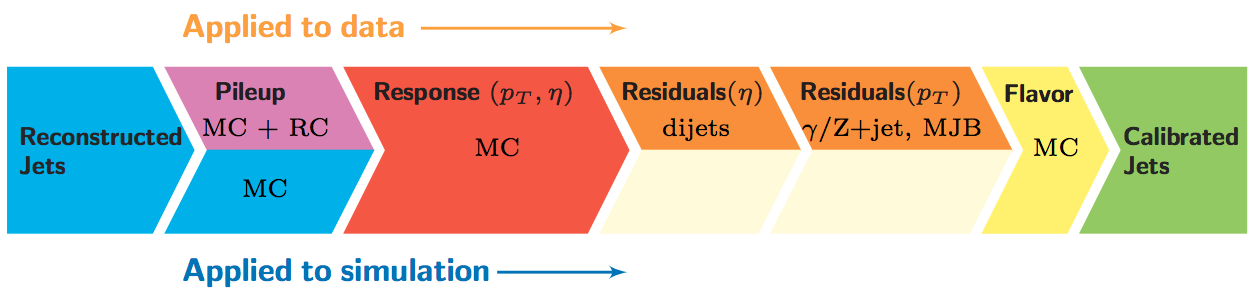
\includegraphics[width=0.8\textwidth]{/Users/db0268/Desktop/Thesis/Figures/Event_JESFlow.png}
	\caption[A schematic showing the factorised steps to correct the energy scale of a jet. These consist of a pileup correction, detector response correction with additional residuals applied in data and optional flavour corrections.]{A schematic showing the factorised steps to correct the energy scale of a jet. These consist of a pileup correction, detector response correction with additional residuals applied in data and optional flavour corrections. Schematic taken from~\cite{Event:JEC}.}
	\label{fig:JESFlow}
\end{figure}

The first correction is applied to counter additional energy in the jet, known as \textit{offset energy}, coming from pileup and the underlying event. 
%+noise
In-time pileup is already partially removed by the charged hadron subtraction algorithm, which accounts for $\sim50\%$ of the offset energy.
The rest of the diffuse neutral energy and out-of-time pileup is removed on an event-by-event basis using the \textit{hybrid jet area method} dependent on the offset energy density $\rho$ and the effective jet area $A^{\mathrm{jet}}$.
The variable $\rho$ is taken as the median of the energies present in a grid of $\eta - \phi$ cells.
The use of the median creates an insensitivity to hard jets in the event.   
The correction is applied as
\begin{equation}
	\pt^{\mathrm{corr}} = \pt^{\mathrm{uncorr}} - \
	A^{\mathrm{jet}}\Big(\rho_{0}(\eta) + \
	\rho\beta(\eta)[1+\gamma(\eta)\log{(\pt^{\mathrm{uncorr}})]\Big)},
\end{equation}
where $\rho_{0}, \beta$ and $\gamma$ are $\eta$ dependent variables which are estimated from simulated \acrshort{qcd} dijets processed with and without pileup overlay and parametrise the shape of the offset energy distribution.
Residual corrections applied to data which stem from differences between the data and the detector simulation are determined using the random cone method on zero-bias events.
% data and simulation of rho???
Zero-bias events are events in which there is no hard-scattering process and so any jet energies should come from pileup provided the electronic noise is small.
The random cone method estimates $\rho$ by clustering many jets around random cones mapping all $\eta-\phi$ space and taking the average jet \pt{}.
This correction removes any dependence of the jet energy on the luminosity for the subsequent corrections.
% ue contained in rho0, 
% correction for nonuniformity in IT and OOT offsets wrt eta, beta
% residual correction factor depending on log jet pt dependence, gamma

Next, a second set of corrections are applied to both data and simulation to create a uniform jet energy response with respect to \pt{} and $\eta$.
This is done using a simulated \acrshort{qcd} dijet sample to compare the \pt{} of the reconstructed jets to the particle-level jets.
The response is defined as the ratio of the average reconstructed jet \pt{} to the average particle-level jet \pt{}.
The simulated jet response at the end of Run I, which is used in the \acrshort{jec} applied in this thesis, can be seen in Fig.~\ref{fig:JES}.
Preliminary measurements of the simulated jet energy response for detector conditions during 2016 are given in~\cite{Event:JEC2016RunII}.
\begin{figure}[htpb!]
	\centering
	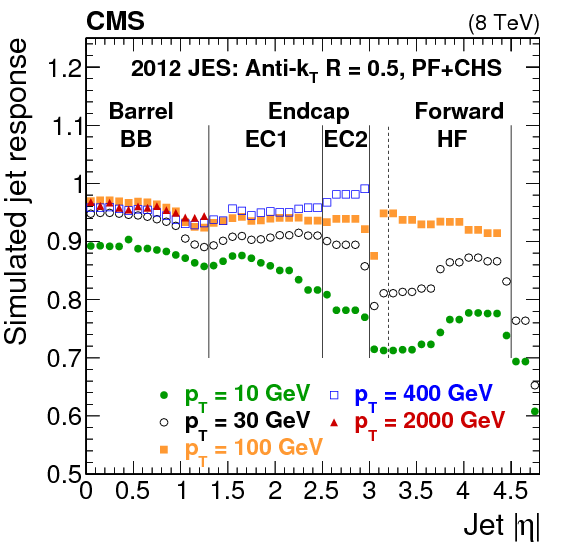
\includegraphics[width=0.55\textwidth]{/Users/db0268/Desktop/Thesis/Figures/Event_JESused.png}
	\caption[The simulated jet energy response as a function of \pt{} and $\eta$. These corrections are based on the status of the detector after the end of Run I.]{The simulated jet energy response as a function of \pt{} and $\eta$. These corrections are based on the status of the detector after the end of Run I~\cite{Event:JEC}.}
	\label{fig:JES}
\end{figure}

Residual corrections are calculated from data and applied to correct small differences seen in the jet energy response between simulation and data.
These consist of a $\eta$ dependent correction determined from \acrshort{qcd} dijet events relative to a barrel reference jet of similar \pt{} and a correction on jet energy scale with respect to \pt{}.
The \pt{} correction is based on \Zboson/\photon{}+jets and \acrshort{qcd} multijet events. 
Finally, optional corrections based on the response of different particle flavours can be applied.
These corrections are derived from simulation and are not applied in this thesis.

As well as variations present in the jet energy scale, variations are also present in the jet energy resolution (\acrshort{jer}).
The \acrshort{jer} scale factors $\mathrm{SF}_{\mathrm{JER}}$ are determined from the ratio of data to simulated \acrshort{qcd} dijet events with respect to \pt{}, $\eta$ and additional interaction vertices.
The \acrshort{jer} of jets in simulation $\sigma_\mathrm{JER}^{\mathrm{sim}}$ is also better than that seen in data and so must be smeared to match.
A hybrid of two approaches is used to correct and smear the resolution in simulation.
If a reconstructed jet is well matched to a particle-level jet such that 
\begin{equation*}
	\Delta R < \frac{R_\mathrm{cone}}{2}
\end{equation*}
and 
\begin{equation}
	\abs{\pt - \pt^\mathrm{ptcl}} < 3\,\sigma_\mathrm{JER}^{\mathrm{sim}}\,\pt,
\end{equation}
 then the jet \pt{} is rescaled by
\begin{equation*}
	1+(\mathrm{SF}_{\mathrm{JER}}-1)\frac{\pt-\pt^{\mathrm{ptcl}}}{\pt}.
\end{equation*}
However, if the jet is not matched then a stochastic smearing is applied
\begin{equation*}
	1 + \mathcal{N}(0,\sigma_\mathrm{JER}^{\mathrm{sim}}) \sqrt{\max(\mathrm{SF}_{\mathrm{JER}}^2 - 1, 0)}.
\end{equation*}
$\mathcal N(0,\sigma_\mathrm{JER}^{\mathrm{sim}})$ represents a random number sampled from a Gaussian distribution centred on 0 with a standard deviation given by the \acrshort{jer} in simulation.

% be careful  - this is the relative JER so Delta pt over pt
% section jet_energy_corrections (end)
% \begin{figure}[htpb]
% 	\centering
% 	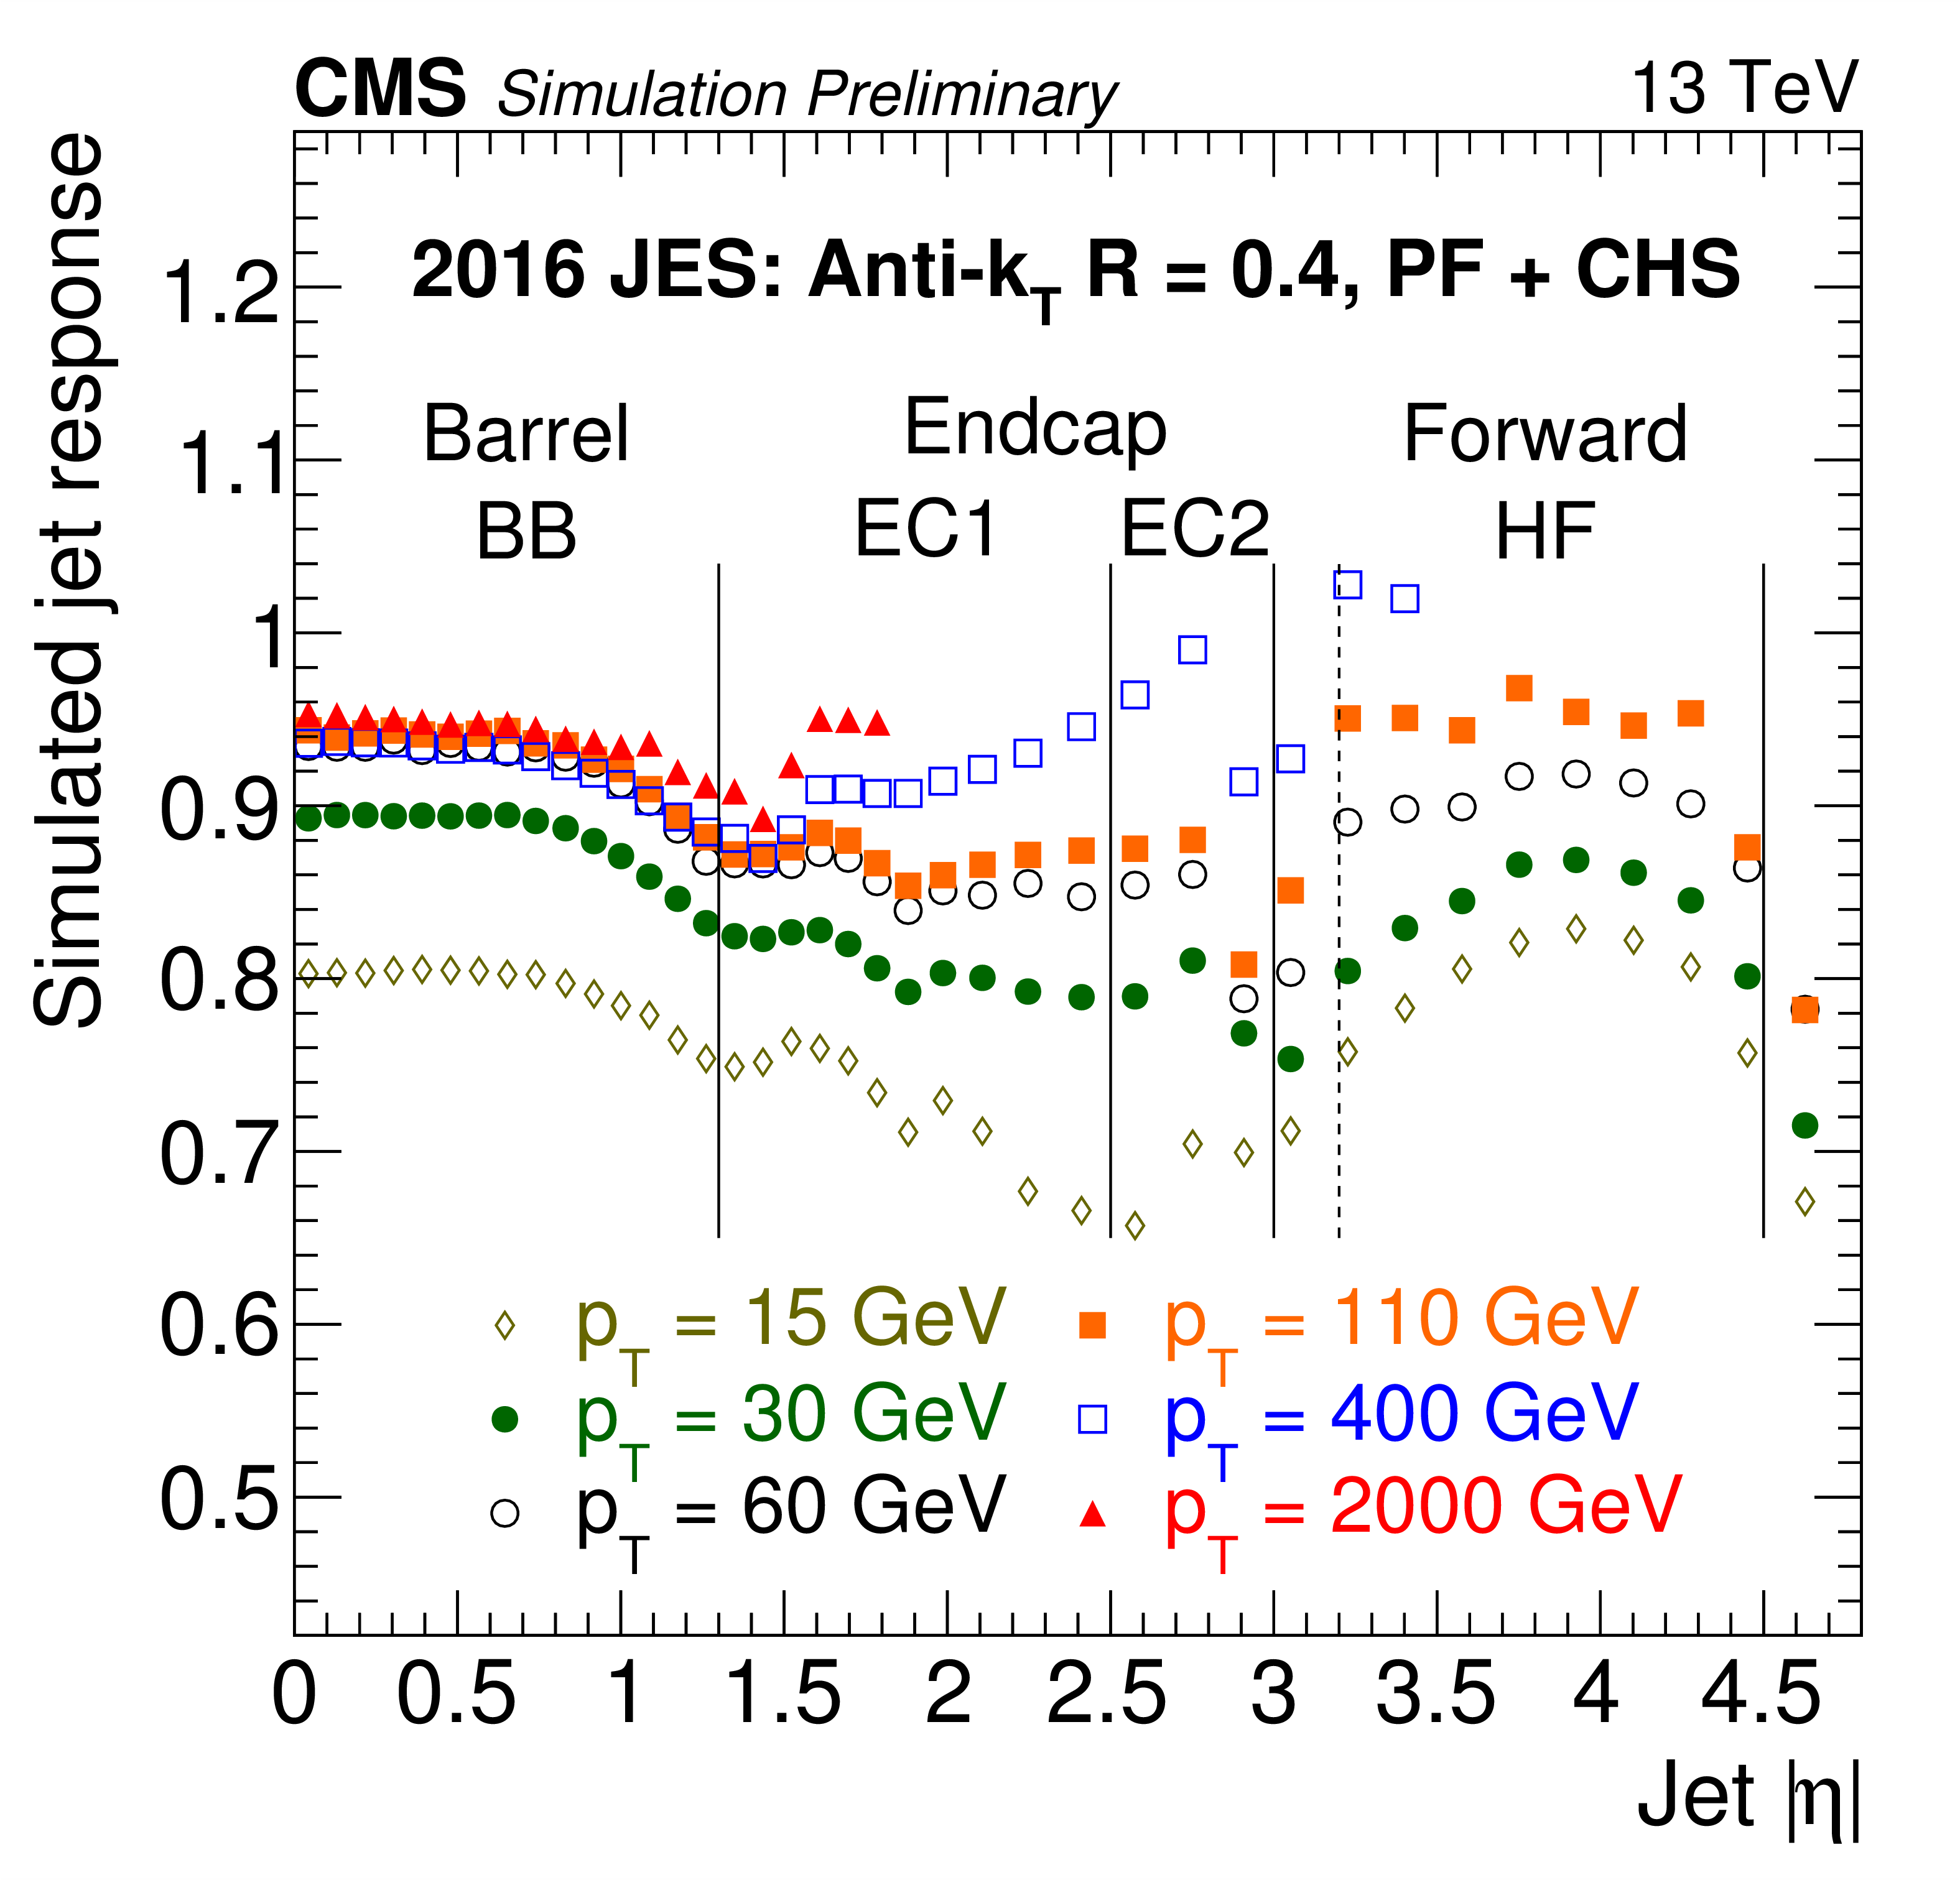
\includegraphics[width=0.49\textwidth]{/Users/db0268/Desktop/Thesis/Figures/Event_JES.png}
% 	\caption[.]{.~\cite{JEC2016RunII}}
% 	\label{fig:JES2016RunII}
% \end{figure}

\section{Reweighting from additional interactions} % (fold)
\label{sub:reweighting_from_additional_interactions}

The number of additional interactions in simulation differs to that seen in data.
The left panel of Fig.~\ref{fig:PU} shows the difference seen in the number of reconstructed vertices after full event selection.
The true vertex multiplicity distribution in simulation is reweighted to match that seen in data.
This is done by creating a scale factor from the number of additional interactions seen in data and simulation.
The true distribution of the number of additional interactions in data $N_{\mathrm{PU}}^{\mathrm{Data}}$ is estimated every bunch crossing using
\begin{equation*}
	N_{i}^{\mathrm{True}} = \sigma_{\mathrm{minbias}} \times \Lum_{i}.
\end{equation*}
The parameter $\sigma_{\mathrm{minbias}}$ is the total inelastic cross section taken as 69.2\mb{} and $\Lum_{i}$ the instantaneous luminosity in the luminosity section $i$.
The true distribution of additional interactions in simulation $N_{\mathrm{PU}}^{\mathrm{Sim}}$ also includes interactions from out-of-time pileup.
The number of reconstructed vertices in simulation is then reweighted by 
\begin{equation}
	\frac{N_{\mathrm{PU}}^{\mathrm{Data}}}{N_{\mathrm{PU}}^{\mathrm{Sim}}},
\end{equation}
and the application is shown in the right panel of Fig.~\ref{fig:PU}.
While a discrepancy is seen in the reweighting, the distributions of the vertex multiplicities matches when considering the uncertainties on $\sigma_{\mathrm{minbias}}$ ($\pm4.6\%$).

\begin{figure}[htpb]
	\centering
	\includegraphics[width=0.49\textwidth]{/Users/db0268/Mount/SoolinScratch/DPS/DPSTestingGround/DailyPythonScripts/data_thesis/plots/control_plots/Nominal/Control/Ref_selection/COMBINED_NPUNoWeight_2orMoreBtags_with_ratio}
	\includegraphics[width=0.49\textwidth]{/Users/db0268/Mount/SoolinScratch/DPS/DPSTestingGround/DailyPythonScripts/data_thesis/plots/control_plots/Nominal/Control/Ref_selection/COMBINED_NPU_2orMoreBtags_with_ratio}
	\caption[A plot showing the distribution of the number of reconstructed primary vertices in simulation and data. The left panel shows the distribution before pileup reweighting and the right panel after.]{A plot showing the distribution of the number of reconstructed primary vertices in simulation and data. The left panel shows the distribution before pileup reweighting and the right panel after.}
	\label{fig:PU}
\end{figure}
% again minbias = total inelastic cross section, L = instantaneous Lumi.
% Alternate method is to count number of reconstructed primary vertices in a series of events. The average number of additional vertices corresponds linearly to the number of additional interactions, modulo the ~70% vertex reconstruction efficiency. So, the average number of reconstructed vertices divided by 0.7 is a good estimate of the number of additional interactions present in one LumiSection.
% section reweighting_from_additional_interactions (end)

\section{Reweighting from b jet identification} % (fold)
\label{sub:reweighting_from_b_jet_identification}

% The CSVv2 algorithm response of jets in data and simulation is not equivalent and so scale factors, derived in TODO, are applied 
% WP-> 70pc eff. Calc our own->70pc
The \bquark{} jet identification efficiencies for a given configuration of jets in data and simulation are different.
The simulation is corrected to match data by applying a weight
\begin{equation*}
	w = \frac{P(\mathrm{Data})}{P(\mathrm{Sim})},
\end{equation*}
where
\begin{equation*}
	P(\mathrm{Sim}) = \prod_{i\text{ = tagged}}\epsilon_{i}\prod_{j\text{ = not tagged}}(1 - \epsilon_{j})
\end{equation*}
and
\begin{equation*}
	P(\mathrm{Data}) = \prod_{i\text{ = tagged}}\mathrm{SF}_{i}\epsilon_{i}\prod_{j\text{ = not tagged}}(1 - \mathrm{SF}_{j}\epsilon_{j}).
\end{equation*}
The parameters $\epsilon_{i}$ and $\mathrm{SF}_{i}$ are the \bquark{} quark tagging efficiency and scale factor ($\epsilon_{\mathrm{DATA}}/\epsilon_{\mathrm{MC}}$) for the jet $i$, respectively.
The scale factors applied to the \bquark{} and light flavour jets in this thesis are derived in~\cite{Event:BTV}.

Both the \bquark{} tagging scale factors and efficiencies are calculated and applied as functions of \pt{}, $\eta$ and flavour (\bquark{}, \cquark{}, \udsg{}).
The \bquark{} jet tagging efficiency and light jet mis-tagging efficiencies are calculated from the \powhegpythia{} \ttbar{} simulation.
They are taken as the fraction of tagged jets over the total number of \bquark{} jets.
Figure~\ref{fig:BTag} shows the \bquark{} quark jet tagging efficiencies, which for genuine \bquark{} jets is $\approx70\%$ and for misidentified jets from light quarks is $\approx1\%$.
\begin{figure}[htpb]
	\centering
	\includegraphics[width=0.49\textwidth]{/Users/db0268/Mount/SoolinScratch/DPS/DPSTestingGround/DailyPythonScripts/plots/BTagEfficiency/pt_efficiency}
	\includegraphics[width=0.49\textwidth]{/Users/db0268/Mount/SoolinScratch/DPS/DPSTestingGround/DailyPythonScripts/plots/BTagEfficiency/eta_efficiency}
	\caption[The left panel shows the \bquark{} tagging efficiency with respect to jet \pt{} and the right panel with respect to jet $\eta$. Both panels show the efficiencies separated into \bquark{}, \cquark{} and light flavours.]{The left panel shows the \bquark{} tagging efficiency with respect to jet \pt{} and the right panel with respect to jet $\eta$. Both panels show the efficiencies separated into \bquark{}, \cquark{} and light flavours.}
	\label{fig:BTag}
\end{figure}

Figure~\ref{fig:BWeight} shows the \bquark{} jet multiplicity after full event selection before applying the \bquark{} jet reweighting in the left panel and after in the right panel.
The discrepancy in the first bin is covered by the uncertainty in multijet \acrshort{qcd}, taken from simulation.
The size of the multijet \acrshort{qcd} normalisation uncertainty is $\approx60\%$ motivated in Sec.~\ref{sec:multijet_qcd}.
\begin{figure}[htpb]
	\centering
	\includegraphics[width=0.49\textwidth]{/Users/db0268/Mount/SoolinScratch/DPS/DPSTestingGround/DailyPythonScripts/data_thesis/plots/control_plots/Nominal/Control/Ref_selection/COMBINED_NBJetsNoWeight_2orMoreBtags_with_ratio}
	\includegraphics[width=0.49\textwidth]{/Users/db0268/Mount/SoolinScratch/DPS/DPSTestingGround/DailyPythonScripts/data_thesis/plots/control_plots/Nominal/Control/Ref_selection/COMBINED_NBJets_2orMoreBtags_with_ratio}	
	\caption[The left panel shows the \bquark{} jet multiplicity distribution before reweighting and the right panel after reweighting.]{The left panel shows the \bquark{} jet multiplicity distribution before reweighting and the right panel after reweighting.}
	\label{fig:BWeight}
\end{figure}
% section reweighting_from_b_jet_identification (end)

\section{Reweighting from leptons} % (fold)
\label{sub:reweighting_from_leptons}

The reconstruction, identification and triggering efficiencies of leptons are measured in data and corrected in simulation to match data.
The electron efficiencies and scale factors are derived using the tag-and-probe method following prescriptions defined in~\cite{Event:eSFMethod} using the clustering algorithm described in~\cite{Event:PFlow} and are presented in~\cite{Event:ElectronSF}.
Muon scale factors are measured in a similar manner and are presented in~\cite{Event:MuonSF,Event:MuonTrigSF}.
In both channels the efficiencies are measured from events containing a \Zboson{} boson and the corrective scale factors are applied as a function of \pt{} and supercluster pseudorapidity \sceta{}.
The total lepton scale factors vary between 0.95 and 1.

The electron \acrshort{id} scale factors are produced in bins of \sceta{} coarse enough to have significant effects on the distribution of \LETA{}.
This is because the high resolution of \LETA{} allows for fine-bin measurements and the application of the scale factors would cover several bins.
It is therefore not appropriate to use these electron \acrshort{id} scale factors for the \LETA{} event variable.
They are rederived with respect to the finer binning used in the production of the electron reconstruction scale factors for an identical \pt{} range.
An identical method used for the original scale factors is used in the rederivation.
Figure~\ref{fig:eIDSF} shows the efficiency of the electron \acrshort{id} in data (points) and simulation (dashes) and the scale factor to be applied is the ratio.
This new scale factor is only applied for the \LETA{} differential measurements.
\begin{figure}[htpb]
	\centering
	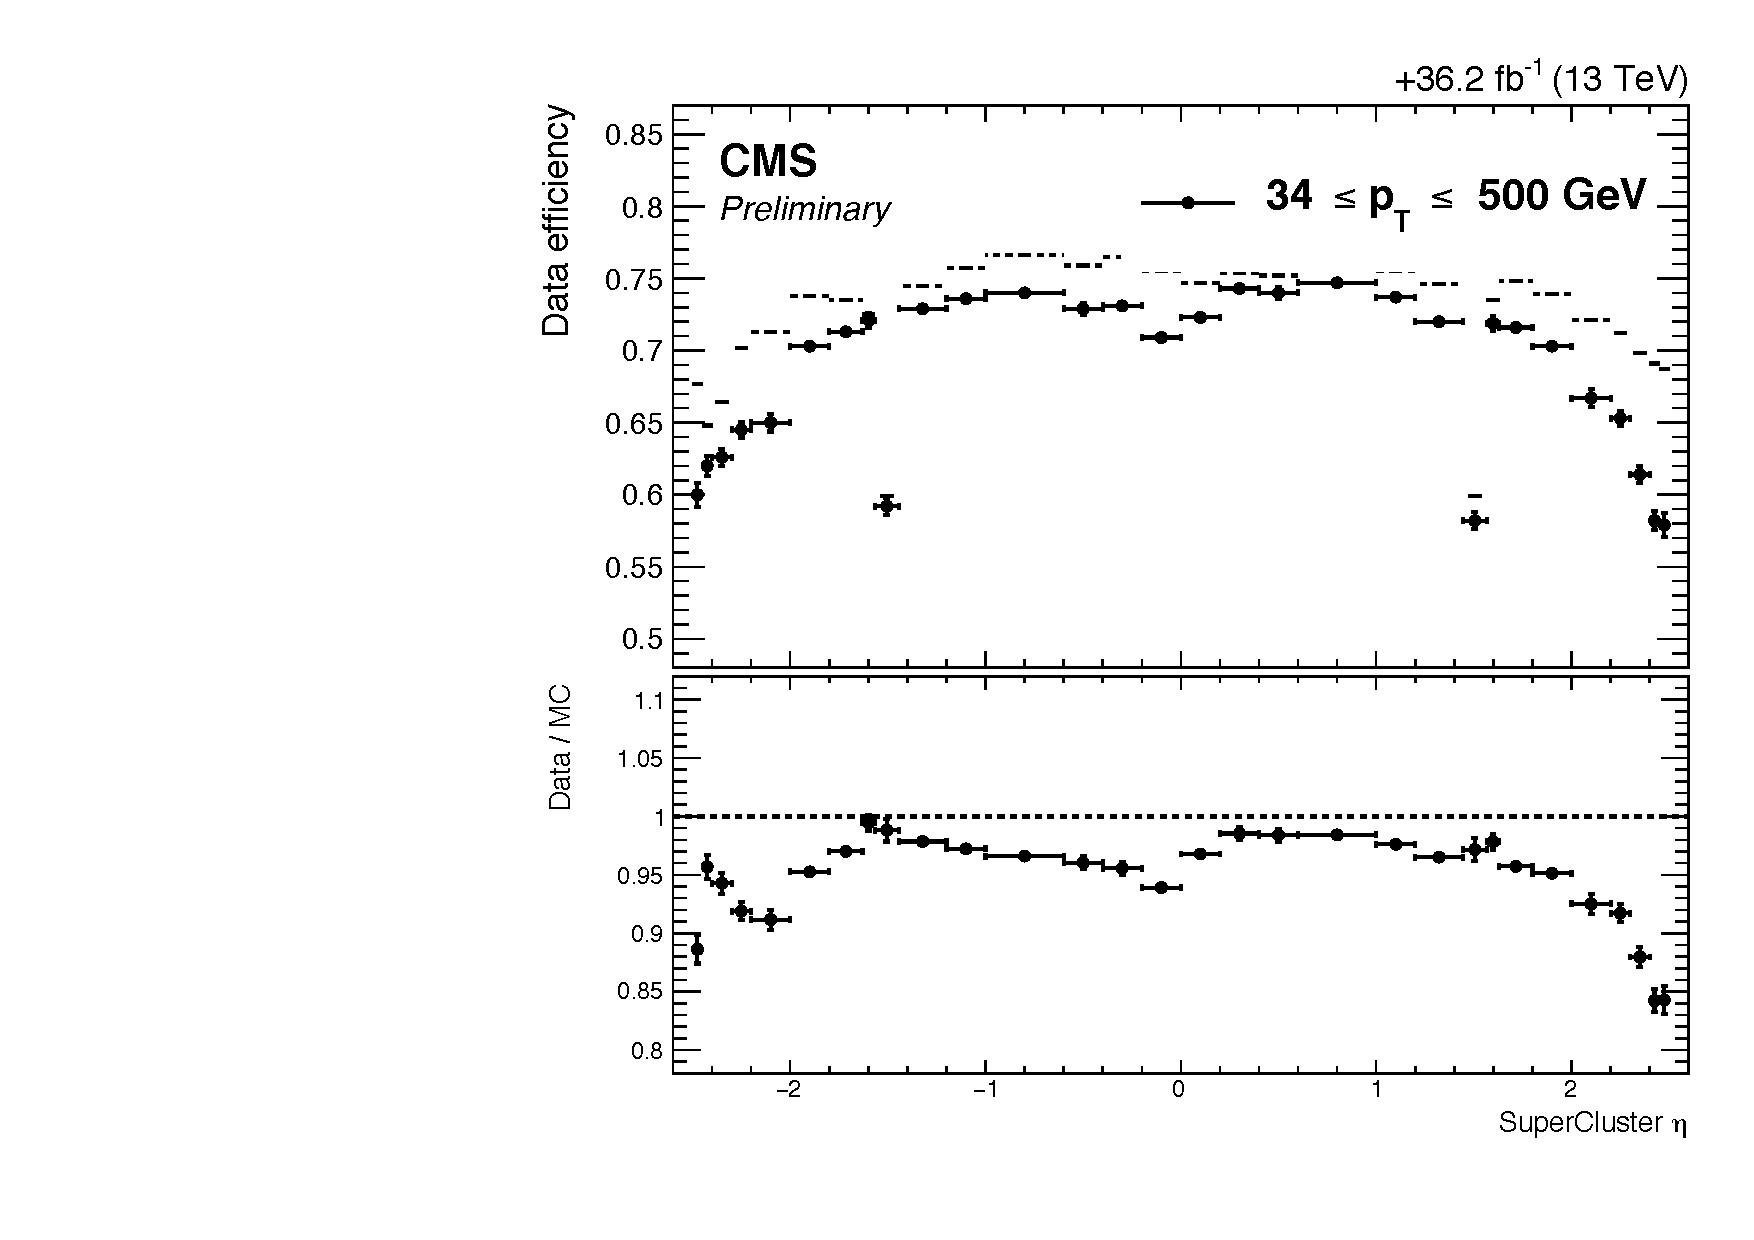
\includegraphics[width=0.7\textwidth]{Figures/Event_eIDSF.pdf}
	\caption[The electron identification efficiency for data and simulation calculated with events with a \Zboson{} boson present using the tag-and-probe method. The ratio of the two efficiencies is the finer binned scale factors applied in the \LETA{} measurements.]{The electron identification efficiency for data and simulation calculated with events with a \Zboson{} boson present using the tag-and-probe method. The ratio of the two efficiencies is the finer binned scale factors applied in the \LETA{} measurements.}
	\label{fig:eIDSF}
\end{figure}
% section reweighting_from_leptons (end)

\section{Multijet QCD} % (fold)
\label{sec:multijet_qcd}

The multijet \acrshort{qcd} background is notoriously hard to model and as such a data driven approach is used to estimate its contribution in the signal region from an orthogonal control region.
The control region is designed to be enhanced in multijet \acrshort{qcd} and to achieve that in the \eJets{} channel the \acrshort{qcd} event selection inverts the isolation requirement in the electron \acrshort{id} and requires exactly zero \bquark{} jets.
For the \muJets{} channel the control region event selection requires $0.15<\Irel<0.30$ and zero \bquark{} tagged jets.
In these control regions, the contribution of \ttbar{}, single top quark, and \Vjets{} background is estimated from simulation to be $\approx15-20\%$.
These estimations are subtracted from the data to extract the shape of the multijet \acrshort{qcd} in data.
The \acrshort{qcd} distributions are then scaled to the signal region by a transfer factor derived from simulation
\begin{equation*}
	t_{f}=\frac{N^{\mathrm{Signal}}_{\QCD,\,\mathrm{MC}}}{N^{\mathrm{Control}}_{\QCD,\,\mathrm{MC}}},
\end{equation*}
where $N^{\mathrm{Signal}}_{\QCD,\,\mathrm{MC}}$ and $N^{\mathrm{Control}}_{\QCD,\,\mathrm{MC}}$ are the total normalisation of the \acrshort{qcd} simulation in the signal and control regions respectively.
Transfer factors for all nominal control regions are shown in Tab.~\ref{tb:qcdTF}.
\begin{table}[h!]
    \centering
    \caption{The transfer factors to the signal region from the four multijet \QCD{} control regions.}
    \label{tb:qcdTF}
    \begin{tabular}{lc}
            \textbf{Control region}     			&	\textbf{Transfer factor} \\
            \hline
            Non-isolated electron					&	0.27 \\
            Conversion electron						&   0.03 \\
            Non-isolated muon $0.15<\Irel<0.30 $ 	& 	0.11 \\
            Non-isolated muon $0.30<\Irel<\infty$ 	& 	0.08 \\
    \end{tabular} \\
\end{table}


To validate the use of the nominal control region, the \acrshort{qcd} contribution is estimated in an alternate control region and compared to background subtracted data in that control region.
The comparison can also yield the shape and normalisation uncertainties on the data driven \acrshort{qcd} estimate.
In the \eJets{} channel the alternate control region uses an electron ID where the conversion veto or missing hits criteria has been inverted and in the \muJets{} channel the $0.30<\Irel<\infty$ region is used.
Both still require exactly zero \bquark{} tagged jets.
The data-simulation comparison plots of the event variables in the multijet \acrshort{qcd} control regions for the \eJets{} channel are shown in Figs.~\ref{fig:QCDeNonIso} and~\ref{fig:QCDeConv} and for the \muJets{} channel in Figs.~\ref{fig:QCDmuNonIso2} and~\ref{fig:QCDmuNonIso}.

Figures~\ref{fig:QCDeValid} and~\ref{fig:QCDmuValid} show the data-driven \acrshort{qcd} estimates in the alternate control region compared to the \acrshort{qcd} calculated by subtracting backgrounds from the data in the alternate control region.
The differences between the two predictions show the accuracy of the prediction, which is expected to be similar for the prediction in the signal region.
The uncertainty of the \acrshort{qcd} prediction in the signal region can therefore be taken from the discrepancies seen in this control region.
Any offset from unity in the ratio of the two \acrshort{qcd} yields gives the normalisation uncertainty, taken as $\pm60\%$ (gold band) and the spread of the ratio gives the shape uncertainty, taken as $\pm30\%$ (grey band).
The regions where the ratio is outside these uncertainty bands the expected contribution of \acrshort{qcd} is negligible, \eg{} at high \ptmiss{}.
\begin{figure}[hp!]
	\centering
	\includegraphics[width=0.32\textwidth]{/Users/db0268/Mount/SoolinScratch/DPS/DPSTestingGround/DailyPythonScripts/data_thesis/plots/control_plots/Nominal/QCDControl/electronQCDNonIso/electronQCDNonIso_logYNJets_0btag_with_ratio.png}
	\includegraphics[width=0.32\textwidth]{/Users/db0268/Mount/SoolinScratch/DPS/DPSTestingGround/DailyPythonScripts/data_thesis/plots/control_plots/Nominal/QCDControl/electronQCDNonIso/electronQCDNonIso_HT_0btag_with_ratio.png}
	\includegraphics[width=0.32\textwidth]{/Users/db0268/Mount/SoolinScratch/DPS/DPSTestingGround/DailyPythonScripts/data_thesis/plots/control_plots/Nominal/QCDControl/electronQCDNonIso/electronQCDNonIso_ST_0btag_with_ratio.png} \\
	\includegraphics[width=0.32\textwidth]{/Users/db0268/Mount/SoolinScratch/DPS/DPSTestingGround/DailyPythonScripts/data_thesis/plots/control_plots/Nominal/QCDControl/electronQCDNonIso/electronQCDNonIso_MET_0btag_with_ratio.png}
	\includegraphics[width=0.32\textwidth]{/Users/db0268/Mount/SoolinScratch/DPS/DPSTestingGround/DailyPythonScripts/data_thesis/plots/control_plots/Nominal/QCDControl/electronQCDNonIso/electronQCDNonIso_WPT_0btag_with_ratio.png} \\
	\includegraphics[width=0.32\textwidth]{/Users/db0268/Mount/SoolinScratch/DPS/DPSTestingGround/DailyPythonScripts/data_thesis/plots/control_plots/Nominal/QCDControl/electronQCDNonIso/electronQCDNonIso_LeptonPt_0btag_with_ratio.png} 
	\includegraphics[width=0.32\textwidth]{/Users/db0268/Mount/SoolinScratch/DPS/DPSTestingGround/DailyPythonScripts/data_thesis/plots/control_plots/Nominal/QCDControl/electronQCDNonIso/electronQCDNonIso_AbsLeptonEta_0btag_with_ratio.png}
	\includegraphics[width=0.32\textwidth]{/Users/db0268/Mount/SoolinScratch/DPS/DPSTestingGround/DailyPythonScripts/data_thesis/plots/control_plots/Nominal/QCDControl/electronQCDNonIso/electronQCDNonIso_relIso_0btag_with_ratio.png}
	\caption[The distributions of the event variables and $I_{\mathrm{rel}}$ in the non-isolated electron control region. The ratio of the number of events in data to that in simulation is shown below each of the distributions, with the statistical uncertainty in data given by the vertical error bars.]{The distributions of the event variables and $I_{\mathrm{rel}}$ in the non-isolated electron control region. The ratio of the number of events in data to that in simulation is shown below each of the distributions, with the statistical uncertainty in data given by the vertical error bars.}
	\label{fig:QCDeNonIso}
\end{figure}
\begin{figure}[hp!]
	\centering
	\includegraphics[width=0.32\textwidth]{/Users/db0268/Mount/SoolinScratch/DPS/DPSTestingGround/DailyPythonScripts/data_thesis/plots/control_plots/Nominal/QCDControl/electronQCDConversions/electronQCDConversions_logYNJets_0btag_with_ratio.png}
	\includegraphics[width=0.32\textwidth]{/Users/db0268/Mount/SoolinScratch/DPS/DPSTestingGround/DailyPythonScripts/data_thesis/plots/control_plots/Nominal/QCDControl/electronQCDConversions/electronQCDConversions_HT_0btag_with_ratio.png}
	\includegraphics[width=0.32\textwidth]{/Users/db0268/Mount/SoolinScratch/DPS/DPSTestingGround/DailyPythonScripts/data_thesis/plots/control_plots/Nominal/QCDControl/electronQCDConversions/electronQCDConversions_ST_0btag_with_ratio.png} \\
	\includegraphics[width=0.32\textwidth]{/Users/db0268/Mount/SoolinScratch/DPS/DPSTestingGround/DailyPythonScripts/data_thesis/plots/control_plots/Nominal/QCDControl/electronQCDConversions/electronQCDConversions_MET_0btag_with_ratio.png}
	\includegraphics[width=0.32\textwidth]{/Users/db0268/Mount/SoolinScratch/DPS/DPSTestingGround/DailyPythonScripts/data_thesis/plots/control_plots/Nominal/QCDControl/electronQCDConversions/electronQCDConversions_WPT_0btag_with_ratio.png} \\
	\includegraphics[width=0.32\textwidth]{/Users/db0268/Mount/SoolinScratch/DPS/DPSTestingGround/DailyPythonScripts/data_thesis/plots/control_plots/Nominal/QCDControl/electronQCDConversions/electronQCDConversions_LeptonPt_0btag_with_ratio.png} 
	\includegraphics[width=0.32\textwidth]{/Users/db0268/Mount/SoolinScratch/DPS/DPSTestingGround/DailyPythonScripts/data_thesis/plots/control_plots/Nominal/QCDControl/electronQCDConversions/electronQCDConversions_AbsLeptonEta_0btag_with_ratio.png}
	\includegraphics[width=0.32\textwidth]{/Users/db0268/Mount/SoolinScratch/DPS/DPSTestingGround/DailyPythonScripts/data_thesis/plots/control_plots/Nominal/QCDControl/electronQCDConversions/electronQCDConversions_relIso_0btag_with_ratio.png}
	\caption[The distributions of the event variables and $I_{\mathrm{rel}}$ in the conversion electron control region. The ratio of the number of events in data to that in simulation is shown below each of the distributions, with the statistical uncertainty in data given by the vertical error bars.]{The distributions of the event variables and $I_{\mathrm{rel}}$ in the conversion electron control region. The ratio of the number of events in data to that in simulation is shown below each of the distributions, with the statistical uncertainty in data given by the vertical error bars.}
	\label{fig:QCDeConv}
\end{figure}
\begin{figure}[hp!]
	\centering
	\includegraphics[width=0.32\textwidth]{/Users/db0268/Mount/SoolinScratch/DPS/DPSTestingGround/DailyPythonScripts/data_thesis/plots/control_plots/Nominal/QCDControl/muonQCDNonIso2/muonQCDNonIso2_logYNJets_0btag_with_ratio.png}
	\includegraphics[width=0.32\textwidth]{/Users/db0268/Mount/SoolinScratch/DPS/DPSTestingGround/DailyPythonScripts/data_thesis/plots/control_plots/Nominal/QCDControl/muonQCDNonIso2/muonQCDNonIso2_HT_0btag_with_ratio.png}
	\includegraphics[width=0.32\textwidth]{/Users/db0268/Mount/SoolinScratch/DPS/DPSTestingGround/DailyPythonScripts/data_thesis/plots/control_plots/Nominal/QCDControl/muonQCDNonIso2/muonQCDNonIso2_ST_0btag_with_ratio.png} \\
	\includegraphics[width=0.32\textwidth]{/Users/db0268/Mount/SoolinScratch/DPS/DPSTestingGround/DailyPythonScripts/data_thesis/plots/control_plots/Nominal/QCDControl/muonQCDNonIso2/muonQCDNonIso2_MET_0btag_with_ratio.png}
	\includegraphics[width=0.32\textwidth]{/Users/db0268/Mount/SoolinScratch/DPS/DPSTestingGround/DailyPythonScripts/data_thesis/plots/control_plots/Nominal/QCDControl/muonQCDNonIso2/muonQCDNonIso2_WPT_0btag_with_ratio.png} \\
	\includegraphics[width=0.32\textwidth]{/Users/db0268/Mount/SoolinScratch/DPS/DPSTestingGround/DailyPythonScripts/data_thesis/plots/control_plots/Nominal/QCDControl/muonQCDNonIso2/muonQCDNonIso2_LeptonPt_0btag_with_ratio.png} 
	\includegraphics[width=0.32\textwidth]{/Users/db0268/Mount/SoolinScratch/DPS/DPSTestingGround/DailyPythonScripts/data_thesis/plots/control_plots/Nominal/QCDControl/muonQCDNonIso2/muonQCDNonIso2_AbsLeptonEta_0btag_with_ratio.png}
	\includegraphics[width=0.32\textwidth]{/Users/db0268/Mount/SoolinScratch/DPS/DPSTestingGround/DailyPythonScripts/data_thesis/plots/control_plots/Nominal/QCDControl/muonQCDNonIso2/muonQCDNonIso2_relIso_0btag_with_ratio.png}
	\caption[The distributions of the event variables and $I_{\mathrm{rel}}$ in the non-isolated $(0.15 < I_{\mathrm{rel}} < 0.30)$ muon control region. The ratio of the number of events in data to that in simulation is shown below each of the distributions, with the statistical uncertainty in data given by the vertical error bars.]{The distributions of the event variables and $I_{\mathrm{rel}}$ in the non-isolated $(0.15 < I_{\mathrm{rel}} < 0.30)$ muon control region. The ratio of the number of events in data to that in simulation is shown below each of the distributions, with the statistical uncertainty in data given by the vertical error bars.}
	\label{fig:QCDmuNonIso2}
\end{figure}
\begin{figure}[hp!]
	\centering
	\includegraphics[width=0.32\textwidth]{/Users/db0268/Mount/SoolinScratch/DPS/DPSTestingGround/DailyPythonScripts/data_thesis/plots/control_plots/Nominal/QCDControl/muonQCDNonIso/muonQCDNonIso_logYNJets_0btag_with_ratio.png}
	\includegraphics[width=0.32\textwidth]{/Users/db0268/Mount/SoolinScratch/DPS/DPSTestingGround/DailyPythonScripts/data_thesis/plots/control_plots/Nominal/QCDControl/muonQCDNonIso/muonQCDNonIso_HT_0btag_with_ratio.png}
	\includegraphics[width=0.32\textwidth]{/Users/db0268/Mount/SoolinScratch/DPS/DPSTestingGround/DailyPythonScripts/data_thesis/plots/control_plots/Nominal/QCDControl/muonQCDNonIso/muonQCDNonIso_ST_0btag_with_ratio.png} \\
	\includegraphics[width=0.32\textwidth]{/Users/db0268/Mount/SoolinScratch/DPS/DPSTestingGround/DailyPythonScripts/data_thesis/plots/control_plots/Nominal/QCDControl/muonQCDNonIso/muonQCDNonIso_MET_0btag_with_ratio.png}
	\includegraphics[width=0.32\textwidth]{/Users/db0268/Mount/SoolinScratch/DPS/DPSTestingGround/DailyPythonScripts/data_thesis/plots/control_plots/Nominal/QCDControl/muonQCDNonIso/muonQCDNonIso_WPT_0btag_with_ratio.png} \\
	\includegraphics[width=0.32\textwidth]{/Users/db0268/Mount/SoolinScratch/DPS/DPSTestingGround/DailyPythonScripts/data_thesis/plots/control_plots/Nominal/QCDControl/muonQCDNonIso/muonQCDNonIso_LeptonPt_0btag_with_ratio.png} 
	\includegraphics[width=0.32\textwidth]{/Users/db0268/Mount/SoolinScratch/DPS/DPSTestingGround/DailyPythonScripts/data_thesis/plots/control_plots/Nominal/QCDControl/muonQCDNonIso/muonQCDNonIso_AbsLeptonEta_0btag_with_ratio.png}
	\includegraphics[width=0.32\textwidth]{/Users/db0268/Mount/SoolinScratch/DPS/DPSTestingGround/DailyPythonScripts/data_thesis/plots/control_plots/Nominal/QCDControl/muonQCDNonIso/muonQCDNonIso_relIso_0btag_with_ratio.png}
	\caption[The distributions of the event variables and $I_{\mathrm{rel}}$ in the non-isolated $(0.30 < I_{\mathrm{rel}} < \infty )$ muon control region. The ratio of the number of events in data to that in simulation is shown below each of the distributions, with the statistical uncertainty in data given by the vertical error bars.]{The distributions of the event variables and $I_{\mathrm{rel}}$ in the non-isolated $(0.30 < I_{\mathrm{rel}} < \infty )$ muon control region. The ratio of the number of events in data to that in simulation is shown below each of the distributions, with the statistical uncertainty in data given by the vertical error bars.}
	\label{fig:QCDmuNonIso}
\end{figure}

\begin{figure}[p]
	\centering
	\includegraphics[width=0.32\textwidth]{/Users/db0268/Mount/SoolinScratch/DPS/DPSTestingGround/DailyPythonScripts/plots/QCDvalidation/NJets_electron.pdf}
	\includegraphics[width=0.32\textwidth]{/Users/db0268/Mount/SoolinScratch/DPS/DPSTestingGround/DailyPythonScripts/plots/QCDvalidation/HT_electron.pdf} 
	\includegraphics[width=0.32\textwidth]{/Users/db0268/Mount/SoolinScratch/DPS/DPSTestingGround/DailyPythonScripts/plots/QCDvalidation/ST_electron.pdf} \\
	\includegraphics[width=0.32\textwidth]{/Users/db0268/Mount/SoolinScratch/DPS/DPSTestingGround/DailyPythonScripts/plots/QCDvalidation/MET_electron.pdf} 
	\includegraphics[width=0.32\textwidth]{/Users/db0268/Mount/SoolinScratch/DPS/DPSTestingGround/DailyPythonScripts/plots/QCDvalidation/WPT_electron.pdf} \\
	\includegraphics[width=0.32\textwidth]{/Users/db0268/Mount/SoolinScratch/DPS/DPSTestingGround/DailyPythonScripts/plots/QCDvalidation/lepton_pt_electron.pdf} 
	\includegraphics[width=0.32\textwidth]{/Users/db0268/Mount/SoolinScratch/DPS/DPSTestingGround/DailyPythonScripts/plots/QCDvalidation/abs_lepton_eta_coarse_electron.pdf}
	\caption[The prediction of multijet \QCD{} in the alternate control region from the nominal control region for each event variable in the electron channel. Also shown as a comparison is the data-subtracted \QCD{} estimate from the alternate control region. Below each of the distributions, the ratio of the two \QCD predictions is shown. This ratio gives an estimation of the \QCD{} normalisation uncertainty by the displacement from unity and was taken to be $\pm50\%$ shown by the gold band. The \QCD{} shape uncertainty is given by the spread of the ratio, taken to be $\pm30\%$ shown by the grey band.]{The prediction of multijet \QCD{} in the alternate control region from the nominal control region for each event variable in the electron channel. Also shown as a comparison is the data-subtracted \QCD{} estimate from the alternate control region. Below each of the distributions, the ratio of the two \QCD predictions is shown. This ratio gives an estimation of the \QCD{} normalisation uncertainty by the displacement from unity and was taken to be $\pm50\%$ shown by the gold band. The \QCD{} shape uncertainty is given by the spread of the ratio, taken to be $\pm30\%$ shown by the grey band.}
	\label{fig:QCDeValid}
\end{figure}

\begin{figure}[p]
	\centering
	\includegraphics[width=0.32\textwidth]{/Users/db0268/Mount/SoolinScratch/DPS/DPSTestingGround/DailyPythonScripts/plots/QCDvalidation/NJets_muon.pdf}
	\includegraphics[width=0.32\textwidth]{/Users/db0268/Mount/SoolinScratch/DPS/DPSTestingGround/DailyPythonScripts/plots/QCDvalidation/HT_muon.pdf} 
	\includegraphics[width=0.32\textwidth]{/Users/db0268/Mount/SoolinScratch/DPS/DPSTestingGround/DailyPythonScripts/plots/QCDvalidation/ST_muon.pdf} \\
	\includegraphics[width=0.32\textwidth]{/Users/db0268/Mount/SoolinScratch/DPS/DPSTestingGround/DailyPythonScripts/plots/QCDvalidation/MET_muon.pdf} 
	\includegraphics[width=0.32\textwidth]{/Users/db0268/Mount/SoolinScratch/DPS/DPSTestingGround/DailyPythonScripts/plots/QCDvalidation/WPT_muon.pdf} \\
	\includegraphics[width=0.32\textwidth]{/Users/db0268/Mount/SoolinScratch/DPS/DPSTestingGround/DailyPythonScripts/plots/QCDvalidation/lepton_pt_muon.pdf} 
	\includegraphics[width=0.32\textwidth]{/Users/db0268/Mount/SoolinScratch/DPS/DPSTestingGround/DailyPythonScripts/plots/QCDvalidation/abs_lepton_eta_coarse_muon.pdf}
	\caption[The prediction of multijet \QCD{} in the alternate control region from the nominal control region for each event variable in the muon channel. Also shown as a comparison is the data-subtracted \QCD{} estimate from the alternate control region. Below each of the distributions, the ratio of the two \QCD predictions is shown. This ratio gives an estimation of the \QCD{} normalisation uncertainty by the displacement from unity and was taken to be $\pm50\%$ shown by the gold band. The \QCD{} shape uncertainty is given by the spread of the ratio, taken to be $\pm30\%$ shown by the grey band.]{The prediction of multijet \QCD{} in the alternate control region from the nominal control region for each event variable in the muon channel. Also shown as a comparison is the data-subtracted \QCD{} estimate from the alternate control region. Below each of the distributions, the ratio of the two \QCD predictions is shown. This ratio gives an estimation of the \QCD{} normalisation uncertainty by the displacement from unity and was taken to be $\pm50\%$ shown by the gold band. The \QCD{} shape uncertainty is given by the spread of the ratio, taken to be $\pm30\%$ shown by the grey band.}
	\label{fig:QCDmuValid}
\end{figure}

% section multijet_qcd (end)
\newpage
\section{Data-simulation agreement in the signal region} % (fold)

% Figures~\ref{fig:eControlPlot1} and~\ref{fig:eControlPlot2} show the agreement between the data and the sum of the signal and background events from simulation in the \eJets{} channel and Figs.~\ref{fig:muControlPlot1} and~\ref{fig:muControlPlot2} for the \muJets{} channel.
Figures~\ref{fig:combControlPlot1} and~\ref{fig:combControlPlot2} show the agreement between the data and the sum of the signal and background events from simulation in the combined \eJets{} and \muJets{} channels.
All corrections previously described have been applied and the multijet \acrshort{qcd} contribution estimated from data.
A total of 662 381 events are measured in data, the composition of which is predicted to be $92.1\%$ \ttbar{} production, 4.4\% single top quark production, 2.1\% \Vjets{} production and 1.4\% from multijet \acrshort{qcd}.
The total level of agreement between simulation and data ($<0.2\%$) indicates the total cross section is compatible to that stated in Sec.~\ref{sub:top_quark_production}.
The statistical uncertainty in the data is given by vertical error bars.
The hatched bands shows the statistical uncertainty in the number of simulated events and experimental uncertainties combined in quadrature.
The set of experimental uncertainties include those from the \acrshort{jec} and \ptmiss{}, the luminosity, the pileup, lepton and \bquark{} tagging scale factors and the background predictions.
These uncertainties are explained in more detail in Sec.~\ref{sub:experimental_uncertainties}.
\label{sec:data_simulation_agreement_in_the_signal_region}
% \begin{figure}[hp]
% 	\centering
% 	\includegraphics[width=0.49\textwidth]{/Users/db0268/Mount/SoolinScratch/DPS/DPSTestingGround/DailyPythonScripts/data_thesis/plots/control_plots_with_systematic/logY/electron_NJets_with_ratio_logY.png} \\
% 	\includegraphics[width=0.49\textwidth]{/Users/db0268/Mount/SoolinScratch/DPS/DPSTestingGround/DailyPythonScripts/data_thesis/plots/control_plots_with_systematic/electron_HT_with_ratio.png}
% 	\includegraphics[width=0.49\textwidth]{/Users/db0268/Mount/SoolinScratch/DPS/DPSTestingGround/DailyPythonScripts/data_thesis/plots/control_plots_with_systematic/electron_ST_with_ratio.png} \\
% 	\caption[.]{.}
% 	\label{fig:eControlPlot1}
% \end{figure}
% \begin{figure}[hp]
% 	\centering
% 	\includegraphics[width=0.49\textwidth]{/Users/db0268/Mount/SoolinScratch/DPS/DPSTestingGround/DailyPythonScripts/data_thesis/plots/control_plots_with_systematic/electron_MET_with_ratio.png}
% 	\includegraphics[width=0.49\textwidth]{/Users/db0268/Mount/SoolinScratch/DPS/DPSTestingGround/DailyPythonScripts/data_thesis/plots/control_plots_with_systematic/electron_WPT_with_ratio.png} \\
% 	\includegraphics[width=0.49\textwidth]{/Users/db0268/Mount/SoolinScratch/DPS/DPSTestingGround/DailyPythonScripts/data_thesis/plots/control_plots_with_systematic/electron_lepton_pt_with_ratio.png} 
% 	\includegraphics[width=0.49\textwidth]{/Users/db0268/Mount/SoolinScratch/DPS/DPSTestingGround/DailyPythonScripts/data_thesis/plots/control_plots_with_systematic/electron_abs_lepton_eta_coarse_with_ratio.png}
% 	\caption[.]{.}
% 	\label{fig:eControlPlot2}
% \end{figure}
% \begin{figure}[hp]
% 	\centering
% 	\includegraphics[width=0.49\textwidth]{/Users/db0268/Mount/SoolinScratch/DPS/DPSTestingGround/DailyPythonScripts/data_thesis/plots/control_plots_with_systematic/logY/muon_NJets_with_ratio_logY.png} \\
% 	\includegraphics[width=0.49\textwidth]{/Users/db0268/Mount/SoolinScratch/DPS/DPSTestingGround/DailyPythonScripts/data_thesis/plots/control_plots_with_systematic/muon_HT_with_ratio.png}
% 	\includegraphics[width=0.49\textwidth]{/Users/db0268/Mount/SoolinScratch/DPS/DPSTestingGround/DailyPythonScripts/data_thesis/plots/control_plots_with_systematic/muon_ST_with_ratio.png} \\
% 	\caption[.]{.}
% 	\label{fig:muControlPlot1}
% \end{figure}
% \begin{figure}[hp]
% 	\centering
% 	\includegraphics[width=0.49\textwidth]{/Users/db0268/Mount/SoolinScratch/DPS/DPSTestingGround/DailyPythonScripts/data_thesis/plots/control_plots_with_systematic/muon_MET_with_ratio.png}
% 	\includegraphics[width=0.49\textwidth]{/Users/db0268/Mount/SoolinScratch/DPS/DPSTestingGround/DailyPythonScripts/data_thesis/plots/control_plots_with_systematic/muon_WPT_with_ratio.png} \\
% 	\includegraphics[width=0.49\textwidth]{/Users/db0268/Mount/SoolinScratch/DPS/DPSTestingGround/DailyPythonScripts/data_thesis/plots/control_plots_with_systematic/muon_lepton_pt_with_ratio.png} 
% 	\includegraphics[width=0.49\textwidth]{/Users/db0268/Mount/SoolinScratch/DPS/DPSTestingGround/DailyPythonScripts/data_thesis/plots/control_plots_with_systematic/muon_abs_lepton_eta_coarse_with_ratio.png}
% 	\caption[.]{.}
% 	\label{fig:muControlPlot2}
% \end{figure}
\begin{figure}[hp]
	\centering
	\includegraphics[width=0.49\textwidth]{/Users/db0268/Mount/SoolinScratch/DPS/DPSTestingGround/DailyPythonScripts/data_thesis/plots/control_plots_with_systematic/logY/COMBINED_NJets_with_ratio_logY.png} \\
	\includegraphics[width=0.49\textwidth]{/Users/db0268/Mount/SoolinScratch/DPS/DPSTestingGround/DailyPythonScripts/data_thesis/plots/control_plots_with_systematic/COMBINED_HT_with_ratio.png}
	\includegraphics[width=0.49\textwidth]{/Users/db0268/Mount/SoolinScratch/DPS/DPSTestingGround/DailyPythonScripts/data_thesis/plots/control_plots_with_systematic/COMBINED_ST_with_ratio.png} \\
	\caption[The distributions of \NJET{}, \HT{} and \ST{} after full event selection. The \ttbar{} simulation is normalised to the \NNLO{} prediction. The ratio of the number of events in data to that in simulation is shown below each of the distributions, with the statistical uncertainty in the data shown by the vertical error bars. The statistical uncertainty in the number of simulated events quadratically combined with the experimental uncertainties is shown by the hatched band.]{The distributions of \NJET{}, \HT{} and \ST{} after full event selection. The \ttbar{} simulation is normalised to the \NNLO{} prediction. The ratio of the number of events in data to that in simulation is shown below each of the distributions, with the statistical uncertainty in the data shown by the vertical error bars. The statistical uncertainty in the number of simulated events quadratically combined with the experimental uncertainties is shown by the hatched band.}
	\label{fig:combControlPlot1}
\end{figure}
\begin{figure}[hp]
	\centering
	\includegraphics[width=0.49\textwidth]{/Users/db0268/Mount/SoolinScratch/DPS/DPSTestingGround/DailyPythonScripts/data_thesis/plots/control_plots_with_systematic/COMBINED_MET_with_ratio.png}
	\includegraphics[width=0.49\textwidth]{/Users/db0268/Mount/SoolinScratch/DPS/DPSTestingGround/DailyPythonScripts/data_thesis/plots/control_plots_with_systematic/COMBINED_WPT_with_ratio.png} \\
	\includegraphics[width=0.49\textwidth]{/Users/db0268/Mount/SoolinScratch/DPS/DPSTestingGround/DailyPythonScripts/data_thesis/plots/control_plots_with_systematic/COMBINED_lepton_pt_with_ratio.png} 
	\includegraphics[width=0.49\textwidth]{/Users/db0268/Mount/SoolinScratch/DPS/DPSTestingGround/DailyPythonScripts/data_thesis/plots/control_plots_with_systematic/COMBINED_abs_lepton_eta_coarse_with_ratio.png}
	\caption[The distributions of \ptmiss, \WPT, \LPT and \LETA after full event selection. The \ttbar{} simulation is normalised to the \NNLO{} prediction. The ratio of the number of events in data to that in simulation is shown below each of the distributions, with the statistical uncertainty in the data shown by the vertical error bars. The statistical uncertainty in the number of simulated events quadratically combined with the experimental uncertainties is shown by the hatched band.]{The distributions of \ptmiss, \WPT, \LPT and \LETA after full event selection. The \ttbar{} simulation is normalised to the \NNLO{} prediction. The ratio of the number of events in data to that in simulation is shown below each of the distributions, with the statistical uncertainty in the data shown by the vertical error bars. The statistical uncertainty in the number of simulated events quadratically combined with the experimental uncertainties is shown by the hatched band.}
	\label{fig:combControlPlot2}
\end{figure}
The ratios of the event variables that are correlated to the \pt{} of the top quark show that the \ptTop{} is softer in data than in simulation.
This is a well known issue, with other analyses reporting the same effect. 
By reweighting the top quark \pt{} distribution to that measured by~\cite{TOP16007,TOP16008}, the slope observed in the ratio of these variables is corrected, as shown in Fig.~\ref{fig:combPtReweight}.

\begin{figure}[hp!]
	\centering	\includegraphics[width=0.65\textwidth]{/Users/db0268/Mount/SoolinScratch/DPS/DPSTestingGround/DailyPythonScripts/data_thesis/plots/control_plots_with_systematic/ptReweight/COMBINED_HT_with_ratio.png}
	\caption[The distribution of the \HT{} variable after full event selection and the application of top quark \pt{} reweighting. With the application of the reweighting the ratio is now flat.]{The distribution of the \HT{} variable after full event selection and the application of top quark \pt{} reweighting. With the application of the reweighting the ratio is now flat.}
	\label{fig:combPtReweight}
\end{figure}

\subsection{Calculating the yield of top quark pairs} % (fold)
\label{sub:calculating_the_yield}

The \ttbar{} yield can be extracted from data by subtracting off the simulated backgrounds and data-driven multijet \acrshort{qcd} estimate.
Events that are reconstructed but do not enter the visible phase space at particle level, which are detailed in Sec.~\ref{sec:particle_level}, are also subtracted.
These extracted \ttbar{} yields, shown per bin for each event variable in Tab.~\ref{tb:ttyields} of App.~\ref{ch:extracted_ttbar} and also include the combined total yield, are still dependent on the detector resolution and would make any cross section measurement comparison only valid where both are smeared by the \acrshort{cms} response.
This is time consuming in terms of simulation and does not allow like-for-like comparisons with other experiments.
The effects from the detector acceptance, efficiency and bin-to-bin migrations is corrected for by the process known as \textit{unfolding}.

% subsection calculating_the__yield (end)
% section data_simulation_agreement_in_the_signal_region (end)



\newpage\null\thispagestyle{empty}
\chapter{Removing the CMS thumbprint}
\label{ch:unfolding}

The \acrshort{cms} detector naturally smears the kinematic properties of the particles it detects, the effects of which are known as the response of the detector.
When comparing to measurements from other experiments or to simulations without the modelling of the detector, the detector response, derived from simulation, needs to be removed.
This process is known as unfolding.
There are two common approaches to the level of unfolding.
Firstly, one can unfold to parton level which extrapolates the results with respect to the constituent partons.
This has large theoretical uncertainties stemming from the modelling of the parton shower.
In addition, these measurements are usually also extrapolated to the full kinematic phase space.
The second option is to present the results to particle level, \ie{} with respect to the stable particles produced after the shower modelling where stable particles are for this purpose defined as particles with a lifetime longer than \particleLifetime{}.

\section{Particle level measurement} % (fold)
\label{sec:particle_level}

This thesis presents measurements at particle level in a phase space chosen to closely resemble that used to select events in data.
Particle-level objects are used to define the phase space which is identical for both the \eJets{} and \muJets{} channels which allows for a consistent combination after unfolding.
Particle-level objects used to define the phase space are constructed from stable particles produced in simulation by the event generator but before the detector interactions are modelled.

The generator-level descriptions of the particles are based on the Robust Independent Validation of Experiment and Theory (\acrshort{rivet}) framework~\cite{Unfold:Rivet}, following prescriptions given in~\cite{Unfold:pseudoTop}.
Simulated electrons and muons not originating from a hadron or a quark are used to define electrons and muons at particle level.  
Photons close to the lepton are assumed to have radiated from the lepton, and are clustered with it using the anti-\kt algorithm with $\DR=0.1$.  
Particle-level jets are constructed by clustering all stable particles, excluding those used in defining the leptons, with the anti-\kt algorithm with $\DR=0.4$.
If a particle-level jet originated from a \bquark{} quark, \bquark{} hadrons are included in the clustering of jets but with the magnitude of the four momenta scaled to negligible values. 
They are known as \textit{ghost} particles, because they do not affect the kinematic properties of the jet.
A jet with a constituent \bquark{} hadron is considered to have originated from a \bquark{} quark.
The particle-level \ptmiss{} is calculated from all stable visible particles.

The visible phase space is given by a single particle-level electron or muon with $\LPT>26\GeV$ and $\LETA<2.4$.
Events with additional leptons of $\LPT>15\GeV$ and $\LETA<2.4$ are not permitted.
The particle-level jet selection differs slightly from that in data.
Three particle-level jets must have $\pt>30\GeV$ and the fourth a relaxed cut of $\pt>20\GeV$.
Two of the particle-level jets need to be tagged as originating from a \bquark{} quark.
The variables \HT{}, \ST{} and \NJET{} are subsequently calculated with respect to all jets with $\pt>20\GeV$. 

As stated in Sec.~\ref{sub:calculating_the_yield}, the yield of \ttbar{} events for each bin in data is obtained by subtracting the contribution of each background process. In addition, the contribution of \ttbar events which satisfy the selection criteria, but do not enter the visible phase space at particle level, is estimated from simulation and subtracted from the data. 
This accounts for $\sim7\%$ of all \ttbar{} events and are predominately those
in which one of the jets fails the particle-level jet selection, but passes the reconstructed jet selection because of the resolution of the detector. 
The relaxed particle-level jet selection reduced this fraction from $\sim20\%$ to create the largest possible data sample.
The effect on the total uncertainty from this additional extrapolation is negligible.
No selection is applied on the decay channel of the top quarks, so the phase space does not exclusively contain single electron or muon \ttbar{} events. 
In particular, there are contributions from events where one top quark decays to a tau lepton and subsequently to an electron or muon, or where both top quarks decay leptonically but one lepton is not within the particle-level acceptance.

\section{Choice of bins} % (fold)
\label{sec:choice_of_bins}

Events can migrate between bins of the measurement because of the finite resolution of the \acrshort{cms} detector, \ie{} the reconstructed variable can have a different value and so can be in a different bin compared to the particle-level variable.  
The choice of binning used in the \textit{migration matrix} between the reconstructed distributions and the particle-level distributions can be used to minimise the migrations.
The binning scheme for each of the event variables, with the exception of the jet multiplicity whose binning is naturally defined, is created by iteratively adding together fine bins of that variable until a set of binning criteria is met.

The primary criteria to reduce the level of migration can be represented by the purity $p$ and stability $s$ of the bin which are defined as
\begin{equation*}
p^{i} = \frac{N^{i}_{\mathrm{rec\&gen}}}{N^{i}_{\mathrm{rec}}}
\end{equation*}
and
\begin{equation*}
s^{i} = \frac{N^{i}_{\mathrm{rec\&gen}}}{N^{i}_{\mathrm{gen}}},
\end{equation*}
where $N^{i}_{\mathrm{rec\&gen}}$ is the number of events generated and reconstructed in bin $i$ and $N^{i}_{\mathrm{rec}}$ ($N^{i}_{\mathrm{gen}}$) is the number of events reconstructed (generated) in bin $i$.  
Purity measures the effect of migrations into bins and stability migrations out of bins.
By requiring $p^{i}$ and $s^{i}>0.6$ an acceptable balance between the minimisation of the migration of events between bins and the retention of information is obtained.
% No migration in fewer bins - but less differential information
This purity and stability cuts are reduced to 0.5 for \ptmiss{}, due to its naturally low resolution.
Figure~\ref{fig:PurityStability1} shows the purity and stability of bins in the \eJets{} channel and Fig.~\ref{fig:PurityStability2} in the \muJets{} channel.
\begin{figure}[hp]
	\centering
	\includegraphics[width=0.32\textwidth]{/Users/db0268/Mount/SoolinScratch/DPS/DPSTestingGround/DailyPythonScripts/plots/binning/purity_stability/electron_NJets_purityStability.pdf}
	\includegraphics[width=0.32\textwidth]{/Users/db0268/Mount/SoolinScratch/DPS/DPSTestingGround/DailyPythonScripts/plots/binning/purity_stability/electron_HT_purityStability.pdf}
	\includegraphics[width=0.32\textwidth]{/Users/db0268/Mount/SoolinScratch/DPS/DPSTestingGround/DailyPythonScripts/plots/binning/purity_stability/electron_ST_purityStability.pdf}\\
	\includegraphics[width=0.32\textwidth]{/Users/db0268/Mount/SoolinScratch/DPS/DPSTestingGround/DailyPythonScripts/plots/binning/purity_stability/electron_MET_purityStability.pdf}
	\includegraphics[width=0.32\textwidth]{/Users/db0268/Mount/SoolinScratch/DPS/DPSTestingGround/DailyPythonScripts/plots/binning/purity_stability/electron_WPT_purityStability.pdf} \\
	\includegraphics[width=0.32\textwidth]{/Users/db0268/Mount/SoolinScratch/DPS/DPSTestingGround/DailyPythonScripts/plots/binning/purity_stability/electron_lepton_pt_purityStability.pdf}
	\includegraphics[width=0.32\textwidth]{/Users/db0268/Mount/SoolinScratch/DPS/DPSTestingGround/DailyPythonScripts/plots/binning/purity_stability/electron_abs_lepton_eta_coarse_purityStability.pdf}
	\caption[The purity and stability of the bins in the \eJets{} channel, measured using the \powhegpythia{} simulation sample.]{The purity and stability of the bins in the \eJets{} channel, measured using the \powhegpythia{} simulation sample.}
	\label{fig:PurityStability1}
\end{figure}

\begin{figure}[hp]
	\centering
	\includegraphics[width=0.32\textwidth]{/Users/db0268/Mount/SoolinScratch/DPS/DPSTestingGround/DailyPythonScripts/plots/binning/purity_stability/muon_NJets_purityStability.pdf} 
	\includegraphics[width=0.32\textwidth]{/Users/db0268/Mount/SoolinScratch/DPS/DPSTestingGround/DailyPythonScripts/plots/binning/purity_stability/muon_HT_purityStability.pdf}
	\includegraphics[width=0.32\textwidth]{/Users/db0268/Mount/SoolinScratch/DPS/DPSTestingGround/DailyPythonScripts/plots/binning/purity_stability/muon_ST_purityStability.pdf} \\
	\includegraphics[width=0.32\textwidth]{/Users/db0268/Mount/SoolinScratch/DPS/DPSTestingGround/DailyPythonScripts/plots/binning/purity_stability/muon_MET_purityStability.pdf}
	\includegraphics[width=0.32\textwidth]{/Users/db0268/Mount/SoolinScratch/DPS/DPSTestingGround/DailyPythonScripts/plots/binning/purity_stability/muon_WPT_purityStability.pdf} \\
	\includegraphics[width=0.32\textwidth]{/Users/db0268/Mount/SoolinScratch/DPS/DPSTestingGround/DailyPythonScripts/plots/binning/purity_stability/muon_lepton_pt_purityStability.pdf} 
	\includegraphics[width=0.32\textwidth]{/Users/db0268/Mount/SoolinScratch/DPS/DPSTestingGround/DailyPythonScripts/plots/binning/purity_stability/muon_abs_lepton_eta_coarse_purityStability.pdf} \\
	\caption[The purity and stability of the bins in the \muJets{} channel, measured using the \powhegpythia{} simulation sample.]{The purity and stability of the bins in the \muJets{} channel, measured using the \powhegpythia{} simulation sample.}
	\label{fig:PurityStability2}
\end{figure}



On top of purity and stability, a few other restrictions are required for the choice of binning.
The width of the bins must be at least as wide as the typical resolution of the variable in that bin. 
The resolution is calculated, using the \powhegpythia{} simulation, as the standard deviation of the distribution of the residuals $(\abs{\mathrm{Reco}-\mathrm{Gen}})$.
Figure~\ref{fig:exampleRes} shows an example of the resolution, as calculated from the one-sided residual distribution, compared to the bin width.
The left panel shows the \eJets{} channel and the right panel the \muJets{} channel for the \HT{} bin spanning $220-275\GeV$.
\begin{figure}[htpb]
	\centering
	\includegraphics[width=0.49\textwidth]{/Users/db0268/Mount/SoolinScratch/DPS/DPSTestingGround/DailyPythonScripts/plots/binning/residuals/electron_HT_1_Residual.pdf}
	\includegraphics[width=0.49\textwidth]{/Users/db0268/Mount/SoolinScratch/DPS/DPSTestingGround/DailyPythonScripts/plots/binning/residuals/muon_HT_1_Residual.pdf}
	\caption[The residual distribution for the \HT{} event variable in the \eJets{} channel on the left and the \muJets{} channel on the right. The standard deviation of the half-gaussian, which is the resolution, is given as the vertical red line and compared to the bin width given as the vertical blue line.]{The residual distribution for the \HT{} event variable in the \eJets{} channel on the left and the \muJets{} channel on the right. The standard deviation of the half-gaussian, which is the resolution, is given as the vertical red line and compared to the bin width given as the vertical blue line.}
	\label{fig:exampleRes}
\end{figure}
Tables~\ref{tb:binning_electron} and~\ref{tb:binning_muon} show the resolution and bin width comparisons for each bin of each variable in the \eJets{} and \muJets{} channels respectively and the complete set of residual distributions are shown in App.~\ref{ch:Res}.
The number of reconstructed \ttbar{} events in each bin, as estimated from simulation, needs to be at least 500, which corresponds to a maximum statistical uncertainty of $\approx5\%$.
If the final bin contains less than 500 events it is merged with the previous bin.
This requirement is to ensure the migration matrices used in the unfolding procedure do not introduce bias based on the statistical fluctuations of simulation.
% For well reconstructed variables, a minimum bin width requirement is imposed.
% Realistically this only effects the leptonic variables and is $<0.3$ for \LETA{} and $>$

Figure~\ref{fig:finebinHT} shows an example of the fine bin migration matrix between the reconstructed distribution and the particle-level distribution for the \HT{} event variable in the \eJets{} channel on the left panel and \muJets{} channel on the right panel.
The best binning scheme calculated is overlaid in red.
\begin{figure}[htpb]
	\centering
	\includegraphics[width=0.49\textwidth]{/Users/db0268/Mount/SoolinScratch/DPS/DPSTestingGround/DailyPythonScripts/data_thesis/plots/binning/response/electron_HT_FineBinResponse.pdf}
	\includegraphics[width=0.49\textwidth]{/Users/db0268/Mount/SoolinScratch/DPS/DPSTestingGround/DailyPythonScripts/data_thesis/plots/binning/response/muon_HT_FineBinResponse.pdf}
	\caption[The left panel shows the mapping between the reconstructed and particle-level distributions of the \HT{} event variable in the \eJets{} channel and the right panel in the \muJets{} channel. The chosen common binning scheme passing all criteria is overlaid in red.]{The left panel shows the mapping between the reconstructed and particle-level distributions of the \HT{} event variable in the \eJets{} channel and the right panel in the \muJets{} channel. The chosen common binning scheme passing all criteria is overlaid in red.}
	\label{fig:finebinHT}
\end{figure}
The migration matrices for the \eJets{} and \muJets{} channels, calculated using the common binning scheme are shown in Figs.~\ref{fig:ResponseMatricesE} and~\ref{fig:ResponseMatricesMu} respectively.
The binning requirements result in close-to-diagonal migration matrices with an acceptable statistical uncertainty.

% section choice_of_bins (end)
\begin{figure}[hp]
	\centering
	\includegraphics[width=0.32\textwidth]{/Users/db0268/Mount/SoolinScratch/DPS/DPSTestingGround/DailyPythonScripts/plots/unfold_output/probability_matrices/central/NJets_electron.pdf}
	\includegraphics[width=0.32\textwidth]{/Users/db0268/Mount/SoolinScratch/DPS/DPSTestingGround/DailyPythonScripts/plots/unfold_output/probability_matrices/central/HT_electron.pdf}
	\includegraphics[width=0.32\textwidth]{/Users/db0268/Mount/SoolinScratch/DPS/DPSTestingGround/DailyPythonScripts/plots/unfold_output/probability_matrices/central/ST_electron.pdf}\\
	\includegraphics[width=0.32\textwidth]{/Users/db0268/Mount/SoolinScratch/DPS/DPSTestingGround/DailyPythonScripts/plots/unfold_output/probability_matrices/central/MET_electron.pdf}
	\includegraphics[width=0.32\textwidth]{/Users/db0268/Mount/SoolinScratch/DPS/DPSTestingGround/DailyPythonScripts/plots/unfold_output/probability_matrices/central/WPT_electron.pdf} \\
	\includegraphics[width=0.32\textwidth]{/Users/db0268/Mount/SoolinScratch/DPS/DPSTestingGround/DailyPythonScripts/plots/unfold_output/probability_matrices/central/lepton_pt_electron.pdf}
	\includegraphics[width=0.32\textwidth]{/Users/db0268/Mount/SoolinScratch/DPS/DPSTestingGround/DailyPythonScripts/plots/unfold_output/probability_matrices/central/abs_lepton_eta_coarse_electron.pdf}
	\caption[The set of response matrices, calculated using the \powhegpythia{} simulation sample and normalised to one for all event variables in the \eJets{} channel using the common binning scheme.]{The set of response matrices, calculated using the \powhegpythia{} simulation sample and normalised to one for all event variables in the \eJets{} channel using the common binning scheme.}
	\label{fig:ResponseMatricesE}
\end{figure}

\begin{figure}[hp]
	\centering
	\includegraphics[width=0.32\textwidth]{/Users/db0268/Mount/SoolinScratch/DPS/DPSTestingGround/DailyPythonScripts/plots/unfold_output/probability_matrices/central/NJets_muon.pdf} 
	\includegraphics[width=0.32\textwidth]{/Users/db0268/Mount/SoolinScratch/DPS/DPSTestingGround/DailyPythonScripts/plots/unfold_output/probability_matrices/central/HT_muon.pdf}
	\includegraphics[width=0.32\textwidth]{/Users/db0268/Mount/SoolinScratch/DPS/DPSTestingGround/DailyPythonScripts/plots/unfold_output/probability_matrices/central/ST_muon.pdf} \\
	\includegraphics[width=0.32\textwidth]{/Users/db0268/Mount/SoolinScratch/DPS/DPSTestingGround/DailyPythonScripts/plots/unfold_output/probability_matrices/central/MET_muon.pdf}
	\includegraphics[width=0.32\textwidth]{/Users/db0268/Mount/SoolinScratch/DPS/DPSTestingGround/DailyPythonScripts/plots/unfold_output/probability_matrices/central/WPT_muon.pdf} \\
	\includegraphics[width=0.32\textwidth]{/Users/db0268/Mount/SoolinScratch/DPS/DPSTestingGround/DailyPythonScripts/plots/unfold_output/probability_matrices/central/lepton_pt_muon.pdf} 
	\includegraphics[width=0.32\textwidth]{/Users/db0268/Mount/SoolinScratch/DPS/DPSTestingGround/DailyPythonScripts/plots/unfold_output/probability_matrices/central/abs_lepton_eta_coarse_muon.pdf} \\
	\caption[The set of response matrices, calculated using the \powhegpythia{} simulation sample and normalised to one for all event variables in the \muJets{} channel using the common binning scheme.]{The set of response matrices, calculated using the \powhegpythia{} simulation sample and normalised to one for all event variables in the \muJets{} channel using the common binning scheme.}
	\label{fig:ResponseMatricesMU}
\end{figure}

\begin{landscape}
\begin{table}
	\centering
	\caption{A comparison of the bin width and the resolution in each bin for all event variables in the electon channel. }
	\label{tb:binning_electron}
	\resizebox{\linewidth}{!}{%	
	\begin{tabular}{ccc:ccc:ccc:ccc:ccc:ccc:ccc}
	\multicolumn{3}{c:}{\NJET{}} & \multicolumn{3}{c:}{\HT{}} & \multicolumn{3}{c:}{\ST{}} & \multicolumn{3}{c:}{\ptmiss{}} & \multicolumn{3}{c:}{\WPT{}} & \multicolumn{3}{c:}{\LPT{}} & \multicolumn{3}{c}{\LETA{}} \\
	Bin width & Resolution & $\frac{\mathrm{Resolution}}{\mathrm{Bin\,width}}$ & Bin width & Resolution & $\frac{\mathrm{Resolution}}{\mathrm{Bin\,width}}$ & Bin width & Resolution & $\frac{\mathrm{Resolution}}{\mathrm{Bin\,width}}$ & Bin width & Resolution & $\frac{\mathrm{Resolution}}{\mathrm{Bin\,width}}$ & Bin width & Resolution & $\frac{\mathrm{Resolution}}{\mathrm{Bin\,width}}$ & Bin width & Resolution & $\frac{\mathrm{Resolution}}{\mathrm{Bin\,width}}$ & Bin width & Resolution & $\frac{\mathrm{Resolution}}{\mathrm{Bin\,width}}$ 
	\vspace*{0.03cm} \\
	\hline
	1.0 & 1.0 & 1.0 & 110.0 & 26.4 & 0.2 & 179.0 & 33.4 & 0.2 & 50.0 & 17.1 & 0.3 & 50.0 & 21.0 & 0.4 & 14.0 & 0.9 & $<$ 0.1 & 0.30 & $<$ 0.1 & $<$ 0.1  \\ 
	1.0 & 1.0 & 1.0 & 55.0 & 27.1 & 0.5 & 75.0 & 34.2 & 0.5 & 55.0 & 28.5 & 0.5 & 55.0 & 22.6 & 0.4 & 15.0 & 1.1 & $<$ 0.1 & 0.30 & $<$ 0.1 & $<$ 0.1  \\ 
	1.0 & 1.0 & 1.0 & 65.0 & 29.4 & 0.5 & 85.0 & 38.4 & 0.5 & 70.0 & 32.0 & 0.5 & 60.0 & 26.4 & 0.4 & 15.0 & 1.3 & $<$ 0.1 & 0.30 & $<$ 0.1 & $<$ 0.1  \\ 
	1.0 & 1.0 & 1.0 & 70.0 & 31.3 & 0.4 & 90.0 & 41.9 & 0.5 & 70.0 & 32.5 & 0.5 & 75.0 & 30.2 & 0.4 & 15.0 & 1.4 & $<$ 0.1 & 0.30 & $<$ 0.1 & $<$ 0.1  \\ 
	1.0 & 1.0 & 1.0 & 75.0 & 33.8 & 0.5 & 100.0 & 45.2 & 0.5 & 70.0 & 33.8 & 0.5 & 85.0 & 33.6 & 0.4 & 15.0 & 1.6 & 0.1 & 0.30 & $<$ 0.1 & $<$ 0.1  \\ 
	2.0 & 1.0 & 0.5 & 85.0 & 36.0 & 0.4 & 105.0 & 48.8 & 0.5 & 250.0 & 34.3 & 0.1 & 90.0 & 36.6 & 0.4 & 15.0 & 1.8 & 0.1 & 0.30 & $<$ 0.1 & $<$ 0.1  \\ 
	\NA{} & \NA{} & \NA{} & 90.0 & 38.5 & 0.4 & 115.0 & 52.1 & 0.5 & \NA{} & \NA{} & \NA{} & 430.0 & 39.7 & $<$ 0.1 & 15.0 & 1.9 & 0.1 & 0.20 & $<$ 0.1 & $<$ 0.1  \\ 
	\NA{} & \NA{} & \NA{} & 100.0 & 41.1 & 0.4 & 125.0 & 56.2 & 0.4 & \NA{} & \NA{} & \NA{} & \NA{} & \NA{} & \NA{} & 15.0 & 2.1 & 0.1 & 0.40 & $<$ 0.1 & $<$ 0.1  \\ 
	\NA{} & \NA{} & \NA{} & 110.0 & 43.7 & 0.4 & 130.0 & 60.0 & 0.5 & \NA{} & \NA{} & \NA{} & \NA{} & \NA{} & \NA{} & 15.0 & 2.4 & 0.2 & \NA{} & \NA{} & \NA{}  \\ 
	\NA{} & \NA{} & \NA{} & 120.0 & 47.0 & 0.4 & 145.0 & 63.6 & 0.4 & \NA{} & \NA{} & \NA{} & \NA{} & \NA{} & \NA{} & 15.0 & 2.5 & 0.2 & \NA{} & \NA{} & \NA{}  \\ 
	\NA{} & \NA{} & \NA{} & 125.0 & 50.0 & 0.4 & 155.0 & 68.9 & 0.4 & \NA{} & \NA{} & \NA{} & \NA{} & \NA{} & \NA{} & 15.0 & 2.7 & 0.2 & \NA{} & \NA{} & \NA{}  \\ 
	\NA{} & \NA{} & \NA{} & 135.0 & 52.8 & 0.4 & 175.0 & 73.2 & 0.4 & \NA{} & \NA{} & \NA{} & \NA{} & \NA{} & \NA{} & 15.0 & 2.9 & 0.2 & \NA{} & \NA{} & \NA{}  \\ 
	\NA{} & \NA{} & \NA{} & 675.0 & 58.0 & $<$ 0.1 & 875.0 & 80.7 & $<$ 0.1 & \NA{} & \NA{} & \NA{} & \NA{} & \NA{} & \NA{} & 15.0 & 3.1 & 0.2 & \NA{} & \NA{} & \NA{}  \\ 
	\NA{} & \NA{} & \NA{} & \NA{} & \NA{} & \NA{} & \NA{} & \NA{} & \NA{} & \NA{} & \NA{} & \NA{} & \NA{} & \NA{} & \NA{} & 15.0 & 3.3 & 0.2 & \NA{} & \NA{} & \NA{}  \\ 
	\NA{} & \NA{} & \NA{} & \NA{} & \NA{} & \NA{} & \NA{} & \NA{} & \NA{} & \NA{} & \NA{} & \NA{} & \NA{} & \NA{} & \NA{} & 20.0 & 3.5 & 0.2 & \NA{} & \NA{} & \NA{}  \\ 
	\NA{} & \NA{} & \NA{} & \NA{} & \NA{} & \NA{} & \NA{} & \NA{} & \NA{} & \NA{} & \NA{} & \NA{} & \NA{} & \NA{} & \NA{} & 30.0 & 3.8 & 0.1 & \NA{} & \NA{} & \NA{}  \\ 
	\NA{} & \NA{} & \NA{} & \NA{} & \NA{} & \NA{} & \NA{} & \NA{} & \NA{} & \NA{} & \NA{} & \NA{} & \NA{} & \NA{} & \NA{} & 150.0 & 4.6 & $<$ 0.1 & \NA{} & \NA{} & \NA{}  \\ 
	\end{tabular}%
}
\end{table}
\begin{table}
	\centering
	\caption{A comparison of the bin width and the resolution in each bin for all event variables in the muon channel. }
	\label{tb:binning_muon}
	\resizebox{\linewidth}{!}{%
	\begin{tabular}{ccc:ccc:ccc:ccc:ccc:ccc:ccc}
	\multicolumn{3}{c:}{\NJET{}} & \multicolumn{3}{c:}{\HT{}} & \multicolumn{3}{c:}{\ST{}} & \multicolumn{3}{c:}{\ptmiss{}} & \multicolumn{3}{c:}{\WPT{}} & \multicolumn{3}{c:}{\LPT{}} & \multicolumn{3}{c}{\LETA{}} \\
	Bin width & Resolution & $\frac{\mathrm{Resolution}}{\mathrm{Bin\,width}}$ & Bin width & Resolution & $\frac{\mathrm{Resolution}}{\mathrm{Bin\,width}}$ & Bin width & Resolution & $\frac{\mathrm{Resolution}}{\mathrm{Bin\,width}}$ & Bin width & Resolution & $\frac{\mathrm{Resolution}}{\mathrm{Bin\,width}}$ & Bin width & Resolution & $\frac{\mathrm{Resolution}}{\mathrm{Bin\,width}}$ & Bin width & Resolution & $\frac{\mathrm{Resolution}}{\mathrm{Bin\,width}}$ & Bin width & Resolution & $\frac{\mathrm{Resolution}}{\mathrm{Bin\,width}}$ 
	\vspace*{0.03cm} \\
	\hline
	1.0 & 1.0 & 1.0 & 110.0 & 26.3 & 0.2 & 179.0 & 33.6 & 0.2 & 50.0 & 17.3 & 0.3 & 50.0 & 19.8 & 0.4 & 14.0 & 0.5 & $<$ 0.1 & 0.30 & $<$ 0.1 & $<$ 0.1  \\ 
	1.0 & 1.0 & 1.0 & 55.0 & 26.9 & 0.5 & 75.0 & 34.4 & 0.5 & 55.0 & 27.4 & 0.5 & 55.0 & 23.3 & 0.4 & 15.0 & 0.8 & $<$ 0.1 & 0.30 & $<$ 0.1 & $<$ 0.1  \\ 
	1.0 & 1.0 & 1.0 & 65.0 & 29.2 & 0.4 & 85.0 & 38.8 & 0.5 & 70.0 & 32.3 & 0.5 & 60.0 & 27.2 & 0.5 & 15.0 & 1.0 & $<$ 0.1 & 0.30 & $<$ 0.1 & $<$ 0.1  \\ 
	1.0 & 1.0 & 1.0 & 70.0 & 31.5 & 0.4 & 90.0 & 42.2 & 0.5 & 70.0 & 33.0 & 0.5 & 75.0 & 30.8 & 0.4 & 15.0 & 1.4 & $<$ 0.1 & 0.30 & $<$ 0.1 & $<$ 0.1  \\ 
	1.0 & 1.0 & 1.0 & 75.0 & 33.6 & 0.4 & 100.0 & 45.5 & 0.5 & 70.0 & 33.6 & 0.5 & 85.0 & 33.9 & 0.4 & 15.0 & 1.8 & 0.1 & 0.30 & $<$ 0.1 & $<$ 0.1  \\ 
	2.0 & 1.0 & 0.5 & 85.0 & 35.9 & 0.4 & 105.0 & 48.6 & 0.5 & 250.0 & 34.8 & 0.1 & 90.0 & 36.4 & 0.4 & 15.0 & 2.2 & 0.1 & 0.30 & $<$ 0.1 & $<$ 0.1  \\ 
	\NA{} & \NA{} & \NA{} & 90.0 & 38.2 & 0.4 & 115.0 & 52.4 & 0.5 & \NA{} & \NA{} & \NA{} & 430.0 & 39.7 & $<$ 0.1 & 15.0 & 2.7 & 0.2 & 0.20 & $<$ 0.1 & $<$ 0.1  \\ 
	\NA{} & \NA{} & \NA{} & 100.0 & 40.9 & 0.4 & 125.0 & 56.1 & 0.4 & \NA{} & \NA{} & \NA{} & \NA{} & \NA{} & \NA{} & 15.0 & 3.3 & 0.2 & 0.40 & $<$ 0.1 & $<$ 0.1  \\ 
	\NA{} & \NA{} & \NA{} & 110.0 & 43.6 & 0.4 & 130.0 & 59.4 & 0.5 & \NA{} & \NA{} & \NA{} & \NA{} & \NA{} & \NA{} & 15.0 & 3.9 & 0.3 & \NA{} & \NA{} & \NA{}  \\ 
	\NA{} & \NA{} & \NA{} & 120.0 & 46.4 & 0.4 & 145.0 & 63.9 & 0.4 & \NA{} & \NA{} & \NA{} & \NA{} & \NA{} & \NA{} & 15.0 & 4.6 & 0.3 & \NA{} & \NA{} & \NA{}  \\ 
	\NA{} & \NA{} & \NA{} & 125.0 & 49.0 & 0.4 & 155.0 & 68.8 & 0.4 & \NA{} & \NA{} & \NA{} & \NA{} & \NA{} & \NA{} & 15.0 & 5.3 & 0.4 & \NA{} & \NA{} & \NA{}  \\ 
	\NA{} & \NA{} & \NA{} & 135.0 & 52.5 & 0.4 & 175.0 & 72.7 & 0.4 & \NA{} & \NA{} & \NA{} & \NA{} & \NA{} & \NA{} & 15.0 & 5.9 & 0.4 & \NA{} & \NA{} & \NA{}  \\ 
	\NA{} & \NA{} & \NA{} & 675.0 & 58.8 & $<$ 0.1 & 875.0 & 82.0 & $<$ 0.1 & \NA{} & \NA{} & \NA{} & \NA{} & \NA{} & \NA{} & 15.0 & 6.0 & 0.4 & \NA{} & \NA{} & \NA{}  \\ 
	\NA{} & \NA{} & \NA{} & \NA{} & \NA{} & \NA{} & \NA{} & \NA{} & \NA{} & \NA{} & \NA{} & \NA{} & \NA{} & \NA{} & \NA{} & 15.0 & 6.5 & 0.4 & \NA{} & \NA{} & \NA{}  \\ 
	\NA{} & \NA{} & \NA{} & \NA{} & \NA{} & \NA{} & \NA{} & \NA{} & \NA{} & \NA{} & \NA{} & \NA{} & \NA{} & \NA{} & \NA{} & 20.0 & 7.5 & 0.4 & \NA{} & \NA{} & \NA{}  \\ 
	\NA{} & \NA{} & \NA{} & \NA{} & \NA{} & \NA{} & \NA{} & \NA{} & \NA{} & \NA{} & \NA{} & \NA{} & \NA{} & \NA{} & \NA{} & 30.0 & 8.6 & 0.3 & \NA{} & \NA{} & \NA{}  \\ 
	\NA{} & \NA{} & \NA{} & \NA{} & \NA{} & \NA{} & \NA{} & \NA{} & \NA{} & \NA{} & \NA{} & \NA{} & \NA{} & \NA{} & \NA{} & 150.0 & 11.3 & $<$ 0.1 & \NA{} & \NA{} & \NA{}  \\ 
	\end{tabular}%
}
\end{table}
\end{landscape}


% \input{Plots/Plots_Binning.tex}
% \input{Plots/Plots_Res.tex}

\section{Unfolding} % (fold)
\label{sec:unfolding}

The unfolding is performed using the TUnfold algorithm~\cite{Unfold:TUnfold}. 
A schematic of the unfolding process is shown in Fig.~\ref{fig:migration}.
It shows the relation between the true distribution $\vec{x}$ and the measured distribution $\vec{y}$.
The migration matrix $\mathbf{A}$ describes the migrations from a bin of the true distribution into any of the reconstructed bins.
The average expected count of events $\overtilde{y}$ differs from the observed event counts due to statistical fluctuations.
\begin{figure}[htpb]
	\centering
	\includegraphics[width=0.65\textwidth]{Figures/Unfold_TUnfold.png}
	\caption[A schematic view of the migration effects and statistical fluctuations.]{A schematic view of the migration effects and statistical fluctuations. Figure taken from~\cite{Unfold:TUnfold}.}
	\label{fig:migration}
\end{figure}

The TUnfold algorithm uses a least squares method of estimating the true distribution $\vec{x}$ from the reconstructed distribution $\vec{y}$.
Statistical fluctuations are smoothed using Tikhonov regularisation~\cite{Unfold:Tikh1, Unfold:Tikh2}. 
The algorithm works to minimise 
\begin{equation*}
\Lagr(x) = \Lagr_{1}+\Lagr_{2}
\end{equation*}
by finding the stationary point, where
\begin{equation*}
\Lagr_{1} = (\vec{y}-\mathbf{A}\vec{x})^{\mathrm{T}} \mathbf{V}_{yy}^{-1} (\vec{y}-\mathbf{A}\vec{x})
\end{equation*}
and
\begin{equation*}
\Lagr_{2} = \tau^{2}(\vec{x}-f_{b}\vec{x}_{0})^{\mathrm{T}} (\mathbf{L}^{\mathrm{T}}\mathbf{L}) (\vec{x}-f_{b}\vec{x}_{0}).
\end{equation*}

$\Lagr_{1}$ represents the least squares minimisation and $\Lagr_{2}$ describes the regularisation. 
$\Lagr_{1}$ involves the measured observable distribution $\vec{y}$ composed of $m$ bins and the inverse of its covariance matrix $\mathbf{V}_{yy}^{-1}$.
The covariance matrix is diagonal and holds the square of the statistical uncertainties in $\vec{y}$.
The migration matrix $\mathbf{A}$ is derived from the simulated \powhegpythia{} sample.

$\Lagr_{2}$ damps fluctuations in $\vec{x}$ stemming from statistical fluctuations in $\vec{y}$. 
The parameter $\tau$ defines the strength of the regularisation.
If it is too small then the unfolding often yields bias independent results with large fluctuations leading to large negative correlations between neighbouring bins.
If it is too large then the result will be biased towards the input model $\vec{x}_{0}$, calculated from the migration matrix.
The parameter $f_{b}$ decides whether to use a bias distribution based on a model ($f_{b} = 1$), suppressing differences between unfolded data and model, or to suppress the differences between the unfolded data and 0 ($f_{b} = 0$). 
This thesis sets $f_{b}=1$.

The regularisation can be done by suppressing the differences in size, the derivative or the curvature (second derivative) of $\vec{x}-\vec{x}_{0}$.
When regularising by derivative or curvature there are generally some positive correlations introduced between measurement bins.
This is useful as it will cancel some of the negative correlations introduced by the unregularised unfolding term $\Lagr_{1}$, and for some value of $\tau$ the total correlation between bins of the measurement will be minimal.
% Size one bin % Derivative 2 bins % Curvature 3 bins
The choice of regularisation is given by the $\mathbf{L}$ matrix.
This thesis regularises by curvature, approximated by $(x_{i+1}-x_i) - (x_i - x_{i-1})$ leading to an $\mathbf{L}$ matrix of order $(m-2) \times m$, where non-zero elements are present in elements $L_{i,i} = 1$, $L_{i,i+1} = -2$, $L_{i,i+2} = 1$. 
% Regularising by size however, introduces no correlation and so does not work so well with ave glob corr coeff.
% response matrix % probability matrix % migration matrix

The regularisation parameter $\tau$ is calculated by minimising the average global correlation coefficient. 
The components of the global correlation coefficient, $\rho_{i}$, are taken from the covariance matrix $\mathbf{V}_{xx}$
\begin{equation*}
\rho_{i} = \sqrt{1-\frac{1}{(\mathbf{V}_{xx}^{-1})_{ii}(\mathbf{V}_{xx})_{ii}}}
\end{equation*}
 and the average global correlation is defined by 
\begin{equation*}
	\sum_{i}\frac{\rho_{i}}{n},
\end{equation*}
where $n$ is the number of bins at particle level. 
Scans of the average global correlation coefficient for a range of regularisation strengths are shown in Figs.~\ref{fig:TauE} and~\ref{fig:TauMU}, with the best $\tau$ highlighted at the minimum.
\begin{figure}[hp]
	\centering
	\includegraphics[width=0.32\textwidth]{/Users/db0268/Mount/SoolinScratch/DPS/DPSTestingGround/DailyPythonScripts/plots/unfolding/bestRegularisation/VisiblePS/NJets_electron.pdf}
	\includegraphics[width=0.32\textwidth]{/Users/db0268/Mount/SoolinScratch/DPS/DPSTestingGround/DailyPythonScripts/plots/unfolding/bestRegularisation/VisiblePS/HT_electron.pdf}
	\includegraphics[width=0.32\textwidth]{/Users/db0268/Mount/SoolinScratch/DPS/DPSTestingGround/DailyPythonScripts/plots/unfolding/bestRegularisation/VisiblePS/ST_electron.pdf}\\
	\includegraphics[width=0.32\textwidth]{/Users/db0268/Mount/SoolinScratch/DPS/DPSTestingGround/DailyPythonScripts/plots/unfolding/bestRegularisation/VisiblePS/MET_electron.pdf}
	\includegraphics[width=0.32\textwidth]{/Users/db0268/Mount/SoolinScratch/DPS/DPSTestingGround/DailyPythonScripts/plots/unfolding/bestRegularisation/VisiblePS/WPT_electron.pdf} \\
	\includegraphics[width=0.32\textwidth]{/Users/db0268/Mount/SoolinScratch/DPS/DPSTestingGround/DailyPythonScripts/plots/unfolding/bestRegularisation/VisiblePS/lepton_pt_electron.pdf}
	\includegraphics[width=0.32\textwidth]{/Users/db0268/Mount/SoolinScratch/DPS/DPSTestingGround/DailyPythonScripts/plots/unfolding/bestRegularisation/VisiblePS/abs_lepton_eta_coarse_electron.pdf}
	\caption[A scan of the average global correlation coefficient with respect to the regularisation parameter $\tau$ in the \eJets{} channel. The optimal $\tau$ is shown as a red point at the minimum of the scan.]{A scan of the average global correlation coefficient with respect to the regularisation parameter $\tau$ in the \eJets{} channel. The optimal $\tau$ is shown as a red point at the minimum of the scan.}
	\label{fig:TauE}
\end{figure}

\begin{figure}[hp]
	\centering
	\includegraphics[width=0.32\textwidth]{/Users/db0268/Mount/SoolinScratch/DPS/DPSTestingGround/DailyPythonScripts/plots/unfolding/bestRegularisation/VisiblePS/NJets_muon.pdf} 
	\includegraphics[width=0.32\textwidth]{/Users/db0268/Mount/SoolinScratch/DPS/DPSTestingGround/DailyPythonScripts/plots/unfolding/bestRegularisation/VisiblePS/HT_muon.pdf}
	\includegraphics[width=0.32\textwidth]{/Users/db0268/Mount/SoolinScratch/DPS/DPSTestingGround/DailyPythonScripts/plots/unfolding/bestRegularisation/VisiblePS/ST_muon.pdf} \\
	\includegraphics[width=0.32\textwidth]{/Users/db0268/Mount/SoolinScratch/DPS/DPSTestingGround/DailyPythonScripts/plots/unfolding/bestRegularisation/VisiblePS/MET_muon.pdf}
	\includegraphics[width=0.32\textwidth]{/Users/db0268/Mount/SoolinScratch/DPS/DPSTestingGround/DailyPythonScripts/plots/unfolding/bestRegularisation/VisiblePS/WPT_muon.pdf} \\
	\includegraphics[width=0.32\textwidth]{/Users/db0268/Mount/SoolinScratch/DPS/DPSTestingGround/DailyPythonScripts/plots/unfolding/bestRegularisation/VisiblePS/lepton_pt_muon.pdf} 
	\includegraphics[width=0.32\textwidth]{/Users/db0268/Mount/SoolinScratch/DPS/DPSTestingGround/DailyPythonScripts/plots/unfolding/bestRegularisation/VisiblePS/abs_lepton_eta_coarse_muon.pdf} \\
	\caption[A scan of the average global correlation coefficient with respect to the regularisation parameter $\tau$ in the \muJets{} channel. The optimal $\tau$ is shown as a red point at the minimum of the scan.]{A scan of the average global correlation coefficient with respect to the regularisation parameter $\tau$ in the \muJets{} channel. The optimal $\tau$ is shown as a red point at the minimum of the scan.}
	\label{fig:TauMU}
\end{figure}


\section{Cross checking the unfolding} % (fold)
\label{sec:cross_checking_the_unfolding}

The unfolding is checked to ensure that negligible bias is introduced or mistreatment of the uncertainties on the reconstructed data occurs. 
The checks are performed using the particle-level truth information.

\subsection{Checking the uncertainties} % (fold)
\label{sub:checking_the_uncertainties}

The effect of unfolding on the transformation of statistical uncertainties from the reconstructed data to the unfolded data is checked by the distribution of \textit{pulls}.
A pull is defined as the ratio of the difference between number of unfolded events in a bin and the true number of events in a bin to the uncertainty on the number of unfolded events
\begin{equation*}
\mathrm{Pull}^{i}=\frac{|x^{i}_{\mathrm{truth}}-x^{i}_{\mathrm{unf}}|}{\sigma^{i}_{\mathrm{unf}}}.
\end{equation*}
The measured and truth distributions for 5000 pseudo experiments are generated by taking variations from the profile of the \powhegpythia{} migration matrix.
Each pseudo experiment is unfolded using another varied migration matrix and the pull calculated for each bin.
An example pull distribution in the \eJets{} channel for the \HT{} event variable is shown in Fig.~\ref{fig:pullExample}.
\begin{figure*}[htpb]
	\centering
	\includegraphics[width=0.49\textwidth]{/Users/db0268/Mount/SoolinScratch/DPS/DPSTestingGround/DailyPythonScripts/plots/unfolding/pulls/new/HT_electron_PullDist.pdf}
	\includegraphics[width=0.49\textwidth]{/Users/db0268/Mount/SoolinScratch/DPS/DPSTestingGround/DailyPythonScripts/plots/unfolding/pulls/new/HT_muon_PullDist.pdf}
	\caption[Total pull distribution when combining the 5000 pseudo experiments in each bins for the \HT{} variable in the \eJets{} channel on the left and the \muJets{} channel on the right.]{Total pull distribution when combining the 5000 pseudo experiments in each bins for the \HT{} variable in the \eJets{} channel on the left and the \muJets{} channel on the right.}
	\label{fig:pullExample}
\end{figure*}
The resulting mean and width of the pull distribution are close to zero and one respectively, so the normalisation and statistical uncertainties of the unfolded distributions are treated correctly by the unfolding.
Figures~\ref{fig:Pullse} and~\ref{fig:Pullsmu} show the means and widths of the pull distributions in each bin of the global event variables and show that the normalisation and statistical uncertainties are treated correctly.
\begin{figure*}[hp]
	\centering
	\includegraphics[width=0.32\textwidth]{/Users/db0268/Mount/SoolinScratch/DPS/DPSTestingGround/DailyPythonScripts/data_thesis/plots/unfolding/pulls/NJets_electron.pdf} 
	\includegraphics[width=0.32\textwidth]{/Users/db0268/Mount/SoolinScratch/DPS/DPSTestingGround/DailyPythonScripts/data_thesis/plots/unfolding/pulls/HT_electron.pdf} 
	\includegraphics[width=0.32\textwidth]{/Users/db0268/Mount/SoolinScratch/DPS/DPSTestingGround/DailyPythonScripts/data_thesis/plots/unfolding/pulls/ST_electron.pdf} \\
	\includegraphics[width=0.32\textwidth]{/Users/db0268/Mount/SoolinScratch/DPS/DPSTestingGround/DailyPythonScripts/data_thesis/plots/unfolding/pulls/MET_electron.pdf} 
	\includegraphics[width=0.32\textwidth]{/Users/db0268/Mount/SoolinScratch/DPS/DPSTestingGround/DailyPythonScripts/data_thesis/plots/unfolding/pulls/WPT_electron.pdf} \\
	\includegraphics[width=0.32\textwidth]{/Users/db0268/Mount/SoolinScratch/DPS/DPSTestingGround/DailyPythonScripts/data_thesis/plots/unfolding/pulls/lepton_pt_electron.pdf} 
	\includegraphics[width=0.32\textwidth]{/Users/db0268/Mount/SoolinScratch/DPS/DPSTestingGround/DailyPythonScripts/data_thesis/plots/unfolding/pulls/abs_lepton_eta_coarse_electron.pdf} 
	\caption[The pull mean and widths in relation to the bin numbers of the event variables in the \eJets{} channel. The 5000 pseudo experiments are generated from the \powhegpythia{} response matrix.]{The pull mean and widths in relation to the bin numbers of the event variables in the \eJets{} channel. The 5000 pseudo experiments are generated from the \powhegpythia{} response matrix.}
	\label{fig:Pullse}
\end{figure*}

\begin{figure*}[hp]
	\centering
	\includegraphics[width=0.32\textwidth]{/Users/db0268/Mount/SoolinScratch/DPS/DPSTestingGround/DailyPythonScripts/data_thesis/plots/unfolding/pulls/NJets_muon.pdf} 
	\includegraphics[width=0.32\textwidth]{/Users/db0268/Mount/SoolinScratch/DPS/DPSTestingGround/DailyPythonScripts/data_thesis/plots/unfolding/pulls/HT_muon.pdf} 
	\includegraphics[width=0.32\textwidth]{/Users/db0268/Mount/SoolinScratch/DPS/DPSTestingGround/DailyPythonScripts/data_thesis/plots/unfolding/pulls/ST_muon.pdf} \\
	\includegraphics[width=0.32\textwidth]{/Users/db0268/Mount/SoolinScratch/DPS/DPSTestingGround/DailyPythonScripts/data_thesis/plots/unfolding/pulls/MET_muon.pdf} 
	\includegraphics[width=0.32\textwidth]{/Users/db0268/Mount/SoolinScratch/DPS/DPSTestingGround/DailyPythonScripts/data_thesis/plots/unfolding/pulls/WPT_muon.pdf} \\
	\includegraphics[width=0.32\textwidth]{/Users/db0268/Mount/SoolinScratch/DPS/DPSTestingGround/DailyPythonScripts/data_thesis/plots/unfolding/pulls/lepton_pt_muon.pdf} 
	\includegraphics[width=0.32\textwidth]{/Users/db0268/Mount/SoolinScratch/DPS/DPSTestingGround/DailyPythonScripts/data_thesis/plots/unfolding/pulls/abs_lepton_eta_coarse_muon.pdf} 
	\caption[The pull mean and widths in relation to the bin numbers of the event variables in the \muJets{} channel. The 5000 pseudo experiments are generated from the \powhegpythia{} response matrix.]{The pull mean and widths in relation to the bin numbers of the event variables in the \muJets{} channel. The 5000 pseudo experiments are generated from the \powhegpythia{} response matrix.}
	\label{fig:Pullsmu}
\end{figure*}

% subsection checking_the_uncertainties (end)



% Any bias introduced by the choice of MC model used to define the response matrix, including the choice of regularisation condition, is tested as part of the cross checks performed in SectionTODO.

% section cross_checking_the_unfolding (end)

\subsection{Checking for bias} % (fold)
\label{sub:checking_for_bias}

The migration matrices are model dependent because they are constructed directly from a simulated \ttbar{} model and a model which poorly describes the data could introduce a bias in the unfolded distributions. 
To test the size of any bias that could be introduced, the top \pt{} spectrum in the simulated \powhegpythia{} sample is reweighted up and down to cover any discrepancy between the \powhegpythia{} model and the data.
The reweighting is applied according to
\begin{equation*}
w(t/\overline{t})=1+(p_{T}^{t/\overline{t}} \pm 100) \times 0.001.
\end{equation*}
Figure~\ref{fig:reweightExample} shows an example reweighting in the \eJets{} channel for the \HT{} event variable and the full sets of reweighted distributions are listed in App.~\ref{ch:pt_reweight}.
\begin{figure}[htpb]
	\centering
	\includegraphics[width=0.65\textwidth]{/Users/db0268/Mount/SoolinScratch/DPS/DPSTestingGround/DailyPythonScripts/plots/unfolding/reweighting_check/Reweighting_check_electron_HT.png}
	\caption[The \HT{} event distribution of the \powhegpythia{} sample with the top quark \pt{} reweighted up and down to cover differences to data in the \eJets{} channel. The distributions are normalised to one.]{The \HT{} event distribution of the \powhegpythia{} sample with the top quark \pt{} reweighted up and down to cover differences to data in the \eJets{} channel. The distributions are normalised to one.}
	\label{fig:reweightExample}
\end{figure}

Unfolding the reweighted distributions using the original migration matrix will reveal any bias that is introduced.
The bias is defined as the ratio of the unfolded cross sections to the model cross section.
The cross section measurements are discussed in Ch.~\ref{ch:xsection}.
Figures~\ref{fig:ClosureBiase1} and~\ref{fig:ClosureBiasmu1} show the unfolded model cross sections for the reweighted distributions compared against the true model cross sections.
The ratios show the bias introduced by using the \powhegpythia{} model in the migration matrix, compared to the total systematic uncertainty shown as the grey band.
The systematic uncertainties are described in detail in Ch.~\ref{ch:uncertainty}.
Any bias seen is small compared to the total systematic uncertainty for the reweighted samples.
Bias measurements when unfolding samples of alternate models \ttbar{} production are shown in Figs.~\ref{fig:ClosureBiase2} and~\ref{fig:ClosureBiasmu2} of App.~\ref{ch:bias_in_alternate_models}.
\begin{figure*}[htpb]
	\centering
	\includegraphics[width=0.32\textwidth]{/Users/db0268/Mount/SoolinScratch/DPS/DPSTestingGround/DailyPythonScripts/plots/unfolding/closure_test/TUnfold/number_of_unfolded_events_electron_closure_test_for_HT_at_13TeV.pdf}
	\includegraphics[width=0.32\textwidth]{/Users/db0268/Mount/SoolinScratch/DPS/DPSTestingGround/DailyPythonScripts/plots/unfolding/bias_test/Bias_normalised_xsection_electron_HT_at_13TeV.pdf} \\
	\includegraphics[width=0.32\textwidth]{/Users/db0268/Mount/SoolinScratch/DPS/DPSTestingGround/DailyPythonScripts/plots/unfolding/closure_test/TUnfold/number_of_unfolded_events_electron_closure_test_for_ST_at_13TeV.pdf}
	\includegraphics[width=0.32\textwidth]{/Users/db0268/Mount/SoolinScratch/DPS/DPSTestingGround/DailyPythonScripts/plots/unfolding/bias_test/Bias_normalised_xsection_electron_ST_at_13TeV.pdf} \\
	\includegraphics[width=0.32\textwidth]{/Users/db0268/Mount/SoolinScratch/DPS/DPSTestingGround/DailyPythonScripts/plots/unfolding/closure_test/TUnfold/number_of_unfolded_events_electron_closure_test_for_MET_at_13TeV.pdf}
	\includegraphics[width=0.32\textwidth]{/Users/db0268/Mount/SoolinScratch/DPS/DPSTestingGround/DailyPythonScripts/plots/unfolding/bias_test/Bias_normalised_xsection_electron_MET_at_13TeV.pdf} \\
	\includegraphics[width=0.32\textwidth]{/Users/db0268/Mount/SoolinScratch/DPS/DPSTestingGround/DailyPythonScripts/plots/unfolding/closure_test/TUnfold/number_of_unfolded_events_electron_closure_test_for_WPT_at_13TeV.pdf}
	\includegraphics[width=0.32\textwidth]{/Users/db0268/Mount/SoolinScratch/DPS/DPSTestingGround/DailyPythonScripts/plots/unfolding/bias_test/Bias_normalised_xsection_electron_WPT_at_13TeV.pdf} \\
	\caption[help]{help}
	\label{fig:ClosureBiase1}
\end{figure*}

\begin{figure*}[htpb]
	\centering
	\includegraphics[width=0.32\textwidth]{/Users/db0268/Mount/SoolinScratch/DPS/DPSTestingGround/DailyPythonScripts/plots/unfolding/closure_test/TUnfold/number_of_unfolded_events_electron_closure_test_for_lepton_pt_at_13TeV.pdf}
	\includegraphics[width=0.32\textwidth]{/Users/db0268/Mount/SoolinScratch/DPS/DPSTestingGround/DailyPythonScripts/plots/unfolding/bias_test/Bias_normalised_xsection_electron_lepton_pt_at_13TeV.pdf} \\
	\includegraphics[width=0.32\textwidth]{/Users/db0268/Mount/SoolinScratch/DPS/DPSTestingGround/DailyPythonScripts/plots/unfolding/closure_test/TUnfold/number_of_unfolded_events_electron_closure_test_for_abs_lepton_eta_coarse_at_13TeV.pdf}
	\includegraphics[width=0.32\textwidth]{/Users/db0268/Mount/SoolinScratch/DPS/DPSTestingGround/DailyPythonScripts/plots/unfolding/bias_test/Bias_normalised_xsection_electron_abs_lepton_eta_coarse_at_13TeV.pdf} \\
	\includegraphics[width=0.32\textwidth]{/Users/db0268/Mount/SoolinScratch/DPS/DPSTestingGround/DailyPythonScripts/plots/unfolding/closure_test/TUnfold/number_of_unfolded_events_electron_closure_test_for_NJets_at_13TeV.pdf}
	\includegraphics[width=0.32\textwidth]{/Users/db0268/Mount/SoolinScratch/DPS/DPSTestingGround/DailyPythonScripts/plots/unfolding/bias_test/Bias_normalised_xsection_electron_NJets_at_13TeV.pdf} \\
	\caption[help]{help}
	\label{fig:ClosureBiase2}
\end{figure*}

\begin{figure*}[htpb]
	\centering
	\includegraphics[width=0.32\textwidth]{/Users/db0268/Mount/SoolinScratch/DPS/DPSTestingGround/DailyPythonScripts/plots/unfolding/closure_test/TUnfold/number_of_unfolded_events_muon_closure_test_for_HT_at_13TeV.pdf}
	\includegraphics[width=0.32\textwidth]{/Users/db0268/Mount/SoolinScratch/DPS/DPSTestingGround/DailyPythonScripts/plots/unfolding/bias_test/Bias_normalised_xsection_muon_HT_at_13TeV.pdf} \\
	\includegraphics[width=0.32\textwidth]{/Users/db0268/Mount/SoolinScratch/DPS/DPSTestingGround/DailyPythonScripts/plots/unfolding/closure_test/TUnfold/number_of_unfolded_events_muon_closure_test_for_ST_at_13TeV.pdf}
	\includegraphics[width=0.32\textwidth]{/Users/db0268/Mount/SoolinScratch/DPS/DPSTestingGround/DailyPythonScripts/plots/unfolding/bias_test/Bias_normalised_xsection_muon_ST_at_13TeV.pdf} \\
	\includegraphics[width=0.32\textwidth]{/Users/db0268/Mount/SoolinScratch/DPS/DPSTestingGround/DailyPythonScripts/plots/unfolding/closure_test/TUnfold/number_of_unfolded_events_muon_closure_test_for_MET_at_13TeV.pdf}
	\includegraphics[width=0.32\textwidth]{/Users/db0268/Mount/SoolinScratch/DPS/DPSTestingGround/DailyPythonScripts/plots/unfolding/bias_test/Bias_normalised_xsection_muon_MET_at_13TeV.pdf} \\
	\includegraphics[width=0.32\textwidth]{/Users/db0268/Mount/SoolinScratch/DPS/DPSTestingGround/DailyPythonScripts/plots/unfolding/closure_test/TUnfold/number_of_unfolded_events_muon_closure_test_for_WPT_at_13TeV.pdf}
	\includegraphics[width=0.32\textwidth]{/Users/db0268/Mount/SoolinScratch/DPS/DPSTestingGround/DailyPythonScripts/plots/unfolding/bias_test/Bias_normalised_xsection_muon_WPT_at_13TeV.pdf} \\
	\caption[help]{help}
	\label{fig:ClosureBiasmu1}
\end{figure*}

\begin{figure*}[htpb]
	\centering
	\includegraphics[width=0.32\textwidth]{/Users/db0268/Mount/SoolinScratch/DPS/DPSTestingGround/DailyPythonScripts/plots/unfolding/closure_test/TUnfold/number_of_unfolded_events_muon_closure_test_for_lepton_pt_at_13TeV.pdf}
	\includegraphics[width=0.32\textwidth]{/Users/db0268/Mount/SoolinScratch/DPS/DPSTestingGround/DailyPythonScripts/plots/unfolding/bias_test/Bias_normalised_xsection_muon_lepton_pt_at_13TeV.pdf} \\
	\includegraphics[width=0.32\textwidth]{/Users/db0268/Mount/SoolinScratch/DPS/DPSTestingGround/DailyPythonScripts/plots/unfolding/closure_test/TUnfold/number_of_unfolded_events_muon_closure_test_for_abs_lepton_eta_coarse_at_13TeV.pdf}
	\includegraphics[width=0.32\textwidth]{/Users/db0268/Mount/SoolinScratch/DPS/DPSTestingGround/DailyPythonScripts/plots/unfolding/bias_test/Bias_normalised_xsection_muon_abs_lepton_eta_coarse_at_13TeV.pdf} \\
	\includegraphics[width=0.32\textwidth]{/Users/db0268/Mount/SoolinScratch/DPS/DPSTestingGround/DailyPythonScripts/plots/unfolding/closure_test/TUnfold/number_of_unfolded_events_muon_closure_test_for_NJets_at_13TeV.pdf}
	\includegraphics[width=0.32\textwidth]{/Users/db0268/Mount/SoolinScratch/DPS/DPSTestingGround/DailyPythonScripts/plots/unfolding/bias_test/Bias_normalised_xsection_muon_NJets_at_13TeV.pdf} \\
	\caption[help]{help}
	\label{fig:ClosureBiasmu2}
\end{figure*}
% \begin{figure*}[htpb]
	\centering
	\includegraphics[width=0.32\textwidth]{/Users/db0268/Mount/SoolinScratch/DPS/DPSTestingGround/DailyPythonScripts/plots/unfolding/reweighting_check/Reweighting_check_electron_HT_at_13TeV.pdf}
	\includegraphics[width=0.32\textwidth]{/Users/db0268/Mount/SoolinScratch/DPS/DPSTestingGround/DailyPythonScripts/plots/unfolding/reweighting_check/Reweighting_check_electron_ST_at_13TeV.pdf}
	\includegraphics[width=0.32\textwidth]{/Users/db0268/Mount/SoolinScratch/DPS/DPSTestingGround/DailyPythonScripts/plots/unfolding/reweighting_check/Reweighting_check_electron_MET_at_13TeV.pdf} \\
	\includegraphics[width=0.32\textwidth]{/Users/db0268/Mount/SoolinScratch/DPS/DPSTestingGround/DailyPythonScripts/plots/unfolding/reweighting_check/Reweighting_check_electron_WPT_at_13TeV.pdf}
	\includegraphics[width=0.32\textwidth]{/Users/db0268/Mount/SoolinScratch/DPS/DPSTestingGround/DailyPythonScripts/plots/unfolding/reweighting_check/Reweighting_check_electron_lepton_pt_at_13TeV.pdf} \\
	\includegraphics[width=0.32\textwidth]{/Users/db0268/Mount/SoolinScratch/DPS/DPSTestingGround/DailyPythonScripts/plots/unfolding/reweighting_check/Reweighting_check_electron_abs_lepton_eta_coarse_at_13TeV.pdf} 
	\includegraphics[width=0.32\textwidth]{/Users/db0268/Mount/SoolinScratch/DPS/DPSTestingGround/DailyPythonScripts/plots/unfolding/reweighting_check/Reweighting_check_electron_NJets_at_13TeV.pdf}
	\caption[Reweighting of the \PowhegPythia{} MC with respect to the unfolded data for \HT{}, \ST{}, \MET{} (top), \WPT{}, \LPT{} (middle), \LETA{} and \NJET{} (bottom) in the electron channel.]{Reweighting of the \PowhegPythia{} MC with respect to the unfolded data for \HT{}, \ST{}, \MET{} (top), \WPT{}, \LPT{} (middle), \LETA{} and \NJET{} (bottom) in the electron channel.}
	\label{fig:Reweightingse}
\end{figure*}

\begin{figure*}[htpb]
	\centering
	\includegraphics[width=0.32\textwidth]{/Users/db0268/Mount/SoolinScratch/DPS/DPSTestingGround/DailyPythonScripts/plots/unfolding/reweighting_check/Reweighting_check_muon_HT_at_13TeV.pdf} 
	\includegraphics[width=0.32\textwidth]{/Users/db0268/Mount/SoolinScratch/DPS/DPSTestingGround/DailyPythonScripts/plots/unfolding/reweighting_check/Reweighting_check_muon_ST_at_13TeV.pdf} 
	\includegraphics[width=0.32\textwidth]{/Users/db0268/Mount/SoolinScratch/DPS/DPSTestingGround/DailyPythonScripts/plots/unfolding/reweighting_check/Reweighting_check_muon_MET_at_13TeV.pdf} \\
	\includegraphics[width=0.32\textwidth]{/Users/db0268/Mount/SoolinScratch/DPS/DPSTestingGround/DailyPythonScripts/plots/unfolding/reweighting_check/Reweighting_check_muon_WPT_at_13TeV.pdf} 
	\includegraphics[width=0.32\textwidth]{/Users/db0268/Mount/SoolinScratch/DPS/DPSTestingGround/DailyPythonScripts/plots/unfolding/reweighting_check/Reweighting_check_muon_lepton_pt_at_13TeV.pdf} \\
	\includegraphics[width=0.32\textwidth]{/Users/db0268/Mount/SoolinScratch/DPS/DPSTestingGround/DailyPythonScripts/plots/unfolding/reweighting_check/Reweighting_check_muon_abs_lepton_eta_coarse_at_13TeV.pdf}
	\includegraphics[width=0.32\textwidth]{/Users/db0268/Mount/SoolinScratch/DPS/DPSTestingGround/DailyPythonScripts/plots/unfolding/reweighting_check/Reweighting_check_muon_NJets_at_13TeV.pdf}
	\caption[Reweighting of the \PowhegPythia{} MC with respect to the unfolded data for \HT{}, \ST{}, \MET{} (top), \WPT{}, \LPT{} (middle), \LETA{} and \NJET{} (bottom) in the muon channel.]{Reweighting of the \PowhegPythia{} MC with respect to the unfolded data for \HT{}, \ST{}, \MET{} (top), \WPT{}, \LPT{} (middle), \LETA{} and \NJET{} (bottom) in the muon channel.}
	\label{fig:Reweightingsmu}
\end{figure*}
% subsection checking_for_bias (end)

% \subsubsection{Bottom Line}
% \label{sssec:bline}

\subsection{Calculating the cross sections}

The yield of \ttbar{} events is unfolded separately for the electron and muon channels
to give the total number of events at particle level in the visible phase space.
These are then combined to give the total $N_{\ttbar}$.
Individual uncertainties in the \eJets{} and \muJets{} channels, which are explained in more detail in Ch.~\ref{ch:uncertainty}, are added together in quadrature.
The normalised cross section with respect to kinematic event variable $\mathrm{X}$, is defined as
\begin{equation}
	\frac{1}{\sigma_{\ttbar}^{\mathrm{vis}}}\frac{\mathrm{d}\sigma_{\ttbar}^{i}}{\mathrm{dX}} = \frac{1}{\sum_{j}N_{\ttbar}^{j}}\frac{N_{\ttbar}^{i}}{\Delta \mathrm{X}^i},
\end{equation}
where $\sigma_{\ttbar}^{\mathrm{vis}}$ is the total \ttbar{} production cross section in the visible phase space at particle level, $\sigma_{\ttbar}^{i}$ is the \ttbar{} production cross section in bin $i$, $N_{\ttbar}^{i(j)}$ is the number of unfolded \ttbar{} events in bin $i(j)$ and $\Delta \mathrm{X}^i$ is the width of bin $i$.
The absolute cross section can be measured as
\begin{equation}
	\frac{\mathrm{d}\sigma_{\ttbar}^{i}}{\mathrm{dX}} =\frac{N_{\ttbar}^{i}}{\Lumi\Delta \mathrm{X}^i},
\end{equation}
where \Lumi{} is the integrated luminosity of the data.

% \begin{itemize}
% 	\item TODO: ADD COMPLETE RESIDUAL DISTRIBUTIONS?
% \end{itemize}
\chapter{Cross section confidence}
\label{ch:uncertainty}

When performing the cross section measurements, there are many factors which can affect the precision of the measurement. 
These effects are collectively known as \textit{uncertainties}.
They are subdivided into statistical and systematic uncertainties, where the statistical uncertainty is reducible by collecting more data and the systematic uncertainty by improvements in theoretical knowledge.
Many searches for rare \acrshort{sm} processes are dominated by the statistical uncertainty, however due to the multitude of \ttbar{} pairs produced the differential cross sections measured in this thesis are dominated by the systematic uncertainties.

\section{Statistical uncertainty} % (fold)
\label{sec:statistical_uncertainty}

The statistical uncertainties measured in the bins of each event variable in each channel are less than 5.8\%, however for most variables these values are completely negligible at $<0.5\%$.
The largest statistical uncertainty can be found in the final bins of the \ptmiss{} variable at 5.8\%.
The statistical uncertainty from the finite size of the simulated \powhegpythia{} sample used in the construction of the migration matrix for unfolding is found to be negligible with no contribution larger than 2.2\%.

\section{Systematic uncertainties} % (fold)
\label{sec:systematic_uncertainty}

The systematic uncertainties are evaluated and propagated to the final result by recalculating the migration matrix using a modified \ttbar{} simulation and/or by modifying the background predictions.
The resulting systematic uncertainties are then symmetrised according to the average of the upper and lower variations.
The systematic uncertainties can be split into three discrete categories.
The first are the experimental uncertainties, which represent our limited understanding on the detector performance.
The second and third categories are theoretical uncertainties. 
One is devoted to the modelling of the parton shower and the other to any remaining theoretical uncertainty.

\subsubsection{Experimental uncertainties} % (fold)
\label{sub:experimental_uncertainties}

The uncertainty in the integrated luminosity of the data was measured to be $\pm 2.5\%$~\cite{Sys:Lumi}.
The uncertainty in the number of additional inelastic interactions in the same or nearby bunch crossings is measured by varying the total inelastic cross section which is used in the calculation of the pileup distribution as seen in Sec.~\ref{sub:reweighting_from_additional_interactions}, by its uncertainty of $\pm 4.6\%$~\cite{Sys:PU}.

The uncertainty of the \bquark{} quark jet identification efficiency and mistagging rate in the simulation is taken from the uncertainty in the correction factors dependent on \pt{}, $\eta$ and quark flavour~\cite{Event:BTV}.
The contribution from light jets is calculated independently to that from the \bquark{}/\cquark{} quark jets.
The upper variations and lower variations are then added in quadrature to give an overall uncertainty before being symmetrised.

The uncertainty in the lepton correction factors is estimated from the simultaneous variation of the individual uncertainties in the lepton identification, reconstruction and trigger efficiencies.

The uncertainties in the (\acrshort{jes}) and \acrshort{jer} are estimated as functions of jet \pt{} and $\eta$~\cite{Event:JEC} and are propagated to calculation of the \ptmiss{} variable.
Uncertainties on the \pt{} of electron, muon, tau lepton and unclustered \acrshort{pf} candidates are also propagated to variables dependent on \ptmiss{}.
These uncertainties are found to be negligible.
% subsubsection experimental_uncertainties (end)

\subsubsection{Parton shower uncertainties} % (fold)
\label{sub:parton_shower_uncertainties}

The systematic uncertainties in the modelling of the parton shower of the \ttbar{} simulation are given by variations in a complete set of associated parameters incorporated in the \powhegpythia{} simulation.

The uncertainty from the parton shower scale used for the \acrshort{isr} modelling is estimated by varying the scale up and down by a factor of two.
Similarly the scale used for the \acrshort{fsr} modelling is varied up and down by a factor of $\sqrt{2}$.
The variation is reduced to $\sqrt{2}$ by constraints measured from the \acrshort{lep} collider~\cite{Sys:FSR}.
As well as the uncertainties in the parton shower scale, uncertainties in the matrix-element shower scale are also estimated.
This is done by varying the factorisation and renormalisation scales independently by a factor of two up and down. 
Additionally, the scales are varied simultaneously by the same factors.
The shower scales uncertainty is defined as the envelope of matrix-element and parton shower scale uncertainties.
The dominant component in the shower scales uncertainty originates from the final-state radiation modelling.

The uncertainty in the matching between the matrix-element and parton shower is estimated by varying the \hdamp{} parameter by its uncertainty.
% Regulates high pt radiation by damping real emission generated by powheg.
The \hdamp{} parameter is given by $1.58^{+0.66}_{-0.59}\times m_{\mathrm{t}}$~\cite{Gen:CUETP8M2T4}.
The parameters controlling the underlying event are varied to estimate the uncertainty in this source.
% TODO MORE ON UE.

The uncertainty in the transfer of momentum from \bquark{} quarks to $\mathrm{B}$ hadrons is estimated by varying the tuned parameter $x_{b} = \sfrac{\pt^{\mathrm{B}}}{\pt^{\mathrm{b\,jet}}}$ for each tagged particle level \bquark{} jet up and down by its uncertainty.
The variables $\pt^{\mathrm{B}}$ and $\pt^{\mathrm{b\,jet}}$ represent the transverse momenta of the $\mathrm{B}$ hadron and the particle-level \bquark{} jet respectively.
The uncertainty is denoted as the fragmentation uncertainty.
An additional fragmentation uncertainty is included by using the difference to an alternate model (Peterson fragmentation model~\cite{Sys:PFrag}).
% fragmentation from lighter quarks?
As well as the \bquark{} quark fragmentation, the \bquark{} jet energy response is sensitive to the single-lepton branching fractions of $\mathrm{B}$ hadrons.
The systematic uncertainty introduced by the choice of branching fractions used in the \powhegpythia{} model is estimated by reweighting the fractions to those reported in~\cite{PDG}.

The final set of theoretical uncertainties in the parton shower relate to the modelling of the colour reconnection.
It is estimated by comparing the cross sections produced when including and excluding the colour reconnection on the top quark decay products (Early resonance decays).
Two additional uncertainties are included by using the two different colour reconnection models discussed in Sec.~\ref{sub:string_fragmentation}, which are the \acrshort{qcd}-based and Gluon move models.
% subsubsection parton_shower_uncertainties (end)

% section systematic_uncertainty (end)

\subsubsection{Other theoretical uncertainties} % (fold)
\label{sub:other_theoretical_uncertainties}

The uncertainties in the cross sections for the single top quark and vector boson backgrounds are taken as $\pm30\%$ and $\pm50\%$ respectively.
These are based on measurements performed in~\cite{Sys:ST, Sys:W, Sys:Z} and take into account an extrapolation to the phase space used in this thesis.
The uncertainty is typically negligible.
The uncertainty in the shape and normalisation of the multijet \acrshort{qcd} is taken by predicting the \acrshort{qcd} in an alternate control region, leading to uncertainties of up to $\pm30\%$ and $\pm60\%$ respectively in any one bin.
These typically have a negligible effect on the final results, except at high \LETA{}.

The uncertainty in the \nnpdf{} \acrshort{pdf} set used in the \powhegpythia{} simulation is estimated by considering 100 independent replicas.
The RMS of the uncertainties, taken as the variations produced from each replica, is defined as the \acrshort{pdf} uncertainty.
The uncertainty from the choice of $\alpS = 0.118$ used in the \nnpdf{} set is estimated by varying \alpS{} by $\pm 0.001$ and combined in quadrature to the \acrshort{pdf} uncertainty.

The uncertainty introduced by the top quark mass used in the \ttbar{} simulation is estimated by variations from two independent samples simulated with $m_{\mathrm{t}} = 169.5\GeV$ and $175.5\GeV$.
The variations are scaled down to be comparable with the top quark mass uncertainty of $\pm1\GeV$\cite{PDG}.

The uncertainty originating from the mismodelling of the top quark \pt{} spectrum is estimated by reweighting the \pt{} distribution to that measured by~\cite{TOP16007,TOP16008}.
The yield of \ttbar{} events is modified by up to 20\% in any one bin and results in a negligible uncertainty.
% subsubsection other_theoretical_uncertainties (end)

\subsection{Reporting the uncertainties} % (fold)
\label{sub:reporting_the_uncertainties}

A complete breakdown showing the smallest and largest contributions over all bins of each systematic uncertainty for all cross section measurements are shown in Tabs.~\ref{tb:syst_condensed_combined_normalised} and~\ref{tb:syst_condensed_combined_absolute}.
Similar values are shown for the total statistical uncertainty, total systematic uncertainty and total combined uncertainty.
Sources of uncertainty that only affect \ptmiss{} are indicated by \NA{} for other variables.
The typical uncertainty for the normalised cross section measurements is below 5\% but can be as large as 18\%.
For the measurements of the absolute cross section these are typically 10\% but can be as large as 21\% in the tails of the distributions.
Figures~\ref{fig:Systnorm1},~\ref{fig:Systnorm2},~\ref{fig:Systabs1} and~\ref{fig:Systabs2} in App.~\ref{ch:systApp} show the largest relative systematic uncertainties in every bin for each event variable.

In the systematic uncertainties for the normalised cross section measurements, the dominant uncertainty for the hadronic based variables is the \acrshort{jes}.
For the \LETA{} variable the normalisation of the background \acrshort{qcd} originating from the \eJets{} channel dominates at high pseudorapidity, however the total uncertainty is small typically at $0.5\%$.
There is no specific systematic uncertainty which dominates in the \LPT{} measurement.

For the absolute cross section measurements the \acrshort{jes} is still among the dominant uncertainties present, however more significant contributions are present from the parton shower uncertainties which are fundamentally reduced in the normalised cross section measurements.
In particular, the uncertainty originating from the matrix-element and parton shower scales is large.
The \bquark{} quark tagging efficiency is also large at approximately 3\% in all bins.

\begin{landscape}
\begin{table}
	\centering
	\scriptsize
	\caption{ The upper and lower bounds, in \%, from each source of systematic uncertainty in the normalised differential cross section, over all bins of the measurement for each variable.  The bounds of the total relative uncertainty are also shown.}
	\label{tb:syst_condensed_combined_normalised}
	\resizebox{\linewidth}{!}{%	
	\begin{tabular}{lccccccc}
		Relative uncertainty source $(\%)$	&	\NJET{}	&	\HT{}	&	\ST{}	&	\ptmiss{}	&	\WPT{}	&	\LPT{}	&	\LETA{} \vspace*{0.1cm}  \\ 
		\hline
		\bquark{} tagging efficiency	&	0.1 -- 0.8	&	0.2 -- 1.1	&	0.2 -- 1.5	&	0.1 -- 1.2	&	0.1 -- 1.7	&	0.1 -- 1.9	&	0.1 -- 0.5\\ 
		Electron efficiency	&	0.1 -- 0.2	&	0.1 -- 0.7	&	0.1 -- 0.9	&	0.1 -- 0.7	&	0.1 -- 1.4	&	0.3 -- 2.1	&	0.1 -- 0.8\\ 
		Muon efficiency	&	0.1 -- 0.3	&	0.1 -- 0.2	&	0.1 -- 0.3	&	0.1 -- 0.2	&	0.1 -- 0.6	&	0.1 -- 1.0	&	0.1 -- 0.1\\ 
		JER	&	0.1 -- 0.6	&	0.1 -- 0.7	&	0.2 -- 1.8	&	0.6 -- 5.8	&	0.2 -- 2.1	&	0.1 -- 0.2	&	$<$0.1\\ 
		JES	&	0.1 -- 5.5	&	2.1 -- 13.6	&	2.1 -- 15.9	&	2.1 -- 7.1	&	0.5 -- 4.9	&	0.1 -- 2.0	&	0.1 -- 0.2\\ 
		Electron transverse momentum in \ptmiss{}	&	\NA{}	&	\NA{}	&	0.1 -- 0.3	&	0.1 -- 0.9	&	0.1 -- 0.6	&	\NA{}	&	\NA{}\\ 
		Muon transverse momentum in \ptmiss	&	\NA{}	&	\NA{}	&	0.1 -- 0.9	&	0.1 -- 3.5	&	0.1 -- 0.9	&	\NA{}	&	\NA{}\\ 
		Tau transverse momentum in \ptmiss	&	\NA{}	&	\NA{}	&	0.1 -- 1.4	&	0.1 -- 1.2	&	0.1 -- 1.4	&	\NA{}	&	\NA{}\\ 
		Unclustered transverse momentum in \ptmiss	&	\NA{}	&	\NA{}	&	0.1 -- 1.7	&	0.2 -- 1.9	&	0.1 -- 1.0	&	\NA{}	&	\NA{}\\ 
		Electron QCD bkg cross section	&	0.1 -- 0.5	&	0.1 -- 0.9	&	0.1 -- 1.5	&	0.2 -- 0.6	&	0.1 -- 0.8	&	0.1 -- 4.5	&	0.2 -- 2.9\\ 
		Muon QCD bkg cross section	&	0.1 -- 0.2	&	0.1 -- 0.5	&	0.1 -- 0.8	&	0.1 -- 0.2	&	0.1 -- 0.2	&	0.1 -- 0.2	&	0.1 -- 0.1\\ 
		Electron QCD bkg shape 	&	$<$0.1	&	0.1 -- 0.4	&	0.1 -- 1.0	&	0.1 -- 0.1	&	0.1 -- 1.5	&	0.1 -- 4.7	&	0.1 -- 1.5\\ 
		Muon QCD bkg shape	&	0.1 -- 0.1	&	0.1 -- 0.7	&	0.1 -- 0.7	&	$<$0.1	&	$<$0.1	&	0.1 -- 0.1	&	0.1 -- 0.1\\ 
		Single top quark cross section	&	0.1 -- 0.4	&	0.1 -- 2.1	&	0.1 -- 4.4	&	0.1 -- 4.9	&	0.1 -- 7.1	&	0.1 -- 6.0	&	$<$0.1\\ 
		V+jets cross section	&	0.1 -- 0.3	&	0.1 -- 2.5	&	0.1 -- 3.7	&	0.1 -- 2.0	&	0.1 -- 3.6	&	0.1 -- 5.4	&	0.1 -- 1.5\\ 
		PDF 	&	0.1 -- 0.3	&	0.1 -- 0.3	&	0.1 -- 0.6	&	0.1 -- 0.3	&	0.1 -- 0.4	&	0.1 -- 0.4	&	$<$0.1\\ 
		Color reconnection (Gluon move)	&	0.1 -- 2.8	&	0.1 -- 4.0	&	0.1 -- 11.7	&	0.2 -- 0.9	&	0.1 -- 1.0	&	0.2 -- 4.8	&	0.1 -- 0.4\\ 
		Color reconnection (QCD-based)	&	0.1 -- 2.0	&	0.1 -- 4.2	&	0.1 -- 6.6	&	0.4 -- 4.2	&	0.1 -- 3.5	&	0.1 -- 7.6	&	0.1 -- 1.2\\ 
		Color reconnection (Early resonance decays)	&	0.2 -- 3.9	&	0.1 -- 7.1	&	0.1 -- 4.1	&	0.1 -- 1.6	&	0.1 -- 3.8	&	0.1 -- 5.0	&	0.1 -- 1.0\\ 
		Fragmentation	&	0.1 -- 0.4	&	0.1 -- 0.5	&	0.1 -- 0.5	&	0.1 -- 0.6	&	0.1 -- 0.6	&	0.1 -- 0.4	&	$<$0.1\\ 
		\hdamp{}	&	0.3 -- 3.8	&	0.1 -- 3.1	&	0.2 -- 2.9	&	0.1 -- 2.3	&	0.1 -- 2.7	&	0.1 -- 2.8	&	0.2 -- 1.2\\ 
		Top quark mass	&	0.2 -- 1.0	&	0.1 -- 3.1	&	0.2 -- 3.5	&	0.1 -- 4.0	&	0.2 -- 1.1	&	0.2 -- 4.5	&	0.1 -- 0.6\\ 
		Peterson fragmentation model	&	0.1 -- 1.3	&	0.1 -- 0.6	&	0.1 -- 0.9	&	0.1 -- 1.1	&	0.1 -- 1.0	&	0.1 -- 1.3	&	$<$0.1\\ 
		Shower scales	&	0.4 -- 4.3	&	0.5 -- 4.5	&	0.5 -- 4.9	&	0.2 -- 2.4	&	0.3 -- 3.5	&	0.1 -- 4.5	&	0.1 -- 0.7\\ 
		\bquark{}\ hadron decay semileptonic branching fraction	&	0.1 -- 0.1	&	0.1 -- 0.1	&	0.1 -- 0.1	&	$<$0.1	&	$<$0.1	&	$<$0.1	&	$<$0.1\\ 
		Top quark \ensuremath{\pt{}}	&	0.1 -- 0.7	&	0.1 -- 0.9	&	0.1 -- 1.0	&	0.1 -- 0.8	&	0.1 -- 0.9	&	0.1 -- 1.3	&	$<$0.1\\ 
		Underlying event tune	&	0.1 -- 2.7	&	0.1 -- 5.5	&	0.2 -- 4.4	&	0.1 -- 5.4	&	0.2 -- 2.6	&	0.2 -- 6.1	&	0.1 -- 0.9\\ 
		Simulated sample size	&	0.1 -- 1.6	&	0.1 -- 1.6	&	0.1 -- 1.9	&	0.1 -- 2.2	&	0.1 -- 1.4	&	0.1 -- 1.7	&	0.1 -- 0.4\\ 
		Additional interactions	&	0.1 -- 0.4	&	0.1 -- 1.0	&	0.1 -- 1.7	&	0.1 -- 1.5	&	0.1 -- 0.9	&	0.1 -- 1.0	&	$<$0.1\\ 
		Integrated luminosity	&	$<$0.1	&	$<$0.1	&	$<$0.1	&	$<$0.1	&	$<$0.1	&	$<$0.1	&	$<$0.1  \vspace*{0.1cm} \\ 
		\hline
		Total systematic uncertainty	&	0.6 -- 9.6	&	2.7 -- 14.1	&	2.8 -- 17.4	&	2.9 -- 11.7	&	0.8 -- 12.6	&	0.7 -- 13.4	&	0.7 -- 4.4\\ 
		Total statistical uncertainty	&	0.3 -- 3.9	&	0.3 -- 4.5	&	0.3 -- 5.3	&	0.2 -- 5.8	&	0.2 -- 4.1	&	0.3 -- 4.7	&	0.3 -- 1.0  \vspace*{0.1cm} \\ 
		\hline
		Total uncertainty	&	0.7 -- 10.0	&	2.8 -- 14.1	&	2.8 -- 18.2	&	3.0 -- 13.0	&	0.8 -- 13.2	&	0.8 -- 14.2	&	0.8 -- 4.5\\ 
	\end{tabular}%
	}
\end{table}
\end{landscape}
\clearpage

\begin{landscape}
\begin{table}
	\centering
	\scriptsize
	\caption{ The upper and lower bounds, in \%, from each source of systematic uncertainty in the absolute differential cross section, over all bins of the measurement for each variable.  The bounds of the total relative uncertainty are also shown.}
	\label{tb:syst_condensed_combined_absolute}
	\resizebox{\linewidth}{!}{%	
	\begin{tabular}{lccccccc}
		Relative uncertainty source $(\%)$	&	\NJET{}	&	\HT{}	&	\ST{}	&	\ptmiss{}	&	\WPT{}	&	\LPT{}	&	\LETA{} \vspace*{0.1cm}  \\ 
		\hline
		\bquark{} tagging efficiency	&	3.1 -- 4.0	&	3.5 -- 4.5	&	3.5 -- 5.0	&	3.6 -- 4.8	&	3.6 -- 5.2	&	3.6 -- 5.4	&	3.6 -- 4.2\\ 
		Electron efficiency	&	1.6 -- 1.9	&	1.6 -- 2.3	&	1.4 -- 2.5	&	1.6 -- 2.4	&	1.2 -- 3.0	&	1.0 -- 3.5	&	1.0 -- 2.1\\ 
		Muon efficiency	&	2.0 -- 2.5	&	2.2 -- 2.5	&	2.2 -- 2.6	&	2.3 -- 2.6	&	2.3 -- 2.9	&	2.2 -- 3.3	&	2.1 -- 2.3\\ 
		JER	&	0.1 -- 0.8	&	0.1 -- 1.1	&	0.2 -- 2.3	&	0.4 -- 5.6	&	0.4 -- 1.6	&	0.1 -- 0.3	&	0.3 -- 0.4\\ 
		JES	&	1.4 -- 9.2	&	4.3 -- 12.8	&	4.3 -- 15.1	&	2.2 -- 10.9	&	2.2 -- 7.8	&	1.8 -- 4.1	&	3.8 -- 4.1\\ 
		Electron transverse momentum in \ptmiss{}	&	\NA{}	&	\NA{}	&	0.1 -- 0.3	&	0.1 -- 0.9	&	0.1 -- 0.6	&	\NA{}	&	\NA{}\\ 
		Muon transverse momentum in \ptmiss	&	\NA{}	&	\NA{}	&	0.1 -- 0.9	&	0.1 -- 3.5	&	0.1 -- 0.8	&	\NA{}	&	\NA{}\\ 
		Tau transverse momentum in \ptmiss	&	\NA{}	&	\NA{}	&	0.1 -- 1.4	&	0.1 -- 1.2	&	0.1 -- 1.4	&	\NA{}	&	\NA{}\\ 
		Unclustered transverse momentum in \ptmiss	&	\NA{}	&	\NA{}	&	0.1 -- 1.7	&	0.2 -- 1.9	&	0.1 -- 1.0	&	\NA{}	&	\NA{}\\ 
		Electron QCD bkg cross section	&	0.1 -- 0.8	&	0.2 -- 1.4	&	0.2 -- 2.1	&	0.1 -- 0.8	&	0.1 -- 1.3	&	0.3 -- 5.0	&	0.1 -- 3.6\\ 
		Muon QCD bkg cross section	&	0.1 -- 0.3	&	0.1 -- 0.7	&	0.1 -- 1.1	&	0.1 -- 0.3	&	0.1 -- 0.4	&	0.1 -- 0.4	&	0.1 -- 0.3\\ 
		Electron QCD bkg shape 	&	$<$0.1	&	0.1 -- 0.3	&	0.1 -- 1.0	&	0.1 -- 0.1	&	0.1 -- 1.6	&	0.1 -- 4.8	&	0.1 -- 1.5\\ 
		Muon QCD bkg shape	&	0.1 -- 0.1	&	0.1 -- 0.7	&	0.1 -- 0.8	&	$<$0.1	&	$<$0.1	&	0.1 -- 0.1	&	0.1 -- 0.1\\ 
		Single top quark cross section	&	1.1 -- 1.7	&	1.1 -- 3.5	&	1.1 -- 5.8	&	1.3 -- 6.3	&	1.1 -- 8.4	&	1.3 -- 7.4	&	1.4 -- 1.5\\ 
		V+jets cross section	&	0.7 -- 1.1	&	0.6 -- 3.4	&	0.5 -- 4.6	&	0.7 -- 2.9	&	0.7 -- 4.5	&	0.6 -- 6.3	&	0.6 -- 2.5\\ 
		PDF 	&	0.1 -- 0.3	&	0.1 -- 0.4	&	0.1 -- 0.6	&	0.1 -- 0.3	&	0.1 -- 0.4	&	0.1 -- 0.5	&	$<$0.1\\ 
		Color reconnection (Gluon move)	&	0.2 -- 2.8	&	0.2 -- 4.1	&	0.1 -- 11.8	&	0.2 -- 1.0	&	0.1 -- 1.1	&	0.2 -- 4.7	&	0.1 -- 0.5\\ 
		Color reconnection (QCD-based)	&	0.2 -- 2.1	&	0.1 -- 4.3	&	0.1 -- 6.7	&	0.3 -- 4.6	&	0.3 -- 3.8	&	0.1 -- 7.9	&	0.1 -- 1.7\\ 
		Color reconnection (Early resonance decays)	&	0.1 -- 3.9	&	0.1 -- 7.1	&	0.1 -- 4.1	&	0.1 -- 1.4	&	0.1 -- 3.8	&	0.1 -- 5.0	&	0.1 -- 1.1\\ 
		Fragmentation	&	0.1 -- 0.7	&	0.6 -- 1.6	&	0.5 -- 1.4	&	0.1 -- 0.7	&	0.2 -- 0.8	&	0.1 -- 0.8	&	0.3 -- 0.4\\ 
		\hdamp{}	&	0.1 -- 3.5	&	0.2 -- 3.1	&	0.1 -- 3.0	&	0.6 -- 2.1	&	0.2 -- 3.2	&	0.4 -- 3.4	&	0.5 -- 2.0\\ 
		Top quark mass	&	0.7 -- 2.0	&	0.3 -- 3.4	&	0.3 -- 3.7	&	0.3 -- 5.0	&	0.4 -- 2.0	&	0.3 -- 3.5	&	0.9 -- 1.7\\ 
		Peterson fragmentation model	&	0.3 -- 2.0	&	1.6 -- 2.7	&	1.9 -- 3.2	&	1.1 -- 2.6	&	1.3 -- 2.6	&	1.2 -- 2.9	&	1.5 -- 1.5\\ 
		Shower scales	&	2.7 -- 6.5	&	2.6 -- 6.4	&	3.0 -- 7.0	&	4.0 -- 6.6	&	4.6 -- 6.2	&	3.9 -- 6.2	&	4.9 -- 5.6\\ 
		\bquark{}\ hadron decay semileptonic branching fraction	&	0.2 -- 0.3	&	0.1 -- 0.3	&	0.1 -- 0.3	&	0.2 -- 0.3	&	0.2 -- 0.3	&	0.2 -- 0.3	&	0.2 -- 0.3\\ 
		Top quark \ensuremath{\pt{}}	&	0.4 -- 1.2	&	0.1 -- 0.8	&	0.1 -- 0.9	&	0.1 -- 1.5	&	0.1 -- 1.0	&	0.1 -- 1.0	&	0.6 -- 0.7\\ 
		Underlying event tune	&	0.1 -- 2.9	&	0.2 -- 5.3	&	0.2 -- 4.4	&	0.2 -- 5.4	&	0.1 -- 2.6	&	0.1 -- 6.0	&	0.2 -- 0.9\\ 
		Simulated sample size	&	0.1 -- 1.6	&	0.1 -- 1.6	&	0.1 -- 1.9	&	0.1 -- 2.2	&	0.1 -- 1.4	&	0.1 -- 1.7	&	0.1 -- 0.4\\ 
		Additional interactions	&	0.1 -- 0.3	&	0.1 -- 0.7	&	0.1 -- 1.3	&	0.3 -- 1.3	&	0.1 -- 0.6	&	0.1 -- 0.8	&	0.1 -- 0.3\\ 
		Integrated luminosity	&	2.5 -- 2.5	&	2.5 -- 2.5	&	2.5 -- 2.5	&	2.5 -- 2.5	&	2.5 -- 2.5	&	2.5 -- 2.5	&	2.5 -- 2.5  \vspace*{0.1cm} \\ 
		\hline
		Total systematic uncertainty	&	8.7 -- 13.4	&	9.7 -- 15.9	&	9.5 -- 20.0	&	8.8 -- 17.1	&	8.3 -- 17.5	&	8.6 -- 16.1	&	8.8 -- 10.6\\ 
		Total statistical uncertainty	&	0.3 -- 3.9	&	0.4 -- 4.5	&	0.3 -- 5.3	&	0.2 -- 5.8	&	0.2 -- 4.1	&	0.3 -- 4.7	&	0.3 -- 1.1  \vspace*{0.1cm} \\ 
		\hline
		Total uncertainty	&	8.7 -- 13.7	&	9.7 -- 16.2	&	9.5 -- 20.7	&	8.8 -- 18.1	&	8.3 -- 18.0	&	8.6 -- 16.7	&	8.8 -- 10.6\\ 
	\end{tabular}%
	}
\end{table}
\end{landscape}
\clearpage
% hdamp -> matching
% subsection reporting_the_uncertainties (end)
% section statistical_uncertainty (end)
\newpage\null\thispagestyle{empty}
\chapter{Cross section results}
\label{ch:xsection}

As stated previously, measurements of the normalised and absolute cross sections are performed to particle level in a visible phase space.
Normalised cross section measurements have greater precision due to the cancellation of some systematics, whereas the absolute measurements contain all information available.
They are presented to particle level in order to be useful in comparisons to future models and results from other experiments.
It allows models to be compared without wasting valuable computational resources and time on the simulation of the detector and avoids the influence of large theoretical uncertainties introduced extrapolating the results to parton level (or a full phase space). 
These measurements are presented here along with the results of \chisq{} goodness-of-fit tests.
Additional studies with respect to the theoretical uncertainties in the \ttbar{} model and the effects of non-regularised unfolding are also shown.

\section{Cross section measurements} % (fold)
\label{sec:cross_section_measurements}

Figure~\ref{fig:combXSecNorm1} shows the normalised differential cross sections with respect to the \NJET{}, \HT{} and \ST{} event variables and Fig.~\ref{fig:combXSecNorm2} with respect to the \ptmiss{}, \WPT{}, \LPT{} and \LETA{} variables respectively.
Figures~\ref{fig:combXSecAbs1} and~\ref{fig:combXSecAbs2} show the relevant plots for the absolute cross section measurements.
The cross section measurements are compared to four combinations of the matrix-element and parton shower: \powhegpythia{}, \powhegherwig{}, \mgamcFxFxpythia{} and \mgamcMLMpythia{}.
In the lower panels, the ratio of the model cross section to the measured cross section is shown overlaid onto the grey statistical uncertainty band and the gold systematic band.
By eye, good agreement can already be seen for the \NJET{} variable between the measured cross sections and the \powhegpythia{} and \mgamcFxFxpythia{} models.
The trend in the modelling of the \pt{} of the top quark can easily be seen in all the hadronically based variables, which are is softer in data than simulation.
Figures~\ref{fig:combXSecSysNorm1},~\ref{fig:combXSecSysNorm2},~\ref{fig:combXSecSysAbs1} and~\ref{fig:combXSecSysAbs2} show the normalised and absolute cross section measurements compared to three variations of the \powhegpythia{} simulation.
These are variations of the shower scales, variations of the \hdamp{} matching parameter and a variation with the application of reweighting to the quark top \pt{}.
In the latter case, the slope seen in the ratio is much less pronounced as expected.
% ratio gold band is systematic (x-xup/x)... lines are just x/xup
% section cross_section_measurements (end)

While useful information can be inferred from these plots, absolute statements cannot be made regarding how well a simulation models the data.
This is due to correlations of the uncertainties between bins.
A \chisq{} goodness-of-fit test needs to be performed between each model and the data.


\section{The $\mathbf{\chi^2}$ goodness-of-fit tests} % (fold)
\label{sec:the_goodness_of_fit_tests}

The \chisq{} goodness-of-fit test is defined by 
\begin{equation*}
	\chisq = u_{i} . \mathbf{V}^{-1}_{ij} . u^{T}_{j},
\end{equation*}
where $u$ is a vector of the differences between the measured cross section and the model per bin $u_{i}=(x_i^{\mathrm{meas}}-x_i^{\mathrm{model}})$ and $u^{T}$ is the transpose of this vector.
The correlations between the bins are taken into account by the full covariance matrix $\mathbf{V}$.
The full covariance matrix is created by adding together all the covariance matrices for all statistical and systematic uncertainties. 
Each measurement has a number of degrees of freedom equal to its number of bins.
This is reduced by one for the normalised cross section measurements because of the additional constraint from the normalisation.
A \pvalue{} can be obtained for each \chisndf{}.
A second \chisq{} test is performed between the measured cross sections and the \powhegpythia{} model where the theoretical uncertainties in the model as well as in the unfolded data are taken into account.
The correlations between the uncertainties in the prediction of the model and the measured cross section are included.
All \chisndf{} and \pvalues{} are shown per \ttbar{} model in Tabs.~\ref{tb:Chi2_normalised} and~\ref{tb:Chi2_absolute} for the normalised and absolute cross section measurements respectively.

The predictions of the \ST{}, \ptmiss{} and \LPT{} kinematic event distributions by the \powhegpythia{} model are consistent with the measured cross sections.
The \NJET{} variable is well described by the \powhegpythia{} generator with \chisndf{} of $2.0/5$ and $2.2/6$ for the normalised and absolute cross section measurements respectively.
The tune \CUET{} used in the \powhegpythia{} model is derived using jet multiplicity measurements from 8\TeV{}, as seen in Fig.~\ref{fig:8TeVTuning} and the good description measured here confirms the tune describes well the data for a larger data set at higher \sqrts{}.
Tensions are seen in the \ST{}, \WPT{} and \LETA{} distributions.
The results of the \chisq{} tests with the inclusion of the theoretical uncertainties in the \powhegpythia{} model show that any tensions observed are covered.
 % in the phase space analysed.

The \powhegherwig{} model is broadly consistent with the cross section measurements, particularly for the \ptmiss{}, \LPT{} and \WPT{} event variables, however large tensions are seen for the \NJET{} distributions.
Tension is also seen for the \LETA{} variable.
The \mgamcFxFxpythia{} model is consistent with all the kinematic event variables measured, with the exception of \LETA{}.
If the theoretical uncertainties are applied it is expected that it would cover some of the tensions seen in both the \powhegherwig{} and \mgamcFxFxpythia{} models.
Without considering the theoretical uncertainties in the \mgamcMLMpythia{} model, there is no consistency with measured data for any variable. 

No model is consistent for all the cross section measurements without taking the theoretical uncertainties in the model into account.
The \acrshort{nlo} models are more consistent with the data than the \acrshort{lo} model.
When taking into account model theoretical uncertainties the tensions are reduced.
The \LETA{} event variable causes tensions in all models studied.
% section the_goodness_of_fit_tests (end)


\section{Effects of regularisation} % (fold)
\label{sec:effects_of_regularisation}

A study on the effects of the regularisation in the unfolding on the \chisndf{} calculation is performed.
A lack of regularisation can lead to non-physical effects present in the unfolded distributions, however too much regularisation and the unfolded data is biased towards the input simulation.

Tables~\ref{tb:Chi2_normalised_noReg} and~\ref{tb:Chi2_absolute_noReg} show the \chisndf{} produced when regularisation is not used.
Typically only small changes are seen between the regularised and unregularised measurements.
The largest changes are, as expected, linked to event variables which have a low experimental resolution.
One of the largest changes in the \chisndf{} is seen in the \ptmiss{} distribution of the \powhegpythia{} simulation with model theoretical uncertainties where it decreases from $2.9/5$ to $2.1/5$.
Another is for the \HT{} distribution in the \mgamcFxFxpythia{} model where it increases from $11/12$ to $12/12$.
The \chisndf{} does not change significantly for most other event variables and not at all for \LPT{} and \LETA{}.
This implies that regularisation is not needed in the case of variables with a high experimental resolution. 
% section effects_of_regularisation (end)


\begin{figure}[hp]
	\centering
	\includegraphics[width=0.49\textwidth]{/Users/db0268/Mount/SoolinScratch/DPS/DPSTestingGround/DailyPythonScripts/plots/background_subtraction/xsections/VisiblePS/NJets/NJets_normalised_xsection_combined_VisiblePS_TUnfold_different_generators.pdf} \\
	\includegraphics[width=0.49\textwidth]{/Users/db0268/Mount/SoolinScratch/DPS/DPSTestingGround/DailyPythonScripts/plots/background_subtraction/xsections/VisiblePS/HT/HT_normalised_xsection_combined_VisiblePS_TUnfold_different_generators.pdf}
	\includegraphics[width=0.49\textwidth]{/Users/db0268/Mount/SoolinScratch/DPS/DPSTestingGround/DailyPythonScripts/plots/background_subtraction/xsections/VisiblePS/ST/ST_normalised_xsection_combined_VisiblePS_TUnfold_different_generators.pdf} \\
	\caption[The normalised cross section measurements for the \NJET{}, \HT{} and \ST{} kinematic event variables. They are compared against different \ttbar{} simulations. The verticle bars represent statistical and systematic uncertainties added in quadrature. The ratio of the predictions to the data is shown below.]{The normalised cross section measurements for the \NJET{}, \HT{} and \ST{} kinematic event variables. They are compared against different \ttbar{} simulations. The verticle bars represent statistical and systematic uncertainties added in quadrature. The ratio of the predictions to the data is shown below.}
	\label{fig:combXSecNorm1}
\end{figure}
\begin{figure}[hp]
	\centering
	\includegraphics[width=0.49\textwidth]{/Users/db0268/Mount/SoolinScratch/DPS/DPSTestingGround/DailyPythonScripts/plots/background_subtraction/xsections/VisiblePS/MET/MET_normalised_xsection_combined_VisiblePS_TUnfold_different_generators.pdf}
	\includegraphics[width=0.49\textwidth]{/Users/db0268/Mount/SoolinScratch/DPS/DPSTestingGround/DailyPythonScripts/plots/background_subtraction/xsections/VisiblePS/WPT/WPT_normalised_xsection_combined_VisiblePS_TUnfold_different_generators.pdf} \\
	\includegraphics[width=0.49\textwidth]{/Users/db0268/Mount/SoolinScratch/DPS/DPSTestingGround/DailyPythonScripts/plots/background_subtraction/xsections/VisiblePS/lepton_pt/lepton_pt_normalised_xsection_combined_VisiblePS_TUnfold_different_generators.pdf} 
	\includegraphics[width=0.49\textwidth]{/Users/db0268/Mount/SoolinScratch/DPS/DPSTestingGround/DailyPythonScripts/plots/background_subtraction/xsections/VisiblePS/abs_lepton_eta_coarse/abs_lepton_eta_coarse_normalised_xsection_combined_VisiblePS_TUnfold_different_generators.pdf}
 	\caption[The normalised cross section measurements for the \ptmiss{}, \WPT{}, \LPT{} and \LETA{} kinematic event variables. They are compared against different \ttbar{} simulations. The verticle bars represent statistical and systematic uncertainties added in quadrature. The ratio of the predictions to the data is shown below.]{The normalised cross section measurements for the \ptmiss{}, \WPT{}, \LPT{} and \LETA{} kinematic event variables. They are compared against different \ttbar{} simulations. The verticle bars represent statistical and systematic uncertainties added in quadrature. The ratio of the predictions to the data is shown below.}
	\label{fig:combXSecNorm2}
\end{figure}

\begin{figure}[hp]
	\centering
	\includegraphics[width=0.49\textwidth]{/Users/db0268/Mount/SoolinScratch/DPS/DPSTestingGround/DailyPythonScripts/plots/background_subtraction/xsections/VisiblePS/NJets/NJets_absolute_xsection_combined_VisiblePS_TUnfold_different_generators.pdf} \\
	\includegraphics[width=0.49\textwidth]{/Users/db0268/Mount/SoolinScratch/DPS/DPSTestingGround/DailyPythonScripts/plots/background_subtraction/xsections/VisiblePS/HT/HT_absolute_xsection_combined_VisiblePS_TUnfold_different_generators.pdf}
	\includegraphics[width=0.49\textwidth]{/Users/db0268/Mount/SoolinScratch/DPS/DPSTestingGround/DailyPythonScripts/plots/background_subtraction/xsections/VisiblePS/ST/ST_absolute_xsection_combined_VisiblePS_TUnfold_different_generators.pdf} \\
	\caption[The absolute cross section measurements for the \NJET{}, \HT{} and \ST{} kinematic event variables. They are compared against different \ttbar{} simulations. The verticle bars represent statistical and systematic uncertainties added in quadrature. The ratio of the predictions to the data is shown below.]{The absolute cross section measurements for the \NJET{}, \HT{} and \ST{} kinematic event variables. They are compared against different \ttbar{} simulations. The verticle bars represent statistical and systematic uncertainties added in quadrature. The ratio of the predictions to the data is shown below.}
	\label{fig:combXSecAbs1}
\end{figure}
\begin{figure}[hp]
	\centering
	\includegraphics[width=0.49\textwidth]{/Users/db0268/Mount/SoolinScratch/DPS/DPSTestingGround/DailyPythonScripts/plots/background_subtraction/xsections/VisiblePS/MET/MET_absolute_xsection_combined_VisiblePS_TUnfold_different_generators.pdf}
	\includegraphics[width=0.49\textwidth]{/Users/db0268/Mount/SoolinScratch/DPS/DPSTestingGround/DailyPythonScripts/plots/background_subtraction/xsections/VisiblePS/WPT/WPT_absolute_xsection_combined_VisiblePS_TUnfold_different_generators.pdf} \\
	\includegraphics[width=0.49\textwidth]{/Users/db0268/Mount/SoolinScratch/DPS/DPSTestingGround/DailyPythonScripts/plots/background_subtraction/xsections/VisiblePS/lepton_pt/lepton_pt_absolute_xsection_combined_VisiblePS_TUnfold_different_generators.pdf} 
	\includegraphics[width=0.49\textwidth]{/Users/db0268/Mount/SoolinScratch/DPS/DPSTestingGround/DailyPythonScripts/plots/background_subtraction/xsections/VisiblePS/abs_lepton_eta_coarse/abs_lepton_eta_coarse_absolute_xsection_combined_VisiblePS_TUnfold_different_generators.pdf}
 	\caption[The absolute cross section measurements for the \ptmiss{}, \WPT{}, \LPT{} and \LETA{} kinematic event variables. They are compared against different \ttbar{} simulations. The verticle bars represent statistical and systematic uncertainties added in quadrature. The ratio of the predictions to the data is shown below.]{The absolute cross section measurements for the \ptmiss{}, \WPT{}, \LPT{} and \LETA{} kinematic event variables. They are compared against different \ttbar{} simulations. The verticle bars represent statistical and systematic uncertainties added in quadrature. The ratio of the predictions to the data is shown below.}
	\label{fig:combXSecAbs2}
\end{figure}

\begin{figure}[hp]
	\centering
	\includegraphics[width=0.49\textwidth]{/Users/db0268/Mount/SoolinScratch/DPS/DPSTestingGround/DailyPythonScripts/plots/background_subtraction/xsections/VisiblePS/NJets/NJets_normalised_xsection_combined_VisiblePS_TUnfold_different_systematics.pdf} \\
	\includegraphics[width=0.49\textwidth]{/Users/db0268/Mount/SoolinScratch/DPS/DPSTestingGround/DailyPythonScripts/plots/background_subtraction/xsections/VisiblePS/HT/HT_normalised_xsection_combined_VisiblePS_TUnfold_different_systematics.pdf}
	\includegraphics[width=0.49\textwidth]{/Users/db0268/Mount/SoolinScratch/DPS/DPSTestingGround/DailyPythonScripts/plots/background_subtraction/xsections/VisiblePS/ST/ST_normalised_xsection_combined_VisiblePS_TUnfold_different_systematics.pdf} \\
	\caption[The normalised cross section measurements for the \NJET{}, \HT{} and \ST{} kinematic event variables. They are compared against the \powhegpythia{} simulation after varying the shower scales, the \hdamp{} matching parameter and the application of top quark \pt{} reweighting. The verticle bars represent statistical and systematic uncertainties added in quadrature. The ratio of the predictions to the data is shown below.]{The normalised cross section measurements for the \NJET{}, \HT{} and \ST{} kinematic event variables. They are compared against the \powhegpythia{} simulation after varying the shower scales, the \hdamp{} matching parameter and the application of top quark \pt{} reweighting. The verticle bars represent statistical and systematic uncertainties added in quadrature. The ratio of the predictions to the data is shown below.}
	\label{fig:combXSecSysNorm1}
\end{figure}
\begin{figure}[hp]
	\centering
	\includegraphics[width=0.49\textwidth]{/Users/db0268/Mount/SoolinScratch/DPS/DPSTestingGround/DailyPythonScripts/plots/background_subtraction/xsections/VisiblePS/MET/MET_normalised_xsection_combined_VisiblePS_TUnfold_different_systematics.pdf}
	\includegraphics[width=0.49\textwidth]{/Users/db0268/Mount/SoolinScratch/DPS/DPSTestingGround/DailyPythonScripts/plots/background_subtraction/xsections/VisiblePS/WPT/WPT_normalised_xsection_combined_VisiblePS_TUnfold_different_systematics.pdf} \\
	\includegraphics[width=0.49\textwidth]{/Users/db0268/Mount/SoolinScratch/DPS/DPSTestingGround/DailyPythonScripts/plots/background_subtraction/xsections/VisiblePS/lepton_pt/lepton_pt_normalised_xsection_combined_VisiblePS_TUnfold_different_systematics.pdf} 
	\includegraphics[width=0.49\textwidth]{/Users/db0268/Mount/SoolinScratch/DPS/DPSTestingGround/DailyPythonScripts/plots/background_subtraction/xsections/VisiblePS/abs_lepton_eta_coarse/abs_lepton_eta_coarse_normalised_xsection_combined_VisiblePS_TUnfold_different_systematics.pdf}
 	\caption[The normalised cross section measurements for the \ptmiss{}, \WPT{}, \LPT{} and \LETA{} kinematic event variables. They are compared against the \powhegpythia{} simulation after varying the shower scales, the \hdamp{} matching parameter and the application of top quark \pt{} reweighting. The verticle bars represent statistical and systematic uncertainties added in quadrature. The ratio of the predictions to the data is shown below.]{The normalised cross section measurements for the \ptmiss{}, \WPT{}, \LPT{} and \LETA{} kinematic event variables. They are compared against the \powhegpythia{} simulation after varying the shower scales, the \hdamp{} matching parameter and the application of top quark \pt{} reweighting. The verticle bars represent statistical and systematic uncertainties added in quadrature. The ratio of the predictions to the data is shown below.}
	\label{fig:combXSecSysNorm2}
\end{figure}


\begin{figure}[hp]
	\centering
	\includegraphics[width=0.49\textwidth]{/Users/db0268/Mount/SoolinScratch/DPS/DPSTestingGround/DailyPythonScripts/plots/background_subtraction/xsections/VisiblePS/NJets/NJets_absolute_xsection_combined_VisiblePS_TUnfold_different_systematics.pdf} \\
	\includegraphics[width=0.49\textwidth]{/Users/db0268/Mount/SoolinScratch/DPS/DPSTestingGround/DailyPythonScripts/plots/background_subtraction/xsections/VisiblePS/HT/HT_absolute_xsection_combined_VisiblePS_TUnfold_different_systematics.pdf}
	\includegraphics[width=0.49\textwidth]{/Users/db0268/Mount/SoolinScratch/DPS/DPSTestingGround/DailyPythonScripts/plots/background_subtraction/xsections/VisiblePS/ST/ST_absolute_xsection_combined_VisiblePS_TUnfold_different_systematics.pdf} \\
	\caption[The absolute cross section measurements for the \NJET{}, \HT{} and \ST{} kinematic event variables. They are compared against the \powhegpythia{} simulation after varying the shower scales, the \hdamp{} matching parameter and the application of top quark \pt{} reweighting. The verticle bars represent statistical and systematic uncertainties added in quadrature. The ratio of the predictions to the data is shown below.]{The absolute cross section measurements for the \NJET{}, \HT{} and \ST{} kinematic event variables. They are compared against the \powhegpythia{} simulation after varying the shower scales, the \hdamp{} matching parameter and the application of top quark \pt{} reweighting. The verticle bars represent statistical and systematic uncertainties added in quadrature. The ratio of the predictions to the data is shown below.}
	\label{fig:combXSecSysAbs1}
\end{figure}
\begin{figure}[hp]
	\centering
	\includegraphics[width=0.49\textwidth]{/Users/db0268/Mount/SoolinScratch/DPS/DPSTestingGround/DailyPythonScripts/plots/background_subtraction/xsections/VisiblePS/MET/MET_absolute_xsection_combined_VisiblePS_TUnfold_different_systematics.pdf}
	\includegraphics[width=0.49\textwidth]{/Users/db0268/Mount/SoolinScratch/DPS/DPSTestingGround/DailyPythonScripts/plots/background_subtraction/xsections/VisiblePS/WPT/WPT_absolute_xsection_combined_VisiblePS_TUnfold_different_systematics.pdf} \\
	\includegraphics[width=0.49\textwidth]{/Users/db0268/Mount/SoolinScratch/DPS/DPSTestingGround/DailyPythonScripts/plots/background_subtraction/xsections/VisiblePS/lepton_pt/lepton_pt_absolute_xsection_combined_VisiblePS_TUnfold_different_systematics.pdf} 
	\includegraphics[width=0.49\textwidth]{/Users/db0268/Mount/SoolinScratch/DPS/DPSTestingGround/DailyPythonScripts/plots/background_subtraction/xsections/VisiblePS/abs_lepton_eta_coarse/abs_lepton_eta_coarse_absolute_xsection_combined_VisiblePS_TUnfold_different_systematics.pdf}
 	\caption[The absolute cross section measurements for the \ptmiss{}, \WPT{}, \LPT{} and \LETA{} kinematic event variables. They are compared against the \powhegpythia{} simulation after varying the shower scales, the \hdamp{} matching parameter and the application of top quark \pt{} reweighting. The verticle bars represent statistical and systematic uncertainties added in quadrature. The ratio of the predictions to the data is shown below.]{The absolute cross section measurements for the \ptmiss{}, \WPT{}, \LPT{} and \LETA{} kinematic event variables. They are compared against the \powhegpythia{} simulation after varying the shower scales, the \hdamp{} matching parameter and the application of top quark \pt{} reweighting. The verticle bars represent statistical and systematic uncertainties added in quadrature. The ratio of the predictions to the data is shown below.}
	\label{fig:combXSecSysAbs2}
\end{figure}

\clearpage
\begin{table}
	\caption{Results of a goodness-of-fit test between the normalised cross sections in data and several models, with values given as \chis/number of degrees of freedom (ndf).}
	\centering
	\label{tb:Chi2_normalised}
	\begin{tabular}{ccccc}
		&	 \multicolumn{2}{c}{\powhegpythia} & 	 \multicolumn{2}{c}{With MC theoretical uncertainties} \\ 
		\vspace*{0.02cm} &	\chis/ndf & \pvalue &	\chis/ndf & \pvalue &			\hline
		\vspace*{0.02cm} \NJET &	2.0 / 5 &	 0.85 &	1.5 / 5 &	 0.91 \\
		\vspace*{0.02cm} \HT &	26 / 12 &	 $<$ 0.01 &	4.8 / 12 &	 0.97 \\
		\vspace*{0.02cm} \ST &	22 / 12 &	 0.04 &	4.2 / 12 &	 0.98 \\
		\vspace*{0.02cm} \ptmiss &	11 / 5 &	 0.06 &	2.9 / 5 &	 0.72 \\
		\vspace*{0.02cm} \WPT &	16 / 6 &	 0.01 &	2.5 / 6 &	 0.87 \\
		\vspace*{0.02cm} \LPT &	24 / 16 &	 0.09 &	14 / 16 &	 0.63 \\
		\vspace*{0.02cm} \LETA &	19 / 7 &	 $<$ 0.01 &	15 / 7 &	 0.04 \\
		\vspace*{0.2cm} 
		\newline 
	\end{tabular}
	\begin{tabular}{ccccccc}
		&	 \multicolumn{2}{c}{\powhegherwig} & 	 \multicolumn{2}{c}{\mgamcFxFxpythia} & 	 \multicolumn{2}{c}{\mgamcMLMpythia} \\ 
		\vspace*{0.02cm} &	\chis/ndf & \pvalue &	\chis/ndf & \pvalue &	\chis/ndf & \pvalue &			\hline
		\vspace*{0.02cm} \NJET &	38 / 5 &	 $<$ 0.01 &	9.5 / 5 &	 0.09 &	78 / 5 &	 $<$ 0.01 \\
		\vspace*{0.02cm} \HT &	23 / 12 &	 0.03 &	11 / 12 &	 0.52 &	160 / 12 &	 $<$ 0.01 \\
		\vspace*{0.02cm} \ST &	21 / 12 &	 0.04 &	11 / 12 &	 0.57 &	110 / 12 &	 $<$ 0.01 \\
		\vspace*{0.02cm} \ptmiss &	1.3 / 5 &	 0.93 &	5.9 / 5 &	 0.31 &	23 / 5 &	 $<$ 0.01 \\
		\vspace*{0.02cm} \WPT &	0.81 / 6 &	 0.99 &	8.9 / 6 &	 0.18 &	30 / 6 &	 $<$ 0.01 \\
		\vspace*{0.02cm} \LPT &	11 / 16 &	 0.82 &	16 / 16 &	 0.44 &	37 / 16 &	 $<$ 0.01 \\
		\vspace*{0.02cm} \LETA &	19 / 7 &	 $<$ 0.01 &	24 / 7 &	 $<$ 0.01 &	30 / 7 &	 $<$ 0.01 \\
	\end{tabular}
\end{table}


\begin{table}
	\centering
	\caption{Results of a goodness-of-fit test between the absolute cross sections in data and several models, with values given as \chis/number of degrees of freedom (ndf).}
	\label{tb:Chi2_absolute}
	\begin{tabular}{ccccc}
		&	 \multicolumn{2}{c}{\powhegpythia} & 	 \multicolumn{2}{c}{With MC theoretical uncertainties} \\ 
		\vspace*{0.02cm} &	\chis/ndf & \pvalue &	\chis/ndf & \pvalue &			\hline
		\vspace*{0.02cm} \NJET &	2.2 / 6 &	 0.90 &	1.7 / 6 &	 0.95 \\
		\vspace*{0.02cm} \HT &	23 / 13 &	 0.05 &	4.3 / 13 &	 0.99 \\
		\vspace*{0.02cm} \ST &	19 / 13 &	 0.11 &	4.7 / 13 &	 0.98 \\
		\vspace*{0.02cm} \ptmiss &	13 / 6 &	 0.05 &	3.1 / 6 &	 0.80 \\
		\vspace*{0.02cm} \WPT &	17 / 7 &	 0.02 &	2.7 / 7 &	 0.91 \\
		\vspace*{0.02cm} \LPT &	20 / 17 &	 0.28 &	14 / 17 &	 0.68 \\
		\vspace*{0.02cm} \LETA &	16 / 8 &	 0.04 &	15 / 8 &	 0.06 \\
		\vspace*{0.2cm} 
		\newline 
	\end{tabular}
	\begin{tabular}{ccccccc}
		&	 \multicolumn{2}{c}{\powhegherwig} & 	 \multicolumn{2}{c}{\mgamcFxFxpythia} & 	 \multicolumn{2}{c}{\mgamcMLMpythia} \\ 
		\vspace*{0.02cm} &	\chis/ndf & \pvalue &	\chis/ndf & \pvalue &	\chis/ndf & \pvalue &			\hline
		\vspace*{0.02cm} \NJET &	39 / 6 &	 $<$ 0.01 &	12 / 6 &	 0.07 &	93 / 6 &	 $<$ 0.01 \\
		\vspace*{0.02cm} \HT &	21 / 13 &	 0.07 &	10 / 13 &	 0.66 &	150 / 13 &	 $<$ 0.01 \\
		\vspace*{0.02cm} \ST &	18 / 13 &	 0.17 &	9.3 / 13 &	 0.75 &	110 / 13 &	 $<$ 0.01 \\
		\vspace*{0.02cm} \ptmiss &	1.5 / 6 &	 0.96 &	6.6 / 6 &	 0.36 &	26 / 6 &	 $<$ 0.01 \\
		\vspace*{0.02cm} \WPT &	0.90 / 7 &	 1.00 &	9.2 / 7 &	 0.24 &	33 / 7 &	 $<$ 0.01 \\
		\vspace*{0.02cm} \LPT &	11 / 17 &	 0.87 &	15 / 17 &	 0.58 &	36 / 17 &	 $<$ 0.01 \\
		\vspace*{0.02cm} \LETA &	17 / 8 &	 0.04 &	23 / 8 &	 $<$ 0.01 &	31 / 8 &	 $<$ 0.01 \\
	\end{tabular}
\end{table}
\begin{table}
	\centering
	\caption{Results of a goodness-of-fit test between the unregularised normalised cross sections in data and several models, with values given as \chis/number of degrees of freedom (ndf).}
	\label{tb:Chi2_normalised_noReg}
	\begin{tabular}{ccccc}
		&	 \multicolumn{2}{c}{\powhegpythia} & 	 \multicolumn{2}{c}{With MC theoretical uncertainties} \\ 
		\vspace*{0.02cm} &	\chis/ndf & \pvalue &	\chis/ndf & \pvalue &			\hline
		\vspace*{0.02cm} \NJET &	1.9 / 5 &	 0.86 &	1.2 / 5 &	 0.95 \\
		\vspace*{0.02cm} \HT &	25 / 12 &	 0.01 &	5.6 / 12 &	 0.94 \\
		\vspace*{0.02cm} \ST &	22 / 12 &	 0.04 &	5.6 / 12 &	 0.94 \\
		\vspace*{0.02cm} \ptmiss &	9.3 / 5 &	 0.10 &	2.1 / 5 &	 0.84 \\
		\vspace*{0.02cm} \WPT &	16 / 6 &	 0.01 &	2.7 / 6 &	 0.84 \\
		\vspace*{0.02cm} \LPT &	24 / 16 &	 0.09 &	13 / 16 &	 0.64 \\
		\vspace*{0.02cm} \LETA &	19 / 7 &	 $<$ 0.01 &	15 / 7 &	 0.04 \\
		\vspace*{0.2cm} 
		\newline 
	\end{tabular}
	\begin{tabular}{ccccccc}
		&	 \multicolumn{2}{c}{\powhegherwig} & 	 \multicolumn{2}{c}{\mgamcFxFxpythia} & 	 \multicolumn{2}{c}{\mgamcMLMpythia} \\ 
		\vspace*{0.02cm} &	\chis/ndf & \pvalue &	\chis/ndf & \pvalue &	\chis/ndf & \pvalue &			\hline
		\vspace*{0.02cm} \NJET &	42 / 5 &	 $<$ 0.01 &	7.6 / 5 &	 0.18 &	81 / 5 &	 $<$ 0.01 \\
		\vspace*{0.02cm} \HT &	21 / 12 &	 0.05 &	12 / 12 &	 0.44 &	140 / 12 &	 $<$ 0.01 \\
		\vspace*{0.02cm} \ST &	22 / 12 &	 0.04 &	11 / 12 &	 0.54 &	98 / 12 &	 $<$ 0.01 \\
		\vspace*{0.02cm} \ptmiss &	0.82 / 5 &	 0.98 &	5.2 / 5 &	 0.39 &	21 / 5 &	 $<$ 0.01 \\
		\vspace*{0.02cm} \WPT &	1.7 / 6 &	 0.94 &	9.4 / 6 &	 0.15 &	29 / 6 &	 $<$ 0.01 \\
		\vspace*{0.02cm} \LPT &	11 / 16 &	 0.83 &	16 / 16 &	 0.44 &	37 / 16 &	 $<$ 0.01 \\
		\vspace*{0.02cm} \LETA &	19 / 7 &	 $<$ 0.01 &	24 / 7 &	 $<$ 0.01 &	30 / 7 &	 $<$ 0.01 \\
	\end{tabular}
\end{table}
\begin{table}
	\centering
	\caption{Results of a goodness-of-fit test between the unregularised absolute cross sections in data and several models, with values given as \chis/number of degrees of freedom (ndf).}
	\label{tb:Chi2_absolute_noReg}
	\begin{tabular}{ccccc}
		&	 \multicolumn{2}{c}{\powhegpythia} & 	 \multicolumn{2}{c}{With MC theoretical uncertainties} \\ 
		\vspace*{0.02cm} &	\chis/ndf & \pvalue &	\chis/ndf & \pvalue &			\hline
		\vspace*{0.02cm} \NJET &	1.7 / 6 &	 0.94 &	1.5 / 6 &	 0.96 \\
		\vspace*{0.02cm} \HT &	21 / 13 &	 0.07 &	4.8 / 13 &	 0.98 \\
		\vspace*{0.02cm} \ST &	18 / 13 &	 0.15 &	6.0 / 13 &	 0.94 \\
		\vspace*{0.02cm} \ptmiss &	11 / 6 &	 0.10 &	2.4 / 6 &	 0.88 \\
		\vspace*{0.02cm} \WPT &	16 / 7 &	 0.02 &	2.9 / 7 &	 0.89 \\
		\vspace*{0.02cm} \LPT &	20 / 17 &	 0.28 &	14 / 17 &	 0.68 \\
		\vspace*{0.02cm} \LETA &	16 / 8 &	 0.04 &	15 / 8 &	 0.06 \\
		\vspace*{0.2cm} 
		\newline 
	\end{tabular}
	\begin{tabular}{ccccccc}
		&	 \multicolumn{2}{c}{\powhegherwig} & 	 \multicolumn{2}{c}{\mgamcFxFxpythia} & 	 \multicolumn{2}{c}{\mgamcMLMpythia} \\ 
		\vspace*{0.02cm} &	\chis/ndf & \pvalue &	\chis/ndf & \pvalue &	\chis/ndf & \pvalue &			\hline
		\vspace*{0.02cm} \NJET &	38 / 6 &	 $<$ 0.01 &	7.2 / 6 &	 0.31 &	70 / 6 &	 $<$ 0.01 \\
		\vspace*{0.02cm} \HT &	20 / 13 &	 0.09 &	11 / 13 &	 0.64 &	140 / 13 &	 $<$ 0.01 \\
		\vspace*{0.02cm} \ST &	19 / 13 &	 0.14 &	9.8 / 13 &	 0.71 &	100 / 13 &	 $<$ 0.01 \\
		\vspace*{0.02cm} \ptmiss &	0.86 / 6 &	 0.99 &	5.7 / 6 &	 0.45 &	25 / 6 &	 $<$ 0.01 \\
		\vspace*{0.02cm} \WPT &	1.9 / 7 &	 0.96 &	9.7 / 7 &	 0.21 &	31 / 7 &	 $<$ 0.01 \\
		\vspace*{0.02cm} \LPT &	10 / 17 &	 0.88 &	15 / 17 &	 0.58 &	36 / 17 &	 $<$ 0.01 \\
		\vspace*{0.02cm} \LETA &	17 / 8 &	 0.04 &	23 / 8 &	 $<$ 0.01 &	31 / 8 &	 $<$ 0.01 \\
	\end{tabular}
\end{table}


% \begin{itemize}
% 	\item TODO: TOP PT SOMEWHERE
% \end{itemize}
\newpage\null\thispagestyle{empty}
\chapter{Conclusions, prospects and outlook}
\label{ch:outlook}

Both the normalised and absolute cross sections are measured as a function of several kinematic event variables at particle level in a visible phase space.
The results are compared to the state-of-the-art \ttbar{} production models: \powhegpythia{}, \powhegherwig{}, \mgamcMLMpythia{} and \mgamcFxFxpythia{}.
The goodness-of-fit tests performed between the simulations and measured cross section find that the \powhegpythia{} model is generally consistent with the data, with any residual differences covered by theoretical uncertainties within the model.
The \powhegherwig{} and \mgamcFxFxpythia{} are also consistent with the data for most of the kinematic event variables, whereas the \mgamcMLMpythia{} model is found to not accurately describe any variable.

It is widely expected for these measurements to be used in the tuning of future \ttbar{} generators and as such the measurements presented here have been implemented in \acrshort{rivet} and are available to the wider community. 
In addition, these measurements are able to be used for constraints on the \acrshort{pdf} of the proton, as an accurate background estimate for beyond the \acrshort{sm} or rare \acrshort{sm} searches and as an input to phenomenology studies.

At present, the results are dominated by systematic uncertainties.
The precision of these measurements can only be increased by lowering the so-called \textit{systematic wall}.
Methods to lower the impact of the systematic uncertainties, for example from the parton shower TODO REF, are always under study.

It makes sense then to go beyond the bounds of the current analysis into regions that are no longer dominated by the systematic uncertainty.
This could be in the form of double or even triple differential cross sections.
The ability to compare a model to two or three different variables simultaneously is an ideal prospect of this analysis for the \ttbar{} generator modelling and tuning community.
Important distributions, for example the $(\ptTop\,,\,\abs{\eta^{\mathrm{top}}})$ and $(\ptTop\,,\,M_{\ttbar})$ distributions have already been studied~\cite{TOP17002}.
These allow for comparisons to the full kinematic properties of the top quark as well as information on the discrepancies seen between the top \pt{} spectrum and that of the mass of the \ttbar{} system.
The future of this thesis could provide useful additional distributions with respect to the number of additional jets or missing \pt{} of the system.

Another option is to go beyond the current kinematic event variables used in this thesis.
The could include additional variables such as the angular separation between the two \bquark{} jets with the highest CSV discriminant, the angular separation between the lepton and closest \bquark{} jet or the \pt{} of additional jets. % add jet good for qcd
New and novel event variables, for example the N-Jettiness event~\cite{Future:NJettiness}, could also be measured. 
Of course, all the event variables currently measured can also be extrapolated to parton level in a full phase space, although perhaps more interesting and useful would be to extend them into the boosted regime, \ie{} the regime where the top decay products become highly collimated due to being produced at high energy.

Finally, an option is to reinterpret the analysis as a part of an effective field theory (\acrshort{eft}).
An effective field theory assumes that any new physics is at an energy scale inaccessible to the standard model and as such is a low energy approximation.
Any new physics would then be introduced by deviations in the tails of the distributions caused by the interference between the standard model and effective field theory.
The \acrshort{rivet} toolkit is a powerful tool in the reinterpretation of analyses.

\section{Double differential cross sections} % (fold)
\label{sec:double_differential_cross_sections}

A few basic double differential cross section measurements are shown in Figs.~\ref{fig:ST_NJET} and~\ref{fig:LPT_LETA}, which show the distributions with respect to (\ST{}, \NJET{}) and (\LPT{}, \LETA{}) respectively.
Further distributions for (\ST{}, \ptmiss{}) and (\ptmiss{}, \NJET{}) are shown in Figs.~\ref{fig:ST_MET} and~\ref{fig:MET_NJET} in App.~\ref{ch:DD}.

The top two panels of each figure show the data-simulation comparison for the \eJets{} and \muJets{} channels.
The binning scheme for each variable has been chosen arbitrarily and the yield from multijet \acrshort{qcd} measured from simulation.
The \ttbar{} yield is extracted using the background subtraction method, as for the single differential cross section measurements.
The migration matrices used in the unfolding of the \ttbar{} yields are created using the \powhegpythia{} sample.
A global bin number is used as a map between the two variables under study, with the reconstruction-level distributions having finer binning with respect to generator level distributions, as in the single differential cross sections.
The central two panels of each figure show the migration matrices used in unfolding the \eJets{} and \muJets{} channels, with the bins at reconstruction level recombined for ease of viewing.
The \ttbar{} yields are unfolded without regularisation and so an unknown amount of bias may be present.
The bias is thought to be negligible in the case of the (\LPT{}, \LETA{}) double differential measurements.
% A measure of the migration between the two variables can be seen in these matrices from the strength of the offset diagonals from the leading one.
The unfolded \ttbar{} yields are used to calculate the normalised and absolute cross sections presented in the lower two panels of each figure.
A comparison to the \powhegpythia{} \ttbar{} production model is also shown.
At no point have any systematic uncertainties been introduced or unfolding checks performed.

The next step of this possible future prospect would be to perform a full analysis, for which the most important are the quality tests on the unfolding procedure and the addition of systematic uncertainties.

\begin{figure}[htpb]
	\centering
	\includegraphics[width=0.825\textwidth]{/Users/db0268/Mount/SoolinScratch/DPS/DPSTestingGround/DailyPythonScripts/DoubleDiffs/ST_NJets/plots/Normalisation_electron.png} \\
	\includegraphics[width=0.825\textwidth]{/Users/db0268/Mount/SoolinScratch/DPS/DPSTestingGround/DailyPythonScripts/DoubleDiffs/ST_NJets/plots/Normalisation_muon.png} \\
	\vspace{0.8cm}
	\includegraphics[width=0.4\textwidth]{/Users/db0268/Mount/SoolinScratch/DPS/DPSTestingGround/DailyPythonScripts/DoubleDiffs/ST_NJets/unfolding/electron_Response.pdf}
	\includegraphics[width=0.4\textwidth]{/Users/db0268/Mount/SoolinScratch/DPS/DPSTestingGround/DailyPythonScripts/DoubleDiffs/ST_NJets/unfolding/muon_Response.pdf} \\
	\vspace{0.8cm}
	\includegraphics[width=0.825\textwidth]{/Users/db0268/Mount/SoolinScratch/DPS/DPSTestingGround/DailyPythonScripts/DoubleDiffs/ST_NJets/plots/normalised_XSection_combined.png} \\
	\includegraphics[width=0.825\textwidth]{/Users/db0268/Mount/SoolinScratch/DPS/DPSTestingGround/DailyPythonScripts/DoubleDiffs/ST_NJets/plots/absolute_XSection_combined.png} \\
	\vspace{0.4cm}
	\caption[Double differential \ttbar{} production cross section measurements with respect to \ST{} and \NJET{}. The upper two panels show the distributions after full event selection for the \eJets{} and \muJets{} channels respectively. The central two panels show the migration matrices in terms of the bin number and the lower two panels show the normalised and absolute cross section measurements in comparison to the \powhegpythia{} model.]{Double differential \ttbar{} production cross section measurements with respect to \ST{} and \NJET{}. The upper two panels show the distributions after full event selection for the \eJets{} and \muJets{} channels respectively. The central two panels show the migration matrices in terms of the bin number and the lower two panels show the normalised and absolute cross section measurements in comparison to the \powhegpythia{} model.}
	\label{fig:ST_NJET}
\end{figure}

\begin{figure}[htpb]
	\centering
	\includegraphics[width=\textwidth]{/Users/db0268/Mount/SoolinScratch/DPS/DPSTestingGround/DailyPythonScripts/DoubleDiffs/lepton_pt_abs_lepton_eta/plots/Normalisation_electron.png} \\
	\includegraphics[width=\textwidth]{/Users/db0268/Mount/SoolinScratch/DPS/DPSTestingGround/DailyPythonScripts/DoubleDiffs/lepton_pt_abs_lepton_eta/plots/Normalisation_muon.png} \\
	\vspace{0.8cm}
	\includegraphics[width=0.4\textwidth]{/Users/db0268/Mount/SoolinScratch/DPS/DPSTestingGround/DailyPythonScripts/DoubleDiffs/lepton_pt_abs_lepton_eta/unfolding/electron_Response.pdf}
	\includegraphics[width=0.4\textwidth]{/Users/db0268/Mount/SoolinScratch/DPS/DPSTestingGround/DailyPythonScripts/DoubleDiffs/lepton_pt_abs_lepton_eta/unfolding/muon_Response.pdf} \\
	\vspace{0.8cm}
	\includegraphics[width=\textwidth]{/Users/db0268/Mount/SoolinScratch/DPS/DPSTestingGround/DailyPythonScripts/DoubleDiffs/lepton_pt_abs_lepton_eta/plots/normalised_XSection_combined.png} \\
	\includegraphics[width=\textwidth]{/Users/db0268/Mount/SoolinScratch/DPS/DPSTestingGround/DailyPythonScripts/DoubleDiffs/lepton_pt_abs_lepton_eta/plots/absolute_XSection_combined.png} \\
	\vspace{0.4cm}
	\caption[Double differential \ttbar{} production cross section measurements with respect to \LPT{} and \LETA{}. The upper two panels show the distributions after full event selection for the \eJets{} and \muJets{} channels respectively. The central two panels show the migration matrices in terms of the bin number and the lower two panels show the normalised and absolute cross section measurements in comparison to the \powhegpythia{} model.]{Double differential \ttbar{} production cross section measurements with respect to \LPT{} and \LETA{}. The upper two panels show the distributions after full event selection for the \eJets{} and \muJets{} channels respectively. The central two panels show the migration matrices in terms of the bin number and the lower two panels show the normalised and absolute cross section measurements in comparison to the \powhegpythia{} model.}
	\label{fig:LPT_LETA}
\end{figure}


\section{Alternative event variables} % (fold)
\label{sec:additional_event_variables}

A set of possible alternative future variables are presented as simulation-data control plots, shown in Fig.~\ref{fig:FutureVars}.
These include the \pt{} sum of the signal lepton and its closest \bquark{} quark $M_{b\ell}$, the angle between the signal lepton and its closest \bquark{} quark $\theta_{b\ell}$, the \pt{} sum of the leading three jets $M3$, the \pt{} sum of the 3rd and 4th leading jets $\pt^{\mathrm{j_{3}j_{4}}}$, and the \pt{} of any additional jets.
Measurements with respect to these additional event variables provide additional information on the kinematic properties of both top quarks and also the soft initial and final state radiation.
These new kinematic event variables can be included both as standalone or together as part of new double differential cross section measurements.

\begin{figure}[htpb]
	\centering
	\includegraphics[width=0.45\textwidth]{/Users/db0268/Mount/SoolinScratch/DPS/DPSTestingGround/DailyPythonScripts/data_thesis/plots/control_plots//Nominal/Variables/Ref_selection/WithQCDFromControl/COMBINED_M_bl_2orMoreBtags_with_ratio.png}
	\includegraphics[width=0.45\textwidth]{/Users/db0268/Mount/SoolinScratch/DPS/DPSTestingGround/DailyPythonScripts/data_thesis/plots/control_plots//Nominal/Variables/Ref_selection/WithQCDFromControl/COMBINED_angle_bl_2orMoreBtags_with_ratio.png} \\
	\includegraphics[width=0.45\textwidth]{/Users/db0268/Mount/SoolinScratch/DPS/DPSTestingGround/DailyPythonScripts/data_thesis/plots/control_plots//Nominal/Variables/Ref_selection/WithQCDFromControl/COMBINED_M3_2orMoreBtags_with_ratio.png}
	\includegraphics[width=0.45\textwidth]{/Users/db0268/Mount/SoolinScratch/DPS/DPSTestingGround/DailyPythonScripts/data_thesis/plots/control_plots//Nominal/Control/Ref_selection/WithQCDFromControl/COMBINED_JetPtW_2orMoreBtags_with_ratio.png} \\
	\includegraphics[width=0.45\textwidth]{/Users/db0268/Mount/SoolinScratch/DPS/DPSTestingGround/DailyPythonScripts/data_thesis/plots/control_plots//Nominal/Control/Ref_selection/WithQCDFromControl/COMBINED_JetPtAdd_2orMoreBtags_with_ratio.png}\\
	\caption[The distributions of $M_{b\ell}$, $\theta_{b\ell}$, $M3$, $\pt^{\mathrm{j_{3}j_{4}}}$ and additional $\pt^{\mathrm{jet}}$ after full event selection. The \ttbar{} simulation is normalised to the \acrshort{nnlo} prediction. The ratio of the number of events in data to that in simulation is shown below each of the distributions, with the statistical uncertainty in the data shown by the vertical error bars.]{The distributions of $M_{b\ell}$, $\theta_{b\ell}$, $M3$, $\pt^{\mathrm{j_{3}j_{4}}}$ and additional $\pt^{\mathrm{jet}}$ after full event selection. The \ttbar{} simulation is normalised to the \acrshort{nnlo} prediction. The ratio of the number of events in data to that in simulation is shown below each of the distributions, with the statistical uncertainty in the data shown by the vertical error bars.}
	\label{fig:FutureVars}
\end{figure}
% section additional_event_variables (end)

\section{Effective field theory} % (fold)
\label{sec:effective_field_theory}

The \acrshort{sm} is largely assumed to be a valid effective theory up until an energy scale at which new physics is introduced \NP{}.
At this point any new field theory describing must satisfy three conditions, namely: The \acrshort{sm} gauge group $SU(3)_{C} \otimes SU(2)_{L} \otimes U(1)_{Y}}$ should be contained within the new gauge group, all the degrees of freedom of the \acrshort{sm} should still be present and at low energies it should reduce into the \acrshort{sm}.
This reduction is likely believed to originate from the decoupling of the massive new particles at \NP{}.

% The new physics is then only expected to contribute virtually to standard model processes and can be modelled perturbatively as higher-dimensional operators $O$, constructed out of \acrshort{sm} fields, suppressed by \NP{}.
The new physics can be added to the \acrshort{sm} Lagrangian by adding higher-dimensional operators $\mathcal{O}_{i}$, constructed only out of \acrshort{sm} fields which maintains gauge invariance and their associated coupling strengths $C_{i}$, known as Wilson coefficients.
\begin{equation*}
	\Lagr_{\mathrm{EFT}} = \Lagr_{\mathrm{SM}} + \sum_{d=5}^{\infty}\frac{1}{\NP^{d-4}}\sum_{i}C^{d}_{i}\mathcal{O}^{d}_{i} 
\end{equation*}
\begin{equation*}
	\Lagr_{\mathrm{EFT}} = \Lagr_{\mathrm{SM}} + \frac{1}{\NP}C^{(5)}_{1}\mathcal{O}^{(5)}_{1} + \frac{1}{\NP^{2}}\sum_{i}C^{(6)}_{i}\mathcal{O}^{(6)}_{i} + h.c. + \dots
\end{equation*}
The higher-dimensional terms are suppressed by $\NP^{d-4}$, where $d$ is the dimension.
At dimension 5 there is only one operator after gauge symmetry constraints have been applied.
It violates lepton number and has no relation to top physics and so is not considered further.
At dimension 6 however, there are 16 operators which are relevant for top quark production and decay~\cite{Future:TopEFT}.
These operators can alter the normalisation and/or shape of top quark kinematic distributions.
One particular operator of interest is \OTG{} which modifies the $\mathrm{t\overline{t}g}$ vertex and introduces a new $\mathrm{t\overline{t}gg}$ vertex, as shown in Fig.~\ref{fig:feyn-eft}, and results in a modification to the \ttbar{} production cross section.
\begin{figure}[h!]
	\centering
	\begin{resizedtikzpicture}{0.45\linewidth}
		\begin{feynman}
			\vertex [draw,circle,red,fill](A);
			\vertex [above left=0.75cm and 1.5cm of A] (ai) {};
			\vertex [below left=0.75cm and 1.5cm of A] (aii) {};

			\vertex [right=1.5cm of A, draw,circle,red,fill] (B) {};
			\vertex [above right=0.9cm and 1.65cm of B] (bi) {};
			\vertex [below right=0.9cm and 1.65cm of B] (bii) {};
			\diagram*{
			(ai) -- [fermion] (A),
			(aii) -- [anti fermion] (A),
			(A) -- [gluon](B)
			(B) -- [fermion] (bi),
			(B) -- [anti fermion] (bii),
			};

		\end{feynman}
	\end{resizedtikzpicture}
	\hspace{0.5cm}
	\begin{resizedtikzpicture}{0.45\linewidth}
		\begin{feynman}
			\vertex [draw,circle,red,fill](A) {};
			\vertex [above left=0.4cm and 2.4cm of A] (ai) {};
			\vertex [above right=0.4cm and 2.4cm of A] (aii) {};

			\vertex [below=1.0cm of A] (B);
			\vertex [below left=0.25cm and 2.25cm of B] (bi) {};
			\vertex [below right=0.25cm and 2.25cm of B] (bii) {};

			\diagram*{
			(ai) -- [gluon] (A) ,
			(aii) -- [anti fermion] (A),
			(A) -- [anti fermion] (B),
			(B) -- [gluon] (bi),
			(B) -- [anti fermion] (bii),
			};
		\end{feynman}
	\end{resizedtikzpicture} \\
	\vspace{1.0cm}
	\begin{resizedtikzpicture}{0.45\linewidth}
		\begin{feynman}
			\vertex [draw,circle,red,fill](A) {};
			\vertex [above left=0.9cm and 2.4 of A] (ai) {};
			\vertex [below left=0.9cm and 2.4 of A] (aii) {};
			\vertex [above right=0.9cm and 2.4 of A] (aiii) {};
			\vertex [below right=0.9cm and 2.4 of A] (aiv) {};
			\diagram*{
			(ai) -- [gluon](A),
			(aii) -- [gluon] (A),
			(A) -- [fermion] (aiii),
			(A) -- [anti fermion] (aiv),
			};
		\end{feynman}
		\end{resizedtikzpicture}
	\caption[The upper two panels show the Feynman diagrams for the modified $\mathrm{t\overline{t}g}$ vertices and the lower panel the additional $\mathrm{t\overline{t}gg}$ vertex from the inclusion of the \OTG{} operator. The red dot indicates the effective vertex.]{The upper two panels show the Feynman diagrams for the modified $\mathrm{t\overline{t}g}$ vertices and the lower panel the additional $\mathrm{t\overline{t}gg}$ vertex from the inclusion of the \OTG{} operator. The red dot indicates the effective vertex.}
	\label{fig:feyn-eft}
\end{figure}


A \acrshort{lo} model for the \acrshort{sm} and top quark related \acrshort{eft} operators, including the \OTG{} operator, is detailed in~\cite{Future:dim6top}.
Constraints on the parameter \CTG{} can be calculated following prescriptions given in~\cite{Future:TOP17014,Future:dim6top}.
Events based on the \acrshort{eft} model are generated using \mgamc{} (v2.6.2) interfaced with \pythia{} (v8.238).
It is not feasible, however, to generate many different simulated samples depending on different strengths of \CTG{}.
Instead, the interference contributions can be scaled to the desired value of \CTG{} using the following method.
The \ttbar{} production cross section can be written as a perturbative expansion in terms of \CTG{}
\begin{equation}
	\sigma_{\ttbar} = \sigma_{\ttbar}^{\SM} + \frac{C_{\mathrm{tG}}}{\NP^2}\,.\,\beta_{1} + \left(\frac{C_{\mathrm{tG}}}{\NP^2}\right)^{2}\,.\,\beta_{2},
\end{equation}
where the $\beta$ terms are \OTG{} contributions to the cross section from linear and quadratic perturbations of \CTG{}.
By taking arbitrary values for this perturbation at $\pm X$ this reduces to
\begin{equation}
	\beta_{1} = \frac{\sigma_{\ttbar}(+X) - \sigma_{\ttbar}(-X)}{2X},
\end{equation}
which is the interference contribution for the Feynman diagrams containing one \acrshort{sm} vertex and one \OTG{} vertex.
The interference term is then scaled to the desired \CTG{} strength and added to the \acrshort{sm} prediction ($X=0$) for the final prediction.
The quadratic contributions to the total \ttbar{} production cross section are negligible for $\CTG < 1\TeV^{-2}$~\cite{Future:CTGNLO}.

Three \acrshort{eft} simulations are created using coupling strengths of $\CTG = +2,\,0,\,-2$.
An independent sample of \acrshort{lo} \acrshort{sm} \ttbar{} production is also simulated using the same generator in order to provide a scaling from \acrshort{lo} to \acrshort{nnlo} which is applied to all three \acrshort{eft} simulations.
The scaling is calculated to be 1.69.
The three \acrshort{eft} simulations are shown in Fig.~\ref{fig:CtG0p2m2HT} and compared, using the \acrshort{rivet} plugin, to the absolute \ttbar{} production cross section with respect to the \HT{} event variable as measured in this thesis.
% 1.69291879055

\begin{figure}[htpb]
	\centering
	\includegraphics[width=0.6\textwidth]{/Users/db0268/Mount/SoolinScratch/EFT/CreateSets/RivetPlots/EFTComp/CMS_2018_I1662081/d09-x01-y01.pdf}
	\caption[The cross sections predicted by setting the \CTG{} parameter to -2 (red), 0 (green) and +2 (blue) respectively. They are compared to the absolute \ttbar{} cross section with respect to the \HT{} variable, as measured in this thesis.]{The cross sections predicted by setting the \CTG{} parameter to -2 (red), 0 (green) and +2 (blue) respectively. They are compared to the absolute \ttbar{} cross section with respect to the \HT{} variable, as measured in this thesis.}
	\label{fig:CtG0p2m2HT}
\end{figure}

The \CTG{} parameter can then be extracted from a fit of \chisq{} goodness-of-fit tests between the absolute cross sections and predictions for a given a range of \CTG{}.
The goodness-of-fit tests follow an identical method to those described in Sec.~\ref{sec:the_goodness_of_fit_tests} and use the covariance matrix of the absolute cross section measurements.
Figure~\ref{fig:eftHT} shows nominal fit of the $\Delta$ \chisq{} value (the difference between the \chisq{} value and the best fit \chisq{} value) for different \CTG{} strengths when considering the absolute \ttbar{} production cross sections with respect to the \HT{} event variable.
The \CTG{} strength at the best fit \chisq{} value is shown surrounded by the 68\% \textit{confidence interval} (CI) and the 95\% confidence interval.
The best fit value for \CTG{} is found to be -0.74 with a 95\% CI $-1.76 < \CTG < 0.28$.
The preliminary studies for the other event variables along with a summary table of the resulting CIs are shown in App.~\ref{ch:eft}.
\begin{figure}[htpb]
	\centering
	\includegraphics[width=0.6\textwidth]{/Users/db0268/Mount/SoolinScratch/EFT/CreateSets/RivetPlots/eftChi2/HT_Chi2.pdf}
	\caption[The $\Delta \chisq{}$ value for \acrshort{eft} models of differing \CTG{} strengths and the absolute \ttbar{} cross section with respect to the \HT{} event variable. The nominal fit (blue) is shown together with its best fit value (black) and 68\% (green) and 95\% (gold) confidence intervals.]{The $\Delta \chisq{}$ value for \acrshort{eft} models of differing \CTG{} strengths and the absolute \ttbar{} cross section with respect to the \HT{} event variable. The nominal fit (blue) is shown together with its best fit value (black) and 68\% (green) and 95\% (gold) confidence intervals.}
	\label{fig:eftHT}
\end{figure}

This basic study provides large confidence intervals consistent with current measurements, for example $-0.06 < \CTG < 0.41$ in~\cite{Future:TOP17014} calculated using a \acrshort{nlo} \acrshort{eft} model.
Many aspects of this study can, and need, to be improved.
Several of these aspects include the scaling of the \acrshort{eft} simulations from \acrshort{lo} to \acrshort{nnlo} using \acrshort{sm} simulations may not be valid in an \acrshort{eft} context, the implementation of a \acrshort{nlo} model with an alternative generator to \mgamcMLMpythia{} and the combination of results from the different event variables, which involves calculating the correlations between the event variables.  
% Does this actually matter?

% The standard model as an effective field theory assumes new physics is introduced at an energy scale \NP, inaccessible at current colliders, from $\sim1\TeV$.
% section effective_field_theory (end)

\section{Final remark} % (fold)
\label{sec:final_remark}

Due to the nature of the top quark, the field of top quark physics is by necessity a wide one.
Among the vast array of topics, measurements of the top quark pair production cross section will always be relevant and important, especially so, as the next generation of particle colliders are considered.
At higher collision energies and instantaneous luminosities, possible hints of new physics in the top sector seem antagonisingly close.
In future electron-positron colliders, the top quark properties can be measured to an unprecedented degree of precision, and in doing so test the compatibility of the \acrshort{sm} with as greater rigour as possible.
The field of top quark physics has always been one of the most interesting to study and its future is very bright indeed.

% section final_remark (end)


% section double_differential_cross_sections (end)
\newpage\null\thispagestyle{empty}
\chapter*{Summary}
\label{ch:summary}

The field of particle physics sets out to answer two of the greatest, most fundamental questions of our age.
What is the Universe made of and how does it interact?
At its heart is the standard model, unparalleled in its success at predicting the existence of and confirming all of the observed particles and their interactions.
It is not without issues though, with its inability to explain gravity or to describe more than the baryonic content of the Universe.
These, and other issues, are the work of particle physicists determined to create a complete picture of our Universe.

The top quark, the most massive particle in the standard model, is expected to be the most sensitive to any new physics beyond the standard model.
This new physics will directly manifest itself in the top quark-antiquark pair (\ttbar{}) production cross section.
For this reason, and others, precise measurements of the inclusive and differential standard model top quark cross sections are vital.

This thesis presented measurements of differential \ttbar{} production cross sections as a function of several kinematic event variables using events with a single electron or muon.
The kinematic event variables are variables that do not require the reconstruction of the complete \ttbar{} system.
The event variables considered were the jet multiplicity, the scalar sum of the jet transverse momentum and the scalar sum of the transverse momentum of all particles, the magnitudes of the transverse momentum imbalance and the transverse momentum of the leptonically decaying \Wboson{} boson and finally, the magnitudes of the transverse momentum and pseudorapidity of the lepton.

The measurements were performed using collision data collected by the CMS detector at the LHC and the total amount of data used in this thesis corresponds to \Lumi.
Events containing a single, isolated electron or muon and at least four jets, of which two were tagged as originating from the \bquark{} quark, were considered.
Additional selections on the quality of the leptons and jets were applied.
The \ttbar{} yield was estimated by subtracting the \Vjets{} and single top simulated backgrounds as well as the data-driven \acrshort{qcd} contribution from data.
The measurements were presented to particle level where the kinematic distributions were constructed with respect to stable (mean lifetime longer than 30\ps{}) particles in the detector in a phase space similar to that accessible to the detector.
The number of events reconstructed by the detector but not entering the visible phase space were subtracted from the \ttbar{} yield and then unfolded to remove the effects of the detector acceptance, efficiency, and migrations between bins induced from the detector resolution. 

Both the normalised and absolute cross sections were calculated with respect to the unfolded yields and compared to several state-of-the-art \ttbar{} models: \powhegpythia{}, \powhegherwig{}, \mgamcMLMpythia{} and \mgamcFxFxpythia{}.
Goodness-of-fit tests between the generators and measured cross section were performed and it was found that the \powhegpythia{} model is generally consistent with the data, with any residual differences covered by theoretical uncertainties within the model.
The \powhegherwig{} and \mgamcFxFxpythia{} are consistent with the data for most of the kinematic event variables, whereas the \mgamcMLMpythia{} model is found to not accurately describe any variable.

It is widely expected for these measurements to be used in the tuning of future \ttbar{} generators and as such the measurements presented here have been implemented in \acrshort{rivet} and are available to the wider community. 
In addition, these measurements can be used for constraints on the parton distribution function of the proton, as an accurate background estimate for beyond the standard model or rare standard model searches, and as an input to phenomenology studies.


\chapter*{Samenvatting}
\clearpage


\newpage
\appendix
\chapter{Reweighting the top quark $\mathbf{\mathit{p}_{\mathrm{T}}}$} % (fold)
\label{ch:pt_reweight}

The top quark \pt{} in the \powhegpythia{} model is reweighted up and down to cover the differences between data and simulation in order to provide a basis for the bias tests.
Figures~\ref{fig:Reweighte} and~\ref{fig:Reweightmu} show the reweighted kinematic event distributions in the \eJets{} and \muJets{} channels respectively.

\begin{figure*}[htpb]
	\centering
	\includegraphics[width=0.32\textwidth]{/Users/db0268/Mount/SoolinScratch/DPS/DPSTestingGround/DailyPythonScripts/plots/unfolding/reweighting_check/Reweighting_check_electron_NJets.png} 
	\includegraphics[width=0.32\textwidth]{/Users/db0268/Mount/SoolinScratch/DPS/DPSTestingGround/DailyPythonScripts/plots/unfolding/reweighting_check/Reweighting_check_electron_HT.png} 
	\includegraphics[width=0.32\textwidth]{/Users/db0268/Mount/SoolinScratch/DPS/DPSTestingGround/DailyPythonScripts/plots/unfolding/reweighting_check/Reweighting_check_electron_ST.png} \\
	\includegraphics[width=0.32\textwidth]{/Users/db0268/Mount/SoolinScratch/DPS/DPSTestingGround/DailyPythonScripts/plots/unfolding/reweighting_check/Reweighting_check_electron_MET.png} 
	\includegraphics[width=0.32\textwidth]{/Users/db0268/Mount/SoolinScratch/DPS/DPSTestingGround/DailyPythonScripts/plots/unfolding/reweighting_check/Reweighting_check_electron_WPT.png} \\
	\includegraphics[width=0.32\textwidth]{/Users/db0268/Mount/SoolinScratch/DPS/DPSTestingGround/DailyPythonScripts/plots/unfolding/reweighting_check/Reweighting_check_electron_lepton_pt.png} 
	\includegraphics[width=0.32\textwidth]{/Users/db0268/Mount/SoolinScratch/DPS/DPSTestingGround/DailyPythonScripts/plots/unfolding/reweighting_check/Reweighting_check_electron_abs_lepton_eta_coarse.png} \\
	\caption[The kinematic event distributions given by the \powhegpythia{} sample (green) with the top quark \pt{} reweighted up (red) and down (blue) to cover differences to data (magenta) in the \eJets{} channel. The distributions are normalised to one.]{The kinematic event distributions given by the \powhegpythia{} sample (green) with the top quark \pt{} reweighted up (red) and down (blue) to cover differences to data (magenta) in the \eJets{} channel. The distributions are normalised to one.}
	\label{fig:Reweighte}
\end{figure*}
\begin{figure*}[htpb]
	\centering
	\includegraphics[width=0.32\textwidth]{/Users/db0268/Mount/SoolinScratch/DPS/DPSTestingGround/DailyPythonScripts/plots/unfolding/reweighting_check/Reweighting_check_muon_NJets.png} 
	\includegraphics[width=0.32\textwidth]{/Users/db0268/Mount/SoolinScratch/DPS/DPSTestingGround/DailyPythonScripts/plots/unfolding/reweighting_check/Reweighting_check_muon_HT.png} 
	\includegraphics[width=0.32\textwidth]{/Users/db0268/Mount/SoolinScratch/DPS/DPSTestingGround/DailyPythonScripts/plots/unfolding/reweighting_check/Reweighting_check_muon_ST.png} \\
	\includegraphics[width=0.32\textwidth]{/Users/db0268/Mount/SoolinScratch/DPS/DPSTestingGround/DailyPythonScripts/plots/unfolding/reweighting_check/Reweighting_check_muon_MET.png} 
	\includegraphics[width=0.32\textwidth]{/Users/db0268/Mount/SoolinScratch/DPS/DPSTestingGround/DailyPythonScripts/plots/unfolding/reweighting_check/Reweighting_check_muon_WPT.png} \\
	\includegraphics[width=0.32\textwidth]{/Users/db0268/Mount/SoolinScratch/DPS/DPSTestingGround/DailyPythonScripts/plots/unfolding/reweighting_check/Reweighting_check_muon_lepton_pt.png} 
	\includegraphics[width=0.32\textwidth]{/Users/db0268/Mount/SoolinScratch/DPS/DPSTestingGround/DailyPythonScripts/plots/unfolding/reweighting_check/Reweighting_check_muon_abs_lepton_eta_coarse.png} \\
	\caption[The kinematic event distributions given by the \powhegpythia{} sample (green) with the top quark \pt{} reweighted up (red) and down (blue) to cover differences to data (magenta) in the \muJets{} channel. The distributions are normalised to one.]{The kinematic event distributions given by the \powhegpythia{} sample (green) with the top quark \pt{} reweighted up (red) and down (blue) to cover differences to data (magenta) in the \muJets{} channel. The distributions are normalised to one.}
	\label{fig:Reweightmu}
\end{figure*}


\chapter{Bias in alternate models} % (fold)
\label{ch:bias_in_alternate_models}

Additional bias tests on the unfolding procedure are performed by unfolding \ttbar{} events generated from an alternative model and comparing to the true values.
These are shown in Figs.~\ref{fig:ClosureBiase2} and~\ref{fig:ClosureBiasmu2} in the \eJets{} and \muJets{} channels respectively.
For the most part, they lie comfortably within the systematic uncertainties, shown as the grey band in the ratio plots.
\begin{figure*}[htpb]
	\centering
	\includegraphics[width=0.32\textwidth]{/Users/db0268/Mount/SoolinScratch/DPS/DPSTestingGround/DailyPythonScripts/data_thesis/plots/unfolding/closure_test/normalised_xsection_electron_closure_test_for_NJets_generator.pdf} 
	\includegraphics[width=0.32\textwidth]{/Users/db0268/Mount/SoolinScratch/DPS/DPSTestingGround/DailyPythonScripts/data_thesis/plots/unfolding/closure_test/normalised_xsection_electron_closure_test_for_HT_generator.pdf} 
	\includegraphics[width=0.32\textwidth]{/Users/db0268/Mount/SoolinScratch/DPS/DPSTestingGround/DailyPythonScripts/data_thesis/plots/unfolding/closure_test/normalised_xsection_electron_closure_test_for_ST_generator.pdf} \\
	\includegraphics[width=0.32\textwidth]{/Users/db0268/Mount/SoolinScratch/DPS/DPSTestingGround/DailyPythonScripts/data_thesis/plots/unfolding/closure_test/normalised_xsection_electron_closure_test_for_MET_generator.pdf} 
	\includegraphics[width=0.32\textwidth]{/Users/db0268/Mount/SoolinScratch/DPS/DPSTestingGround/DailyPythonScripts/data_thesis/plots/unfolding/closure_test/normalised_xsection_electron_closure_test_for_WPT_generator.pdf} \\
	\includegraphics[width=0.32\textwidth]{/Users/db0268/Mount/SoolinScratch/DPS/DPSTestingGround/DailyPythonScripts/data_thesis/plots/unfolding/closure_test/normalised_xsection_electron_closure_test_for_lepton_pt_generator.pdf} 
	\includegraphics[width=0.32\textwidth]{/Users/db0268/Mount/SoolinScratch/DPS/DPSTestingGround/DailyPythonScripts/data_thesis/plots/unfolding/closure_test/normalised_xsection_electron_closure_test_for_abs_lepton_eta_coarse_generator.pdf} \\
	\caption[The cross sections for the alternate \ttbar{} production models unfolded using the \powhegpythia{} derived response matrix compared to the true model cross sections are shown for all event variables in the \eJets{} channel in the upper panels. The lower panels give the ratio of the two cross sections known as the bias.]{The cross sections for the alternate \ttbar{} production models unfolded using the \powhegpythia{} derived response matrix compared to the true model cross sections are shown for all event variables in the \eJets{} channel in the upper panels. The lower panels give the ratio of the two cross sections known as the bias.}
	\label{fig:ClosureBiase2}
\end{figure*}
\begin{figure*}[htpb]
	\centering
	\includegraphics[width=0.32\textwidth]{/Users/db0268/Mount/SoolinScratch/DPS/DPSTestingGround/DailyPythonScripts/data_thesis/plots/unfolding/closure_test/normalised_xsection_muon_closure_test_for_NJets_generator.pdf}
	\includegraphics[width=0.32\textwidth]{/Users/db0268/Mount/SoolinScratch/DPS/DPSTestingGround/DailyPythonScripts/data_thesis/plots/unfolding/closure_test/normalised_xsection_muon_closure_test_for_HT_generator.pdf}
	\includegraphics[width=0.32\textwidth]{/Users/db0268/Mount/SoolinScratch/DPS/DPSTestingGround/DailyPythonScripts/data_thesis/plots/unfolding/closure_test/normalised_xsection_muon_closure_test_for_ST_generator.pdf} \\
	\includegraphics[width=0.32\textwidth]{/Users/db0268/Mount/SoolinScratch/DPS/DPSTestingGround/DailyPythonScripts/data_thesis/plots/unfolding/closure_test/normalised_xsection_muon_closure_test_for_MET_generator.pdf} 
	\includegraphics[width=0.32\textwidth]{/Users/db0268/Mount/SoolinScratch/DPS/DPSTestingGround/DailyPythonScripts/data_thesis/plots/unfolding/closure_test/normalised_xsection_muon_closure_test_for_WPT_generator.pdf} \\
	\includegraphics[width=0.32\textwidth]{/Users/db0268/Mount/SoolinScratch/DPS/DPSTestingGround/DailyPythonScripts/data_thesis/plots/unfolding/closure_test/normalised_xsection_muon_closure_test_for_lepton_pt_generator.pdf} 
	\includegraphics[width=0.32\textwidth]{/Users/db0268/Mount/SoolinScratch/DPS/DPSTestingGround/DailyPythonScripts/data_thesis/plots/unfolding/closure_test/normalised_xsection_muon_closure_test_for_abs_lepton_eta_coarse_generator.pdf} \\
	\caption[The cross sections for the alternate \ttbar{} production models unfolded using the \powhegpythia{} derived response matrix compared to the true model cross sections are shown for all event variables in the \muJets{} channel in the upper panels. The lower panels give the ratio of the two cross sections known as the bias.]{The cross sections for the alternate \ttbar{} production models unfolded using the \powhegpythia{} derived response matrix compared to the true model cross sections are shown for all event variables in the \muJets{} channel in the upper panels. The lower panels give the ratio of the two cross sections known as the bias.}
	\label{fig:ClosureBiasmu2}
\end{figure*}

\chapter{Residual distributions}
\label{ch:Res}

Figures~\ref{fig:ResHT},~\ref{fig:ResST},~\ref{fig:ResMET},~\ref{fig:ResWPT},~\ref{fig:ResLPT} and~\ref{fig:ResLETA} show the comparisons of the bin widths and the resolutions (calculated from the residual distributions) in each bin for all event variables except \NJET{}.
The residual distributions are calculated using simulated events from the \powhegpythia{} model where the events from the \eJets{} and \muJets{} channels have been combined.

\begin{figure}[htpb]
	\centering
	\includegraphics[width=0.24\textwidth]{/Users/db0268/Mount/SoolinScratch/DPS/DPSTestingGround/DailyPythonScripts/data_thesis/plots/binning/residuals/combined_HT_0_Residual.pdf}
	\includegraphics[width=0.24\textwidth]{/Users/db0268/Mount/SoolinScratch/DPS/DPSTestingGround/DailyPythonScripts/data_thesis/plots/binning/residuals/combined_HT_1_Residual.pdf}
	\includegraphics[width=0.24\textwidth]{/Users/db0268/Mount/SoolinScratch/DPS/DPSTestingGround/DailyPythonScripts/data_thesis/plots/binning/residuals/combined_HT_2_Residual.pdf} 
	\includegraphics[width=0.24\textwidth]{/Users/db0268/Mount/SoolinScratch/DPS/DPSTestingGround/DailyPythonScripts/data_thesis/plots/binning/residuals/combined_HT_3_Residual.pdf} \\
	\includegraphics[width=0.24\textwidth]{/Users/db0268/Mount/SoolinScratch/DPS/DPSTestingGround/DailyPythonScripts/data_thesis/plots/binning/residuals/combined_HT_4_Residual.pdf} 
	\includegraphics[width=0.24\textwidth]{/Users/db0268/Mount/SoolinScratch/DPS/DPSTestingGround/DailyPythonScripts/data_thesis/plots/binning/residuals/combined_HT_5_Residual.pdf} 
	\includegraphics[width=0.24\textwidth]{/Users/db0268/Mount/SoolinScratch/DPS/DPSTestingGround/DailyPythonScripts/data_thesis/plots/binning/residuals/combined_HT_6_Residual.pdf} \\
	\includegraphics[width=0.24\textwidth]{/Users/db0268/Mount/SoolinScratch/DPS/DPSTestingGround/DailyPythonScripts/data_thesis/plots/binning/residuals/combined_HT_7_Residual.pdf}
	\includegraphics[width=0.24\textwidth]{/Users/db0268/Mount/SoolinScratch/DPS/DPSTestingGround/DailyPythonScripts/data_thesis/plots/binning/residuals/combined_HT_8_Residual.pdf} 
	\includegraphics[width=0.24\textwidth]{/Users/db0268/Mount/SoolinScratch/DPS/DPSTestingGround/DailyPythonScripts/data_thesis/plots/binning/residuals/combined_HT_9_Residual.pdf} \\
	\includegraphics[width=0.24\textwidth]{/Users/db0268/Mount/SoolinScratch/DPS/DPSTestingGround/DailyPythonScripts/data_thesis/plots/binning/residuals/combined_HT_10_Residual.pdf} 
	\includegraphics[width=0.24\textwidth]{/Users/db0268/Mount/SoolinScratch/DPS/DPSTestingGround/DailyPythonScripts/data_thesis/plots/binning/residuals/combined_HT_11_Residual.pdf}
	\includegraphics[width=0.24\textwidth]{/Users/db0268/Mount/SoolinScratch/DPS/DPSTestingGround/DailyPythonScripts/data_thesis/plots/binning/residuals/combined_HT_12_Residual.pdf}
	\caption[The set of residual distributions for the \HT{} event variable calculated using the \powhegpythia{} simulation. Overlaid is the bin width (red) and the resolution (blue)]{The set of residual distributions for the \HT{} event variable calculated using the \powhegpythia{} simulation. Overlaid is the bin width (red) and the resolution (blue)}
	\label{fig:ResHT}
\end{figure}
\begin{figure}[htpb]
	\centering
	\includegraphics[width=0.24\textwidth]{/Users/db0268/Mount/SoolinScratch/DPS/DPSTestingGround/DailyPythonScripts/data_thesis/plots/binning/residuals/combined_ST_0_Residual.pdf}
	\includegraphics[width=0.24\textwidth]{/Users/db0268/Mount/SoolinScratch/DPS/DPSTestingGround/DailyPythonScripts/data_thesis/plots/binning/residuals/combined_ST_1_Residual.pdf}
	\includegraphics[width=0.24\textwidth]{/Users/db0268/Mount/SoolinScratch/DPS/DPSTestingGround/DailyPythonScripts/data_thesis/plots/binning/residuals/combined_ST_2_Residual.pdf} 
	\includegraphics[width=0.24\textwidth]{/Users/db0268/Mount/SoolinScratch/DPS/DPSTestingGround/DailyPythonScripts/data_thesis/plots/binning/residuals/combined_ST_3_Residual.pdf} \\
	\includegraphics[width=0.24\textwidth]{/Users/db0268/Mount/SoolinScratch/DPS/DPSTestingGround/DailyPythonScripts/data_thesis/plots/binning/residuals/combined_ST_4_Residual.pdf} 
	\includegraphics[width=0.24\textwidth]{/Users/db0268/Mount/SoolinScratch/DPS/DPSTestingGround/DailyPythonScripts/data_thesis/plots/binning/residuals/combined_ST_5_Residual.pdf} 
	\includegraphics[width=0.24\textwidth]{/Users/db0268/Mount/SoolinScratch/DPS/DPSTestingGround/DailyPythonScripts/data_thesis/plots/binning/residuals/combined_ST_6_Residual.pdf} \\
	\includegraphics[width=0.24\textwidth]{/Users/db0268/Mount/SoolinScratch/DPS/DPSTestingGround/DailyPythonScripts/data_thesis/plots/binning/residuals/combined_ST_7_Residual.pdf}
	\includegraphics[width=0.24\textwidth]{/Users/db0268/Mount/SoolinScratch/DPS/DPSTestingGround/DailyPythonScripts/data_thesis/plots/binning/residuals/combined_ST_8_Residual.pdf} 
	\includegraphics[width=0.24\textwidth]{/Users/db0268/Mount/SoolinScratch/DPS/DPSTestingGround/DailyPythonScripts/data_thesis/plots/binning/residuals/combined_ST_9_Residual.pdf} \\
	\includegraphics[width=0.24\textwidth]{/Users/db0268/Mount/SoolinScratch/DPS/DPSTestingGround/DailyPythonScripts/data_thesis/plots/binning/residuals/combined_ST_10_Residual.pdf} 
	\includegraphics[width=0.24\textwidth]{/Users/db0268/Mount/SoolinScratch/DPS/DPSTestingGround/DailyPythonScripts/data_thesis/plots/binning/residuals/combined_ST_11_Residual.pdf}
	\includegraphics[width=0.24\textwidth]{/Users/db0268/Mount/SoolinScratch/DPS/DPSTestingGround/DailyPythonScripts/data_thesis/plots/binning/residuals/combined_ST_12_Residual.pdf}
	\caption[The set of residual distributions for the \ST{} event variable calculated using the \powhegpythia{} simulation. Overlaid is the bin width (red) and the resolution (blue)]{The set of residual distributions for the \ST{} event variable calculated using the \powhegpythia{} simulation. Overlaid is the bin width (red) and the resolution (blue)}
	\label{fig:ResST}
\end{figure}
\begin{figure}[htpb]
	\centering
	\includegraphics[width=0.24\textwidth]{/Users/db0268/Mount/SoolinScratch/DPS/DPSTestingGround/DailyPythonScripts/data_thesis/plots/binning/residuals/combined_MET_0_Residual.pdf}
	\includegraphics[width=0.24\textwidth]{/Users/db0268/Mount/SoolinScratch/DPS/DPSTestingGround/DailyPythonScripts/data_thesis/plots/binning/residuals/combined_MET_1_Residual.pdf}
	\includegraphics[width=0.24\textwidth]{/Users/db0268/Mount/SoolinScratch/DPS/DPSTestingGround/DailyPythonScripts/data_thesis/plots/binning/residuals/combined_MET_2_Residual.pdf} \\
	\includegraphics[width=0.24\textwidth]{/Users/db0268/Mount/SoolinScratch/DPS/DPSTestingGround/DailyPythonScripts/data_thesis/plots/binning/residuals/combined_MET_3_Residual.pdf} 
	\includegraphics[width=0.24\textwidth]{/Users/db0268/Mount/SoolinScratch/DPS/DPSTestingGround/DailyPythonScripts/data_thesis/plots/binning/residuals/combined_MET_4_Residual.pdf} 
	\includegraphics[width=0.24\textwidth]{/Users/db0268/Mount/SoolinScratch/DPS/DPSTestingGround/DailyPythonScripts/data_thesis/plots/binning/residuals/combined_MET_5_Residual.pdf} \\
	\caption[The set of residual distributions for the \ptmiss{} event variable calculated using the \powhegpythia{} simulation. Overlaid is the bin width (red) and the resolution (blue)]{The set of residual distributions for the \ptmiss{} event variable calculated using the \powhegpythia{} simulation. Overlaid is the bin width (red) and the resolution (blue)}
	\label{fig:ResMET}
\end{figure}
\begin{figure}[htpb]
	\centering
	\includegraphics[width=0.24\textwidth]{/Users/db0268/Mount/SoolinScratch/DPS/DPSTestingGround/DailyPythonScripts/data_thesis/plots/binning/residuals/combined_WPT_0_Residual.pdf}
	\includegraphics[width=0.24\textwidth]{/Users/db0268/Mount/SoolinScratch/DPS/DPSTestingGround/DailyPythonScripts/data_thesis/plots/binning/residuals/combined_WPT_1_Residual.pdf}
	\includegraphics[width=0.24\textwidth]{/Users/db0268/Mount/SoolinScratch/DPS/DPSTestingGround/DailyPythonScripts/data_thesis/plots/binning/residuals/combined_WPT_2_Residual.pdf} \\
	\includegraphics[width=0.24\textwidth]{/Users/db0268/Mount/SoolinScratch/DPS/DPSTestingGround/DailyPythonScripts/data_thesis/plots/binning/residuals/combined_WPT_3_Residual.pdf} 
	\includegraphics[width=0.24\textwidth]{/Users/db0268/Mount/SoolinScratch/DPS/DPSTestingGround/DailyPythonScripts/data_thesis/plots/binning/residuals/combined_WPT_4_Residual.pdf} \\
	\includegraphics[width=0.24\textwidth]{/Users/db0268/Mount/SoolinScratch/DPS/DPSTestingGround/DailyPythonScripts/data_thesis/plots/binning/residuals/combined_WPT_5_Residual.pdf}
	\includegraphics[width=0.24\textwidth]{/Users/db0268/Mount/SoolinScratch/DPS/DPSTestingGround/DailyPythonScripts/data_thesis/plots/binning/residuals/combined_WPT_6_Residual.pdf} \\
	\caption[The set of residual distributions for the \WPT{} event variable calculated using the \powhegpythia{} simulation. Overlaid is the bin width (red) and the resolution (blue)]{The set of residual distributions for the \WPT{} event variable calculated using the \powhegpythia{} simulation. Overlaid is the bin width (red) and the resolution (blue)}
	\label{fig:ResWPT}
\end{figure}
\begin{figure}[htpb]
	\centering
	\includegraphics[width=0.24\textwidth]{/Users/db0268/Mount/SoolinScratch/DPS/DPSTestingGround/DailyPythonScripts/data_thesis/plots/binning/residuals/combined_lepton_pt_0_Residual.pdf}
	\includegraphics[width=0.24\textwidth]{/Users/db0268/Mount/SoolinScratch/DPS/DPSTestingGround/DailyPythonScripts/data_thesis/plots/binning/residuals/combined_lepton_pt_1_Residual.pdf}
	\includegraphics[width=0.24\textwidth]{/Users/db0268/Mount/SoolinScratch/DPS/DPSTestingGround/DailyPythonScripts/data_thesis/plots/binning/residuals/combined_lepton_pt_2_Residual.pdf} \\
	\includegraphics[width=0.24\textwidth]{/Users/db0268/Mount/SoolinScratch/DPS/DPSTestingGround/DailyPythonScripts/data_thesis/plots/binning/residuals/combined_lepton_pt_3_Residual.pdf} 
	\includegraphics[width=0.24\textwidth]{/Users/db0268/Mount/SoolinScratch/DPS/DPSTestingGround/DailyPythonScripts/data_thesis/plots/binning/residuals/combined_lepton_pt_4_Residual.pdf} 
	\includegraphics[width=0.24\textwidth]{/Users/db0268/Mount/SoolinScratch/DPS/DPSTestingGround/DailyPythonScripts/data_thesis/plots/binning/residuals/combined_lepton_pt_5_Residual.pdf} \\
	\includegraphics[width=0.24\textwidth]{/Users/db0268/Mount/SoolinScratch/DPS/DPSTestingGround/DailyPythonScripts/data_thesis/plots/binning/residuals/combined_lepton_pt_6_Residual.pdf} 
	\includegraphics[width=0.24\textwidth]{/Users/db0268/Mount/SoolinScratch/DPS/DPSTestingGround/DailyPythonScripts/data_thesis/plots/binning/residuals/combined_lepton_pt_7_Residual.pdf}
	\includegraphics[width=0.24\textwidth]{/Users/db0268/Mount/SoolinScratch/DPS/DPSTestingGround/DailyPythonScripts/data_thesis/plots/binning/residuals/combined_lepton_pt_8_Residual.pdf} \\
	\includegraphics[width=0.24\textwidth]{/Users/db0268/Mount/SoolinScratch/DPS/DPSTestingGround/DailyPythonScripts/data_thesis/plots/binning/residuals/combined_lepton_pt_9_Residual.pdf}
	\includegraphics[width=0.24\textwidth]{/Users/db0268/Mount/SoolinScratch/DPS/DPSTestingGround/DailyPythonScripts/data_thesis/plots/binning/residuals/combined_lepton_pt_10_Residual.pdf} 
	\includegraphics[width=0.24\textwidth]{/Users/db0268/Mount/SoolinScratch/DPS/DPSTestingGround/DailyPythonScripts/data_thesis/plots/binning/residuals/combined_lepton_pt_11_Residual.pdf} \\
	\includegraphics[width=0.24\textwidth]{/Users/db0268/Mount/SoolinScratch/DPS/DPSTestingGround/DailyPythonScripts/data_thesis/plots/binning/residuals/combined_lepton_pt_12_Residual.pdf}
	\includegraphics[width=0.24\textwidth]{/Users/db0268/Mount/SoolinScratch/DPS/DPSTestingGround/DailyPythonScripts/data_thesis/plots/binning/residuals/combined_lepton_pt_13_Residual.pdf}
	\includegraphics[width=0.24\textwidth]{/Users/db0268/Mount/SoolinScratch/DPS/DPSTestingGround/DailyPythonScripts/data_thesis/plots/binning/residuals/combined_lepton_pt_14_Residual.pdf} \\
	\includegraphics[width=0.24\textwidth]{/Users/db0268/Mount/SoolinScratch/DPS/DPSTestingGround/DailyPythonScripts/data_thesis/plots/binning/residuals/combined_lepton_pt_15_Residual.pdf}
	\includegraphics[width=0.24\textwidth]{/Users/db0268/Mount/SoolinScratch/DPS/DPSTestingGround/DailyPythonScripts/data_thesis/plots/binning/residuals/combined_lepton_pt_16_Residual.pdf}
	\caption[The set of residual distributions for the \LPT{} event variable calculated using the \powhegpythia{} simulation. Overlaid is the bin width (red) and the resolution (blue)]{The set of residual distributions for the \LPT{} event variable calculated using the \powhegpythia{} simulation. Overlaid is the bin width (red) and the resolution (blue)}
	\label{fig:ResLPT}
\end{figure}
\begin{figure}[htpb]
	\centering
	\includegraphics[width=0.24\textwidth]{/Users/db0268/Mount/SoolinScratch/DPS/DPSTestingGround/DailyPythonScripts/data_thesis/plots/binning/residuals/combined_abs_lepton_eta_0_Residual.pdf}
	\includegraphics[width=0.24\textwidth]{/Users/db0268/Mount/SoolinScratch/DPS/DPSTestingGround/DailyPythonScripts/data_thesis/plots/binning/residuals/combined_abs_lepton_eta_1_Residual.pdf}
	\includegraphics[width=0.24\textwidth]{/Users/db0268/Mount/SoolinScratch/DPS/DPSTestingGround/DailyPythonScripts/data_thesis/plots/binning/residuals/combined_abs_lepton_eta_2_Residual.pdf} \\
	\includegraphics[width=0.24\textwidth]{/Users/db0268/Mount/SoolinScratch/DPS/DPSTestingGround/DailyPythonScripts/data_thesis/plots/binning/residuals/combined_abs_lepton_eta_3_Residual.pdf} 
	\includegraphics[width=0.24\textwidth]{/Users/db0268/Mount/SoolinScratch/DPS/DPSTestingGround/DailyPythonScripts/data_thesis/plots/binning/residuals/combined_abs_lepton_eta_4_Residual.pdf} 
	\includegraphics[width=0.24\textwidth]{/Users/db0268/Mount/SoolinScratch/DPS/DPSTestingGround/DailyPythonScripts/data_thesis/plots/binning/residuals/combined_abs_lepton_eta_5_Residual.pdf} \\
	\includegraphics[width=0.24\textwidth]{/Users/db0268/Mount/SoolinScratch/DPS/DPSTestingGround/DailyPythonScripts/data_thesis/plots/binning/residuals/combined_abs_lepton_eta_6_Residual.pdf}
	\includegraphics[width=0.24\textwidth]{/Users/db0268/Mount/SoolinScratch/DPS/DPSTestingGround/DailyPythonScripts/data_thesis/plots/binning/residuals/combined_abs_lepton_eta_7_Residual.pdf} \\
	\caption[The set of residual distributions for the \LETA{} event variable calculated using the \powhegpythia{} simulation. Overlaid is the bin width (red) and the resolution (blue)]{The set of residual distributions for the \LETA{} event variable calculated using the \powhegpythia{} simulation. Overlaid is the bin width (red) and the resolution (blue)}
	\label{fig:ResLETA}
\end{figure}



\chapter{Extracted $\mathbf{t\overline{t}}$ yields} % (fold)
\label{ch:extracted_ttbar}
Table~\ref{tb:ttyields} shows the extracted \ttbar{} yield per bin for each kinematic event variable.
They are estimated by subtracting of the single top quark, \Vjets{} and data-driven multijet \QCD{} backgrounds from data.
The yields are shown for the \eJets{} and \muJets{} channels together with a combined yield.
The difference in total \ttbar{} yield between variables originates from the differences in the predictions of the \QCD{} background in each variable.
\begin{table}
	\centering
	\caption{The yield of \ttbar{} estimated from the data for each event variable, after the background has been subtracted and fakes removed.}
	\label{tb:ttyields}
	\resizebox{\linewidth}{!}{%
	\begin{tabular}{cc:cc:cc:cc:cc:cc:cc}
		\multicolumn{2}{c:}{\NJET{}}	&	\multicolumn{2}{c:}{\HT}		&	\multicolumn{2}{c:}{\ST}		&	\multicolumn{2}{c:}{\ptmiss}	&	\multicolumn{2}{c:}{\WPT}	&	\multicolumn{2}{c:}{\LPT}	&	\multicolumn{2}{c}{\LETA} 	\\
		\eJets 	& 	\muJets 		&	\eJets 	& 	\muJets 		&	\eJets 	& 	\muJets 		&	\eJets 	& 	\muJets 		&	\eJets 	& 	\muJets 		&	\eJets 	& 	\muJets 		&	\eJets 	& 	\muJets 		\\
		\hline
		\rule{0pt}{1.0em}119093		&	199104		&	24766		&	43648	&	17251	&	34976	&	 93510		&	148677		&	36616	&	 73313	&	24136	&	95549	&	46964	&	68369	\\
		62708		&	102831		&	43925		&	76303	&	46290	&	82681	&	90590		&	154097		&	81633	&	141297	&	56492	&	86796	&	 47170	&	71588	\\
		24527		&	39321		&	46982		&	 78608	&	50965	&	85795	&	 26419		&	45211		&	60153	&	91306	&	44433	&	61162	&	42412	&	62465	\\
		8032		&	12904		&	36136		&	59113	&	38548	&	 60701	&	 5383		&	8450		&	27720	&	38543	&	31077	&	40540	&	 35970	&	 52702	\\
		2392		&	3668		&	24622		&	38966	&	26213	&	 39828	&	1292		&	 2050		&	8535	&	11006	&	 20509	&	26049	&	 22080	&	43279	\\
		975			&	1392		&	16473		&	 25672	&	15801	&	23594	&	588			&	825			&	2280	&	2818	&	13232	&	 16857	&	12358	&	29249	\\
		\NA			&	\NA			&	9941		&	15164	&	9751	&	 13932	&		\NA		&		\NA		&	870	&	1040	&	9155	&	10745	&	7988	&	14065	\\
		\NA			&	\NA			&	6159		&	 9113	&	5671	&	7876	&		\NA		&		\NA		&		\NA		&		\NA		&	5938	&	6966	&	3009	&	17546	\\
		\NA			&	\NA			&	3700		&	5401	&	3115	&	4335	&		\NA		&		\NA		&		\NA		&		\NA		&	3889	&	4565	&	\NA			&	\NA			\\
		\NA			&	\NA			&	2151		&	3100	&	1863	&	2453	&		\NA		&		\NA		&		\NA		&		\NA		&	2653	&	3013	&	\NA			&	\NA			\\
		\NA			&	\NA			&	1107		&	1670	&	998		&	1327	&		\NA		&		\NA		&		\NA		&		\NA		&	1899	&	2100	&	\NA			&	\NA			\\
		\NA			&	\NA			&	715			&	887		&	589		&	742		&		\NA		&		\NA		&		\NA		&		\NA		&	1228	&	1398	&	\NA			&	\NA			\\
		\NA			&	\NA			&	861			&	1222	&	 565	&	755		&		\NA		&		\NA		&		\NA		&		\NA		&	902	&	988	&	\NA			&	\NA			\\
		\NA			&	\NA			&	\NA			&	\NA	&	 \NA	&	\NA		&		\NA		&		\NA		&		\NA		&		\NA		&	585	&	696	&	\NA			&	\NA			\\
		\NA			&	\NA			&	\NA			&	\NA	&	 \NA	&	\NA		&		\NA		&		\NA		&		\NA		&		\NA		&	595	&	614	&	\NA			&	\NA			\\
		\NA			&	\NA			&	\NA			&	\NA	&	 \NA	&	\NA		&		\NA		&		\NA		&		\NA		&		\NA		&	494	&	559	&	\NA			&	\NA			\\
		\NA			&	\NA			&	\NA			&	\NA	&	 \NA	&	\NA		&		\NA		&		\NA		&		\NA		&		\NA		&	538	&	642	&	\NA			&	\NA			\\
	\end{tabular}%
	}
\end{table}

% section extracted_ttbar (end)

\chapter{Largest systematic uncertainties} % (fold)
\label{ch:systApp}

Figures~\ref{fig:Systnorm1} and~\ref{fig:Systnorm2} portray the relative systematic uncertainties in every bin for each variable for the normalised cross section measurements.
Similarly, Figs.~\ref{fig:Systabs1} and~\ref{fig:Systabs2} show the uncertainty compositions for the absolute cross section measurements.
The gold band indicates the total systematic uncertainty and the grey band the total statistical uncertainty.
Shown in bold are the systematic uncertainties which are the leading or subleading contributions to any bin.
\begin{figure*}[hp]
	\centering
	\includegraphics[width=0.85\textwidth]{/Users/db0268/Mount/SoolinScratch/DPS/DPSTestingGround/DailyPythonScripts/data_thesis/plots/systematics/combined/normalised/NJets_systematics_largest.pdf} \\
	\includegraphics[width=0.85\textwidth]{/Users/db0268/Mount/SoolinScratch/DPS/DPSTestingGround/DailyPythonScripts/data_thesis/plots/systematics/combined/normalised/HT_systematics_largest.pdf} \\
	\includegraphics[width=0.85\textwidth]{/Users/db0268/Mount/SoolinScratch/DPS/DPSTestingGround/DailyPythonScripts/data_thesis/plots/systematics/combined/normalised/ST_systematics_largest.pdf} \\
	\caption[The composition of the systematic uncertainties for the \NJET{}, \HT{} and \ST{} event variables. Dominant uncertainties are shown in bold. The grey band represents the total statistical uncertainty and the gold band the total systematic uncertainty.]{The composition of the systematic uncertainties for the \NJET{}, \HT{} and \ST{} event variables. Dominant uncertainties are shown in bold. The grey band represents the total statistical uncertainty and the gold band the total systematic uncertainty.}
	\label{fig:Systnorm1}
\end{figure*}
\begin{figure*}[hp]
	\centering
	\includegraphics[width=0.85\textwidth]{/Users/db0268/Mount/SoolinScratch/DPS/DPSTestingGround/DailyPythonScripts/data_thesis/plots/systematics/combined/normalised/MET_systematics_largest.pdf} \\
	\includegraphics[width=0.85\textwidth]{/Users/db0268/Mount/SoolinScratch/DPS/DPSTestingGround/DailyPythonScripts/data_thesis/plots/systematics/combined/normalised/WPT_systematics_largest.pdf} \\
	\includegraphics[width=0.85\textwidth]{/Users/db0268/Mount/SoolinScratch/DPS/DPSTestingGround/DailyPythonScripts/data_thesis/plots/systematics/combined/normalised/lepton_pt_systematics_largest.pdf} \\
	\includegraphics[width=0.85\textwidth]{/Users/db0268/Mount/SoolinScratch/DPS/DPSTestingGround/DailyPythonScripts/data_thesis/plots/systematics/combined/normalised/abs_lepton_eta_coarse_systematics_largest.pdf} \\
	\caption[The composition of the systematic uncertainties for the \ptmiss{}, \WPT{}, \LPT{} and \LETA{} event variables. Dominant uncertainties are shown in bold. The grey band represents the total statistical uncertainty and the gold band the total systematic uncertainty.]{The composition of the systematic uncertainties for the \ptmiss{}, \WPT{}, \LPT{} and \LETA{} event variables. Dominant uncertainties are shown in bold. The grey band represents the total statistical uncertainty and the gold band the total systematic uncertainty.}
	\label{fig:Systnorm2}
\end{figure*}

\begin{figure*}[hp]
	\centering
	\includegraphics[width=0.85\textwidth]{/Users/db0268/Mount/SoolinScratch/DPS/DPSTestingGround/DailyPythonScripts/data_thesis/plots/systematics/combined/absolute/NJets_systematics_largest.pdf} \\
	\includegraphics[width=0.85\textwidth]{/Users/db0268/Mount/SoolinScratch/DPS/DPSTestingGround/DailyPythonScripts/data_thesis/plots/systematics/combined/absolute/HT_systematics_largest.pdf} \\
	\includegraphics[width=0.85\textwidth]{/Users/db0268/Mount/SoolinScratch/DPS/DPSTestingGround/DailyPythonScripts/data_thesis/plots/systematics/combined/absolute/ST_systematics_largest.pdf} \\
	\caption[The composition of the systematic uncertainties for the \NJET{}, \HT{} and \ST{} event variables. Dominant uncertainties are shown in bold. The grey band represents the total statistical uncertainty and the gold band the total systematic uncertainty.]{The composition of the systematic uncertainties for the \NJET{}, \HT{} and \ST{} event variables. Dominant uncertainties are shown in bold. The grey band represents the total statistical uncertainty and the gold band the total systematic uncertainty.}
	\label{fig:Systabs1}
\end{figure*}
\begin{figure*}[hp]
	\centering
	\includegraphics[width=0.85\textwidth]{/Users/db0268/Mount/SoolinScratch/DPS/DPSTestingGround/DailyPythonScripts/data_thesis/plots/systematics/combined/absolute/MET_systematics_largest.pdf} \\
	\includegraphics[width=0.85\textwidth]{/Users/db0268/Mount/SoolinScratch/DPS/DPSTestingGround/DailyPythonScripts/data_thesis/plots/systematics/combined/absolute/WPT_systematics_largest.pdf} \\
	\includegraphics[width=0.85\textwidth]{/Users/db0268/Mount/SoolinScratch/DPS/DPSTestingGround/DailyPythonScripts/data_thesis/plots/systematics/combined/absolute/lepton_pt_systematics_largest.pdf} \\
	\includegraphics[width=0.85\textwidth]{/Users/db0268/Mount/SoolinScratch/DPS/DPSTestingGround/DailyPythonScripts/data_thesis/plots/systematics/combined/absolute/abs_lepton_eta_coarse_systematics_largest.pdf} \\
	\caption[The composition of the systematic uncertainties for the \ptmiss{}, \WPT{}, \LPT{} and \LETA{} event variables. Dominant uncertainties are shown in bold. The grey band represents the total statistical uncertainty and the gold band the total systematic uncertainty.]{The composition of the systematic uncertainties for the \ptmiss{}, \WPT{}, \LPT{} and \LETA{} event variables. Dominant uncertainties are shown in bold. The grey band represents the total statistical uncertainty and the gold band the total systematic uncertainty.}
	\label{fig:Systabs2}
\end{figure*} 


\chapter{Additional double differential distributions} % (fold)
\label{ch:DD}
Figures~\ref{fig:ST_MET} and~\ref{fig:MET_NJET} show the basic double differential cross section measurements for two additional combinations beyond (\ST{}, \NJET{}) and (\LPT{}, \LETA{}).
These are (\ST{}, \MET{}) and (\MET{}, \NJET{}) respectively.
The first gives a comparison for how well the total activity of a \ttbar{} event is modelled depending on the missing \pt{} and the second how well the missing \pt{} is modelled for different jet multiplicities.

\begin{figure}[htpb]
	\centering
	\includegraphics[width=0.825\textwidth]{/Users/db0268/Mount/SoolinScratch/DPS/DPSTestingGround/DailyPythonScripts/DoubleDiffs/ST_MET/plots/Normalisation_electron.png} \\
	\includegraphics[width=0.825\textwidth]{/Users/db0268/Mount/SoolinScratch/DPS/DPSTestingGround/DailyPythonScripts/DoubleDiffs/ST_MET/plots/Normalisation_muon.png} \\
	\vspace{0.8cm}
	\includegraphics[width=0.4\textwidth]{/Users/db0268/Mount/SoolinScratch/DPS/DPSTestingGround/DailyPythonScripts/DoubleDiffs/ST_MET/unfolding/electron_Response.pdf}
	\includegraphics[width=0.4\textwidth]{/Users/db0268/Mount/SoolinScratch/DPS/DPSTestingGround/DailyPythonScripts/DoubleDiffs/ST_MET/unfolding/muon_Response.pdf} \\
	\vspace{0.8cm}
	\includegraphics[width=0.825\textwidth]{/Users/db0268/Mount/SoolinScratch/DPS/DPSTestingGround/DailyPythonScripts/DoubleDiffs/ST_MET/plots/normalised_XSection_combined.png} \\
	\includegraphics[width=0.825\textwidth]{/Users/db0268/Mount/SoolinScratch/DPS/DPSTestingGround/DailyPythonScripts/DoubleDiffs/ST_MET/plots/absolute_XSection_combined.png} \\
	\vspace{0.4cm}
	\caption[Double differential \ttbar{} production cross section measurements with repect to \ST{} and \ptmiss{}. The upper two panels show the distributions after full event selection for the \eJets{} and \muJets{} channels respectively. The central two panels show the migration in terms of the bin number and the lower two panels show the normalised and absolute cross section measurements in comparison to the \powhegpythia{} model.]{Double differential \ttbar{} production cross section measurements with repect to \ST{} and \ptmiss{}. The upper two panels show the distributions after full event selection for the \eJets{} and \muJets{} channels respectively. The central two panels show the migration in terms of the bin number and the lower two panels show the normalised and absolute cross section measurements in comparison to the \powhegpythia{} model.}
	\label{fig:ST_MET}
\end{figure}
\begin{figure}[htpb]
	\centering
	\includegraphics[width=0.825\textwidth]{/Users/db0268/Mount/SoolinScratch/DPS/DPSTestingGround/DailyPythonScripts/DoubleDiffs/MET_NJets/plots/Normalisation_electron.png} \\
	\includegraphics[width=0.825\textwidth]{/Users/db0268/Mount/SoolinScratch/DPS/DPSTestingGround/DailyPythonScripts/DoubleDiffs/MET_NJets/plots/Normalisation_muon.png} \\
	\vspace{0.8cm}
	\includegraphics[width=0.4\textwidth]{/Users/db0268/Mount/SoolinScratch/DPS/DPSTestingGround/DailyPythonScripts/DoubleDiffs/MET_NJets/unfolding/electron_Response.pdf}
	\includegraphics[width=0.4\textwidth]{/Users/db0268/Mount/SoolinScratch/DPS/DPSTestingGround/DailyPythonScripts/DoubleDiffs/MET_NJets/unfolding/muon_Response.pdf} \\
	\vspace{0.8cm}
	\includegraphics[width=0.825\textwidth]{/Users/db0268/Mount/SoolinScratch/DPS/DPSTestingGround/DailyPythonScripts/DoubleDiffs/MET_NJets/plots/normalised_XSection_combined.png} \\
	\includegraphics[width=0.825\textwidth]{/Users/db0268/Mount/SoolinScratch/DPS/DPSTestingGround/DailyPythonScripts/DoubleDiffs/MET_NJets/plots/absolute_XSection_combined.png} \\
	\vspace{0.4cm}
	\caption[Double differential \ttbar{} production cross section measurements with repect to \ptmiss{} and \NJET{}. The upper two panels show the distributions after full event selection for the \eJets{} and \muJets{} channels respectively. The central two panels show the migration in terms of the bin number and the lower two panels show the normalised and absolute cross section measurements in comparison to the \powhegpythia{} model.]{Double differential \ttbar{} production cross section measurements with repect to \ptmiss{} and \NJET{}. The upper two panels show the distributions after full event selection for the \eJets{} and \muJets{} channels respectively. The central two panels show the migration in terms of the bin number and the lower two panels show the normalised and absolute cross section measurements in comparison to the \powhegpythia{} model.}
	\label{fig:MET_NJET}
\end{figure}

% section bias_in_alternate_models (end)

\chapter{EFT studies}
\label{ch:eft}
Figures~\ref{fig:eftNJET},~\ref{fig:eftST},~\ref{fig:eftMET},~\ref{fig:eftWPT},~\ref{fig:eftLPT} and~\ref{fig:eftLETA} show the predictions using a \LO{} EFT theory model simulated with \mgamcLO{} and \pythia{} compared to the absolute differential \ttbar{} cross sections with respect to \NJET{}, \ST{}, \ptmiss{}, \WPT{}, \LPT{} and \LETA{} in the left panels and the corresponding nominal fit for the $\Delta$ \chisq{} as a function of \CTG{} strength in the right panels.
Also shown in the right panels are the best fit value for the \CTG{} strength together with the 68\% and 95\% confidence intervals.
A summary of the 95\% confidence intervals obtained with each event variable is shown in Tab.~\ref{tb:eft}.
\begin{table}[h!]
	\centering
	\caption{The 95\% confidence intervals reached for each event variable}
	\label{tb:eft}
	\begin{tabular}{cc}
		\textbf{Event Variable}		& \textbf{95\% CI} \rule{0pt}{1.0em}\\	
		\hline
		\rule{0pt}{1.0em}\NJET{}	&	$ -1.79 < \CTG < -0.29 $ \\
		\HT{}						&	$ -1.76 < \CTG < 0.28 $ \\
		\ST{}						&	$ -1.47 < \CTG < 0.62 $ \\
		\ptmiss{}					&	$ -1.31 < \CTG < 0.35 $ \\
		\WPT{}						&	$ -1.54 < \CTG < 0.07 $ \\
		\LPT{}						&	$ -1.86 < \CTG < 0.10 $ \\
		\LETA{} 					&	$ -1.27 < \CTG < 0.92 $ \\
	\end{tabular}%
\end{table}

\begin{figure}[htpb]
	\centering
	\includegraphics[width=0.49\textwidth]{/Users/db0268/Mount/SoolinScratch/EFT/CreateSets/RivetPlots/EFTComp/CMS_2018_I1662081/d08-x01-y01.pdf}
	\includegraphics[width=0.435\textwidth]{/Users/db0268/Mount/SoolinScratch/EFT/CreateSets/RivetPlots/eftChi2/NJets_Chi2.pdf}
	\caption[The left panel shows the predictions of EFT simulations using \CTG{} strengths of -2, 0 and +2 for the \NJET{} event variable. The right panel shows nominal fit of the $\Delta \chisq{}$ value between the prediction and the absolute \ttbar{} cross section for differing \CTG{} strengths.]{The left panel shows the predictions of EFT simulations using \CTG{} strengths of -2, 0 and +2 for the \NJET{} event variable. The right panel shows nominal fit of the $\Delta \chisq{}$ value between the prediction and the absolute \ttbar{} cross section for differing \CTG{} strengths.}
	\label{fig:eftNJET}
\end{figure}

\begin{figure}[htpb]
	\centering
	\includegraphics[width=0.49\textwidth]{/Users/db0268/Mount/SoolinScratch/EFT/CreateSets/RivetPlots/EFTComp/CMS_2018_I1662081/d10-x01-y01.pdf}
	\includegraphics[width=0.435\textwidth]{/Users/db0268/Mount/SoolinScratch/EFT/CreateSets/RivetPlots/eftChi2/ST_Chi2.pdf}
	\caption[The left panel shows the predictions of EFT simulations using \CTG{} strengths of -2, 0 and +2 for the \ST{} event variable. The right panel shows nominal fit of the $\Delta \chisq{}$ value between the prediction and the absolute \ttbar{} cross section for differing \CTG{} strengths.]{The left panel shows the predictions of EFT simulations using \CTG{} strengths of -2, 0 and +2 for the \ST{} event variable. The right panel shows nominal fit of the $\Delta \chisq{}$ value between the prediction and the absolute \ttbar{} cross section for differing \CTG{} strengths.}
	\label{fig:eftST}
\end{figure}

\begin{figure}[htpb]
	\centering
	\includegraphics[width=0.49\textwidth]{/Users/db0268/Mount/SoolinScratch/EFT/CreateSets/RivetPlots/EFTComp/CMS_2018_I1662081/d11-x01-y01.pdf}
	\includegraphics[width=0.435\textwidth]{/Users/db0268/Mount/SoolinScratch/EFT/CreateSets/RivetPlots/eftChi2/MET_Chi2.pdf}
	\caption[The left panel shows the predictions of EFT simulations using \CTG{} strengths of -2, 0 and +2 for the \ptmiss{} event variable. The right panel shows nominal fit of the $\Delta \chisq{}$ value between the prediction and the absolute \ttbar{} cross section for differing \CTG{} strengths.]{The left panel shows the predictions of EFT simulations using \CTG{} strengths of -2, 0 and +2 for the \ptmiss{} event variable. The right panel shows nominal fit of the $\Delta \chisq{}$ value between the prediction and the absolute \ttbar{} cross section for differing \CTG{} strengths.}
	\label{fig:eftMET}
\end{figure}

\begin{figure}[htpb]
	\centering
	\includegraphics[width=0.49\textwidth]{/Users/db0268/Mount/SoolinScratch/EFT/CreateSets/RivetPlots/EFTComp/CMS_2018_I1662081/d12-x01-y01.pdf}
	\includegraphics[width=0.435\textwidth]{/Users/db0268/Mount/SoolinScratch/EFT/CreateSets/RivetPlots/eftChi2/WPT_Chi2.pdf}
	\caption[The left panel shows the predictions of EFT simulations using \CTG{} strengths of -2, 0 and +2 for the \WPT{} event variable. The right panel shows nominal fit of the $\Delta \chisq{}$ value between the prediction and the absolute \ttbar{} cross section for differing \CTG{} strengths.]{The left panel shows the predictions of EFT simulations using \CTG{} strengths of -2, 0 and +2 for the \WPT{} event variable. The right panel shows nominal fit of the $\Delta \chisq{}$ value between the prediction and the absolute \ttbar{} cross section for differing \CTG{} strengths.}
	\label{fig:eftWPT}
\end{figure}

\begin{figure}[htpb]
	\centering
	\includegraphics[width=0.49\textwidth]{/Users/db0268/Mount/SoolinScratch/EFT/CreateSets/RivetPlots/EFTComp/CMS_2018_I1662081/d13-x01-y01.pdf}
	\includegraphics[width=0.435\textwidth]{/Users/db0268/Mount/SoolinScratch/EFT/CreateSets/RivetPlots/eftChi2/lepton_pt_Chi2.pdf}
	\caption[The left panel shows the predictions of EFT simulations using \CTG{} strengths of -2, 0 and +2 for the \LPT{} event variable. The right panel shows nominal fit of the $\Delta \chisq{}$ value between the prediction and the absolute \ttbar{} cross section for differing \CTG{} strengths.]{The left panel shows the predictions of EFT simulations using \CTG{} strengths of -2, 0 and +2 for the \LPT{} event variable. The right panel shows nominal fit of the $\Delta \chisq{}$ value between the prediction and the absolute \ttbar{} cross section for differing \CTG{} strengths.}
	\label{fig:eftLPT}
\end{figure}

\begin{figure}[htpb]
	\centering
	\includegraphics[width=0.49\textwidth]{/Users/db0268/Mount/SoolinScratch/EFT/CreateSets/RivetPlots/EFTComp/CMS_2018_I1662081/d14-x01-y01.pdf}
	\includegraphics[width=0.435\textwidth]{/Users/db0268/Mount/SoolinScratch/EFT/CreateSets/RivetPlots/eftChi2/abs_lepton_eta_coarse_Chi2.pdf}
	\caption[The left panel shows the predictions of EFT simulations using \CTG{} strengths of -2, 0 and +2 for the \LETA{} event variable. The right panel shows nominal fit of the $\Delta \chisq{}$ value between the prediction and the absolute \ttbar{} cross section for differing \CTG{} strengths.]{The left panel shows the predictions of EFT simulations using \CTG{} strengths of -2, 0 and +2 for the \LETA{} event variable. The right panel shows nominal fit of the $\Delta \chisq{}$ value between the prediction and the absolute \ttbar{} cross section for differing \CTG{} strengths.}
	\label{fig:eftLETA}
\end{figure}








% \subsection{Local Gauge Transformation}
% Free Dirac Equation:
% \begin{equation*}
% \Lagr_{\text{free}}(x) = \overline{\Psi}(x)(i\gamma^{\mu}\partial_{\mu}-m)\Psi(x),
% \end{equation*}
% Local Gauge Transformation:
% \begin{equation*}
% \Psi(x) \to e^{iq\chi(x)}\Psi(x),
% \end{equation*}
% Apply:
% \begin{equation*}
% \Lagr_{\text{free}} = e^{-iq\chi}\overline{\Psi}(i\gamma^{\mu}\partial_{\mu}-m)e^{iq\chi}\Psi
% \end{equation*}
% Expand:
% \begin{equation*}
% \Lagr_{\text{free}} = i\gamma^{\mu}.e^{-iq\chi}\overline{\Psi}\partial_{\mu}(e^{iq\chi}\Psi)-m.e^{-iq\chi}.e^{iq\chi}\overline{\Psi}\Psi
% \end{equation*}
% \begin{equation*}
% \Lagr_{\text{free}} = i\gamma^{\mu}.e^{-iq\chi}\overline{\Psi}(e^{iq\chi}\partial_{\mu}\Psi+\partial_{\mu}(e^{iq\chi})\Psi)-m\overline{\Psi}\Psi
% \end{equation*}
% \begin{equation*}
% \Lagr_{\text{free}} = i\gamma^{\mu}\overline{\Psi}\partial_{\mu}\Psi+i\gamma^{\mu}.e^{-iq\chi}.\overline{\Psi}.iq\partial_{\mu}\chi.e^{iq\chi}.\Psi)-m\overline{\Psi}\Psi
% \end{equation*}
% Final:
% \begin{equation*}
% \Lagr_{\text{free}} = \Lagr_{\text{free}}-q\gamma^{\mu}.\overline{\Psi}.\partial_{\mu}\chi.\Psi
% \end{equation*}

% \subsection{Local gauge principle} % (fold)
% \label{sub:local_gauge_principle}

% Add in additional field to Dirac equation*:
% \begin{equation*}
% i\gamma^{\mu}(\partial_{\mu}+iqA_{\mu})\Psi(x)-m\Psi(x)=0
% \end{equation*}
% Local Gauge Transformation:
% \begin{equation*}
% \Psi(x) \to e^{iq\chi(x)}\Psi(x)
% \end{equation*}
% Apply:
% \begin{equation*}
% i\gamma^{\mu}(\partial_{\mu}+iqA_{\mu})e^{iq\chi}\Psi-m.e^{iq\chi}\Psi=0
% \end{equation*}
% \begin{equation*}
% i\gamma^{\mu}.\partial_{\mu}(e^{iq\chi}\Psi)+i\gamma^{\mu}.iqA_{\mu}.e^{iq\chi}\Psi-m.e^{iq\chi}\Psi=0
% \end{equation*}
% \begin{equation*}
% i\gamma^{\mu}.e^{iq\chi}.\partial_{\mu}\Psi+i\gamma^{\mu}.iq\partial_{\mu}\chi e^{iq\chi}\Psi-q\gamma^{\mu}.A_{\mu}.e^{iq\chi}\Psi-m.e^{iq\chi}\Psi=0
% \end{equation*}
% \begin{equation*}
% \text{Dirac}_\text{free}-q\gamma^{\mu}\partial_{\mu}\chi\Psi-q\gamma^{\mu}.A_{\mu}\Psi=0
% \end{equation*}
% To maintain invariance the local gauge transformation of $A_{\mu}$ must go as:
% \begin{equation*}
% A_{\mu} \to A_{\mu} - \partial_{\mu}\chi
% \end{equation*}
% So:
% \begin{equation*}
% \text{Dirac}_\text{free}-q\gamma^{\mu}\partial_{\mu}\chi\Psi-q\gamma^{\mu}.A_{\mu}\Psi+q\gamma^{\mu}.\partial_{\mu}\chi\Psi=0
% \end{equation*}
% \begin{equation*}
% =\text{Dirac}_\text{int}
% \end{equation*}
% This new field exhibits the observed gauge invariance of classical electromagentism.
% % subsection local_gauge_principle (end)

% \subsection{Dirac Equation from Lagrangian} % (fold)
% \label{sub:dirac_equation*_from_lagrangian}

% Lagrangian Density for Dirac Field
% \begin{equation*}
% \Lagr = i\overline{\Psi}\gamma^{\mu}\partial_{\mu}\Psi-m\overline{\Psi}\Psi,
% \end{equation*}
% E-L equation
% \begin{equation*}
% \frac{\partial \Lagr}{\partial \Psi} - \frac{\partial}{\partial x^{\mu}} \left[\frac{\partial \Lagr}{\partial(\partial_{\mu}\Psi)}\right] = 0 
% \end{equation*}
% \begin{equation*}
% \frac{\partial \Lagr}{\partial \overline{\Psi}} - \frac{\partial}{\partial x^{\mu}} \left[\frac{\partial \Lagr}{\partial(\partial_{\mu}\overline{\Psi})}\right] = 0
% \end{equation*}
% Sub
% \begin{equation*}
% i\gamma^{\mu}\partial_{\mu}\Psi-m\Psi-\frac{\partial}{\partial x^{\mu}}[0]
% \end{equation*}
% Dirac equation of motion
% \begin{equation*}
% i\gamma^{\mu}\partial_{\mu}\Psi-m\Psi
% \end{equation*}
% % subsection dirac_equation*_from_lagrangian (end)


% \subsection{Free particle solution to Dirac Equation} % (fold)
% \label{sub:free_particle_solution_to_dirac_equation*}
% \begin{equation*}
% 	\Psi_{u} = u(p)e^{i(\mathbf{p.x}-E.t)}\,\,\text{and}\,\,\Psi_{v} = v(p)e^{-i(\mathbf{p.x}-E.t)}
% \end{equation*}
% % subsection free_particle_solution_to_dirac_equation* (end)



% \subsection{Pauli spin matrices} % (fold)
% \label{sub:pauli_spin_matrices}
% \begin{equation*}
% \sigma_{1} = 
% \begin{pmatrix} 
% 	0 	& 	1 \\
% 	1 	& 	0 \\
% \end{pmatrix}
% \sigma_{2} = 
% \begin{pmatrix} 
% 	0 	& 	-i \\
% 	i 	& 	0 \\
% \end{pmatrix}
% \sigma_{3} = 
% \begin{pmatrix} 
% 	1 	& 	0 \\
% 	0 	& 	-1 \\
% \end{pmatrix}
% \end{equation*}
% % subsection pauli_spin_matrices (end)


% \subsection{Gamma matrices and relations} % (fold)
% \label{sub:gamma_matrices_and_relations}

% \begin{equation*}
% \gamma^{0} = 
% \begin{pmatrix} 
% 	1 	& 	0	&	0	&	0 \\
% 	0 	& 	1	&	0	&	0 \\
% 	0 	& 	0	&	-1	&	0 \\
% 	0 	& 	0	&	0	&	-1 \\
% \end{pmatrix}
% \gamma^{1} = 
% \begin{pmatrix} 
% 	0 	& 	0	&	0	&	1 \\
% 	0 	& 	0	&	1	&	0 \\
% 	0 	& 	-1	&	0	&	0 \\
% 	-1 	& 	0	&	0	&	0 \\
% \end{pmatrix}
% \end{equation*}

% \begin{equation*}
% \gamma^{2} = 
% \begin{pmatrix} 
% 	0 	& 	0	&	0	&	-i \\
% 	0 	& 	0	&	i	&	0 \\
% 	0 	& 	i	&	0	&	0 \\
% 	-i 	& 	0	&	0	&	0 \\
% \end{pmatrix}
% \gamma^{3} = 
% \begin{pmatrix} 
% 	0 	& 	0	&	1	&	0 \\
% 	0 	& 	0	&	0	&	-1 \\
% 	-1 	& 	0	&	0	&	0 \\
% 	0 	& 	1	&	0	&	0 \\
% \end{pmatrix}
% \end{equation*}

% \begin{equation*}
% 	(\gamma^{0})^{2} = I
% \end{equation*}
% \begin{equation*}
% 	(\gamma^{k})^{2} = -I
% \end{equation*}
% \begin{equation*}
% 	\gamma^{0\dagger} = \gamma^{0}
% \end{equation*}
% \begin{equation*}
% 	\gamma^{k\dagger} = -\gamma^{k}
% \end{equation*}
% \begin{equation*}
% 	[\gamma^{\mu}, \gamma^{\nu}] = \gamma^{\mu}\gamma^{\nu}+\gamma^{\nu}\gamma^{\mu} = 2g^{\mu\nu}
% \end{equation*}

% \begin{equation*}
% 	\gamma^{5} = i\gamma^{0}\gamma^{1}\gamma^{2}\gamma^{3}
% \begin{pmatrix} 
% 	0 	& 	0	&	1	&	0 \\
% 	0 	& 	0	&	0	&	1 \\
% 	1 	& 	0	&	0	&	0 \\
% 	0 	& 	1	&	0	&	0 \\
% \end{pmatrix}
% \end{equation*}
% \begin{equation*}
% 	(\gamma^{5})^{2} = 1
% \end{equation*}
% \begin{equation*}
% 	\gamma^{5\dagger} = \gamma^{5}
% \end{equation*}
% \begin{equation*}
% 	[\gamma^{5}, \gamma^{\mu}] = -\gamma^{\mu}\gamma^{5}
% \end{equation*}
% % subsection gamma_matrices (end)


% \subsection{Gellman matrices} % (fold)
% \label{sub:gellman_matrices}
% \begin{equation*}
% 	\lambda^{1} = 
% \begin{pmatrix} 
% 	0 	& 	1	&	0 \\
% 	1 	& 	0	&	0 \\
% 	0 	& 	0	&	0 \\
% \end{pmatrix}
% 	\lambda^{2} = 
% \begin{pmatrix} 
% 	0 	& 	-i	&	0 \\
% 	i 	& 	0	&	0 \\
% 	0 	& 	0	&	0 \\
% \end{pmatrix}
% 	\lambda^{3} = 
% \begin{pmatrix} 
% 	1 	& 	0	&	0 \\
% 	0 	& 	-1	&	0 \\
% 	0 	& 	0	&	0 \\
% \end{pmatrix}
% \end{equation*}

% \begin{equation*}
% 	\lambda^{4} = 
% \begin{pmatrix} 
% 	0 	& 	0	&	1 \\
% 	0 	& 	0	&	0 \\
% 	1 	& 	0	&	0 \\
% \end{pmatrix}
% 	\lambda^{5} = 
% \begin{pmatrix} 
% 	0 	& 	0	&	-i \\
% 	0 	& 	0	&	0 \\
% 	i 	& 	0	&	0 \\
% \end{pmatrix}
% 	\lambda^{6} = 
% \begin{pmatrix} 
% 	0 	& 	0	&	0 \\
% 	0 	& 	0	&	1 \\
% 	0 	& 	1	&	0 \\
% \end{pmatrix}
% \end{equation*}

% \begin{equation*}
% 	\lambda^{7} = 
% \begin{pmatrix} 
% 	0 	& 	0	&	0 \\
% 	0 	& 	0	&	-i \\
% 	0 	& 	i	&	0 \\
% \end{pmatrix}
% 	\lambda^{8} = \frac{1}{\sqrt{3}}
% \begin{pmatrix} 
% 	1 	& 	0	&	0 \\
% 	0 	& 	1	&	0 \\
% 	0 	& 	0	&	2 \\
% \end{pmatrix}
% \end{equation*}
% % subsection gellman_matrices (end)


% \subsection{Symmetry breaking} % (fold)
% \label{sub:symmetry_breaking}
% Consider scalar potential:
% \begin{equation*}
% 	V(\phi) = \frac{1}{2}\mu^{2}\phi^{2} + \frac{1}{4}\lambda\phi^{4}
% \end{equation*}
% The corresponding lagrangian is given by:
% \begin{equation*}
% 	\Lagr = T - V
% \end{equation*}
% \begin{equation*}
% 	\Lagr = \frac{1}{2}(\partial_{\mu}\phi)(\partial^{\mu}\phi) - \frac{1}{2}\mu^{2}\phi^{2} - \frac{1}{4}\lambda\phi^{4}
% \end{equation*}
% where $(\partial_{\mu}\phi)(\partial^{\mu}\phi)$ is the kinematic term for a scalar particle, $\mu^{2}\phi^{2}$ represents the mass term and $\lambda\phi^{4}$ term represents the self interactions of the scalar field.

% The vacuum state is the lowest energy state of $\phi$ which corresponds to a minimum of $V(\phi)$. For $\phi$ to generate a minimum $\lambda>0$, however there are no such restrictions on $\mu^{2}$.
% \begin{figure}[htpb]
% 	\centering
% 	\includegraphics[width=0.24\textwidth]{Figures/hpot1}
% 	\includegraphics[width=0.24\textwidth]{Figures/hpot2}
% 	\includegraphics[width=0.24\textwidth]{Figures/hpot3}
% 	\includegraphics[width=0.24\textwidth]{Figures/hpot4}
% \end{figure}
% If $\mu^{2}>0$, this result in a scalar particle of mass $\mu$ with self interaction $\propto\phi^{4}$
% If $\mu^{2}<0$, $\mu$ is no longer interpretated as a mass. The minimum of $\phi$ occurs at degenerate $\pm v = \pm \left|\sqrt{\frac{-\mu^2}{\lambda}}\right|$, which leads to 
% \begin{equation*}
% 	-\lambda v^2 = \mu^2
% \end{equation*}
% The choice of $+v$ or $-v$, breaks the symmetry of the lagrangian. This is spontaneous symmetry breaking.
% Choosing vacuum state of field to be at $+v$, the excitations of the field (decribing particle states) can be obtained through perturbation theory
% \begin{equation*}
% 	\phi(x)\to v + \eta(x), \,\,\,\, \partial_{\mu}\phi = \partial_{\mu}\eta
% \end{equation*}
% The lagrangian becomes
% \begin{equation*}
% 	\Lagr = \frac{1}{2}(\partial_{\mu}\eta)(\partial^{\mu}\eta) - \frac{1}{2}\mu^{2}(v+\eta)^{2} - \frac{1}{4}\lambda(v+\eta)^{4}
% \end{equation*}
% \begin{equation*}
% 	\Lagr = \frac{1}{2}(\partial_{\mu}\eta)(\partial^{\mu}\eta) - \lambda v^2\eta^2 - \lambda v\eta^3 - \frac{1}{4}\lambda \eta^4 + \frac{1}{4}\lambda v^4 
% \end{equation*}
% The term $\propto\eta^2$ is interpretated as a mass. ($\eta$ is a massive scalar field) $m_{\eta} = \sqrt{2\lambda v^2}$.
% Terms term $\propto\eta^3$ and term $\propto\eta^4$ are triple and quartic couplings of the field.
% Thios lagrangian is essentially the same as the initial except with excitations perturbed about a non-zero vacuum expectation value
% % subsection symmetry_breaking (end)

% \subsection{The full standard model} % (fold)
% \label{sub:the_full_standard_model}
% \begin{equation*}
% 	\Lagr_{\SM} = \Lagr_{\QCD} + \Lagr_{\EWK} + \Lagr_{\mathrm{H}} + \Lagr_{\mathrm{Y}}
% \end{equation*}
% \begin{equation*}
% 	\Lagr_{\QCD}=\overline{\Psi}_{i}(i(\gamma^{\mu}D_{\mu})_{ij}-m\delta_{ij})\Psi_{j} - \frac{1}{4}G^{\mu \nu}_{a}G^{a}_{\mu \nu},
% \end{equation*}
% \begin{equation*}
% \Lagr_{\EWK}=\overline{\Psi}i\gamma^{\mu}D_{\mu}\Psi - \frac{1}{4}B^{\mu\nu}B_{\mu\nu} - \frac{1}{4}W^{\mu\nu}_{i}W_{\mu\nu}^{i},
% \end{equation*}
% \begin{equation*}
% 	\Lagr_{\mathrm{H}}=(D_{\mu}\phi)^{\dagger}(D^{\mu}\phi)-\frac{1}{2}\mu^{2}\phi^{\dagger}\phi - \frac{1}{4}\lambda(\phi^{\dagger}\phi)^{2}
% \end{equation*}
% \begin{equation*}
% 	\Lagr_{\mathrm{Y}} = g_{y}\overline{\Psi}_{\mathrm{R}}\phi\Psi_{\mathrm{L}}, 
% \end{equation*}
% % subsection the_full_standard_model (end)

% \subsection{DEBUG:NOETHER} % (fold)
% \label{sub:tmp_noether}
% e.g. m in orbit
% \begin{equation*}
% 	L = \frac{1}{2}mv^{2} + \frac{GMm}{r}
% \end{equation*}
% and in polar coordinates:
% \begin{equation*}
% 	L = \frac{1}{2}m\dot{r}^{2} + \frac{1}{2}mr^{2}\dot{\phi}^{2} + \frac{GMm}{r}
% \end{equation*}
% This equation* of motion is independent of $\phi$ and therefore angularly invariant.
% The Euler-Lagrange Equation is:  
% \begin{equation*}
% 	\frac{d}{dt}\left(\frac{\partial L}{\partial\dot{\phi}}\right) - \frac{\partial L}{d\phi}  = 0
% \end{equation*}
% The conserved current:
% \begin{equation*}
% 	J = \frac{\partial L}{\partial\dot{\phi}} = mr^{2}\dot{\phi}
% \end{equation*}
% \begin{equation*}
% 	\frac{dJ}{dt} = \frac{1}{2}r\ddot{\phi} + \dot{r}\dot{\phi} = 0
% \end{equation*}
% This is equivalent to the conservation of angular momentum



\printbibliography
\bibliography{Thesis} 
\bibliographystyle{cms}

% \glsfindwidesttoplevelname
\glssetwidest{----------------------------------}
% \setlength{\glsdescwidth}{0.5\textwidth}

\setglossarystyle{alttree}
\printglossary
\printglossary[type=\acronymtype]

\end{document}
